% ============================================================
%  template.tex —— 主文件，只写内容
%  编译方式：XeLaTeX（支持中文），编译两次生成目录
% ============================================================
\documentclass[notheorems]{beamer}

% ============================================================
%  pptheader.tex —— 主题、宏包、定理环境配置
%  在 template.tex 中通过 % ============================================================
%  pptheader.tex —— 主题、宏包、定理环境配置
%  在 template.tex 中通过 % ============================================================
%  pptheader.tex —— 主题、宏包、定理环境配置
%  在 template.tex 中通过 \input{pptheader.tex} 引入
% ============================================================

% ---- Beamer 主题与配色 ----
\usetheme{Madrid}
% 其他常用主题：Warsaw / Berlin / Singapore / AnnArbor / CambridgeUS

\usecolortheme{default}
% 其他常用配色：beaver / crane / orchid / seahorse

\usefonttheme{serif}       % 原 \documentclass[serif] 的正确写法

% 如需自定义主色调，取消下面两行注释并修改 RGB：
% \definecolor{themecolor}{RGB}{0, 82, 155}
% \usecolortheme[named=themecolor]{structure}

% ---- 字体 ----
\usepackage{fontspec}
\usepackage{xeCJK}
\setCJKmainfont{SimSun}   % 宋体；macOS/Linux 可换 STSong 或 FandolSong
\setCJKsansfont{SimHei}   % 黑体；macOS/Linux 可换 STHeiti 或 FandolHei

% ---- 数学 ----
\usepackage{amsmath}
\usepackage{amssymb}
\usepackage{amsthm}

% ---- 图表 ----
\usepackage{graphicx}
\graphicspath{{figures/}}   
\usepackage{subcaption}   % \begin{subfigure}
	\usepackage{float}        % 图表位置 [H]
	\usepackage{booktabs}     % 三线表 \toprule \midrule \bottomrule
	\usepackage{makecell}     % 表格内换行 \makecell{}
	
	% ---- 其他 ----
	% 注意：beamer 已内置 hyperref，无需重复引入
	
	% ---- 定理环境（配合 \documentclass[notheorems] 重新定义） ----
	\newtheorem{theorem}{定理}
	\newtheorem{lemma}{引理}
	\newtheorem{corollary}{推论}
	\newtheorem{definition}{定义}
	\newtheorem{remark}{注}
	
% ---- 个人简介页所需宏包 ----
\usepackage{tikz}
\usetikzlibrary{positioning}
\usetikzlibrary{arrows.meta}
\usepackage{pgfplots}         
\pgfplotsset{compat=1.18}      
\usepackage{tcolorbox}
\tcbuselibrary{skins}

% 从主题结构色自动派生，用 \AtBeginDocument 推迟到 Beamer 颜色初始化后执行
\AtBeginDocument{%
	\colorlet{panelbg}{structure.fg!12!white}   % 浅色面板背景
	\colorlet{tagborder}{structure.fg!60!white} % 标签边框
} 引入
% ============================================================

% ---- Beamer 主题与配色 ----
\usetheme{Madrid}
% 其他常用主题：Warsaw / Berlin / Singapore / AnnArbor / CambridgeUS

\usecolortheme{default}
% 其他常用配色：beaver / crane / orchid / seahorse

\usefonttheme{serif}       % 原 \documentclass[serif] 的正确写法

% 如需自定义主色调，取消下面两行注释并修改 RGB：
% \definecolor{themecolor}{RGB}{0, 82, 155}
% \usecolortheme[named=themecolor]{structure}

% ---- 字体 ----
\usepackage{fontspec}
\usepackage{xeCJK}
\setCJKmainfont{SimSun}   % 宋体；macOS/Linux 可换 STSong 或 FandolSong
\setCJKsansfont{SimHei}   % 黑体；macOS/Linux 可换 STHeiti 或 FandolHei

% ---- 数学 ----
\usepackage{amsmath}
\usepackage{amssymb}
\usepackage{amsthm}

% ---- 图表 ----
\usepackage{graphicx}
\graphicspath{{figures/}}   
\usepackage{subcaption}   % \begin{subfigure}
	\usepackage{float}        % 图表位置 [H]
	\usepackage{booktabs}     % 三线表 \toprule \midrule \bottomrule
	\usepackage{makecell}     % 表格内换行 \makecell{}
	
	% ---- 其他 ----
	% 注意：beamer 已内置 hyperref，无需重复引入
	
	% ---- 定理环境（配合 \documentclass[notheorems] 重新定义） ----
	\newtheorem{theorem}{定理}
	\newtheorem{lemma}{引理}
	\newtheorem{corollary}{推论}
	\newtheorem{definition}{定义}
	\newtheorem{remark}{注}
	
% ---- 个人简介页所需宏包 ----
\usepackage{tikz}
\usetikzlibrary{positioning}
\usetikzlibrary{arrows.meta}
\usepackage{pgfplots}         
\pgfplotsset{compat=1.18}      
\usepackage{tcolorbox}
\tcbuselibrary{skins}

% 从主题结构色自动派生，用 \AtBeginDocument 推迟到 Beamer 颜色初始化后执行
\AtBeginDocument{%
	\colorlet{panelbg}{structure.fg!12!white}   % 浅色面板背景
	\colorlet{tagborder}{structure.fg!60!white} % 标签边框
} 引入
% ============================================================

% ---- Beamer 主题与配色 ----
\usetheme{Madrid}
% 其他常用主题：Warsaw / Berlin / Singapore / AnnArbor / CambridgeUS

\usecolortheme{default}
% 其他常用配色：beaver / crane / orchid / seahorse

\usefonttheme{serif}       % 原 \documentclass[serif] 的正确写法

% 如需自定义主色调，取消下面两行注释并修改 RGB：
% \definecolor{themecolor}{RGB}{0, 82, 155}
% \usecolortheme[named=themecolor]{structure}

% ---- 字体 ----
\usepackage{fontspec}
\usepackage{xeCJK}
\setCJKmainfont{SimSun}   % 宋体；macOS/Linux 可换 STSong 或 FandolSong
\setCJKsansfont{SimHei}   % 黑体；macOS/Linux 可换 STHeiti 或 FandolHei

% ---- 数学 ----
\usepackage{amsmath}
\usepackage{amssymb}
\usepackage{amsthm}

% ---- 图表 ----
\usepackage{graphicx}
\graphicspath{{figures/}}   
\usepackage{subcaption}   % \begin{subfigure}
	\usepackage{float}        % 图表位置 [H]
	\usepackage{booktabs}     % 三线表 \toprule \midrule \bottomrule
	\usepackage{makecell}     % 表格内换行 \makecell{}
	
	% ---- 其他 ----
	% 注意：beamer 已内置 hyperref，无需重复引入
	
	% ---- 定理环境（配合 \documentclass[notheorems] 重新定义） ----
	\newtheorem{theorem}{定理}
	\newtheorem{lemma}{引理}
	\newtheorem{corollary}{推论}
	\newtheorem{definition}{定义}
	\newtheorem{remark}{注}
	
% ---- 个人简介页所需宏包 ----
\usepackage{tikz}
\usetikzlibrary{positioning}
\usetikzlibrary{arrows.meta}
\usepackage{pgfplots}         
\pgfplotsset{compat=1.18}      
\usepackage{tcolorbox}
\tcbuselibrary{skins}

% 从主题结构色自动派生，用 \AtBeginDocument 推迟到 Beamer 颜色初始化后执行
\AtBeginDocument{%
	\colorlet{panelbg}{structure.fg!12!white}   % 浅色面板背景
	\colorlet{tagborder}{structure.fg!60!white} % 标签边框
}
% ============================================================
%  mycommand.tex —— 自定义命令
%  在 template.tex 中通过 % ============================================================
%  mycommand.tex —— 自定义命令
%  在 template.tex 中通过 % ============================================================
%  mycommand.tex —— 自定义命令
%  在 template.tex 中通过 \input{mycommand.tex} 引入
% ============================================================

% ---- 高亮强调 ----
\newcommand{\highlightit}[1]{%
	\colorbox{yellow!60}{\textcolor{black}{#1}}%
}

% ---- 粗体向量（标量） ----
\newcommand{\bsa}{\boldsymbol{a}}
\newcommand{\bsb}{\boldsymbol{b}}
\newcommand{\bse}{\boldsymbol{e}}
\newcommand{\bsf}{\boldsymbol{f}}
\newcommand{\bsg}{\boldsymbol{g}}
\newcommand{\bsn}{\boldsymbol{n}}
\newcommand{\bsq}{\boldsymbol{q}}
\newcommand{\bssf}{\boldsymbol{f}}
\newcommand{\bst}{\boldsymbol{t}}
\newcommand{\bsu}{\boldsymbol{u}}
\newcommand{\bsv}{\boldsymbol{v}}
\newcommand{\bsw}{\boldsymbol{w}}
\newcommand{\bsx}{\boldsymbol{x}}

% ---- 粗体向量（大写/物理量） ----
\newcommand{\bsA}{\boldsymbol{A}}
\newcommand{\bsB}{\boldsymbol{B}}
\newcommand{\bsD}{\boldsymbol{D}}
\newcommand{\bsE}{\boldsymbol{E}}
\newcommand{\bsF}{\boldsymbol{F}}
\newcommand{\bsH}{\boldsymbol{H}}
\newcommand{\bsJ}{\boldsymbol{J}}
\newcommand{\bsM}{\boldsymbol{M}}
\newcommand{\bsV}{\boldsymbol{V}}

% ---- 微分算子 ----
\newcommand{\bcurl}{\boldsymbol{\mathrm{curl}}\,}
\newcommand{\diver}{\mathrm{div}\,}
\newcommand{\rot}{\mathrm{rot}\,}

% ---- 通用粗体快捷命令 ----
\newcommand{\bs}[1]{\boldsymbol{#1}}

% ---- 个人简介页辅助命令 ----

% 深色圆形序号
\newcommand{\circnum}[1]{%
	\tikz[baseline=(n.base)]{%
		\node[circle, fill=structure.fg, inner sep=1.8pt,
		minimum size=16pt,
		font=\fontsize{6.5}{6.5}\selectfont\bfseries\color{white}]
		(n) {#1};}%
}

% 研究方向标签（行内带圆角边框）
\newcommand{\researchtag}[1]{%
	\tcbox[on line, arc=4pt,
	colback=white, colframe=tagborder,
	boxrule=0.8pt, top=2pt, bottom=2pt, left=6pt, right=6pt,
	fontupper=\small\bfseries\sffamily\color{structure.fg}]{#1}%
}

% 研究主线条目内容框（行内浅色背景）
\newcommand{\resbox}[2]{%  #1=宽度, #2=文字
	\tcbox[on line, arc=2pt,
	colback=panelbg!50, colframe=panelbg,
	boxrule=0.5pt, top=3pt, bottom=3pt, left=5pt, right=5pt,
	width=#1, fontupper=\fontsize{7.5}{9.5}\selectfont]{#2}%
} 引入
% ============================================================

% ---- 高亮强调 ----
\newcommand{\highlightit}[1]{%
	\colorbox{yellow!60}{\textcolor{black}{#1}}%
}

% ---- 粗体向量（标量） ----
\newcommand{\bsa}{\boldsymbol{a}}
\newcommand{\bsb}{\boldsymbol{b}}
\newcommand{\bse}{\boldsymbol{e}}
\newcommand{\bsf}{\boldsymbol{f}}
\newcommand{\bsg}{\boldsymbol{g}}
\newcommand{\bsn}{\boldsymbol{n}}
\newcommand{\bsq}{\boldsymbol{q}}
\newcommand{\bssf}{\boldsymbol{f}}
\newcommand{\bst}{\boldsymbol{t}}
\newcommand{\bsu}{\boldsymbol{u}}
\newcommand{\bsv}{\boldsymbol{v}}
\newcommand{\bsw}{\boldsymbol{w}}
\newcommand{\bsx}{\boldsymbol{x}}

% ---- 粗体向量（大写/物理量） ----
\newcommand{\bsA}{\boldsymbol{A}}
\newcommand{\bsB}{\boldsymbol{B}}
\newcommand{\bsD}{\boldsymbol{D}}
\newcommand{\bsE}{\boldsymbol{E}}
\newcommand{\bsF}{\boldsymbol{F}}
\newcommand{\bsH}{\boldsymbol{H}}
\newcommand{\bsJ}{\boldsymbol{J}}
\newcommand{\bsM}{\boldsymbol{M}}
\newcommand{\bsV}{\boldsymbol{V}}

% ---- 微分算子 ----
\newcommand{\bcurl}{\boldsymbol{\mathrm{curl}}\,}
\newcommand{\diver}{\mathrm{div}\,}
\newcommand{\rot}{\mathrm{rot}\,}

% ---- 通用粗体快捷命令 ----
\newcommand{\bs}[1]{\boldsymbol{#1}}

% ---- 个人简介页辅助命令 ----

% 深色圆形序号
\newcommand{\circnum}[1]{%
	\tikz[baseline=(n.base)]{%
		\node[circle, fill=structure.fg, inner sep=1.8pt,
		minimum size=16pt,
		font=\fontsize{6.5}{6.5}\selectfont\bfseries\color{white}]
		(n) {#1};}%
}

% 研究方向标签（行内带圆角边框）
\newcommand{\researchtag}[1]{%
	\tcbox[on line, arc=4pt,
	colback=white, colframe=tagborder,
	boxrule=0.8pt, top=2pt, bottom=2pt, left=6pt, right=6pt,
	fontupper=\small\bfseries\sffamily\color{structure.fg}]{#1}%
}

% 研究主线条目内容框（行内浅色背景）
\newcommand{\resbox}[2]{%  #1=宽度, #2=文字
	\tcbox[on line, arc=2pt,
	colback=panelbg!50, colframe=panelbg,
	boxrule=0.5pt, top=3pt, bottom=3pt, left=5pt, right=5pt,
	width=#1, fontupper=\fontsize{7.5}{9.5}\selectfont]{#2}%
} 引入
% ============================================================

% ---- 高亮强调 ----
\newcommand{\highlightit}[1]{%
	\colorbox{yellow!60}{\textcolor{black}{#1}}%
}

% ---- 粗体向量（标量） ----
\newcommand{\bsa}{\boldsymbol{a}}
\newcommand{\bsb}{\boldsymbol{b}}
\newcommand{\bse}{\boldsymbol{e}}
\newcommand{\bsf}{\boldsymbol{f}}
\newcommand{\bsg}{\boldsymbol{g}}
\newcommand{\bsn}{\boldsymbol{n}}
\newcommand{\bsq}{\boldsymbol{q}}
\newcommand{\bssf}{\boldsymbol{f}}
\newcommand{\bst}{\boldsymbol{t}}
\newcommand{\bsu}{\boldsymbol{u}}
\newcommand{\bsv}{\boldsymbol{v}}
\newcommand{\bsw}{\boldsymbol{w}}
\newcommand{\bsx}{\boldsymbol{x}}

% ---- 粗体向量（大写/物理量） ----
\newcommand{\bsA}{\boldsymbol{A}}
\newcommand{\bsB}{\boldsymbol{B}}
\newcommand{\bsD}{\boldsymbol{D}}
\newcommand{\bsE}{\boldsymbol{E}}
\newcommand{\bsF}{\boldsymbol{F}}
\newcommand{\bsH}{\boldsymbol{H}}
\newcommand{\bsJ}{\boldsymbol{J}}
\newcommand{\bsM}{\boldsymbol{M}}
\newcommand{\bsV}{\boldsymbol{V}}

% ---- 微分算子 ----
\newcommand{\bcurl}{\boldsymbol{\mathrm{curl}}\,}
\newcommand{\diver}{\mathrm{div}\,}
\newcommand{\rot}{\mathrm{rot}\,}

% ---- 通用粗体快捷命令 ----
\newcommand{\bs}[1]{\boldsymbol{#1}}

% ---- 个人简介页辅助命令 ----

% 深色圆形序号
\newcommand{\circnum}[1]{%
	\tikz[baseline=(n.base)]{%
		\node[circle, fill=structure.fg, inner sep=1.8pt,
		minimum size=16pt,
		font=\fontsize{6.5}{6.5}\selectfont\bfseries\color{white}]
		(n) {#1};}%
}

% 研究方向标签（行内带圆角边框）
\newcommand{\researchtag}[1]{%
	\tcbox[on line, arc=4pt,
	colback=white, colframe=tagborder,
	boxrule=0.8pt, top=2pt, bottom=2pt, left=6pt, right=6pt,
	fontupper=\small\bfseries\sffamily\color{structure.fg}]{#1}%
}

% 研究主线条目内容框（行内浅色背景）
\newcommand{\resbox}[2]{%  #1=宽度, #2=文字
	\tcbox[on line, arc=2pt,
	colback=panelbg!50, colframe=panelbg,
	boxrule=0.5pt, top=3pt, bottom=3pt, left=5pt, right=5pt,
	width=#1, fontupper=\fontsize{7.5}{9.5}\selectfont]{#2}%
}

\begin{document}
	
	% ============================================================
	%  元信息：修改标题、作者、单位、日期
	% ============================================================
	\title[基于高阶有限元的拓扑优化]{基于高阶有限元的变密度拓扑优化数值方法\\设计及其实现与应用}
	\subtitle{\fontsize{13pt}{15.6pt}\selectfont 博士学位论文答辩}
	
	% 在 [] 中填入短作者名，避免把导师信息和排版命令也带入页脚
	\author[何亮]{答辩人：何亮 \\
		\vspace{5pt}
		导师：{\CJKfontspec{SimSun}魏华祎} 教授}
	
	% [] 中填入单位简称
	\institute[湘大数学院]{
		\vspace{5pt}
		湘潭大学 \\
		数学与计算科学学院 \\
	}

	\date{\today}
	
	% ---- 封面页 ----
	\frame[plain]{\titlepage}
	
	% ---- 每节开始自动插入目录页 ----
	\AtBeginSection[]{
		\frame<beamer>{
			\frametitle{目录}
			\tableofcontents[currentsection]
		}
	}
	
	% ---- 全局目录（可选） ----
	\begin{frame}
		\frametitle{目录}
		\tableofcontents
	\end{frame}
	
	
	% ============================================================
	\section{研究背景与关键问题}
	% ============================================================
	
	% ============================================================
	%  01-1 研究背景与工程意义
	% ============================================================
	
	\begin{frame}
		\frametitle{研究背景与工程意义}
		
		% ══════════════════════════════════════════════════════════
		%  中部图片区：三图横向并列，统一外框尺寸 + 居中对齐
		% ══════════════════════════════════════════════════════════
		\begin{columns}[T, totalwidth=\linewidth]
			
			\begin{column}{0.32\linewidth}
				\begin{tcolorbox}[
					enhanced, nobeforeafter,
					colback=white, colframe=structure.fg!25,
					boxrule=0.4pt, arc=2pt,
					left=3pt, right=3pt, top=4pt, bottom=4pt,
					width=\linewidth, height=0.40\paperheight,
					halign=center,
					]
					\centering
					\begin{minipage}[c][0.27\paperheight][c]{\linewidth}
						\centering
						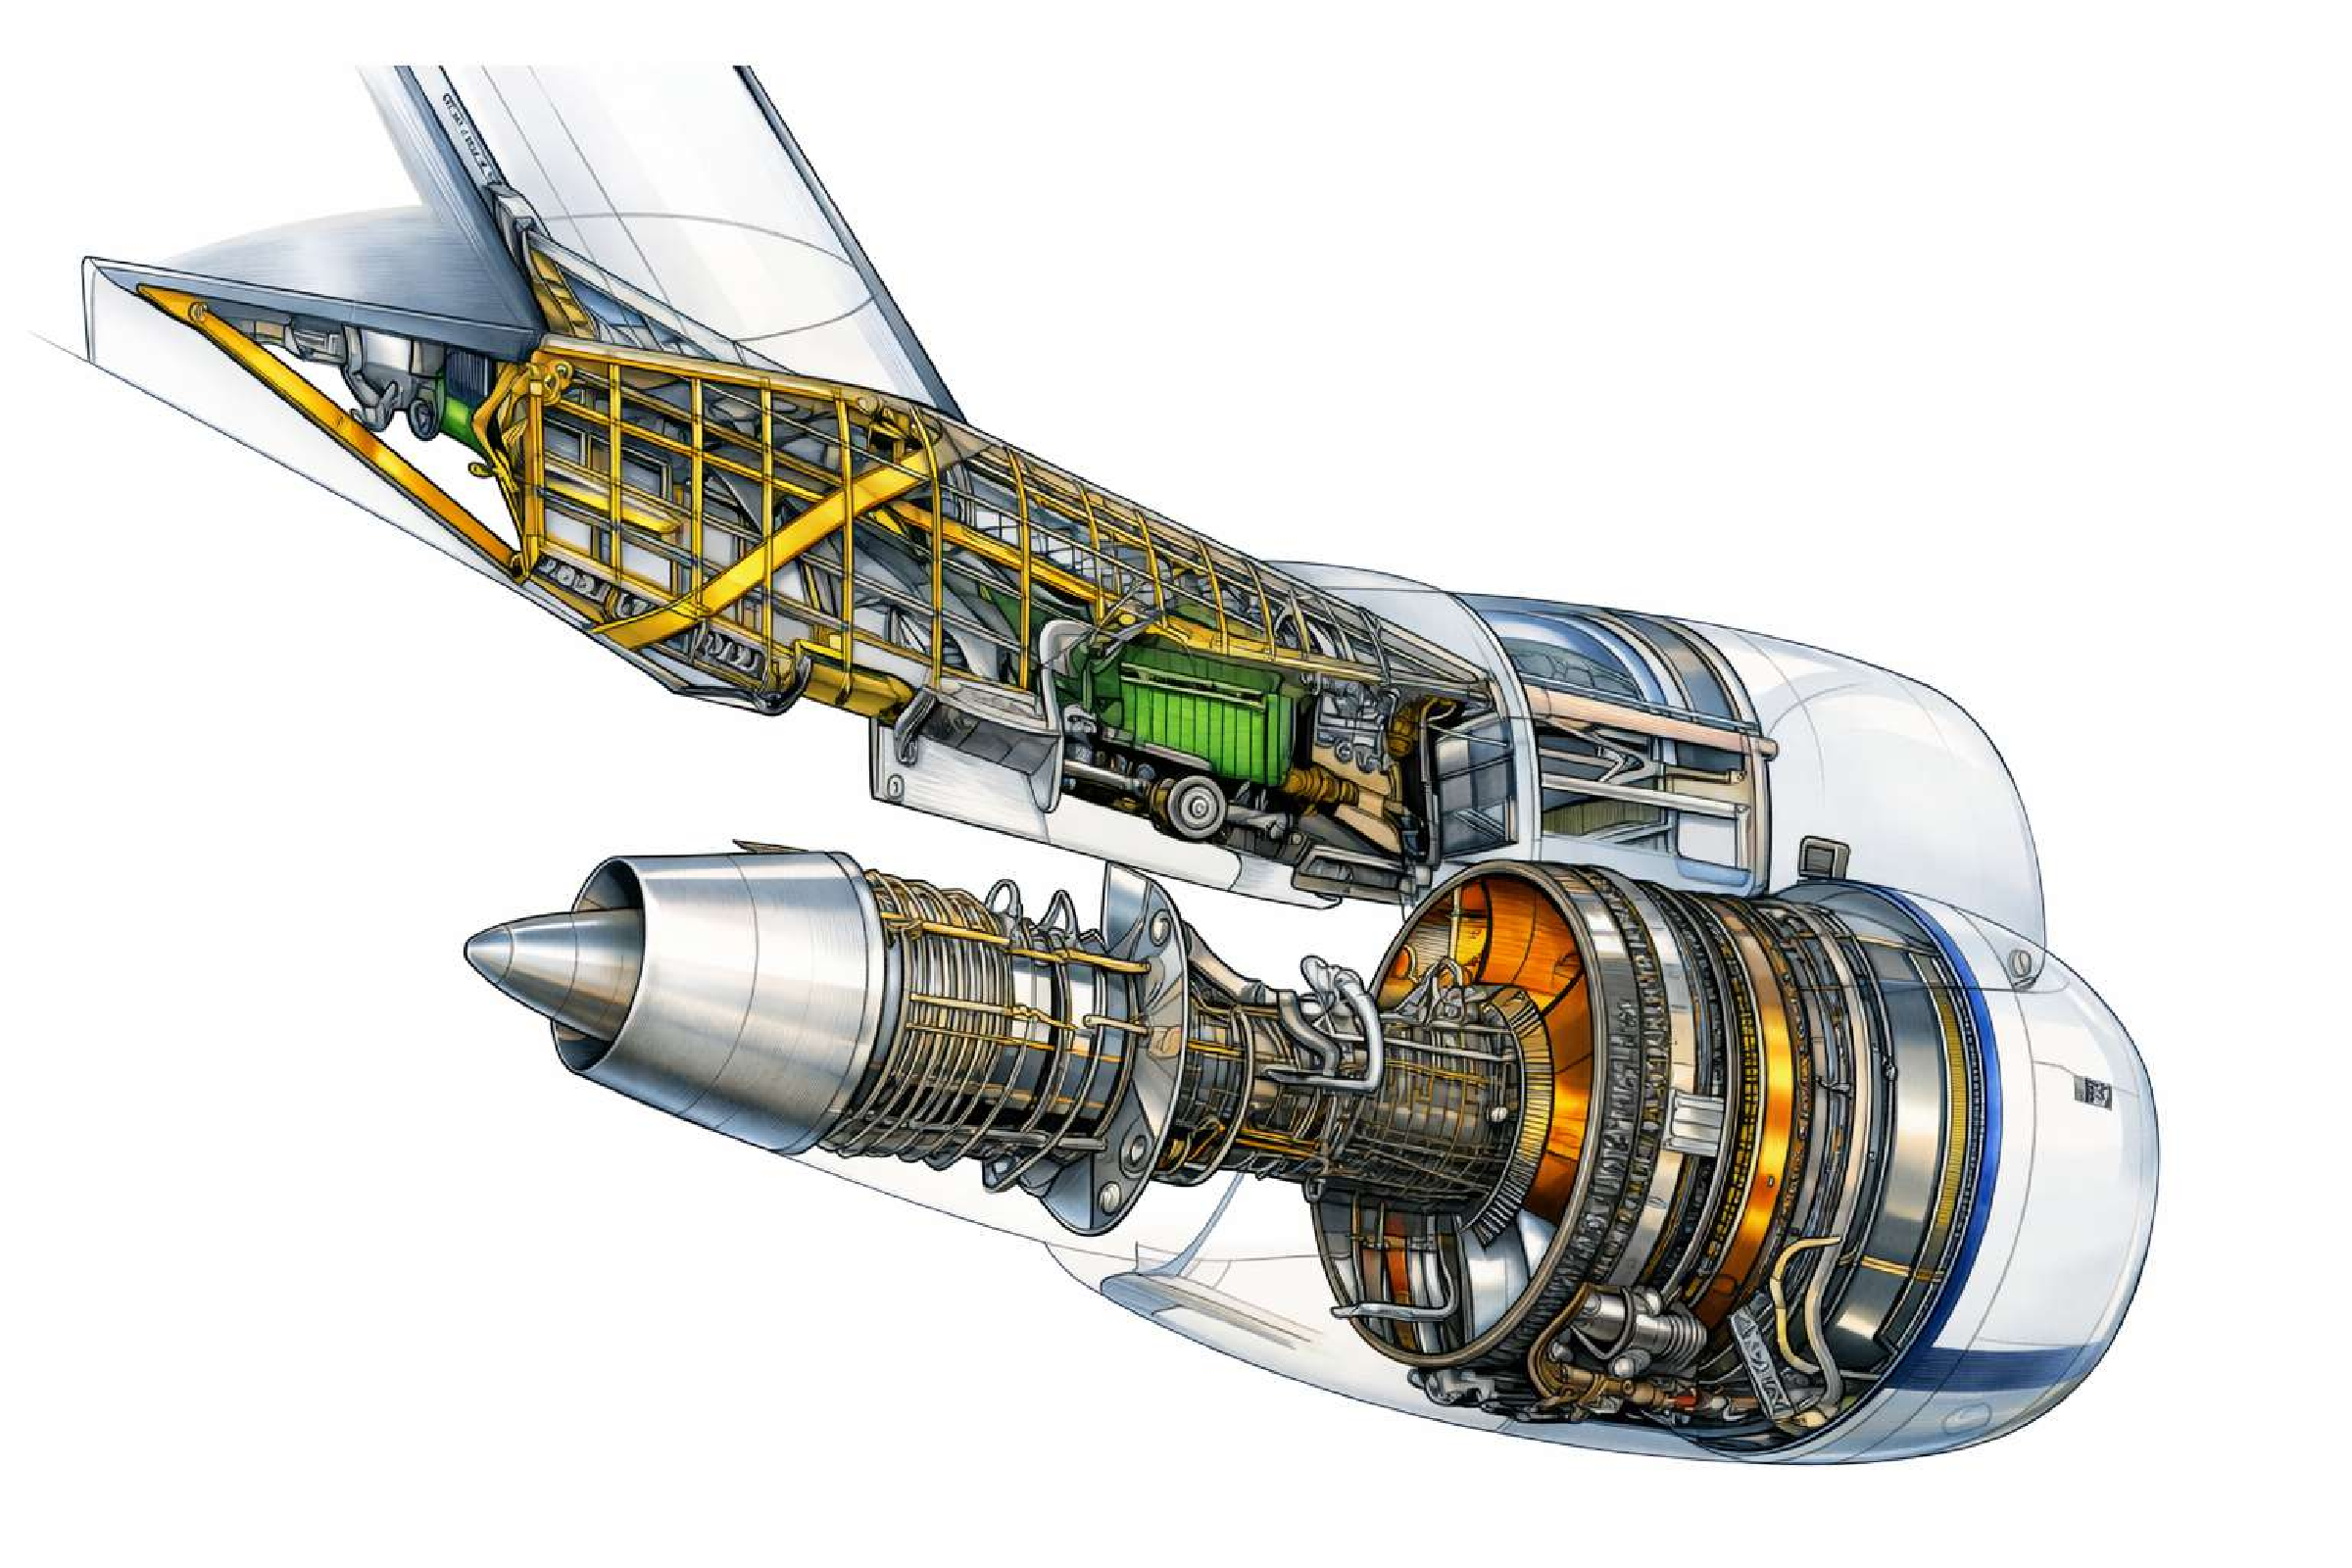
\includegraphics[width=\linewidth,
						height=0.27\paperheight, keepaspectratio]{aerospace}
					\end{minipage}
					\par\vspace{8pt}
					{\footnotesize\sffamily 航空航天承力结构}
				\end{tcolorbox}
			\end{column}
			
			\begin{column}{0.32\linewidth}
				\begin{tcolorbox}[
					enhanced, nobeforeafter,
					colback=white, colframe=structure.fg!25,
					boxrule=0.4pt, arc=2pt,
					left=3pt, right=3pt, top=4pt, bottom=4pt,
					width=\linewidth, height=0.40\paperheight,
					halign=center,
					]
					\centering
					\begin{minipage}[c][0.27\paperheight][c]{\linewidth}
						\centering
						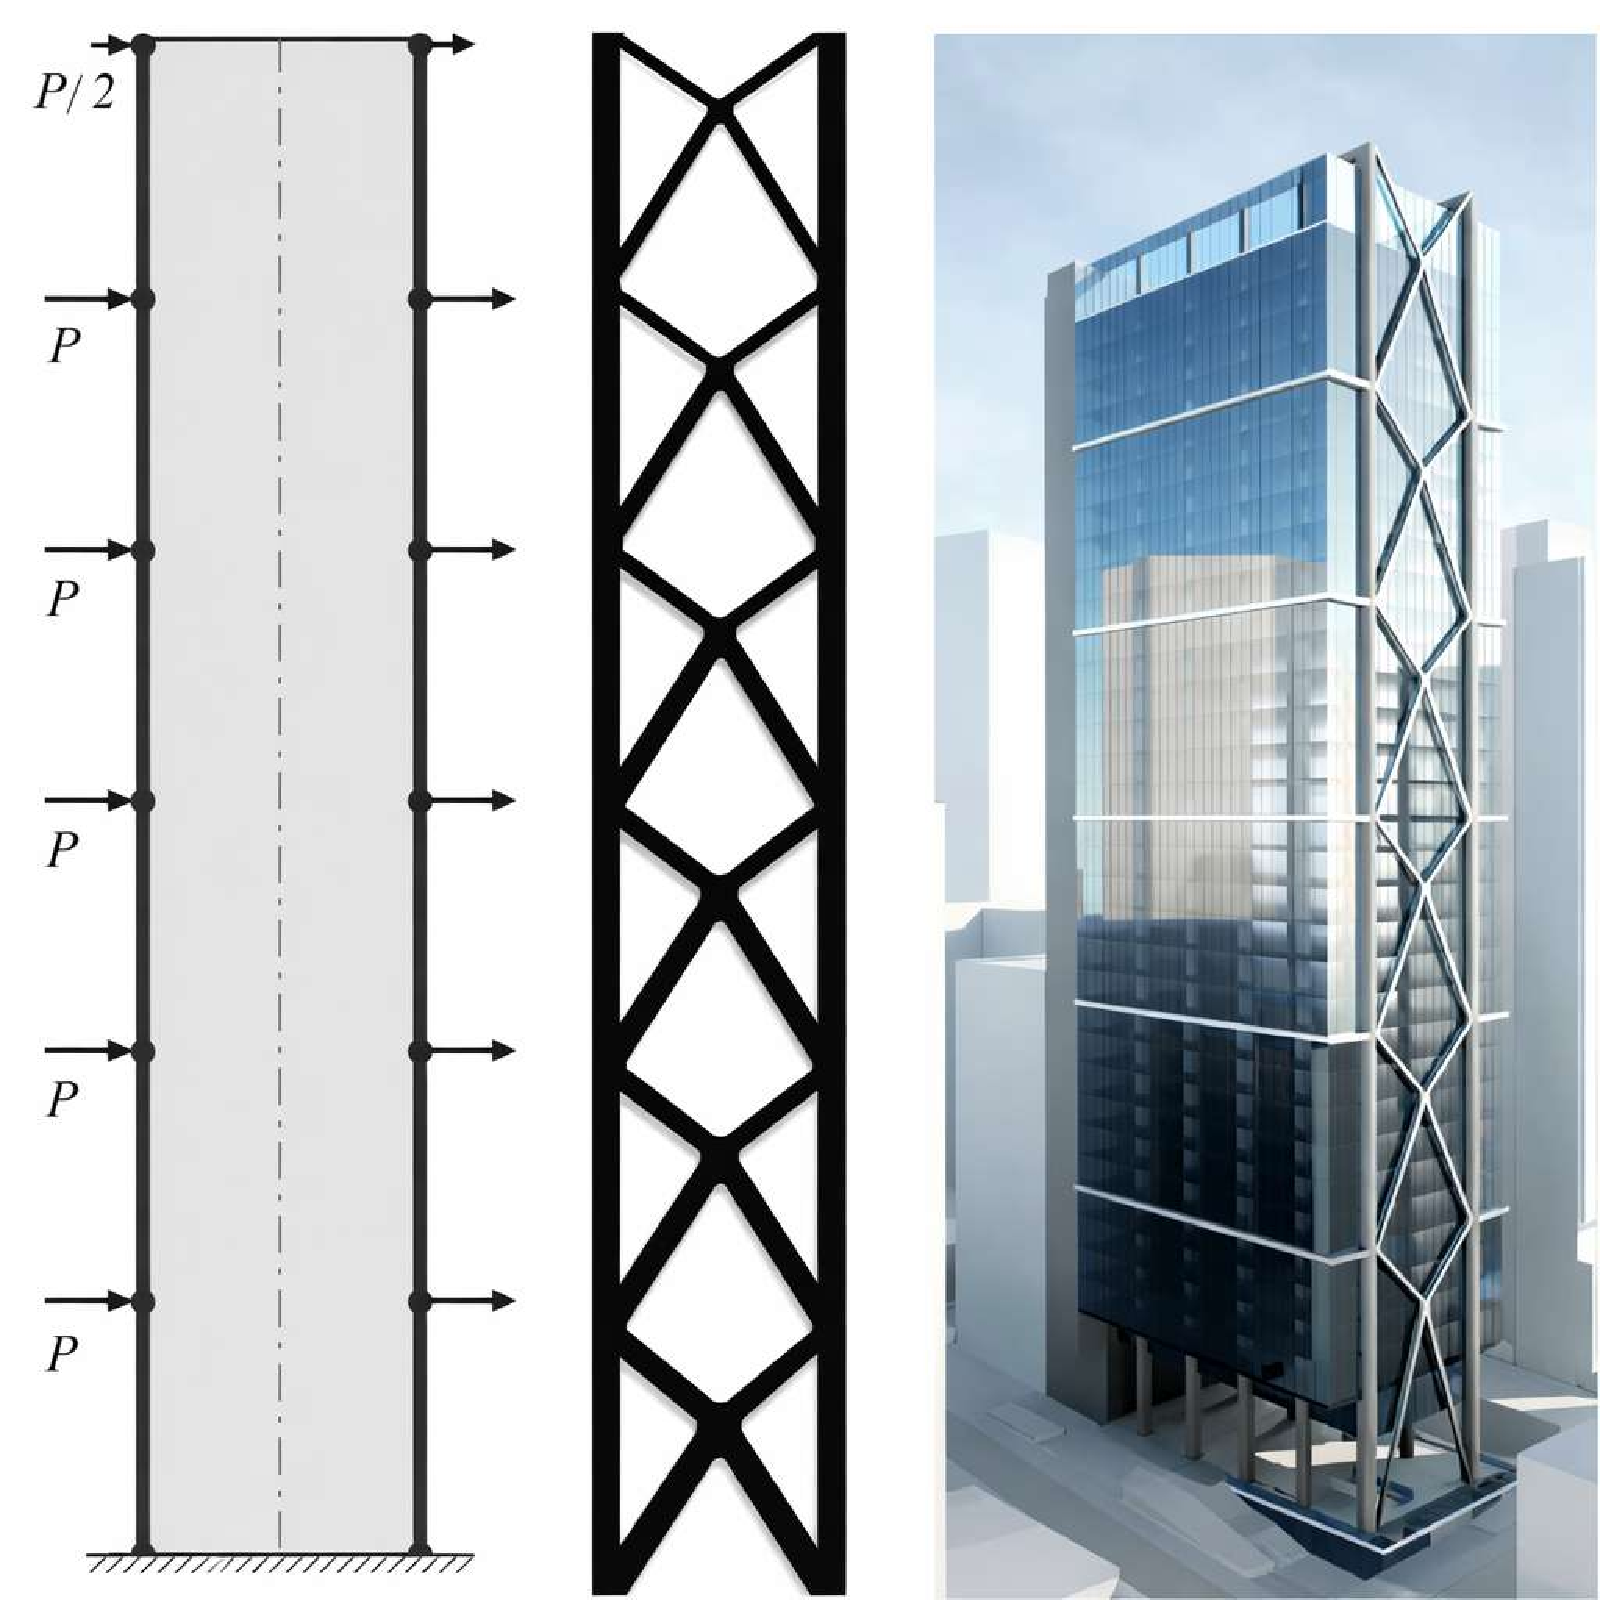
\includegraphics[width=\linewidth,
						height=0.27\paperheight, keepaspectratio]{building}
					\end{minipage}
					\par\vspace{8pt}
					{\footnotesize\sffamily 高层建筑抗侧力体系}
				\end{tcolorbox}
			\end{column}
			
			\begin{column}{0.32\linewidth}
				\begin{tcolorbox}[
					enhanced, nobeforeafter,
					colback=white, colframe=structure.fg!25,
					boxrule=0.4pt, arc=2pt,
					left=3pt, right=3pt, top=4pt, bottom=4pt,
					width=\linewidth, height=0.40\paperheight,
					halign=center,
					]
					\centering
					\begin{minipage}[c][0.27\paperheight][c]{\linewidth}
						\centering
						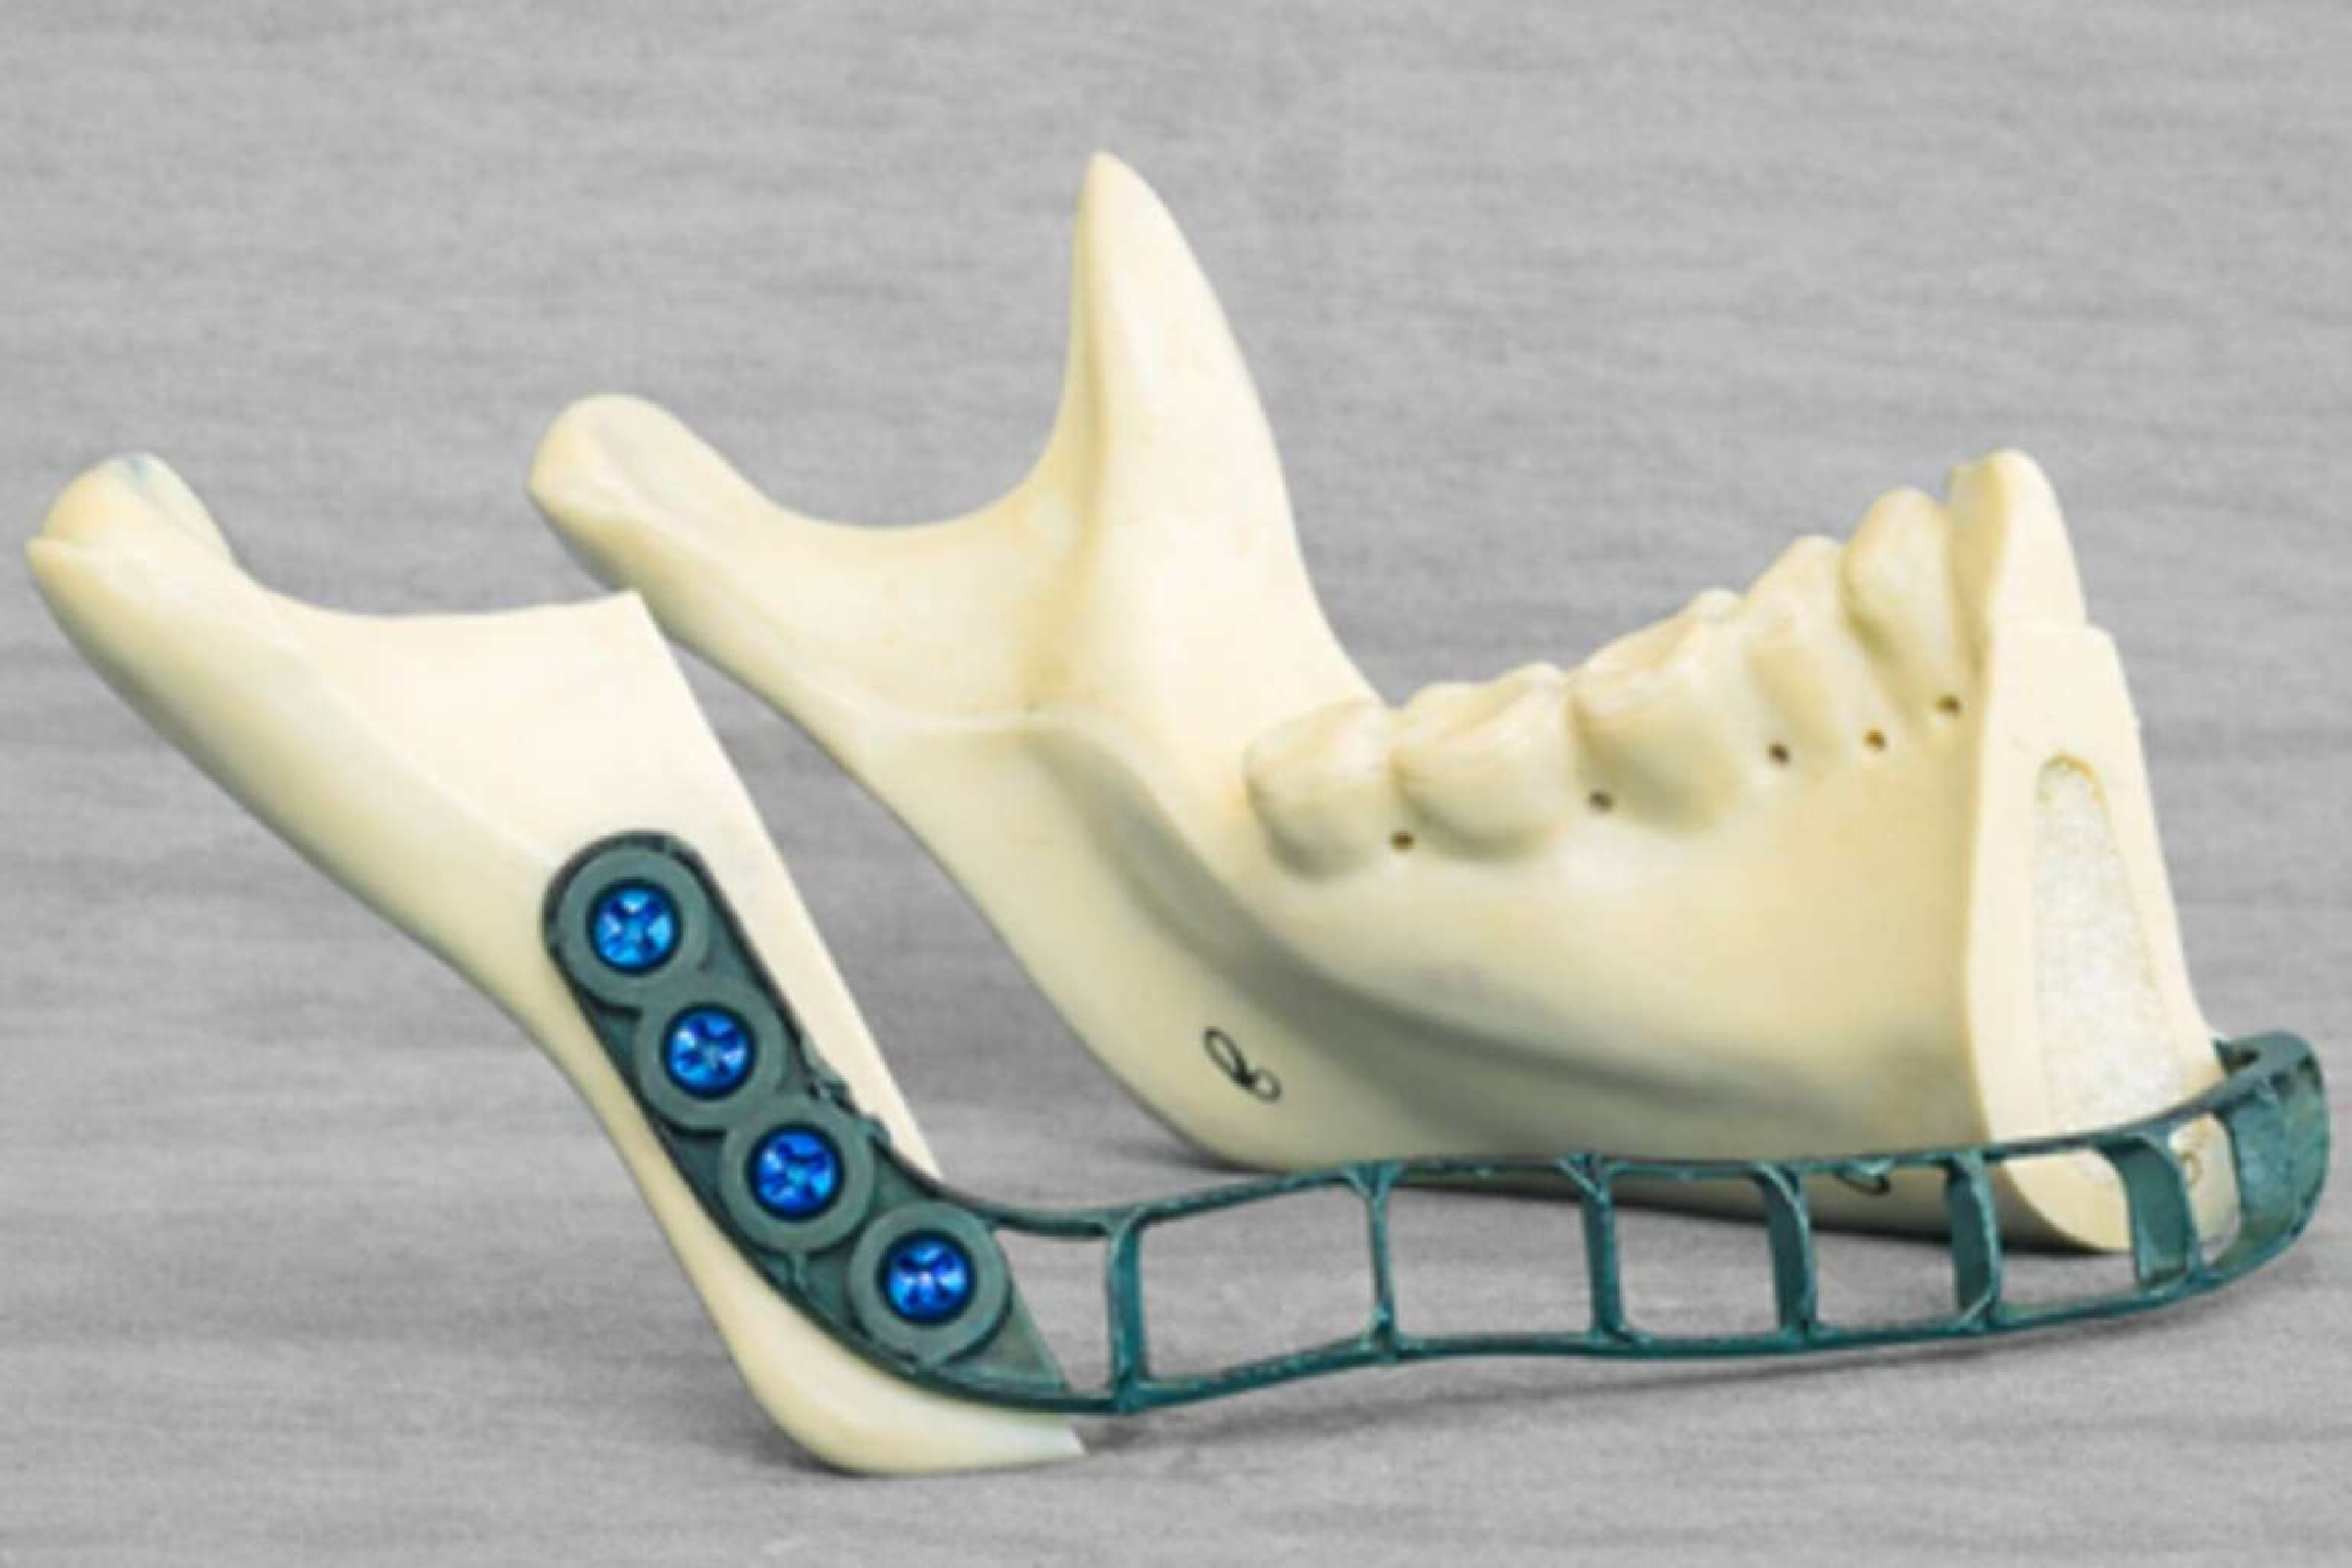
\includegraphics[width=\linewidth,
						height=0.27\paperheight, keepaspectratio]{biomedical}
					\end{minipage}
					\par\vspace{8pt}
					{\footnotesize\sffamily 个性化生物医疗植入体}
				\end{tcolorbox}
			\end{column}
			
		\end{columns}
		
		\vspace{1em}
		
		% ══════════════════════════════════════════════════════════
		%  底部文字区：三条递进式结论，1/2/3 编号，左对齐
		%  采用 \makebox + \parbox 组合保证编号列与正文列精准对齐
		% ══════════════════════════════════════════════════════════
		{\fontsize{8.5}{14}\selectfont\sffamily
			\noindent
			\makebox[1.5em][l]{\textbf{1}}%
			\parbox[t]{\dimexpr\linewidth - 1.5em\relax}{%
				复杂工程结构设计对轻量化、高性能与工程可行性提出了更高要求}
			
			\vspace{5pt}\noindent
			\makebox[1.5em][l]{\textbf{2}}%
			\parbox[t]{\dimexpr\linewidth - 1.5em\relax}{%
				结构优化设计逐步从尺寸优化、形状优化发展到拓扑优化}
			
			\vspace{5pt}\noindent
			\makebox[1.5em][l]{\textbf{3}}%
			\parbox[t]{\dimexpr\linewidth - 1.5em\relax}{%
				连续体结构拓扑优化以材料分布为设计对象，
				是性能驱动结构设计的重要数学工具}
		}
		
	\end{frame}
	
	% ============================================================
	%  01-2  变密度拓扑优化
	% ============================================================
	
	\begin{frame}
		\frametitle{变密度拓扑优化}
		
		% ── 顶部引导语 ───────────────────────────────────────────
		\begin{tcolorbox}[
			colback=panelbg, colframe=structure.fg!40,
			arc=3pt, boxrule=0.5pt,
			top=2pt, bottom=2pt, left=8pt, right=8pt]
			{\fontsize{8}{12}\selectfont\sffamily
				本文聚焦连续体结构变密度拓扑优化：以密度设计变量描述材料分布状态，%
				并通过正则化处理、有限元分析、灵敏度分析与优化更新构成计算闭环。}
		\end{tcolorbox}
		
		\vspace{-0.5em}
		
		% ── 中部主图：计算闭环流程 ─────────────────────────────
		\begin{tcolorbox}[
			colback=panelbg!40, colframe=structure.fg!50,
			colbacktitle=structure.fg, coltitle=white,
			fonttitle=\fontsize{7.5}{10}\selectfont\bfseries\sffamily,
			title={计算闭环流程},
			arc=3pt, boxrule=0.5pt,
			toptitle=2pt, bottomtitle=2pt,
			top=4pt, bottom=4pt, left=2pt, right=2pt]
			
			\centering
			\begin{tikzpicture}[
				box/.style={
					rectangle, rounded corners=2.5pt,
					draw=structure.fg!60, line width=0.4pt,
					fill=white,
					minimum width=1.85cm, minimum height=0.78cm,
					align=center, inner sep=1pt,
					font=\fontsize{6.5}{8}\selectfont\sffamily
				},
				boxstart/.style={
					box, fill=structure.fg!15,
					font=\fontsize{6.5}{8}\selectfont\sffamily\bfseries
				},
				boxend/.style={
					box, fill=structure.fg, text=white,
					font=\fontsize{6.5}{8}\selectfont\sffamily\bfseries
				},
				arrow/.style={
					-{Stealth[length=3.5pt]}, line width=0.55pt,
					draw=structure.fg!75
				},
				loop/.style={
					-{Stealth[length=3.5pt]}, line width=0.55pt,
					draw=structure.fg!75, dashed
				}
				]
				
				% ── 上排（左 → 右）─────────────────────────────────
				\node[boxstart] (n1)  at (0,    1.4) {设计域 $\Omega$};
				\node[box]      (n2)  at (2.25, 1.4) {密度设计变量 $\rho$};
				\node[box]      (n3)  at (4.50, 1.4) {正则化处理\\过滤 / 投影};
				\node[box]      (n4)  at (6.75, 1.4) {物理密度场 $\tilde{\rho}$};
				\node[box]      (n5)  at (9.00, 1.4) {材料属性插值\\$E(\tilde{\rho})$};
				
				% ── 下排（右 → 左）─────────────────────────────────
				\node[box]      (n6)  at (9.00, 0)   {有限元分析};
				\node[box]      (n7)  at (6.75, 0)   {目标 / 约束评估};
				\node[box]      (n8)  at (4.50, 0)   {灵敏度分析};
				\node[box]      (n9)  at (2.25, 0)   {优化更新};
				\node[boxend]   (n10) at (0,    0)   {拓扑构型};
				
				% ── 流程箭头
				\draw[arrow] (n1) -- (n2);
				\draw[arrow] (n2) -- (n3);
				\draw[arrow] (n3) -- (n4);
				\draw[arrow] (n4) -- (n5);
				\draw[arrow] (n5) -- (n6);
				\draw[arrow] (n6) -- (n7);
				\draw[arrow] (n7) -- (n8);
				\draw[arrow] (n8) -- (n9);
				\draw[arrow] (n9) -- (n10);
				
				% ── 闭环反馈
				\draw[loop] (n9.north) -- (n2.south)
				node[midway, right=2pt,
				font=\fontsize{5.5}{7}\selectfont\sffamily,
				text=structure.fg!85] {返回更新 $\rho$};
				
			\end{tikzpicture}
			
		\end{tcolorbox}
		
		% ── 下方三点说明 ────────────────────────────────────────
		{\fontsize{8}{12}\selectfont\sffamily
			\noindent
			\makebox[2em][l]{\textbf{01}}%
			\parbox[t]{\dimexpr\linewidth - 2em\relax}{%
				\textbf{设计对象：}给定设计域内的材料空间分布}
			
			\vspace{3pt}\noindent
			\makebox[2em][l]{\textbf{02}}%
			\parbox[t]{\dimexpr\linewidth - 2em\relax}{%
				\textbf{方法特征：}用连续取值的密度设计变量表征材料分布状态}
			
			\vspace{3pt}\noindent
			\makebox[2em][l]{\textbf{03}}%
			\parbox[t]{\dimexpr\linewidth - 2em\relax}{%
				\textbf{计算核心：}正则化处理、有限元分析、灵敏度分析与优化更新形成闭环}
		}
		
	\end{frame}
	
	% ============================================================
	%  01-3  分析精度与拓扑分辨率的双重瓶颈
	% ============================================================
	
	\begin{frame}
		\frametitle{分析精度与拓扑分辨率的双重瓶颈}
		
		% ── 顶部引导语 ───────────────────────────────────────────
		\begin{tcolorbox}[
			colback=panelbg, colframe=structure.fg!40,
			arc=3pt, boxrule=0.5pt,
			top=2pt, bottom=2pt, left=8pt, right=8pt]
			{\fontsize{8}{12}\selectfont\sffamily
				传统变密度拓扑优化在复杂结构设计中，面临低阶有限元分析精度不足%
				与单分辨率框架表达能力受限的双重瓶颈。}
		\end{tcolorbox}
		
		\vspace{-1.4em}
		
		% ── 中部主体：左右两栏 ─────────────────────────────────
		\begin{columns}[T,onlytextwidth]
			
			% 左栏：分析精度瓶颈
			\begin{column}{0.485\textwidth}
				\begin{tcolorbox}[
					colback=panelbg!35, colframe=structure.fg!50,
					colbacktitle=structure.fg, coltitle=white,
					fonttitle=\fontsize{7.5}{10}\selectfont\bfseries\sffamily,
					title={分析精度瓶颈},
					arc=3pt, boxrule=0.5pt,
					toptitle=2pt, bottomtitle=2pt,
					top=5pt, bottom=5pt, left=6pt, right=6pt,
					height=4.5cm]
					
					{\fontsize{7.5}{11}\selectfont\sffamily
						\textcolor{structure.fg}{\textbf{低阶位移有限元的局限}}
						
						\vspace{0.5em}
						
						\begin{itemize}
							\setlength{\itemsep}{4pt}
							\item 复杂变形模式刻画能力有限
							\item 局部应力场由位移梯度后处理得到，精度受限
							\item 近不可压缩材料易出现体积闭锁
						\end{itemize}
						
						\vfill
						
						\textcolor{structure.fg}{\(\Rightarrow\)}
						难以可靠支撑高精度力学场刻画与局部力学约束评估。
					}
					
				\end{tcolorbox}
			\end{column}
			
			% 右栏：拓扑分辨率瓶颈
			\begin{column}{0.485\textwidth}
				\begin{tcolorbox}[
					colback=panelbg!35, colframe=structure.fg!50,
					colbacktitle=structure.fg, coltitle=white,
					fonttitle=\fontsize{7.5}{10}\selectfont\bfseries\sffamily,
					title={拓扑分辨率瓶颈},
					arc=3pt, boxrule=0.5pt,
					toptitle=2pt, bottomtitle=2pt,
					top=5pt, bottom=5pt, left=6pt, right=6pt,
					height=4.5cm]
					
					{\fontsize{7.5}{11}\selectfont\sffamily
						\textcolor{structure.fg}{\textbf{单分辨率框架的局限}}
						
						\vspace{0.5em}
						
						\begin{itemize}
							\setlength{\itemsep}{4pt}
							\item 分析网格与设计网格严格绑定
							\item 提高设计分辨率会显著增加计算规模
							\item 提高有限元阶次不等价于提高拓扑表达分辨率
						\end{itemize}
						
						\vfill
						
						\textcolor{structure.fg}{\(\Rightarrow\)}
						难以同时兼顾高精度分析与高分辨率拓扑表达。
					}
					
				\end{tcolorbox}
			\end{column}
			
		\end{columns}
		
		% ── 底部结论条 ───────────────────────────────────────────
		\begin{tcolorbox}[
			colback=structure.fg, colframe=structure.fg,
			arc=3pt, boxrule=0pt,
			top=3.5pt, bottom=3.5pt, left=8pt, right=8pt]
			\centering
			{\fontsize{8}{11}\selectfont\sffamily\color{white}
				\textbf{核心矛盾：}传统框架难以在可控计算规模下，
				同时获得准确力学场刻画与细致拓扑构型}
		\end{tcolorbox}
		
	\end{frame}
	
	% ============================================================
	%  01-4  拓扑优化的软件生态与实现瓶颈
	% ============================================================
	
	\begin{frame}
		\frametitle{拓扑优化的软件生态与实现瓶颈}
		
		% ── 顶部引导语 ───────────────────────────────────────────
		\begin{tcolorbox}[
			colback=panelbg, colframe=structure.fg!40,
			arc=3pt, boxrule=0.5pt,
			top=2pt, bottom=2pt, left=8pt, right=8pt]
			{\fontsize{8}{12}\selectfont\sffamily
				先进拓扑优化方法走向复杂工程应用，不仅依赖数学模型与数值算法，%
				也需要统一、可扩展且高性能的软件平台支撑。}
		\end{tcolorbox}
		
		\vspace{-1.2em}
		
		% ── 中部主体：三块并列 ─────────────────────────────────
		\begin{columns}[T,onlytextwidth]
			
			\begin{column}{0.315\textwidth}
				\begin{tcolorbox}[
					colback=panelbg!35, colframe=structure.fg!50,
					colbacktitle=structure.fg, coltitle=white,
					fonttitle=\fontsize{7.2}{9.5}\selectfont\bfseries\sffamily,
					title={01 \quad 算法实现耦合严重},
					arc=3pt, boxrule=0.5pt,
					toptitle=2pt, bottomtitle=2pt,
					top=5pt, bottom=5pt, left=5pt, right=5pt,
					height=3.6cm]
					{\fontsize{7.2}{10.5}\selectfont\sffamily
						\setbeamertemplate{itemize item}{\raisebox{1pt}{\tiny$\bullet$}}
						\setlength{\leftmargini}{0.8em}
						
						\begin{itemize}
							\setlength{\itemsep}{4pt}
							\item 有限元分析、灵敏度分析与优化更新紧密耦合
							\item 新模型、新正则化策略扩展成本高
							\item 算法复现与跨问题迁移困难
						\end{itemize}
					}
				\end{tcolorbox}
			\end{column}
			
			\begin{column}{0.315\textwidth}
				\begin{tcolorbox}[
					colback=panelbg!35, colframe=structure.fg!50,
					colbacktitle=structure.fg, coltitle=white,
					fonttitle=\fontsize{7.2}{9.5}\selectfont\bfseries\sffamily,
					title={02 \quad 先进离散方法支撑不足},
					arc=3pt, boxrule=0.5pt,
					toptitle=2pt, bottomtitle=2pt,
					top=5pt, bottom=5pt, left=5pt, right=5pt,
					height=3.6cm]
					{\fontsize{7.2}{10.5}\selectfont\sffamily
						\setbeamertemplate{itemize item}{\raisebox{1pt}{\tiny$\bullet$}}
						\setlength{\leftmargini}{0.8em}
						
						\begin{itemize}
							\setlength{\itemsep}{4pt}
							\item 高阶有限元、混合元、多分辨率框架难以统一组织
							\item 理论方法与工程实现之间存在断层
							\item 缺少面向拓扑优化闭环的模块化接口
						\end{itemize}
					}
				\end{tcolorbox}
			\end{column}
			
			\begin{column}{0.315\textwidth}
				\begin{tcolorbox}[
					colback=panelbg!35, colframe=structure.fg!50,
					colbacktitle=structure.fg, coltitle=white,
					fonttitle=\fontsize{7.2}{9.5}\selectfont\bfseries\sffamily,
					title={03 \quad 高性能计算能力不足},
					arc=3pt, boxrule=0.5pt,
					toptitle=2pt, bottomtitle=2pt,
					top=5pt, bottom=5pt, left=5pt, right=5pt,
					height=3.6cm]
					{\fontsize{7.2}{10.5}\selectfont\sffamily
						\setbeamertemplate{itemize item}{\raisebox{1pt}{\tiny$\bullet$}}
						\setlength{\leftmargini}{0.8em}
						
						\begin{itemize}
							\setlength{\itemsep}{4pt}
							\item 大规模问题中矩阵组装与线性求解开销显著
							\item 缺少自动微分灵敏度分析支撑
							\item 多后端与 CPU/GPU 异构执行能力不足
						\end{itemize}
					}
				\end{tcolorbox}
			\end{column}
			
		\end{columns}
		
		\vspace{0.2em}
		
		% ── 底部结论条 ───────────────────────────────────────────
		\begin{tcolorbox}[
			colback=structure.fg, colframe=structure.fg,
			arc=3pt, boxrule=0pt,
			top=3.5pt, bottom=3.5pt, left=8pt, right=8pt]
			\centering
			{\fontsize{8}{11}\selectfont\sffamily\color{white}
				统一、可扩展的高性能软件平台，是推动先进拓扑优化方法走向可复现工程计算的关键支撑。}
		\end{tcolorbox}
		
	\end{frame}
	
	% ============================================================
	%  01-5  关键问题与本文思路
	% ============================================================
	\begin{frame}
		\frametitle{关键问题与本文思路}
		
		% ── 顶部一句话 ───────────────────────────────────────────
		\begin{tcolorbox}[
			colback=panelbg, colframe=structure.fg!40,
			arc=3pt, boxrule=0.5pt,
			top=2pt, bottom=2pt, left=8pt, right=8pt]
			{\fontsize{8}{12}\selectfont\sffamily
				连续体变密度拓扑优化在复杂工程应用中，需要同时兼顾高精度分析、%
				高分辨率表达、复杂局部约束处理与高效软件实现。}
		\end{tcolorbox}
		
		\vspace{-0.6em}
		
		% ── 中部：关键问题 ⇒ 本文思路 对照表（手工 makebox 行式）─
		\begin{tcolorbox}[
			colback=white, colframe=structure.fg!50,
			arc=3pt, boxrule=0.5pt,
			top=4pt, bottom=4pt, left=12pt, right=12pt,
			boxsep=2pt]%
			\setlength{\parskip}{0pt}\setlength{\parindent}{0pt}%
			\fontsize{9}{12}\selectfont\sffamily%
			%% —— 表头 ——
			\makebox[0.40\linewidth][l]{\bfseries\color{structure.fg}关键问题}%
			\makebox[0.06\linewidth][c]{}%
			\makebox[0.50\linewidth][l]{\bfseries\color{structure.fg}本文思路}\par
			\vspace{8pt}%
			%% —— 行 01 ——
			\makebox[0.40\linewidth][l]{\circnum{01}~分析精度受限}%
			\makebox[0.06\linewidth][c]{\color{structure.fg!70}$\Rightarrow$}%
			\makebox[0.50\linewidth][l]{引入任意次拉格朗日有限元}\par
			\vspace{5pt}%
			%% —— 行 02 ——
			\makebox[0.40\linewidth][l]{\circnum{02}~分辨率与规模矛盾}%
			\makebox[0.06\linewidth][c]{\color{structure.fg!70}$\Rightarrow$}%
			\makebox[0.50\linewidth][l]{构建高阶多分辨率拓扑优化框架}\par
			\vspace{5pt}%
			%% —— 行 03 ——
			\makebox[0.40\linewidth][l]{\circnum{03}~局部约束处理困难}%
			\makebox[0.06\linewidth][c]{\color{structure.fg!70}$\Rightarrow$}%
			\makebox[0.50\linewidth][l]{发展胡张混合有限元拓扑优化方法}\par
			\vspace{5pt}%
			%% —— 行 04 ——
			\makebox[0.40\linewidth][l]{\circnum{04}~统一实现支撑不足}%
			\makebox[0.06\linewidth][c]{\color{structure.fg!70}$\Rightarrow$}%
			\makebox[0.50\linewidth][l]{设计高性能软件平台 SOPTX}%
		\end{tcolorbox}
		
		\vspace{-0.6em}
		
		% ── 底部结论 ─────────────────────────────────────────────
		\begin{tcolorbox}[
			colback=structure.fg, colframe=structure.fg,
			arc=3pt, boxrule=0pt,
			top=3.5pt, bottom=3.5pt, left=8pt, right=8pt]
			\centering
			{\fontsize{8}{12}\selectfont\sffamily\color{white}
				本文形成“高阶有限元分析—多分辨率计算—混合建模—软件实现”的系统研究路线。}
		\end{tcolorbox}
		
	\end{frame}

	
	% ============================================================
	\section{变密度拓扑优化的数学框架}
	% ============================================================
	
	% ============================================================
	%  02-1  材料密度与插值模型
	% ============================================================
	
	\begin{frame}
		\frametitle{材料密度与插值模型}
		
		\vspace{-0.8em}
		
		% ══════════════════════════════════════════════════════════
		%  主体双栏：左侧变量连续化 / 右侧 SIMP 惩罚机制
		% ══════════════════════════════════════════════════════════
		\begin{columns}[T, totalwidth=\linewidth]
			
			% ─── 左栏：从 0-1 离散分布到变量连续化 ───────────────────
			\begin{column}{0.485\linewidth}
				\begin{tcolorbox}[
					colback=white, colframe=structure.fg!50,
					colbacktitle=structure.fg, coltitle=white,
					fonttitle=\fontsize{8}{10}\selectfont\bfseries\sffamily,
					title={变量连续化：从离散到连续},
					arc=3pt, boxrule=0.5pt,
					toptitle=3pt, bottomtitle=3pt,
					top=4pt, bottom=4pt, left=6pt, right=6pt,
					height=0.63\paperheight, valign=top]
					{\fontsize{7.5}{9.5}\selectfont\sffamily
						\setbeamertemplate{itemize item}{\raisebox{1pt}{\tiny$\bullet$}}
						\setlength{\leftmargini}{0.8em}
						
						\textbf{\circnum{01}\enspace 拓扑优化的本质}\par
						\vspace{2pt}
						\begin{itemize}
							\item 寻找最优特征函数 $\chi(\boldsymbol{x}) \in \{0, 1\}$（$1$: \textbf{实体材料}, $0$: \textbf{孔洞区域}）；
							\item 属于大规模非凸整型规划，难以利用基于梯度的求解算法。
						\end{itemize}
						
						\textbf{\circnum{02}\enspace 引入连续密度场}\par
						\vspace{2pt}
						\begin{itemize}
							\item 将 $\chi$ 松弛为连续标量场:
							\vspace{-4pt}
							\begin{equation*}
								\rho(\boldsymbol{x}) \in [0, 1], \quad \forall \boldsymbol{x} \in \Omega
							\end{equation*}
							
							\vspace{-8pt}
							\item $\rho = 1$ 表示\textbf{实体材料}，$\rho = 0$ 表示\textbf{孔洞区域}，$0 < \rho < 1$ 表示\textbf{中间密度}。
						\end{itemize}
					}
				\end{tcolorbox}
			\end{column}
			
			% ─── 右栏：SIMP 插值与惩罚机制 ───────────────────────────
			\begin{column}{0.485\linewidth}
				\begin{tcolorbox}[
					colback=white, colframe=structure.fg!50,
					colbacktitle=structure.fg, coltitle=white,
					fonttitle=\fontsize{8}{10}\selectfont\bfseries\sffamily,
					title={SIMP 插值模型与惩罚机制},
					arc=3pt, boxrule=0.5pt,
					toptitle=3pt, bottomtitle=3pt,
					top=6pt, bottom=6pt, left=6pt, right=6pt,
					height=0.63\paperheight, valign=top]
					{\fontsize{7.5}{10.5}\selectfont\sffamily
						\setbeamertemplate{itemize item}{\raisebox{1pt}{\tiny$\bullet$}}
						\setlength{\leftmargini}{0.8em}
						
						\textbf{\circnum{01}\enspace 固体各向同性材料插值}\par
						\vspace{2pt}
						\begin{itemize}
							\item 通过该模型建立弹性模量与密度的非线性映射：
							\vspace{-8pt}
							\begin{equation*}
								E(\rho) = E_{\min} + \rho^{p} (E_0 - E_{\min})
							\end{equation*}
							
							\vspace{-8pt}
							{\color{gray}\fontsize{6.5}{8}\selectfont $E_{\min}$ 为避免刚度矩阵奇异的极小值}\par
						\end{itemize}
						
						\textbf{\circnum{02}\enspace 惩罚效应与二值化趋势}\par
						\vspace{2pt}
						\begin{itemize}
							\item 引入惩罚因子 $p$（常取 $p \ge 3$），降低中间密度（灰度区域）的相对刚度贡献
							\item 促使设计变量在优化迭代中向 $0$ 或 $1$ 两端收敛，获得几何边界清晰的拓扑构型
						\end{itemize}
					}
				\end{tcolorbox}
			\end{column}
			
		\end{columns}
		
		\vspace{0.4em}
		
		% ── 底部结论条 ───────────────────────────────────────────
		\begin{tcolorbox}[
			colback=structure.fg, colframe=structure.fg,
			arc=3pt, boxrule=0pt,
			top=3.5pt, bottom=3.5pt, left=8pt, right=8pt]
			\centering
			{\fontsize{8}{11}\selectfont\sffamily\color{white}
				构建\textbf{密度场 $\rho(\boldsymbol{x})$} 与 \textbf{SIMP 惩罚插值}，是变密度拓扑优化的核心基石}
		\end{tcolorbox}
		
	\end{frame}
	
	% ============================================================
	%  02-2  变密度拓扑优化的数学模型
	% ============================================================
	
	\begin{frame}
		\frametitle{变密度拓扑优化的数学模型}
		
		\vspace{-0.5em}
		
		\begin{tcolorbox}[
			colback=white, colframe=structure.fg!50,
			colbacktitle=structure.fg, coltitle=white,
			fonttitle=\fontsize{9}{11}\selectfont\bfseries\sffamily,
			title={连续域下的 PDE 约束优化问题},
			arc=3pt, boxrule=0.5pt,
			toptitle=4pt, bottomtitle=4pt,
			top=10pt, bottom=10pt, left=10pt, right=10pt]
			
			{\fontsize{8.5}{13}\selectfont\sffamily
				在连续空间中寻找最优材料分布（密度场） $\rho(\boldsymbol{x})\in{L}^{\infty}(\Omega)$，其数学模型通常表述为：
				
				\begin{equation*}
					\left\{
					\begin{aligned}
						\min_{\rho} \quad & \mathcal{J}(\boldsymbol{u}, \rho) \quad (\text{目标泛函})\\
						\text{s.t.} \quad & a_{\rho}(\boldsymbol{u}, \boldsymbol{v}) = \ell(\boldsymbol{v}), \quad \forall \boldsymbol{v} \in \mathcal{V}_0 \quad (\text{状态方程}) \\
						& \mathcal{G}_i(\rho, \boldsymbol{u}) \le 0, \quad i = 1, \dots, m \quad (\text{不等式约束}) \\
						& 0 \le \rho(\boldsymbol{x}) \le 1, \quad \text{a.e. in } \Omega
					\end{aligned}
					\right.
				\end{equation*}
				
				\vspace{8pt}
				
				\begin{itemize}
					\item 目标泛函：衡量结构性能的泛函，如柔顺度、位移、应力或自振频率等；
					\item 状态方程：描述物理场的 PDE 变分形式，$a_{\rho}(\cdot, \cdot)$ 为依赖于密度的双线性型；
					\item 不等式约束：代表资源限制（如体积约束）或性能指标要求（如应力约束）。
				\end{itemize}
			}
		\end{tcolorbox}
		
	\end{frame}
	
	% ============================================================
	%  02-3  典型拓扑优化问题的数学模型
	% ============================================================
	
	\begin{frame}
		\frametitle{典型拓扑优化问题的数学模型}
		
		\vspace{-0.5em}
		
		\begin{tcolorbox}[
			colback=white, colframe=structure.fg!50,
			colbacktitle=structure.fg, coltitle=white,
			fonttitle=\fontsize{9}{11}\selectfont\bfseries\sffamily,
			title={\only<1>{柔顺度最小化问题}\only<2>{柔顺机构设计问题}\only<3>{应力约束问题}},
			arc=3pt, boxrule=0.5pt,
			toptitle=4pt, bottomtitle=4pt,
			top=10pt, bottom=10pt, left=10pt, right=10pt]
			
			{\fontsize{8.5}{13}\selectfont\sffamily
				
				% --- 1. 柔顺度最小化问题 ---
				\only<1>{
					目标是最大化结构在给定载荷下的整体刚度（即最小化柔顺度）：
					\begin{equation*}
						\left\{
						\begin{aligned}
							\min_{\rho} \quad & c(\boldsymbol{u}, \rho) = \int_{\Omega} (\mathbb{C}(\rho) : \boldsymbol{\varepsilon}(\boldsymbol{u})) : \boldsymbol{\varepsilon}(\boldsymbol{u}) \,\mathrm{d}\boldsymbol{x} \\
							\text{s.t.} \quad & a_{\rho}(\boldsymbol{u}, \boldsymbol{v}) = \ell(\boldsymbol{v}), \quad \forall \boldsymbol{v} \in \mathcal{V}_0 \\
							& \frac{V(\rho)}{V_0} \le V_f, \quad \text{其中 } V(\rho) = \int_{\Omega} \rho(\boldsymbol{x}) \,\mathrm{d}\boldsymbol{x} \\
							& 0 \le \rho(\boldsymbol{x}) \le 1, \quad \text{a.e. in } \Omega
						\end{aligned}
						\right.
					\end{equation*}
					\begin{itemize}
						\item \textbf{物理内涵}：在平衡状态下，最小化外力做功 $\ell(\boldsymbol{u})$ 等价于最小化结构总应变能；
						\item \textbf{数学特性}：自伴随问题，其灵敏度分析仅依赖于原状态变量 $\boldsymbol{u}$。
					\end{itemize}
				}
				
				% --- 2. 柔性机构设计问题 ---
				\only<2>{
					通过拓扑构型实现运动或力的预设传递，最大化指定端口的输出位移：
					\begin{equation*}
						\left\{
						\begin{aligned}
							\max_{\rho} \quad & \ell_{\text{out}}(\boldsymbol{u}) = \int_{\Gamma_{\text{out}}} \boldsymbol{d}_{\text{out}} \cdot \boldsymbol{u} \,\mathrm{d}s \\
							\text{s.t.} \quad & a_{\rho}(\boldsymbol{u}, \boldsymbol{v}) + s(\boldsymbol{u}, \boldsymbol{v}) = \ell_{\text{in}}(\boldsymbol{v}), \quad \forall \boldsymbol{v} \in \mathcal{V}_0 \\
							& \frac{V(\rho)}{V_0} \le V_f, \quad \text{其中 } V(\rho) = \int_{\Omega} \rho(\boldsymbol{x}) \,\mathrm{d}\boldsymbol{x} \\
							& 0 \le \rho(\boldsymbol{x}) \le 1, \quad \text{a.e. in } \Omega
						\end{aligned}
						\right.
					\end{equation*}
					其中 $\ell_{\text{in}}$ 为输入载荷泛函，$s(\boldsymbol{u}, \boldsymbol{v})$ 为附加弹簧刚度双线性型。
					\begin{itemize}
						\item \textbf{建模特征}：在输入/输出端引入弹簧刚度 $s(\boldsymbol{u}, \boldsymbol{v})$，避免“机制解”并表征致动器与工件的等效刚度；
						\item \textbf{数学特性}：非自伴随，灵敏度分析需求解以伴随载荷 $-\ell_{\text{out}}$ 为右端的伴随方程。
					\end{itemize}
				}
				
				% --- 3. 应力约束问题 ---
				\only<3>{
					在保证局部强度的前提下追求结构轻量化，是工程设计的核心需求：
					\begin{equation*}
						\left\{
						\begin{aligned}
							\min_{\rho} \quad & \mathcal{J}(\boldsymbol{u}, \rho) \\
							\text{s.t.} \quad & a_{\rho}(\boldsymbol{u}, \boldsymbol{v}) = \ell(\boldsymbol{v}), \quad \forall \boldsymbol{v} \in \mathcal{V}_0 \\
							& \sigma^{\text{vM}}(\boldsymbol{u})(\boldsymbol{x}) \le \bar{\sigma}, \quad \forall \boldsymbol{x} \in \Omega \setminus \Omega_{\text{void}} \\
							& 0 \le \rho(\boldsymbol{x}) \le 1, \quad \text{a.e. in } \Omega
						\end{aligned}
						\right.
					\end{equation*}
					其中 $\sigma^{\text{vM}}(\boldsymbol{u})(\boldsymbol{x})$ 为局部 von Mises 等效应力，$\bar{\sigma}$ 为材料许用应力。
					\begin{itemize}
						\item \textbf{数值困难}：需分别处理 $\rho \to 0$ 时的应力奇异性（$\epsilon$-松弛、消失约束）与大规模局部约束（$P$-范数凝聚、增广拉格朗日方法（ALM））；
						\item \textbf{研究动机}：应力作为位移场的一阶导数，对有限元基函数精度极其敏感，这是引入\textbf{高阶有限元}的核心驱动力。
					\end{itemize}
				}
			}
		\end{tcolorbox}
		
	\end{frame}
		
	% ============================================================
	%  02-4  灵敏度分析的一般框架
	% ============================================================
	
	\begin{frame}
		\frametitle{灵敏度分析的一般框架}
		
		% ── 顶部总述条 ───────────────────────────────────────────
		\begin{tcolorbox}[
			colback=panelbg, colframe=structure.fg!40,
			arc=3pt, boxrule=0.5pt,
			top=3pt, bottom=3pt, left=8pt, right=8pt]
			{\fontsize{8}{12}\selectfont\sffamily
				拓扑优化每步迭代需计算目标与约束泛函对设计变量的灵敏度；
				伴随方法是大规模拓扑优化中获取高效梯度信息的标准范式。}
		\end{tcolorbox}
		
		\vspace{-1.0em}
		
		% ── 三列卡片 ─────────────────────────────────────────────
		\begin{columns}[T, totalwidth=\linewidth]
			
			% ─── 01 直接求导的困难 ────────────────────────────
			\begin{column}{0.325\linewidth}
				\begin{tcolorbox}[
					colback=white, colframe=structure.fg!50,
					colbacktitle=structure.fg, coltitle=white,
					fonttitle=\fontsize{8}{10}\selectfont\bfseries\sffamily,
					title={\circnum{01}\enspace 直接求导的困难},
					arc=3pt, boxrule=0.5pt,
					toptitle=0.25pt, bottomtitle=0.25pt,
					top=3pt, bottom=3pt, left=6pt, right=6pt,
					equal height group=cards-02-4]
					{\fontsize{7.5}{11}\selectfont\sffamily
						\setbeamertemplate{itemize item}{\raisebox{1pt}{\tiny$\bullet$}}
						\setlength{\leftmargini}{0.85em}
						\begin{itemize}
							\setlength{\itemsep}{2pt}
							\setlength{\topsep}{1pt}
							\setlength{\parsep}{0pt}
							\setlength{\parskip}{0pt}
							\item 链式法则需位移场对密度的导数 $\partial \boldsymbol{u}_\rho / \partial \rho$
							\item 该导数对应于维度极高的稠密雅可比矩阵
							\item 显式构造与存储成本极高，难以应用于大规模问题
					\end{itemize}}
				\end{tcolorbox}
			\end{column}
			
			% ─── 02 伴随方法的核心 ──────────────────────────────
			\begin{column}{0.325\linewidth}
				\begin{tcolorbox}[
					colback=white, colframe=structure.fg!50,
					colbacktitle=structure.fg, coltitle=white,
					fonttitle=\fontsize{8}{10}\selectfont\bfseries\sffamily,
					title={\circnum{02}\enspace 伴随方法的核心},
					arc=3pt, boxrule=0.5pt,
					toptitle=0.25pt, bottomtitle=0.25pt,
					top=3pt, bottom=3pt, left=6pt, right=6pt,
					equal height group=cards-02-4]
					{\fontsize{7.5}{11}\selectfont\sffamily
						\setbeamertemplate{itemize item}{\raisebox{1pt}{\tiny$\bullet$}}
						\setlength{\leftmargini}{0.85em}
						\begin{itemize}
							\setlength{\itemsep}{2pt}
							\setlength{\topsep}{1pt}
							\setlength{\parsep}{0pt}
							\setlength{\parskip}{0pt}
							\item 构造拉格朗日泛函 $\mathcal{L}(\rho, \boldsymbol{u}, \lambda)$
							\item 引入伴随变量 $\lambda$，强制 $\partial \mathcal{L} / \partial \boldsymbol{u} = 0$
							\item 导出伴随方程，避免计算 $\partial \boldsymbol{u}_\rho / \partial \rho$
					\end{itemize}}
				\end{tcolorbox}
			\end{column}
			
			% ─── 03 计算代价与优势 ──────────────────────────────
			\begin{column}{0.325\linewidth}
				\begin{tcolorbox}[
					colback=white, colframe=structure.fg!50,
					colbacktitle=structure.fg, coltitle=white,
					fonttitle=\fontsize{8}{10}\selectfont\bfseries\sffamily,
					title={\circnum{03}\enspace 计算代价与优势},
					arc=3pt, boxrule=0.5pt,
					toptitle=0.25pt, bottomtitle=0.25pt,
					top=3pt, bottom=3pt, left=6pt, right=6pt,
					equal height group=cards-02-4]
					{\fontsize{7.5}{11}\selectfont\sffamily
						\setbeamertemplate{itemize item}{\raisebox{1pt}{\tiny$\bullet$}}
						\setlength{\leftmargini}{0.85em}
						\begin{itemize}
							\setlength{\itemsep}{2pt}
							\setlength{\topsep}{1pt}
							\setlength{\parsep}{0pt}
							\setlength{\parskip}{0pt}
							\item 每次迭代仅需一次状态方程 + 一次伴随方程
							\item 灵敏度计算代价与设计变量维数解耦
							\item 大规模拓扑优化中梯度计算的标准范式
					\end{itemize}}
				\end{tcolorbox}
			\end{column}
			
		\end{columns}
		
		\vspace{0.5em}
		
		% ── 底部总结条 ───────────────────────────────────────────
		\begin{tcolorbox}[
			colback=structure.fg, colframe=structure.fg,
			arc=3pt, boxrule=0pt,
			top=4pt, bottom=4pt, left=8pt, right=8pt]
			\centering
			{\fontsize{8.5}{12}\selectfont\sffamily\color{white}
				下面分别给出三类典型问题的伴随方程与灵敏度密度公式}
		\end{tcolorbox}
		
	\end{frame}
	
	% ============================================================
	%  02-5  典型拓扑优化问题的灵敏度公式
	% ============================================================
	
	\begin{frame}
		\frametitle{典型拓扑优化问题的灵敏度公式}
		
		\vspace{-0.5em}
		
		\begin{tcolorbox}[
			colback=white, colframe=structure.fg!50,
			colbacktitle=structure.fg, coltitle=white,
			fonttitle=\fontsize{9}{11}\selectfont\bfseries\sffamily,
			title={\only<1>{柔顺度最小化}\only<2>{柔顺机构设计}\only<3>{局部应力约束}},
			arc=3pt, boxrule=0.5pt,
			toptitle=4pt, bottomtitle=4pt,
			top=10pt, bottom=10pt, left=10pt, right=10pt]
			
			{\fontsize{8.5}{13}\selectfont\sffamily
				
				% --- 1. 柔顺度最小化 ---
				\only<1>{
					柔顺度问题具有自伴随性。利用双线性型 $a_\rho$ 的对称性可直接得到
					\begin{equation*}
						\lambda = -\boldsymbol{u}_\rho,
					\end{equation*}
					
					代入一般灵敏度表达式即得灵敏度密度公式：
					\begin{equation*}
						\frac{\delta c}{\delta \rho}(\boldsymbol{x}) = -\bigl(\mathbb{C}'(\rho(\boldsymbol{x})):\varepsilon(\boldsymbol{u}_\rho(\boldsymbol{x}))\bigr):\varepsilon(\boldsymbol{u}_\rho(\boldsymbol{x})).
					\end{equation*}
					
					\begin{itemize}
						\item \textbf{自伴随特性}：伴随解由状态解直接给出，无需求解新的边值问题；
						\item \textbf{计算代价最低}：每步迭代仅需一次状态方程求解。
					\end{itemize}
				}
				
				% --- 2. 柔顺机构设计 ---
				\only<2>{
					柔顺机构设计为非自伴随问题，需引入伴随变量 $\lambda$ 并求解
					\begin{equation*}
						a_\rho(\boldsymbol{v}, \lambda) + s(\boldsymbol{v}, \lambda) = -\ell_{\text{out}}(\boldsymbol{v}), \quad \forall \boldsymbol{v} \in \mathcal{V}_0.
					\end{equation*}
					
					由此可得对应的灵敏度密度公式：
					\begin{equation*}
						\frac{\delta u_{\text{out}}}{\delta \rho}(\boldsymbol{x}) = \bigl(\mathbb{C}'(\rho(\boldsymbol{x})):\varepsilon(\boldsymbol{u}_\rho(\boldsymbol{x}))\bigr):\varepsilon(\lambda(\boldsymbol{x})).
					\end{equation*}
					
					\begin{itemize}
						\item \textbf{伴随载荷}：伴随方程右端为 $-\ell_{\text{out}}$，体现输出位移目标；
						\item \textbf{额外代价}：每步迭代需额外求解一次伴随方程。
					\end{itemize}
				}
				
				% --- 3. 局部应力约束 ---
				\only<3>{
					应力约束的灵敏度分析具有点态伴随结构。对每个应力评估点 $\boldsymbol{x}$，伴随变量 $\lambda_\sigma^{(\boldsymbol{x})}$ 满足
					\begin{equation*}
						a_\rho(\boldsymbol{v}, \lambda_\sigma^{(\boldsymbol{x})}) = -\frac{\partial g_\sigma}{\partial \boldsymbol{u}}(\rho, \boldsymbol{u}_\rho; \boldsymbol{x})[\boldsymbol{v}], \quad \forall \boldsymbol{v} \in \mathcal{V}_0.
					\end{equation*}
					
					灵敏度密度可分解为显式项与伴随项（后者与柔顺机构同构）：
					\begin{equation*}
						\frac{\delta \tilde{g}_\sigma}{\delta \rho}(\boldsymbol{x}) = \frac{\partial g_\sigma}{\partial \rho}(\rho, \boldsymbol{u}_\rho; \boldsymbol{x}) - (\mathbb{C}'(\rho):\varepsilon(\boldsymbol{u}_\rho)):\varepsilon(\lambda_\sigma^{(\boldsymbol{x})}).
					\end{equation*}
					
					\begin{itemize}
						\item \textbf{点态伴随}：每个应力评估点对应一个独立伴随方程；
						\item \textbf{规模挑战}：评估点数量庞大，常配合约束聚合或增广拉格朗日方法处理。
					\end{itemize}
				}
				
			}
		\end{tcolorbox}
		
	\end{frame}
	
	% ============================================================
	%  02-6  拓扑优化中的数值优化算法
	% ============================================================
	
	\begin{frame}
		\frametitle{拓扑优化中的数值优化算法}
		
		\begin{tcolorbox}[
			colback=structure.fg!6,
			colframe=structure.fg!45,
			arc=3pt, boxrule=0.45pt,
			top=5pt, bottom=5pt, left=10pt, right=10pt]
			{\fontsize{8.4}{11.2}\selectfont\sffamily
				获得目标与约束的灵敏度后，拓扑优化需依靠基于梯度的算法
				驱动设计变量迭代更新；其中 OC 与 MMA 是工程中应用较广的两类代表方法。
			}
		\end{tcolorbox}
		
		\vspace{-1.0em}
		
		\begin{columns}[T, totalwidth=\linewidth]
			
			% ─── 左栏：OC ─────────────────────────────────
			\begin{column}{0.485\linewidth}
				\begin{tcolorbox}[
					colback=white,
					colframe=structure.fg!55,
					colbacktitle=structure.fg,
					coltitle=white,
					fonttitle=\fontsize{8.2}{10}\selectfont\bfseries\sffamily,
					title={优化准则法 OC},
					arc=3pt, boxrule=0.5pt,
					toptitle=2pt, bottomtitle=2pt,
					top=7pt, bottom=7pt, left=9pt, right=9pt,
					height=0.45\paperheight]
					
					{\fontsize{7.75}{11.0}\selectfont\sffamily
						
						\begin{itemize}
							\setlength{\itemsep}{0.95em}
							
							\item[\circnum{01}]
							基于 KKT 最优性条件，构造设计变量的显式更新格式；
							
							\item[\circnum{02}]
							实现简单、单步代价低，常与移动限制配合控制更新幅度；
							
							\item[\circnum{03}]
							适合体积约束柔顺度最小化等单约束、自伴随问题。
						\end{itemize}
					}
				\end{tcolorbox}
			\end{column}
			
			% ─── 右栏：MMA ─────────────────────────────────
			\begin{column}{0.485\linewidth}
				\begin{tcolorbox}[
					colback=white,
					colframe=structure.fg!55,
					colbacktitle=structure.fg,
					coltitle=white,
					fonttitle=\fontsize{8.2}{10}\selectfont\bfseries\sffamily,
					title={移动渐近线方法 MMA},
					arc=3pt, boxrule=0.5pt,
					toptitle=2pt, bottomtitle=2pt,
					top=7pt, bottom=7pt, left=9pt, right=9pt,
					height=0.45\paperheight]
					
					{\fontsize{7.75}{11.0}\selectfont\sffamily
						
						\begin{itemize}
							\setlength{\itemsep}{0.95em}
							
							\item[\circnum{01}]
							采用序列凸规划思想，构造可分凸近似子问题；
							
							\item[\circnum{02}]
							通过移动渐近线自适应调节近似模型的稳定性；
							
							\item[\circnum{03}]
							适合多约束、非自伴随及应力约束等复杂优化问题。
						\end{itemize}
					}
				\end{tcolorbox}
			\end{column}
			
		\end{columns}
		
		% ── 底部总结条 ───────────────────────────────────────────
		\begin{tcolorbox}[
			colback=structure.fg, colframe=structure.fg,
			arc=3pt, boxrule=0pt,
			top=4pt, bottom=4pt, left=8pt, right=8pt]
			\centering
			{\fontsize{8.5}{12}\selectfont\sffamily\color{white}
				OC 强调显式高效更新；MMA 强调复杂约束下的稳定通用求解}
		\end{tcolorbox}
		
	\end{frame}
	
	% ============================================================
	%  02-7  正则化与长度尺度控制：过滤与投影
	% ============================================================
	
	\begin{frame}
		\frametitle{正则化与长度尺度控制：过滤与投影}
		
		% ── 顶部总述条 ───────────────────────────────────────────
		\begin{tcolorbox}[
			colback=panelbg,
			colframe=structure.fg!40,
			arc=3pt,
			boxrule=0.5pt,
			top=4pt, bottom=4pt, left=8pt, right=8pt]
			{\fontsize{8.1}{11.6}\selectfont\sffamily
				无正则化时，连续体拓扑优化易出现网格依赖、棋盘格与灰度区域；
				过滤与投影通过长度尺度控制提升构型稳定性与边界清晰度。
			}
		\end{tcolorbox}
		
		\vspace{-0.8em}
		
		% ── 三列卡片 ─────────────────────────────────────────────
		\begin{columns}[T, totalwidth=\linewidth]
			
			% ─── 01 灵敏度过滤 ────────────────────────────────
			\begin{column}{0.325\linewidth}
				\begin{tcolorbox}[
					colback=white,
					colframe=structure.fg!50,
					colbacktitle=structure.fg,
					coltitle=white,
					fonttitle=\fontsize{8}{10}\selectfont\bfseries\sffamily,
					title={\circnum{01}\enspace 灵敏度过滤},
					arc=3pt,
					boxrule=0.5pt,
					toptitle=0.25pt,
					bottomtitle=0.25pt,
					top=6pt, bottom=6pt, left=7pt, right=7pt,
					height=0.42\paperheight]
					
					{\fontsize{7.6}{11.0}\selectfont\sffamily
						\setbeamertemplate{itemize item}{\raisebox{1pt}{\tiny$\bullet$}}
						\setlength{\leftmargini}{0.9em}
						
						\begin{itemize}
							\setlength{\itemsep}{0.8em}
							\setlength{\topsep}{1pt}
							\setlength{\parsep}{0pt}
							\setlength{\parskip}{0pt}
							
							\item 仅修正灵敏度场，不改变设计变量；
							
							\item 平滑梯度信息，抑制棋盘格与局部振荡；
							
							\item 实现简单高效，但不直接约束设计空间。
						\end{itemize}
					}
				\end{tcolorbox}
			\end{column}
			
			% ─── 02 密度过滤 ──────────────────────────────────
			\begin{column}{0.325\linewidth}
				\begin{tcolorbox}[
					colback=white,
					colframe=structure.fg!50,
					colbacktitle=structure.fg,
					coltitle=white,
					fonttitle=\fontsize{8}{10}\selectfont\bfseries\sffamily,
					title={\circnum{02}\enspace 密度过滤},
					arc=3pt,
					boxrule=0.5pt,
					toptitle=0.25pt,
					bottomtitle=0.25pt,
					top=6pt, bottom=6pt, left=7pt, right=7pt,
					height=0.42\paperheight]
					
					{\fontsize{7.6}{11.0}\selectfont\sffamily
						\setbeamertemplate{itemize item}{\raisebox{1pt}{\tiny$\bullet$}}
						\setlength{\leftmargini}{0.9em}
						
						\begin{itemize}
							\setlength{\itemsep}{0.8em}
							\setlength{\topsep}{1pt}
							\setlength{\parsep}{0pt}
							\setlength{\parskip}{0pt}
							
							\item 修正密度变量：$\rho \rightarrow \tilde{\rho}$；
							
							\item 解耦设计密度与物理密度；
							
							\item 控制最小长度尺度，但易形成灰度带。
						\end{itemize}
					}
				\end{tcolorbox}
			\end{column}
			
			% ─── 03 投影方法 ──────────────────────────────────
			\begin{column}{0.325\linewidth}
				\begin{tcolorbox}[
					colback=white,
					colframe=structure.fg!50,
					colbacktitle=structure.fg,
					coltitle=white,
					fonttitle=\fontsize{8}{10}\selectfont\bfseries\sffamily,
					title={\circnum{03}\enspace 投影方法},
					arc=3pt,
					boxrule=0.5pt,
					toptitle=0.25pt,
					bottomtitle=0.25pt,
					top=6pt, bottom=6pt, left=7pt, right=7pt,
					height=0.42\paperheight]
					
					{\fontsize{7.6}{11.0}\selectfont\sffamily
						\setbeamertemplate{itemize item}{\raisebox{1pt}{\tiny$\bullet$}}
						\setlength{\leftmargini}{0.9em}
						
						\begin{itemize}
							\setlength{\itemsep}{0.8em}
							\setlength{\topsep}{1pt}
							\setlength{\parsep}{0pt}
							\setlength{\parskip}{0pt}
							
							\item 修正过滤密度：$\tilde{\rho} \rightarrow \bar{\rho}$；
							
							\item 形成三场表述：$\rho \rightarrow \tilde{\rho} \rightarrow \bar{\rho}$；
							
							\item 锐化灰度边界，推动黑白设计。
						\end{itemize}
					}
				\end{tcolorbox}
			\end{column}
			
		\end{columns}
		
		% ── 底部结论条 ───────────────────────────────────────────
		\begin{tcolorbox}[
			colback=structure.fg,
			colframe=structure.fg,
			arc=3pt,
			boxrule=0pt,
			top=4pt, bottom=4pt, left=8pt, right=8pt]
			\centering
			{\fontsize{8.5}{12}\selectfont\sffamily\color{white}
				灵敏度过滤修正梯度，密度过滤修正密度，投影方法强化黑白边界}
		\end{tcolorbox}
		
	\end{frame}
	
	
	% ============================================================
	\section{任意次拉格朗日有限元的拓扑优化方法}
	% ============================================================
	
	% ============================================================
	%  03-1  任意次拉格朗日有限元拓扑优化方法
	% ============================================================
	
	\begin{frame}
		\frametitle{任意次拉格朗日有限元拓扑优化方法}
		
		% ── 顶部总述条 ───────────────────────────────────────────
		\begin{tcolorbox}[
			colback=panelbg, colframe=structure.fg!40,
			arc=3pt, boxrule=0.5pt,
			top=3pt, bottom=3pt, left=8pt, right=8pt]
			{\fontsize{8}{12}\selectfont\sffamily
				将变密度拓扑优化中的状态方程从传统低阶位移元推广到任意次拉格朗日有限元，
				构建统一的高阶离散与优化建模框架。}
		\end{tcolorbox}
		
		\vspace{-1.0em}
		
		% ── 三列卡片 ─────────────────────────────────────────────
		\begin{columns}[T, totalwidth=\linewidth]
			
			% ─── 01 高阶有限元离散 ────────────────────────────
			\begin{column}{0.325\linewidth}
				\begin{tcolorbox}[
					colback=white, colframe=structure.fg!50,
					colbacktitle=structure.fg, coltitle=white,
					fonttitle=\fontsize{8}{10}\selectfont\bfseries\sffamily,
					title={\circnum{01}\enspace 任意次有限元离散},
					arc=3pt, boxrule=0.5pt,
					toptitle=0.25pt, bottomtitle=0.25pt,
					top=3pt, bottom=3pt, left=6pt, right=6pt]
					{\fontsize{7.5}{11}\selectfont\sffamily
					\setbeamertemplate{itemize item}{\raisebox{1pt}{\tiny$\bullet$}}
					\setlength{\leftmargini}{0.85em}
						\begin{itemize}
							\setlength{\itemsep}{2pt}
							\setlength{\topsep}{1pt}
							\setlength{\parsep}{0pt}
							\setlength{\parskip}{0pt}
							\item 基于线弹性弱形式建立密度参数化状态方程
							\item 构造任意次拉格朗日有限元空间 $V_h^k$
							\item 统一支持单纯形单元与张量积单元
					\end{itemize}}
				\end{tcolorbox}
			\end{column}
			
			% ─── 02 设计变量表征 ──────────────────────────────
			\begin{column}{0.325\linewidth}
				\begin{tcolorbox}[
					colback=white, colframe=structure.fg!50,
					colbacktitle=structure.fg, coltitle=white,
					fonttitle=\fontsize{8}{10}\selectfont\bfseries\sffamily,
					title={\circnum{02}\enspace 设计变量表征},
					arc=3pt, boxrule=0.5pt,
					toptitle=0.25pt, bottomtitle=0.25pt,
					top=3pt, bottom=3pt, left=6pt, right=6pt]
					{\fontsize{7.5}{11}\selectfont\sffamily
					\setbeamertemplate{itemize item}{\raisebox{1pt}{\tiny$\bullet$}}
					\setlength{\leftmargini}{0.85em}
						\begin{itemize}
							\setlength{\itemsep}{2pt}
							\setlength{\topsep}{1pt}
							\setlength{\parsep}{0pt}
							\setlength{\parskip}{0pt}
							\item 单元密度表征：每个单元对应一个设计变量
							\item 节点密度表征：由节点变量插值构造连续密度场
							\item SIMP 材料插值：建立密度—刚度耦合关系
					\end{itemize}}
				\end{tcolorbox}
			\end{column}
			
			% ─── 03 统一比较框架 ──────────────────────────────
			\begin{column}{0.325\linewidth}
				\begin{tcolorbox}[
					colback=white, colframe=structure.fg!50,
					colbacktitle=structure.fg, coltitle=white,
					fonttitle=\fontsize{8}{10}\selectfont\bfseries\sffamily,
					title={\circnum{03}\enspace 统一比较框架},
					arc=3pt, boxrule=0.5pt,
					toptitle=0.25pt, bottomtitle=0.25pt,
					top=3pt, bottom=3pt, left=6pt, right=6pt]
					{\fontsize{7.5}{11}\selectfont\sffamily
					\setbeamertemplate{itemize item}{\raisebox{1pt}{\tiny$\bullet$}}
					\setlength{\leftmargini}{0.85em}
						\begin{itemize}
							\setlength{\itemsep}{2pt}
							\setlength{\topsep}{1pt}
							\setlength{\parsep}{0pt}
							\setlength{\parskip}{0pt}
							\item 统一边界条件、载荷、体积约束与过滤半径
							\item 比较单元类型、离散阶次与密度表征方式
							\item 评估优化构型、收敛行为与计算代价
					\end{itemize}}
				\end{tcolorbox}
			\end{column}
			
		\end{columns}
		
		\vspace{0.5em}
		
		% ── 底部总结条 ───────────────────────────────────────────
		\begin{tcolorbox}[
			colback=structure.fg, colframe=structure.fg,
			arc=3pt, boxrule=0pt,
			top=4pt, bottom=4pt, left=8pt, right=8pt]
			\centering
			{\fontsize{8.5}{12}\selectfont\sffamily\color{white}
				为系统评估高阶有限元在变密度拓扑优化中的适用性与局限性提供统一计算框架}
		\end{tcolorbox}
		
	\end{frame}
	
	% ============================================================
	%  03-2  线弹性状态方程的任意次有限元离散
	% ============================================================
	
	\begin{frame}
		\frametitle{密度参数化状态方程的任意次有限元离散}
		
		% ── 顶部引导语 ───────────────────────────────────────────
		\begin{tcolorbox}[
			colback=panelbg, colframe=structure.fg!40,
			arc=3pt, boxrule=0.5pt,
			top=3pt, bottom=3pt, left=10pt, right=10pt]
			{\fontsize{7.9}{11.5}\selectfont\sffamily
				拓扑优化每步迭代均需重新求解密度参数化线弹性状态方程，本章将其推广到任意次拉格朗日有限元离散框架。}
		\end{tcolorbox}
		
		\vspace{-1.0em}
		
		% ── 上部双栏：弱形式 + 有限元空间 ───────────────────────
		\begin{columns}[T, totalwidth=\linewidth]
			
			% ─── 01 密度参数化弱形式 ─────────────────────────────
			\begin{column}{0.485\linewidth}
				\begin{tcolorbox}[
					colback=white, colframe=structure.fg!50,
					colbacktitle=structure.fg, coltitle=white,
					fonttitle=\fontsize{8}{10}\selectfont\bfseries\sffamily,
					title={\circnum{01}\enspace 密度参数化弱形式},
					arc=3pt, boxrule=0.5pt,
					toptitle=0.25pt, bottomtitle=0.25pt,
					top=5pt, bottom=5pt, left=8pt, right=8pt,
					height=0.3\paperheight]
					{\fontsize{7.25}{10.8}\selectfont\sffamily
						\vspace{-1.4em}
						\[
						\begin{aligned}
							a_{\rho}(\boldsymbol{u},\boldsymbol{v}) 
							&= \ell(\boldsymbol{v}),
							\qquad \forall \boldsymbol{v}\in \boldsymbol{V}_0, \\[-0.1em]
							a_{\rho}(\boldsymbol{u},\boldsymbol{v})
							&=
							\int_{\Omega}
							(\boldsymbol{\varepsilon}(\boldsymbol{v}):
							\boldsymbol{\mathbb{C}}(\rho)):
							\boldsymbol{\varepsilon}(\boldsymbol{u})\,{\rm d}\boldsymbol{x}.
						\end{aligned}
						\]
						
						\vspace{-1.0em}
						
						材料刚度张量 $\boldsymbol{\mathbb{C}}(\rho)$ 随密度场变化。}
				\end{tcolorbox}
			\end{column}
			
			% ─── 02 任意次拉格朗日有限元空间 ─────────────────────
			\begin{column}{0.485\linewidth}
				\begin{tcolorbox}[
					colback=white, colframe=structure.fg!50,
					colbacktitle=structure.fg, coltitle=white,
					fonttitle=\fontsize{8}{10}\selectfont\bfseries\sffamily,
					title={\circnum{02}\enspace 任意次拉格朗日有限元空间},
					arc=3pt, boxrule=0.5pt,
					toptitle=0.25pt, bottomtitle=0.25pt,
					top=5pt, bottom=5pt, left=8pt, right=8pt,
					height=0.3\paperheight]
					{\fontsize{7.25}{10.8}\selectfont\sffamily
						\vspace{-1.4em}
						\[
						\begin{aligned}
							\boldsymbol{V}_h^k
							=
							\{\,\boldsymbol{v}_h\in C^0(\Omega)^d:\;&
							\boldsymbol{v}_h|_K\in \mathbb{P}_k(K)^d \\
							&\text{或 } \boldsymbol{v}_h|_K\in \mathbb{Q}_k(K)^d\,\}.
						\end{aligned}
						\]
						\vspace{-1.0em}
						
						统一支持任意次单纯形单元与张量积单元。}
				\end{tcolorbox}
			\end{column}
			
		\end{columns}
		
		\vspace{0.35em}
		
		% ── 下部整栏：离散代数系统 ───────────────────────────────
		\begin{tcolorbox}[
			colback=white, colframe=structure.fg!50,
			colbacktitle=structure.fg, coltitle=white,
			fonttitle=\fontsize{8}{10}\selectfont\bfseries\sffamily,
			title={\circnum{03}\enspace 离散代数系统},
			arc=3pt, boxrule=0.5pt,
			toptitle=0.25pt, bottomtitle=0.25pt,
			top=4pt, bottom=4pt, left=10pt, right=10pt,
			height=0.27\paperheight]
			{\fontsize{7.35}{10.8}\selectfont\sffamily
				\vspace{-0.7em}
				\[
				\boldsymbol{K}(\rho)\boldsymbol{U}=\boldsymbol{F},
				\qquad
				K_{ij}(\rho)
				=
				\int_{\Omega}
				(\boldsymbol{\varepsilon}(\boldsymbol{\Phi}_i):
				\boldsymbol{\mathbb{C}}(\rho)):
				\boldsymbol{\varepsilon}(\boldsymbol{\Phi}_j)\,{\rm d}\boldsymbol x .
				\]
				\vspace{-1.0em}
				
				\centering
				$\{\boldsymbol{\Phi}_i\}$ 为位移有限元基函数，密度场经 
				$\boldsymbol{\mathbb{C}}(\rho)$ 进入刚度矩阵；
				\textcolor{structure.fg}{提升状态方程分析精度，不等于提高设计变量的拓扑分辨率。}\par}
		\end{tcolorbox}
		
	\end{frame}
	
	% ============================================================
	%  03-3  设计变量表征与密度--刚度耦合
	% ============================================================
	
	\begin{frame}
		\frametitle{设计变量表征与密度--刚度耦合}
		
		% ── 顶部引导语 ───────────────────────────────────────────
		\begin{tcolorbox}[
			colback=panelbg, colframe=structure.fg!40,
			arc=3pt, boxrule=0.5pt,
			top=3pt, bottom=3pt, left=10pt, right=10pt]
			{\fontsize{7.9}{11.5}\selectfont\sffamily
				设计变量用于描述材料分布，单元密度与节点密度改变的是材料分布的离散表征方式。}
		\end{tcolorbox}
		
		\vspace{-0.8em}
		
		% ── 上部双栏：单元密度 + 节点密度 ───────────────────────
		\begin{columns}[T, totalwidth=\linewidth]
			
			% ─── 01 单元密度表征 ─────────────────────────────────
			\begin{column}{0.485\linewidth}
				\begin{tcolorbox}[
					colback=white, colframe=structure.fg!50,
					colbacktitle=structure.fg, coltitle=white,
					fonttitle=\fontsize{8}{10}\selectfont\bfseries\sffamily,
					title={\circnum{01}\enspace 单元密度表征},
					arc=3pt, boxrule=0.5pt,
					toptitle=0.25pt, bottomtitle=0.25pt,
					top=5pt, bottom=5pt, left=8pt, right=8pt,
					height=0.34\paperheight]
					{\fontsize{7.25}{10.8}\selectfont\sffamily
						
						\vspace{-1.0em}
						
						\[
						\boldsymbol{\rho}
						=
						(\rho_1,\rho_2,\ldots,\rho_{N_c})^{\top},
						\qquad
						\rho_h|_{\Omega_e}=\rho_e .
						\]
						
						\vspace{-0.2em}
						
						每个有限元单元对应一个设计变量；
						形式直接、实现简单，但边界表达容易呈阶梯状。}
				\end{tcolorbox}
			\end{column}
			
			% ─── 02 节点密度表征 ─────────────────────────────────
			\begin{column}{0.485\linewidth}
				\begin{tcolorbox}[
					colback=white, colframe=structure.fg!50,
					colbacktitle=structure.fg, coltitle=white,
					fonttitle=\fontsize{8}{10}\selectfont\bfseries\sffamily,
					title={\circnum{02}\enspace 节点密度表征},
					arc=3pt, boxrule=0.5pt,
					toptitle=0.25pt, bottomtitle=0.25pt,
					top=5pt, bottom=5pt, left=8pt, right=8pt,
					height=0.34\paperheight]
					{\fontsize{7.25}{10.8}\selectfont\sffamily
						
						\[
						\rho_h(\boldsymbol{x})
						=
						\sum_{i=1}^{N_n}\rho_i\phi_i(\boldsymbol{x}),
						\qquad \boldsymbol{x}\in\Omega.
						\]
						
						其中 $\phi_i$ 为顶点一阶 Lagrange 基函数；
						节点插值得到连续密度场，边界过渡更平滑。
					}
				\end{tcolorbox}
			\end{column}
			
		\end{columns}
		
		\vspace{0.35em}
		
		% ── 下部整栏：SIMP 插值与刚度矩阵耦合 ───────────────────
		\begin{tcolorbox}[
			colback=white, colframe=structure.fg!50,
			colbacktitle=structure.fg, coltitle=white,
			fonttitle=\fontsize{8}{10}\selectfont\bfseries\sffamily,
			title={\circnum{03}\enspace SIMP 插值与刚度矩阵耦合},
			arc=3pt, boxrule=0.5pt,
			toptitle=0.25pt, bottomtitle=0.25pt,
			top=4pt, bottom=4pt, left=10pt, right=10pt,
			height=0.24\paperheight]
			{\fontsize{7.35}{10.8}\selectfont\sffamily
				
				\[
				E(\rho_h)=E_{\min}+\rho_h^p(E_0-E_{\min}),
				\qquad
				\mathbb{C}(\rho_h)=E(\rho_h)\mathbb{C}_0 .
				\]
				
				\centering
				设计变量经 SIMP 插值改变材料刚度，并最终进入有限元刚度矩阵。\par}
		\end{tcolorbox}
		
	\end{frame}
	
	% ============================================================
	%  03-4 基准优化问题与基准算例
	% ============================================================
	
	\begin{frame}
		\frametitle{基准优化问题与基准算例}
		
		% ── 顶部总述条 ──────────────────────────────────────────────
		\begin{tcolorbox}[
			colback=panelbg, colframe=structure.fg!40,
			arc=3pt, boxrule=0.5pt,
			top=2pt, bottom=2pt, left=8pt, right=8pt]
			{\fontsize{7.5}{11}\selectfont\sffamily
				以下比较均基于统一的体积分数约束下柔顺度最小化模型与二维对称 MBB 梁基准算例展开。}
		\end{tcolorbox}
		
		\vspace{-0.8em}
		
		% ── 左右两栏 ────────────────────────────────────────────────
		\begin{columns}[T, totalwidth=\linewidth]
			
			% ── 左栏：基准优化问题 ────────────────────────────────────
			\begin{column}{0.485\linewidth}
				\begin{tcolorbox}[
					colback=white, colframe=structure.fg!50,
					colbacktitle=structure.fg, coltitle=white,
					fonttitle=\fontsize{8}{10}\selectfont\bfseries\sffamily,
					title={\circnum{01}\enspace 基准优化问题},
					arc=3pt, boxrule=0.5pt,
					toptitle=0.25pt, bottomtitle=0.25pt,
					top=5pt, bottom=5pt, left=6pt, right=6pt,
					height=0.6\paperheight, valign=top]
					
					{\fontsize{7.5}{11}\selectfont\sffamily 柔顺度最小化离散模型}
					
					\vspace{-12pt}
					
					{\fontsize{9}{15}\selectfont
						\setlength{\abovedisplayskip}{4pt}
						\setlength{\belowdisplayskip}{4pt}
						
						\vspace{4pt}
						
						\begin{equation*}
							\begin{aligned}
								\min_{\boldsymbol{\rho}}\;
								& c(\boldsymbol{\rho}) = \boldsymbol{F}^\top \boldsymbol{U} \\
								\text{s.t.}\;
								& \boldsymbol{K}(\boldsymbol{\rho})\boldsymbol{U} = \boldsymbol{F}, \\
								& \frac{V(\boldsymbol{\rho})}{V_0} \leq V_f, \quad \rho_i \in [\rho_{\min},1].
							\end{aligned}
						\end{equation*}
					}
					
					\vspace{8pt}
					
					{\fontsize{7.5}{11}\selectfont\sffamily
						其中，$\boldsymbol{K}(\boldsymbol{\rho})$ 为离散刚度矩阵，$\boldsymbol{U}$ 为位移自由度向量，$\boldsymbol{F}$ 为外载荷向量，$\boldsymbol{\rho}$ 为离散设计变量向量，%
						$\rho_{\min}$ 为最小密度下界。}
					
				\end{tcolorbox}
			\end{column}
			
			% ── 右栏：基准算例 MBB 梁 ─────────────────────────────────
			\begin{column}{0.485\linewidth}
				\begin{tcolorbox}[
					colback=white, colframe=structure.fg!50,
					colbacktitle=structure.fg, coltitle=white,
					fonttitle=\fontsize{8}{10}\selectfont\bfseries\sffamily,
					title={\circnum{02}\enspace 基准算例：二维对称 MBB 梁},
					arc=3pt, boxrule=0.5pt,
					toptitle=0.25pt, bottomtitle=0.25pt,
					top=5pt, bottom=5pt, left=6pt, right=6pt,
					height=0.6\paperheight, valign=top]
					
					{\fontsize{7.5}{11}\selectfont\sffamily 右半对称域示意图}
					
					\vspace{-4pt}
					
					\begin{center}
						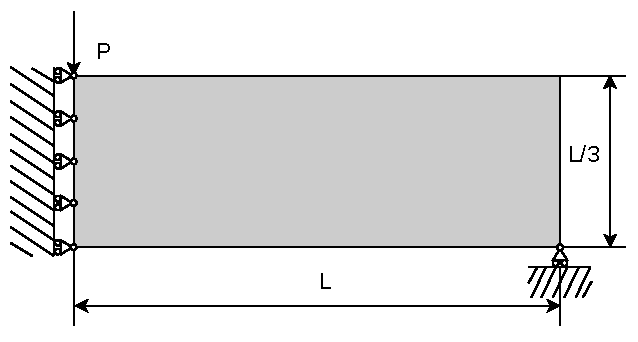
\includegraphics[width=0.90\linewidth,
						height=0.30\paperheight, keepaspectratio]{mbb_schematic}
					\end{center}
					
					\vspace{-8pt}
					
					{\fontsize{7.5}{11}\selectfont\sffamily
						左侧对称边界，右下滑移支撑，左上施加竖向点载荷；参数取 $P=1\,\mathrm{N}$；%
						$E=1\,\mathrm{MPa},\; \nu=0.3,\; V_f=0.5$。}
					
				\end{tcolorbox}
			\end{column}
			
		\end{columns}
		
	\end{frame}
	
	% ============================================================
	%  03-5  不同离散方式与密度表征的比较
	% ============================================================
	
	\begin{frame}
		\frametitle{不同离散方式与密度表征的比较}
		
		% ── 顶部总述条：随 overlay 切换 ──────────────────────────
		\begin{tcolorbox}[
			colback=panelbg, colframe=structure.fg!40,
			arc=3pt, boxrule=0.5pt,
			top=3pt, bottom=3pt, left=8pt, right=8pt]
			\only<1>{%
				\tcbox[on line, arc=3pt,
				colback=structure.fg, colframe=structure.fg,
				boxrule=0pt,
				top=1pt, bottom=1pt, left=5pt, right=5pt,
				fontupper=\fontsize{7}{9}\selectfont\bfseries\sffamily\color{white}]
				{比较维度 01：有限元离散阶次}%
				\quad
				{\fontsize{8}{12}\selectfont\sffamily
					以二维对称 MBB 梁为基准算例，在统一四边形单元、体积约束与优化参数下，比较无过滤情形中
					不同有限元阶次对优化结果的影响。}}%
			\only<2>{%
				\tcbox[on line, arc=3pt,
				colback=structure.fg, colframe=structure.fg,
				boxrule=0pt,
				top=1pt, bottom=1pt, left=5pt, right=5pt,
				fontupper=\fontsize{7}{9}\selectfont\bfseries\sffamily\color{white}]
				{比较维度 02：设计变量表征方式}%
				\quad
				{\fontsize{8}{12}\selectfont\sffamily
					在同一基准算例下，固定四边形单元、有限元阶次 $k = 2$ 与灵敏度过滤半径，
					比较单元密度与节点密度表征对优化结果的影响。}}%
			\only<3>{%
				\tcbox[on line, arc=3pt,
				colback=structure.fg, colframe=structure.fg,
				boxrule=0pt,
				top=1pt, bottom=1pt, left=5pt, right=5pt,
				fontupper=\fontsize{7}{9}\selectfont\bfseries\sffamily\color{white}]
				{比较维度 03：单元类型适用性}%
				\quad
				{\fontsize{8}{12}\selectfont\sffamily
					在同一基准算例下，固定有限元阶次 $k = 2$ 与灵敏度过滤半径，
					进一步考察三角形单元中不同密度表征方式的优化结果。}}%
		\end{tcolorbox}
		
		\vspace{-1.0em}
		
		% ── 主体内容区：overlayarea 锁高 ─────────────────────────
		\begin{overlayarea}{\linewidth}{0.50\paperheight}
			
			% ── Overlay 1：有限元离散阶次比较 ────────────────────
			\only<1>{%
				\begin{columns}[T, totalwidth=\linewidth]
					
					\begin{column}{0.325\linewidth}
						\begin{tcolorbox}[
							colback=white, colframe=structure.fg!50,
							colbacktitle=structure.fg, coltitle=white,
							fonttitle=\fontsize{8}{10}\selectfont\bfseries\sffamily,
							title={\circnum{01}\enspace 线性元 \enspace $k = 1$},
							arc=3pt, boxrule=0.5pt,
							toptitle=0.25pt, bottomtitle=0.25pt,
							top=5pt, bottom=5pt, left=5pt, right=5pt]
							\begin{center}
								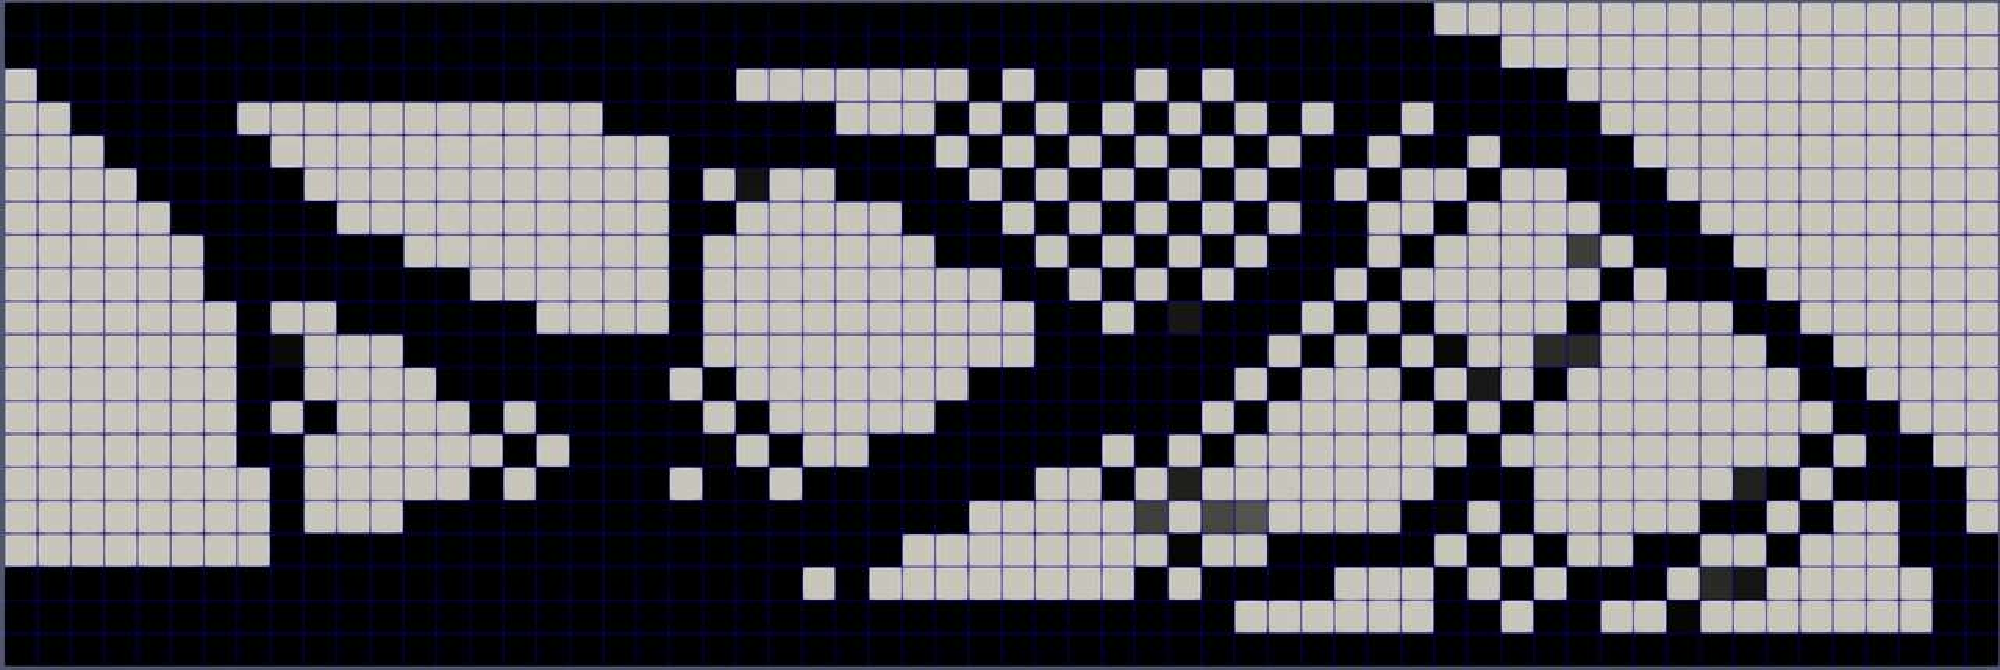
\includegraphics[width=\linewidth,
								height=0.30\paperheight, keepaspectratio]{topo_k1}
							\end{center}
							{\fontsize{7.5}{11}\selectfont\sffamily\centering\par
								$n = 53$,  $c \approx 203.07$\\
								棋盘格现象明显，边界锯齿化突出}
						\end{tcolorbox}
					\end{column}
					
					\begin{column}{0.325\linewidth}
						\begin{tcolorbox}[
							colback=white, colframe=structure.fg!50,
							colbacktitle=structure.fg, coltitle=white,
							fonttitle=\fontsize{8}{10}\selectfont\bfseries\sffamily,
							title={\circnum{02}\enspace 二阶元 \enspace $k = 2$},
							arc=3pt, boxrule=0.5pt,
							toptitle=0.25pt, bottomtitle=0.25pt,
							top=5pt, bottom=5pt, left=5pt, right=5pt]
							\begin{center}
								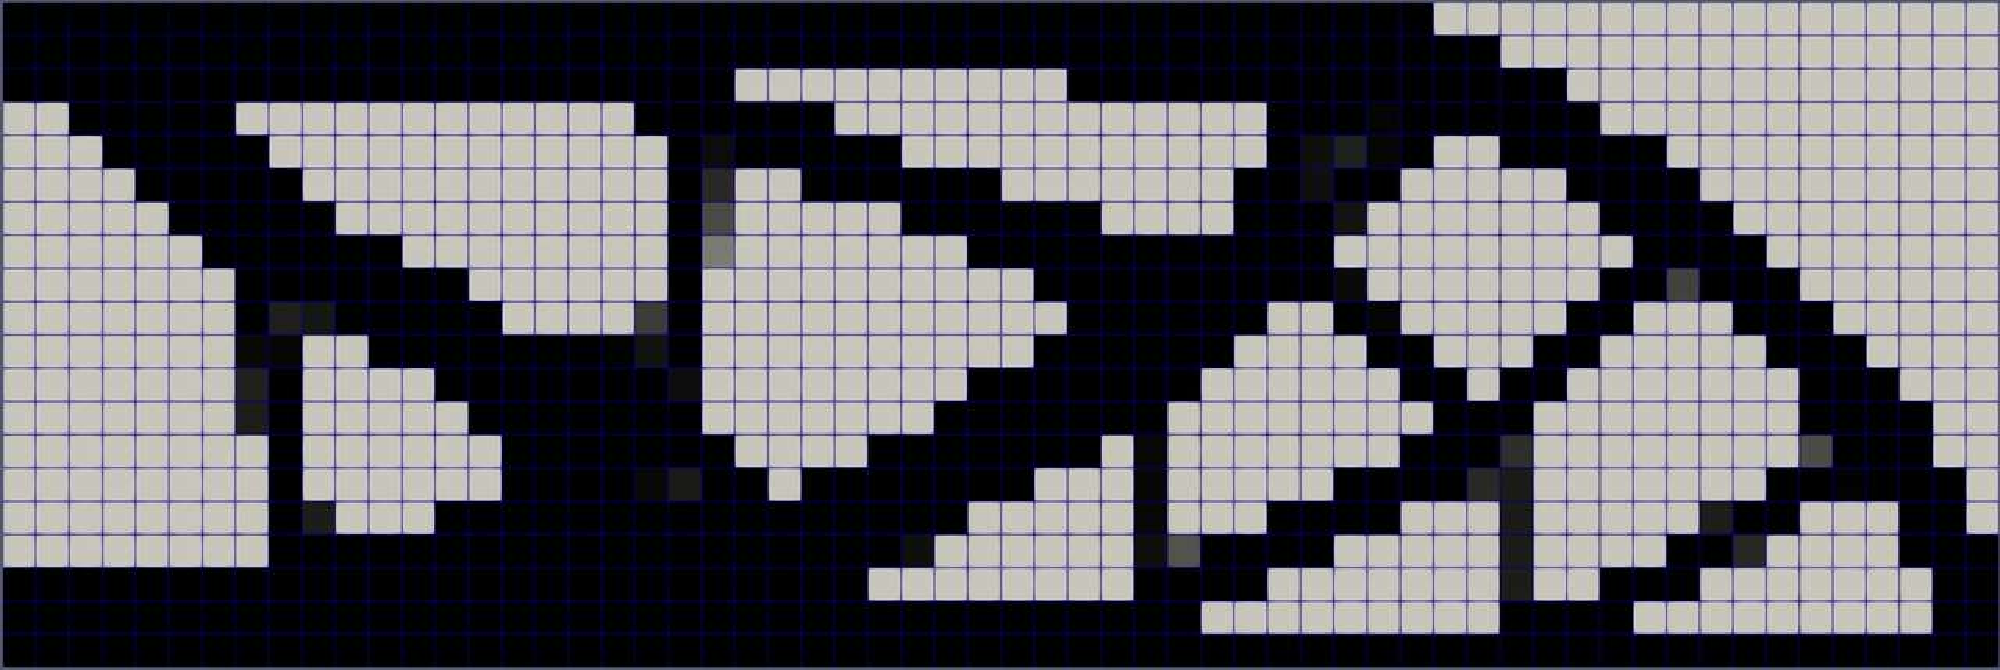
\includegraphics[width=\linewidth,
								height=0.30\paperheight, keepaspectratio]{topo_k2}
							\end{center}
							{\fontsize{7.5}{11}\selectfont\sffamily\centering\par
								$n = 36$,  $c \approx 213.18$\\
								构型质量明显改善，局部伪结构减少}
						\end{tcolorbox}
					\end{column}
					
					\begin{column}{0.325\linewidth}
						\begin{tcolorbox}[
							colback=white, colframe=structure.fg!50,
							colbacktitle=structure.fg, coltitle=white,
							fonttitle=\fontsize{8}{10}\selectfont\bfseries\sffamily,
							title={\circnum{03}\enspace 四阶元 \enspace $k = 4$},
							arc=3pt, boxrule=0.5pt,
							toptitle=0.25pt, bottomtitle=0.25pt,
							top=5pt, bottom=5pt, left=5pt, right=5pt]
							\begin{center}
								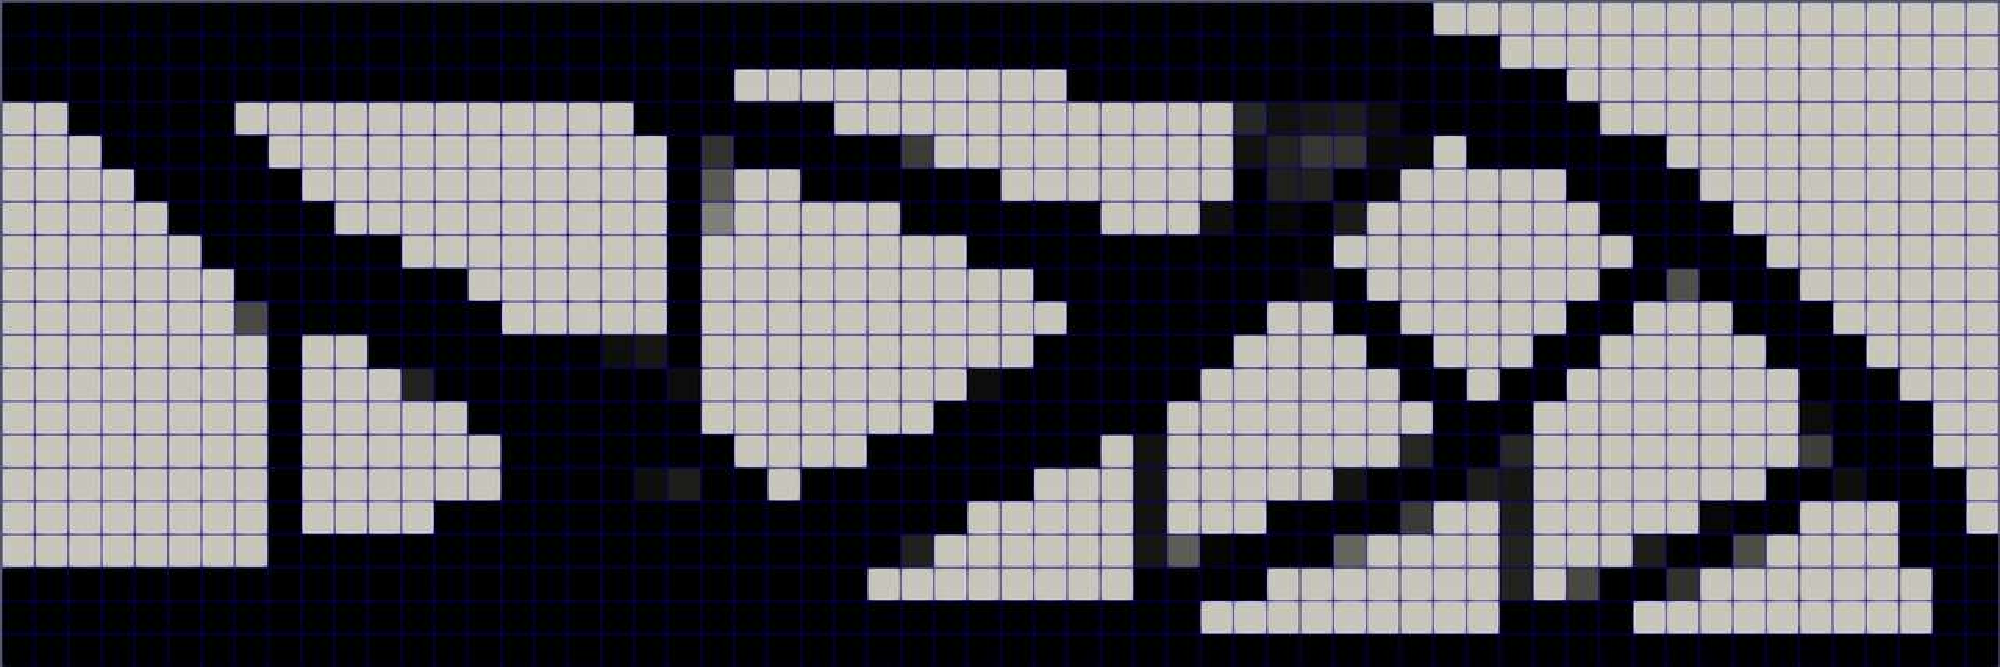
\includegraphics[width=\linewidth,
								height=0.30\paperheight, keepaspectratio]{topo_k4}
							\end{center}
							{\fontsize{7.5}{11}\selectfont\sffamily\centering\par
								$n = 41$,  $c \approx 218.66$\\
								相较 $k=2$ 改善有限，拓扑细节未同步提升}
						\end{tcolorbox}
					\end{column}
					
				\end{columns}
			}% end only<1>
			
			% ── Overlay 2：设计变量表征方式比较 ──────────────────────────
			\only<2>{%
				\begin{columns}[T, totalwidth=\linewidth]
					
					% ─── 01 单元密度表征 ─────────────────────────────
					\begin{column}{0.485\linewidth}
						\begin{tcolorbox}[
							colback=white, colframe=structure.fg!50,
							colbacktitle=structure.fg, coltitle=white,
							fonttitle=\fontsize{8}{10}\selectfont\bfseries\sffamily,
							title={\circnum{01}\enspace 单元密度表征},
							arc=3pt, boxrule=0.5pt,
							toptitle=0.25pt, bottomtitle=0.25pt,
							top=5pt, bottom=5pt, left=5pt, right=5pt,
							height=0.45\paperheight, valign=top]
							\begin{center}
								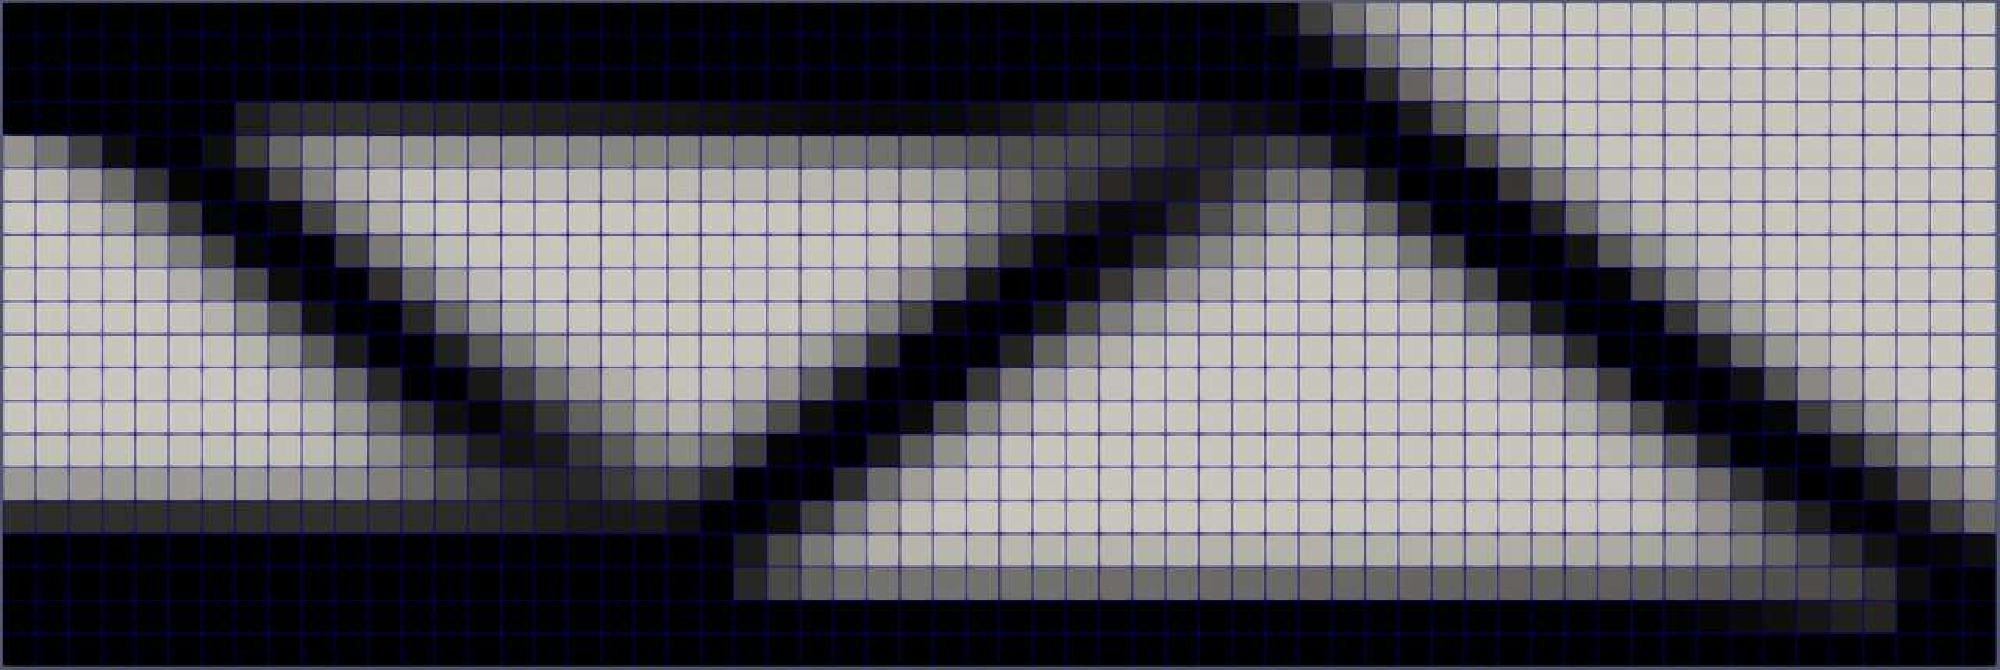
\includegraphics[width=0.85\linewidth,
								height=0.26\paperheight, keepaspectratio]{topo_elem_density}
							\end{center}
							\vspace{-6pt}
							{\fontsize{7.5}{11}\selectfont\sffamily\centering\par
								$n = 115$,  $c \approx 226.25$\\
								宏观拓扑稳定，收敛步数较少；
								但边界阶梯化特征相对明显}
						\end{tcolorbox}
					\end{column}
					
					% ─── 02 节点密度表征 ─────────────────────────────
					\begin{column}{0.485\linewidth}
						\begin{tcolorbox}[
							colback=white, colframe=structure.fg!50,
							colbacktitle=structure.fg, coltitle=white,
							fonttitle=\fontsize{8}{10}\selectfont\bfseries\sffamily,
							title={\circnum{02}\enspace 节点密度表征},
							arc=3pt, boxrule=0.5pt,
							toptitle=0.25pt, bottomtitle=0.25pt,
							top=5pt, bottom=5pt, left=5pt, right=5pt,
							height=0.45\paperheight, valign=top]
							\begin{center}
								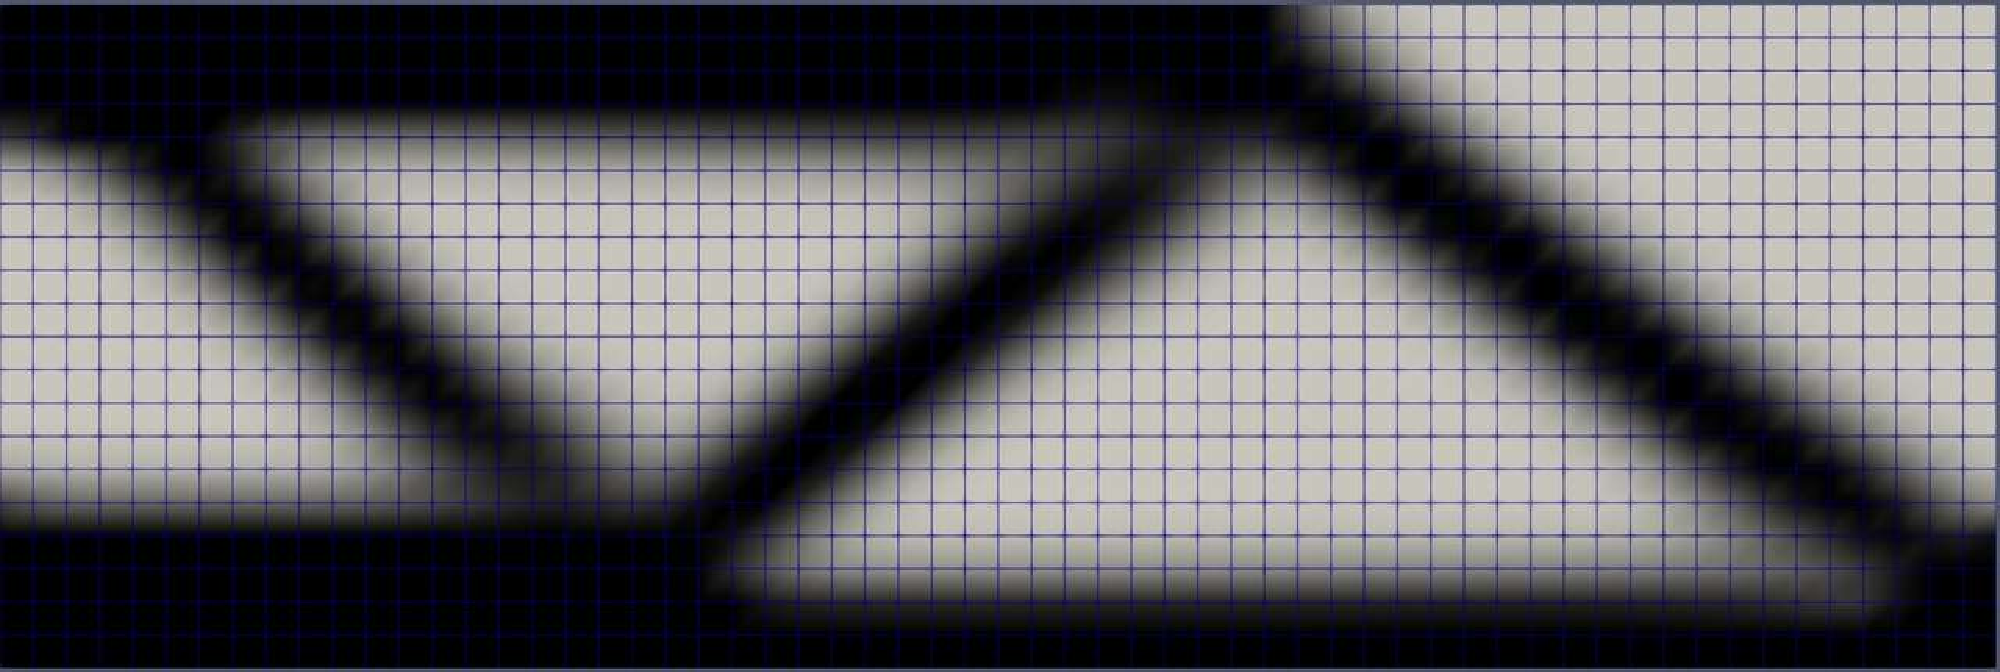
\includegraphics[width=0.85\linewidth,
								height=0.30\paperheight, keepaspectratio]{topo_node_density}
							\end{center}
							\vspace{-6pt}
							{\fontsize{7.5}{11}\selectfont\sffamily\centering\par
								$n = 144$, $c \approx 229.61$\\
								宏观拓扑基本一致，边界过渡更平滑；
								但收敛步数有所增加}
						\end{tcolorbox}
					\end{column}
					
				\end{columns}
			}% end only<2>
			
			% ── Overlay 3：综合认识 ───────────────────────────────
			\only<3>{%
				\begin{columns}[T, totalwidth=\linewidth]
					
					% ─── 01 三角形单元：单元密度表 ─────────────────────────────
					\begin{column}{0.485\linewidth}
						\begin{tcolorbox}[
							colback=white, colframe=structure.fg!50,
							colbacktitle=structure.fg, coltitle=white,
							fonttitle=\fontsize{8}{10}\selectfont\bfseries\sffamily,
							title={\circnum{01}\enspace 三角形单元：单元密度表征},
							arc=3pt, boxrule=0.5pt,
							toptitle=0.25pt, bottomtitle=0.25pt,
							top=5pt, bottom=5pt, left=5pt, right=5pt,
							height=0.45\paperheight, valign=top]
							\begin{center}
								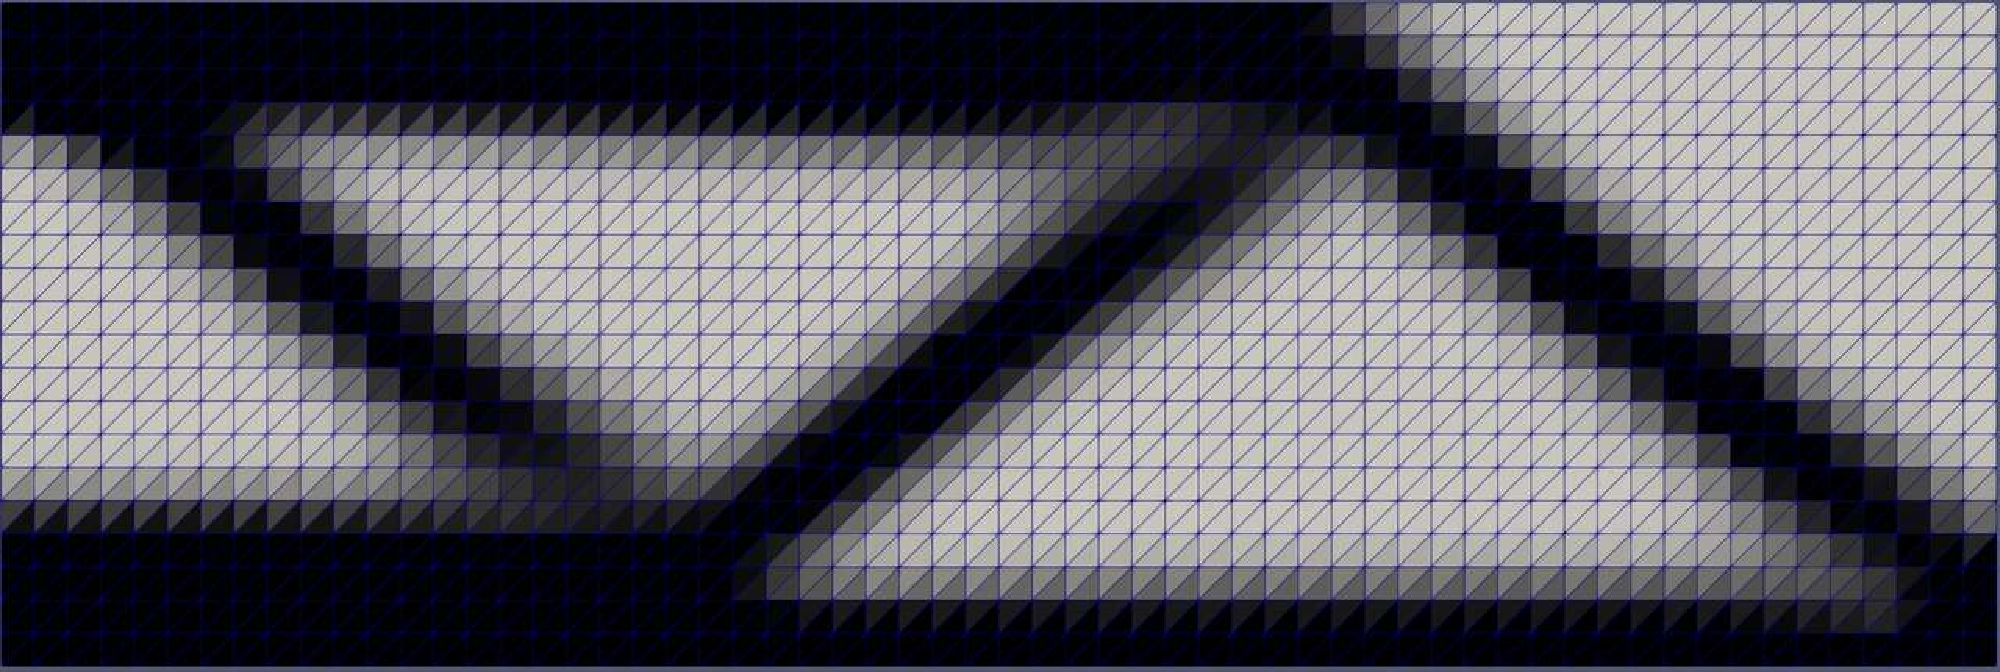
\includegraphics[width=0.85\linewidth,
								height=0.26\paperheight, keepaspectratio]{topo_tri_elem_density}
							\end{center}
							\vspace{-6pt}
							{\fontsize{7.5}{11}\selectfont\sffamily\centering\par
								$n = 98$,  $c \approx 224.21$\\
								在三角形网格上获得稳定主承载路径，
								说明单元密度表征可自然迁移至单纯形单元。}
						\end{tcolorbox}
					\end{column}
					
					% ─── 02 三角形单元：节点密度表征 ─────────────────────────────
					\begin{column}{0.485\linewidth}
						\begin{tcolorbox}[
							colback=white, colframe=structure.fg!50,
							colbacktitle=structure.fg, coltitle=white,
							fonttitle=\fontsize{8}{10}\selectfont\bfseries\sffamily,
							title={\circnum{02}\enspace 三角形单元：节点密度表征},
							arc=3pt, boxrule=0.5pt,
							toptitle=0.25pt, bottomtitle=0.25pt,
							top=5pt, bottom=5pt, left=5pt, right=5pt,
							height=0.45\paperheight, valign=top]
							\begin{center}
								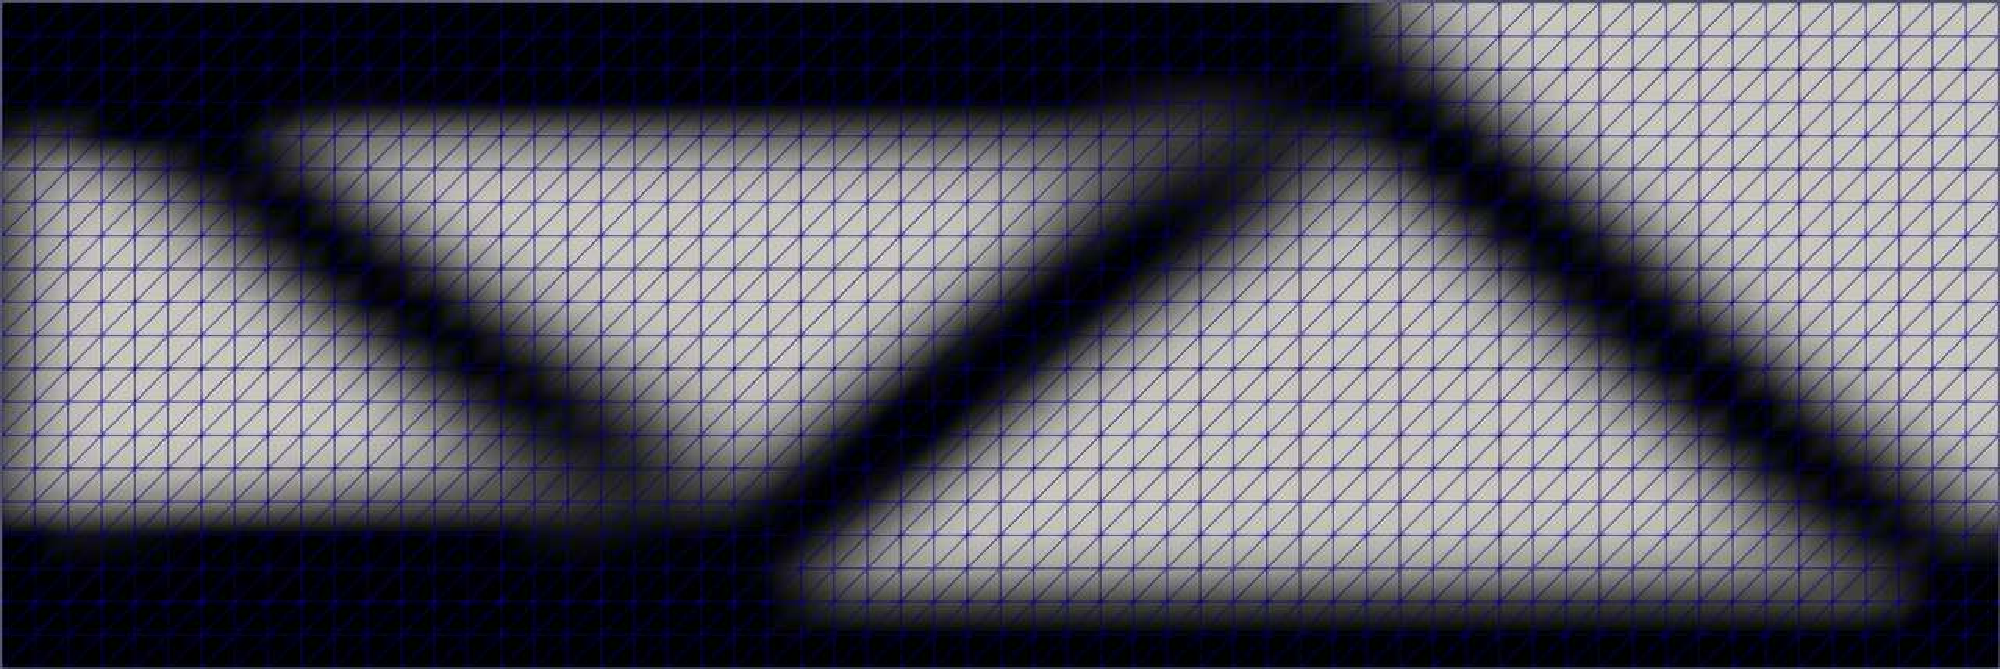
\includegraphics[width=0.85\linewidth,
								height=0.30\paperheight, keepaspectratio]{topo_tri_node_density}
							\end{center}
							\vspace{-6pt}
							{\fontsize{7.5}{11}\selectfont\sffamily\centering\par
								$n = 109$, $c \approx 228.93$\\
								节点密度场保持连续表征优势，主拓扑特征与单元密度结果一致。}
						\end{tcolorbox}
					\end{column}
					
				\end{columns}
			}% end only<3>
			
		\end{overlayarea}
		
		% ── 底部结论条：随 overlay 切换 ──────────────────────────
		\begin{tcolorbox}[
			colback=structure.fg, colframe=structure.fg,
			arc=3pt, boxrule=0pt,
			top=4pt, bottom=4pt, left=8pt, right=8pt]
			\centering
			{\fontsize{8.5}{12}\selectfont\sffamily\color{white}
				\only<1>{提高分析阶次具有一定改善作用，但其收益受单分辨率设计空间限制}%
				\only<2>{密度表征方式影响边界过渡与收敛行为，但不能突破单分辨率框架的设计分辨率限制}%
				\only<3>{统一框架可推广至三角形单元，支撑复杂几何与非结构网格拓扑优化}
			}
		\end{tcolorbox}
		
	\end{frame}
	
	% ============================================================
	%  03-6  应用推广：从基准结构到复杂算例
	% ============================================================
	
	\begin{frame}
		\frametitle{应用推广：从基准结构到复杂算例}
		
		% ── 顶部总述条：随 overlay 切换 ──────────────────────────
		\begin{tcolorbox}[
			colback=panelbg, colframe=structure.fg!40,
			arc=3pt, boxrule=0.5pt,
			top=3pt, bottom=3pt, left=8pt, right=8pt]
			\only<1>{%
				\tcbox[on line, arc=3pt,
				colback=structure.fg, colframe=structure.fg,
				boxrule=0pt,
				top=1pt, bottom=1pt, left=5pt, right=5pt,
				fontupper=\fontsize{7}{9}\selectfont\bfseries\sffamily\color{white}]
				{应用场景 01：二维简支桥梁}%
				\quad
				{\fontsize{8}{12}\selectfont\sffamily
					在典型桥梁受力场景下，检验任意次拉格朗日有限元拓扑优化框架的适用性。}}%
			\only<2>{%
				\tcbox[on line, arc=3pt,
				colback=structure.fg, colframe=structure.fg,
				boxrule=0pt,
				top=1pt, bottom=1pt, left=5pt, right=5pt,
				fontupper=\fontsize{7}{9}\selectfont\bfseries\sffamily\color{white}]
				{应用场景 02：三维悬臂梁}%
				\quad
				{\fontsize{8}{12}\selectfont\sffamily
					将二维拓扑优化框架推广到三维结构问题，检验高阶离散与密度表征在三维情形下的有效性。}}%
			\only<3>{%
				\tcbox[on line, arc=3pt,
				colback=structure.fg, colframe=structure.fg,
				boxrule=0pt,
				top=1pt, bottom=1pt, left=5pt, right=5pt,
				fontupper=\fontsize{7}{9}\selectfont\bfseries\sffamily\color{white}]
				{应用场景 03：位移反向器}%
				\quad
				{\fontsize{8}{12}\selectfont\sffamily
					由柔顺度最小化推广到柔顺机构设计，验证该离散框架对非自伴随目标问题的适用性。}}%
		\end{tcolorbox}
		
		\vspace{-1.2em}
		
		% ── 主体内容区：锁定高度，防止 overlay 抖动 ───────────────
		\begin{overlayarea}{\linewidth}{0.52\paperheight}
			
			% ========================================================
			% Overlay 1：二维简支桥梁
			% ========================================================
			\only<1>{%
				\begin{columns}[T, totalwidth=\linewidth]
					
					% ─── 左栏：初始设计区 ─────────────────────────
					\begin{column}{0.485\linewidth}
						\begin{tcolorbox}[
							colback=white, colframe=structure.fg!50,
							colbacktitle=structure.fg, coltitle=white,
							fonttitle=\fontsize{8}{10}\selectfont\bfseries\sffamily,
							title={\circnum{01}\enspace 初始设计域与边界载荷},
							arc=3pt, boxrule=0.5pt,
							toptitle=0.25pt, bottomtitle=0.25pt,
							top=5pt, bottom=5pt, left=5pt, right=5pt,
							height=0.48\paperheight, valign=top]
							
							\vspace{-0.6em}
							
							% 固定高度图像区：保证左右两栏图片高度基线一致
							\begin{center}
								\begin{minipage}[c][0.285\paperheight][c]{0.96\linewidth}
									\centering
									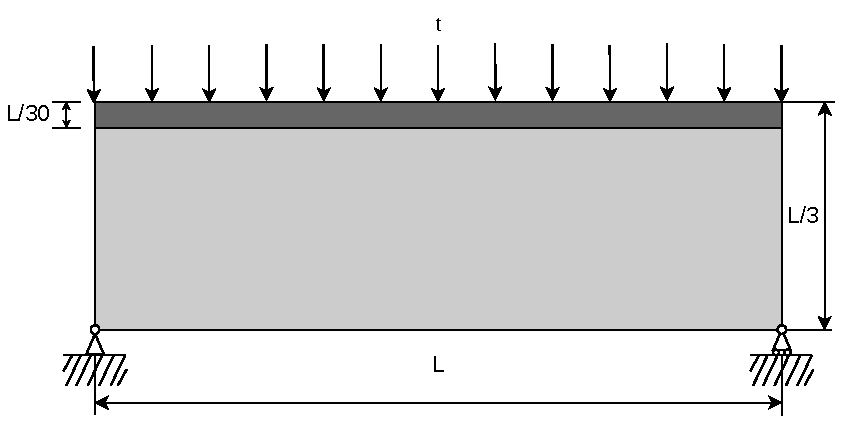
\includegraphics[
									width=0.92\linewidth,
									height=0.26\paperheight,
									keepaspectratio]{bridge2d_domain}
								\end{minipage}
							\end{center}
							
							\vspace{-0.8em}
							
							{\fontsize{7.2}{10.2}\selectfont\sffamily
								顶部非设计域、均布载荷与简支约束。相较 MBB 梁，更适合检验复杂约束下的适用性。
							}
						\end{tcolorbox}
					\end{column}
					
					% ─── 右栏：代表性收敛结果 ─────────────────────
					\begin{column}{0.485\linewidth}
						\begin{tcolorbox}[
							colback=white, colframe=structure.fg!50,
							colbacktitle=structure.fg, coltitle=white,
							fonttitle=\fontsize{8}{10}\selectfont\bfseries\sffamily,
							title={\circnum{02}\enspace 代表性收敛结果},
							arc=3pt, boxrule=0.5pt,
							toptitle=0.25pt, bottomtitle=0.25pt,
							top=5pt, bottom=5pt, left=5pt, right=5pt,
							height=0.48\paperheight, valign=top]
							
							\vspace{-0.6em}
							
							% 固定高度图像区：与左栏保持一致
							\begin{center}
								\begin{minipage}[c][0.285\paperheight][c]{0.96\linewidth}
									\centering
									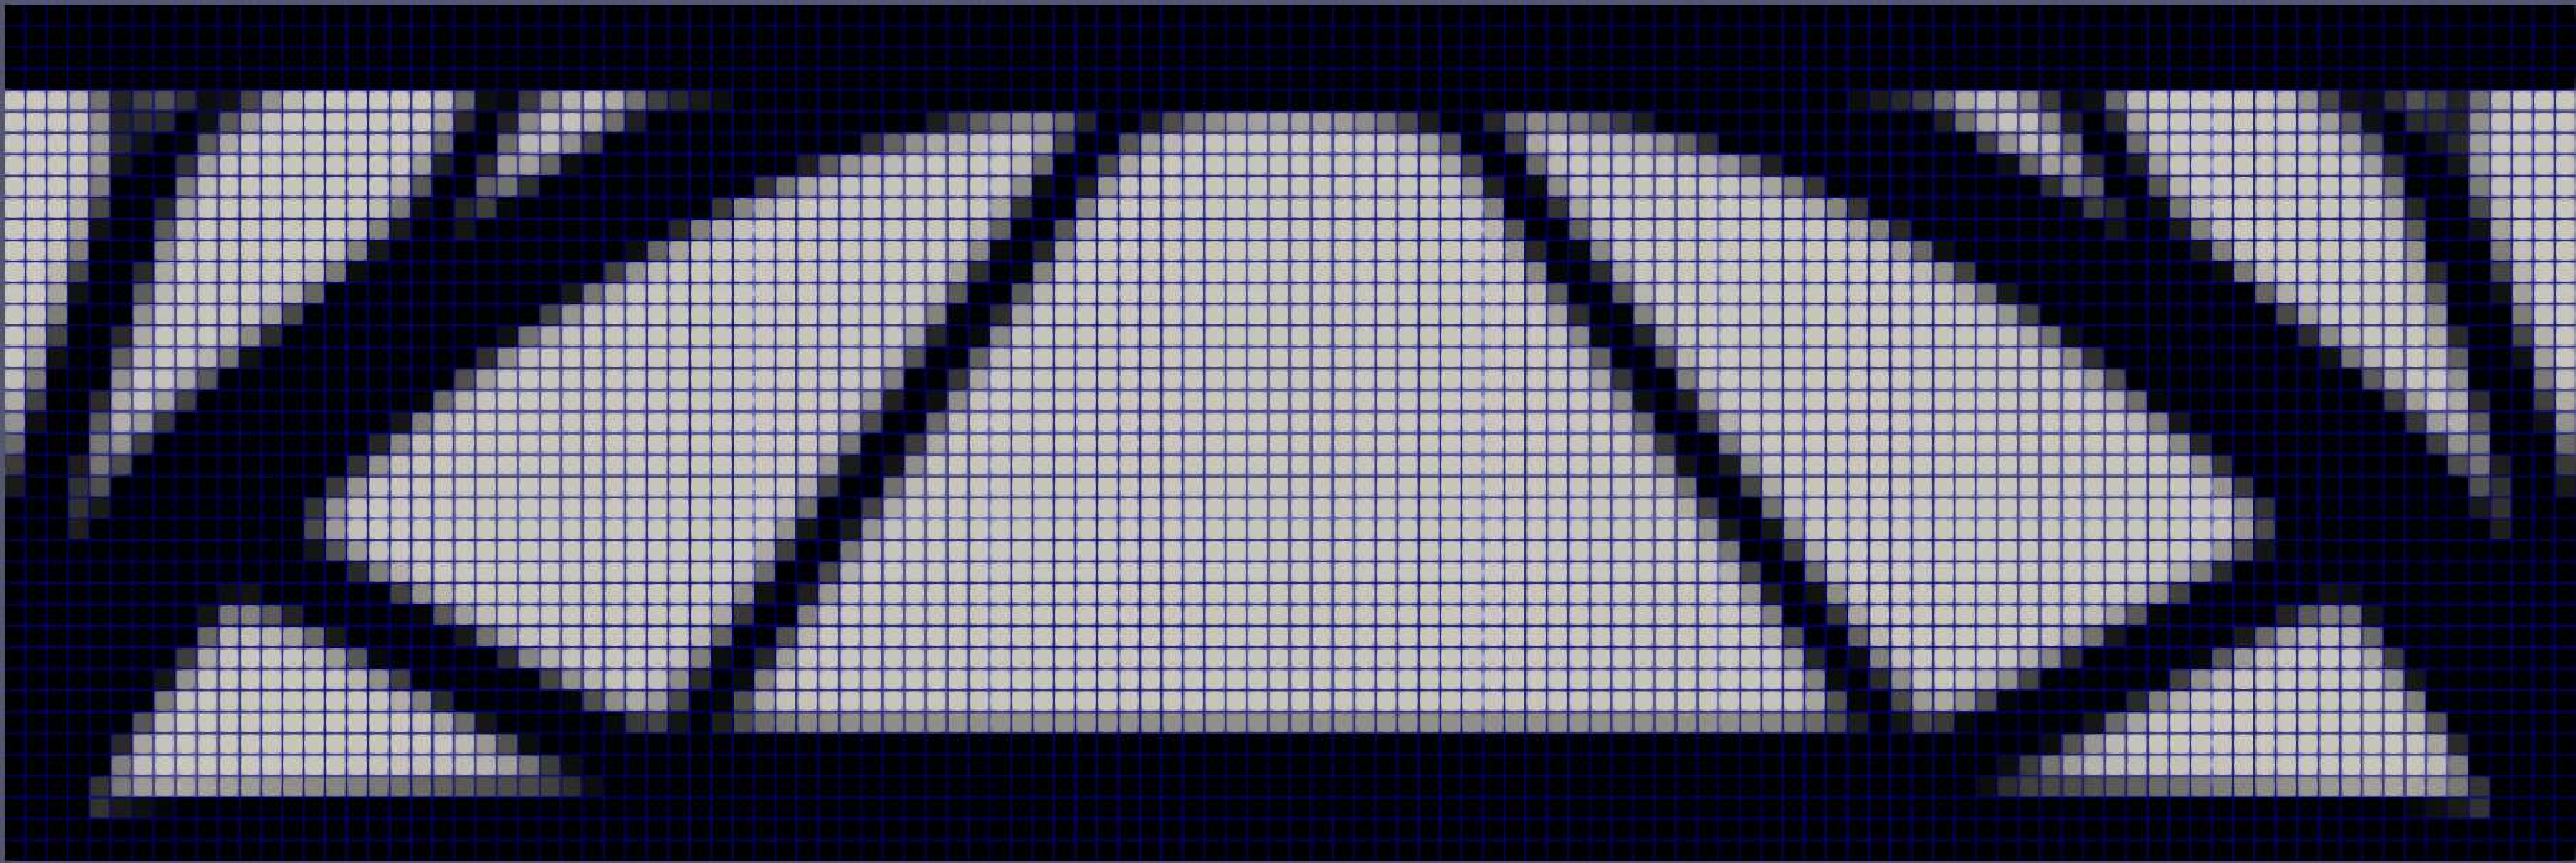
\includegraphics[
									width=0.92\linewidth,
									height=0.26\paperheight,
									keepaspectratio]{bridge2d_result}
								\end{minipage}
							\end{center}
							
							\vspace{-0.8em}
							
							{\fontsize{7.2}{10.2}\selectfont\sffamily
								形成“桥面--拱形支撑--腹杆”传力路径，拓扑构型与简支桥梁受力机制保持一致。
							}
						\end{tcolorbox}
					\end{column}
					
				\end{columns}
			}
			
			% ========================================================
			% Overlay 2：三维悬臂梁
			% ========================================================
			\only<2>{%
				\begin{columns}[T, totalwidth=\linewidth]
					
					% ─── 左栏：初始设计区 ─────────────────────────
					\begin{column}{0.485\linewidth}
						\begin{tcolorbox}[
							colback=white, colframe=structure.fg!50,
							colbacktitle=structure.fg, coltitle=white,
							fonttitle=\fontsize{8}{10}\selectfont\bfseries\sffamily,
							title={\circnum{01}\enspace 初始三维设计域},
							arc=3pt, boxrule=0.5pt,
							toptitle=0.25pt, bottomtitle=0.25pt,
							top=5pt, bottom=5pt, left=5pt, right=5pt,
							height=0.48\paperheight, valign=top]
							
							\vspace{-0.6em}
							
							\begin{center}
								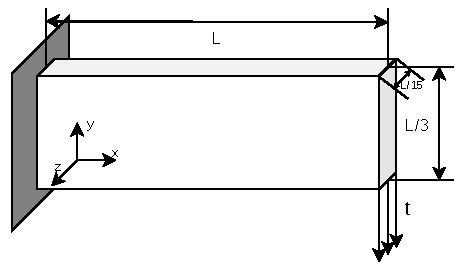
\includegraphics[
								width=0.92\linewidth,
								height=0.28\paperheight,
								keepaspectratio]{cantilever3d_domain}
							\end{center}
							
							\vspace{-1.0em}
							
							{\fontsize{7.3}{10.5}\selectfont\sffamily
								在厚度方向引入有限尺寸，二维问题自然推广至三维应力状态与空间构件布置。}
						\end{tcolorbox}
					\end{column}
					
					% ─── 右栏：代表性收敛结果 ─────────────────────
					\begin{column}{0.485\linewidth}
						\begin{tcolorbox}[
							colback=white, colframe=structure.fg!50,
							colbacktitle=structure.fg, coltitle=white,
							fonttitle=\fontsize{8}{10}\selectfont\bfseries\sffamily,
							title={\circnum{02}\enspace 代表性收敛结果},
							arc=3pt, boxrule=0.5pt,
							toptitle=0.25pt, bottomtitle=0.25pt,
							top=5pt, bottom=5pt, left=5pt, right=5pt,
							height=0.48\paperheight, valign=top]
							
							\vspace{-0.3em}
							
							\begin{center}
								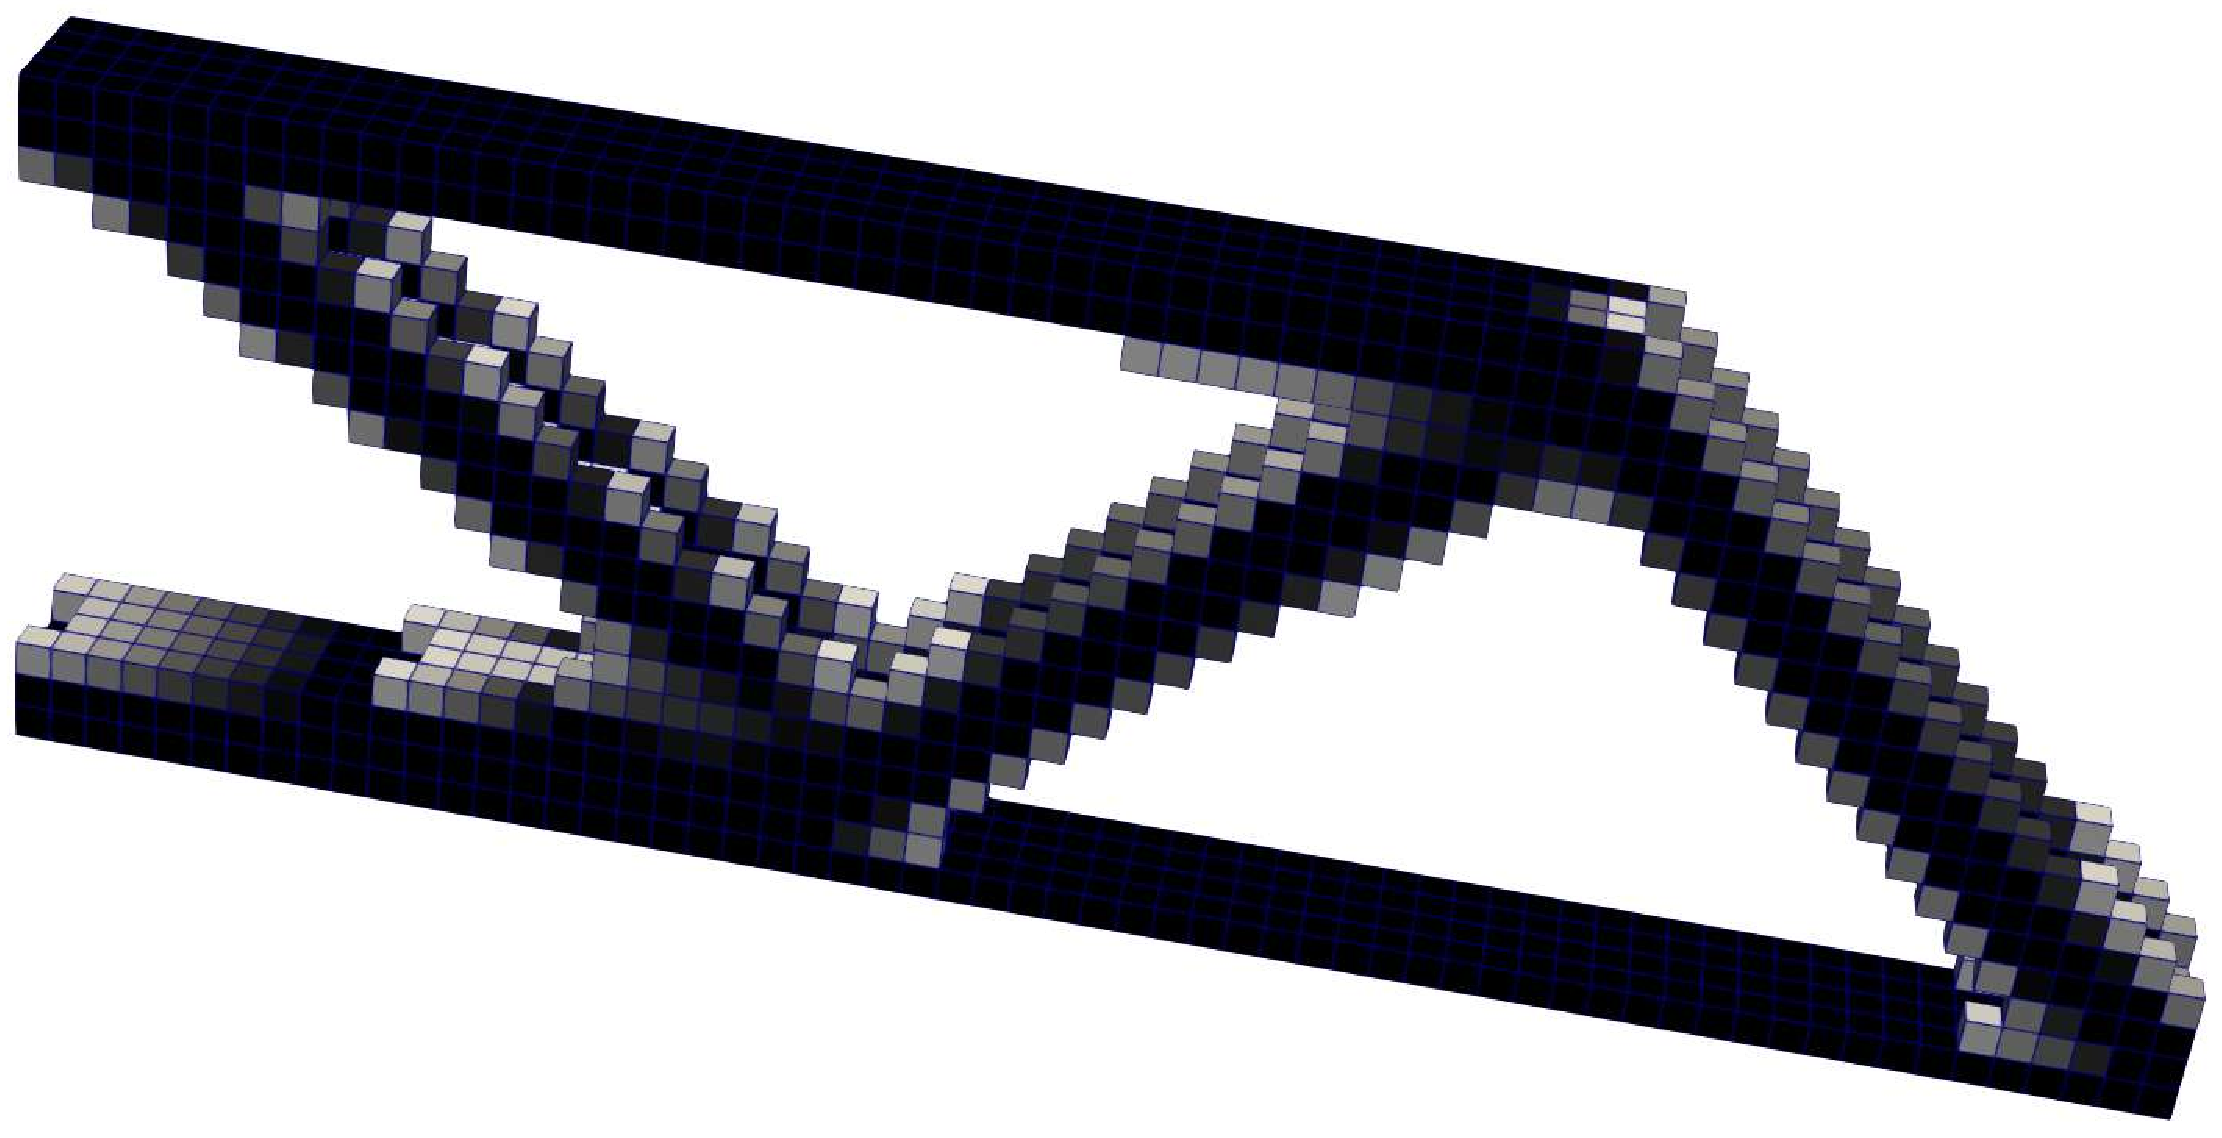
\includegraphics[
								width=0.92\linewidth,
								height=0.28\paperheight,
								keepaspectratio]{cantilever3d_result}
							\end{center}
							
							\vspace{-0.8em}
							
							{\fontsize{7.3}{10.5}\selectfont\sffamily
								获得清晰的三维空间承载路径，体现拓扑构型的受力特征。}
						\end{tcolorbox}
					\end{column}
					
				\end{columns}
			}
			
			% ========================================================
			% Overlay 3：位移反向器
			% ========================================================
			\only<3>{%
				\begin{columns}[T, totalwidth=\linewidth]
					
					% ─── 左栏：初始设计区 ─────────────────────────
					\begin{column}{0.485\linewidth}
						\begin{tcolorbox}[
							colback=white, colframe=structure.fg!50,
							colbacktitle=structure.fg, coltitle=white,
							fonttitle=\fontsize{8}{10}\selectfont\bfseries\sffamily,
							title={\circnum{01}\enspace 初始设计区与输入/输出端},
							arc=3pt, boxrule=0.5pt,
							toptitle=0.25pt, bottomtitle=0.25pt,
							top=5pt, bottom=5pt, left=5pt, right=5pt,
							height=0.48\paperheight, valign=top]
							
							\vspace{-0.6em}
							
							\begin{center}
								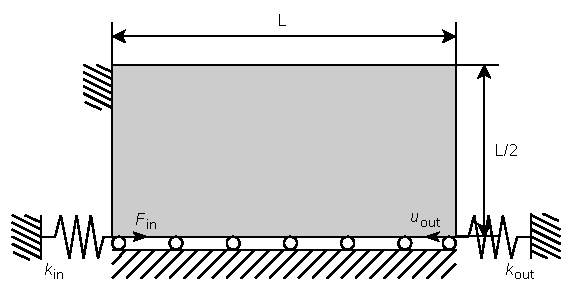
\includegraphics[
								width=0.92\linewidth,
								height=0.28\paperheight,
								keepaspectratio]{inverter_domain}
							\end{center}
							
							\vspace{-1.0em}
							
							{\fontsize{7.3}{10.5}\selectfont\sffamily
								输入端载荷与输出端位移目标定义机构，优化目标转向指定输出端位移最大化。}
						\end{tcolorbox}
					\end{column}
					
					% ─── 右栏：代表性收敛结果 ─────────────────────
					\begin{column}{0.485\linewidth}
						\begin{tcolorbox}[
							colback=white, colframe=structure.fg!50,
							colbacktitle=structure.fg, coltitle=white,
							fonttitle=\fontsize{8}{10}\selectfont\bfseries\sffamily,
							title={\circnum{02}\enspace 代表性收敛结果},
							arc=3pt, boxrule=0.5pt,
							toptitle=0.25pt, bottomtitle=0.25pt,
							top=5pt, bottom=5pt, left=5pt, right=5pt,
							height=0.48\paperheight, valign=top]
							
							\vspace{-0.3em}
							
							\begin{center}
								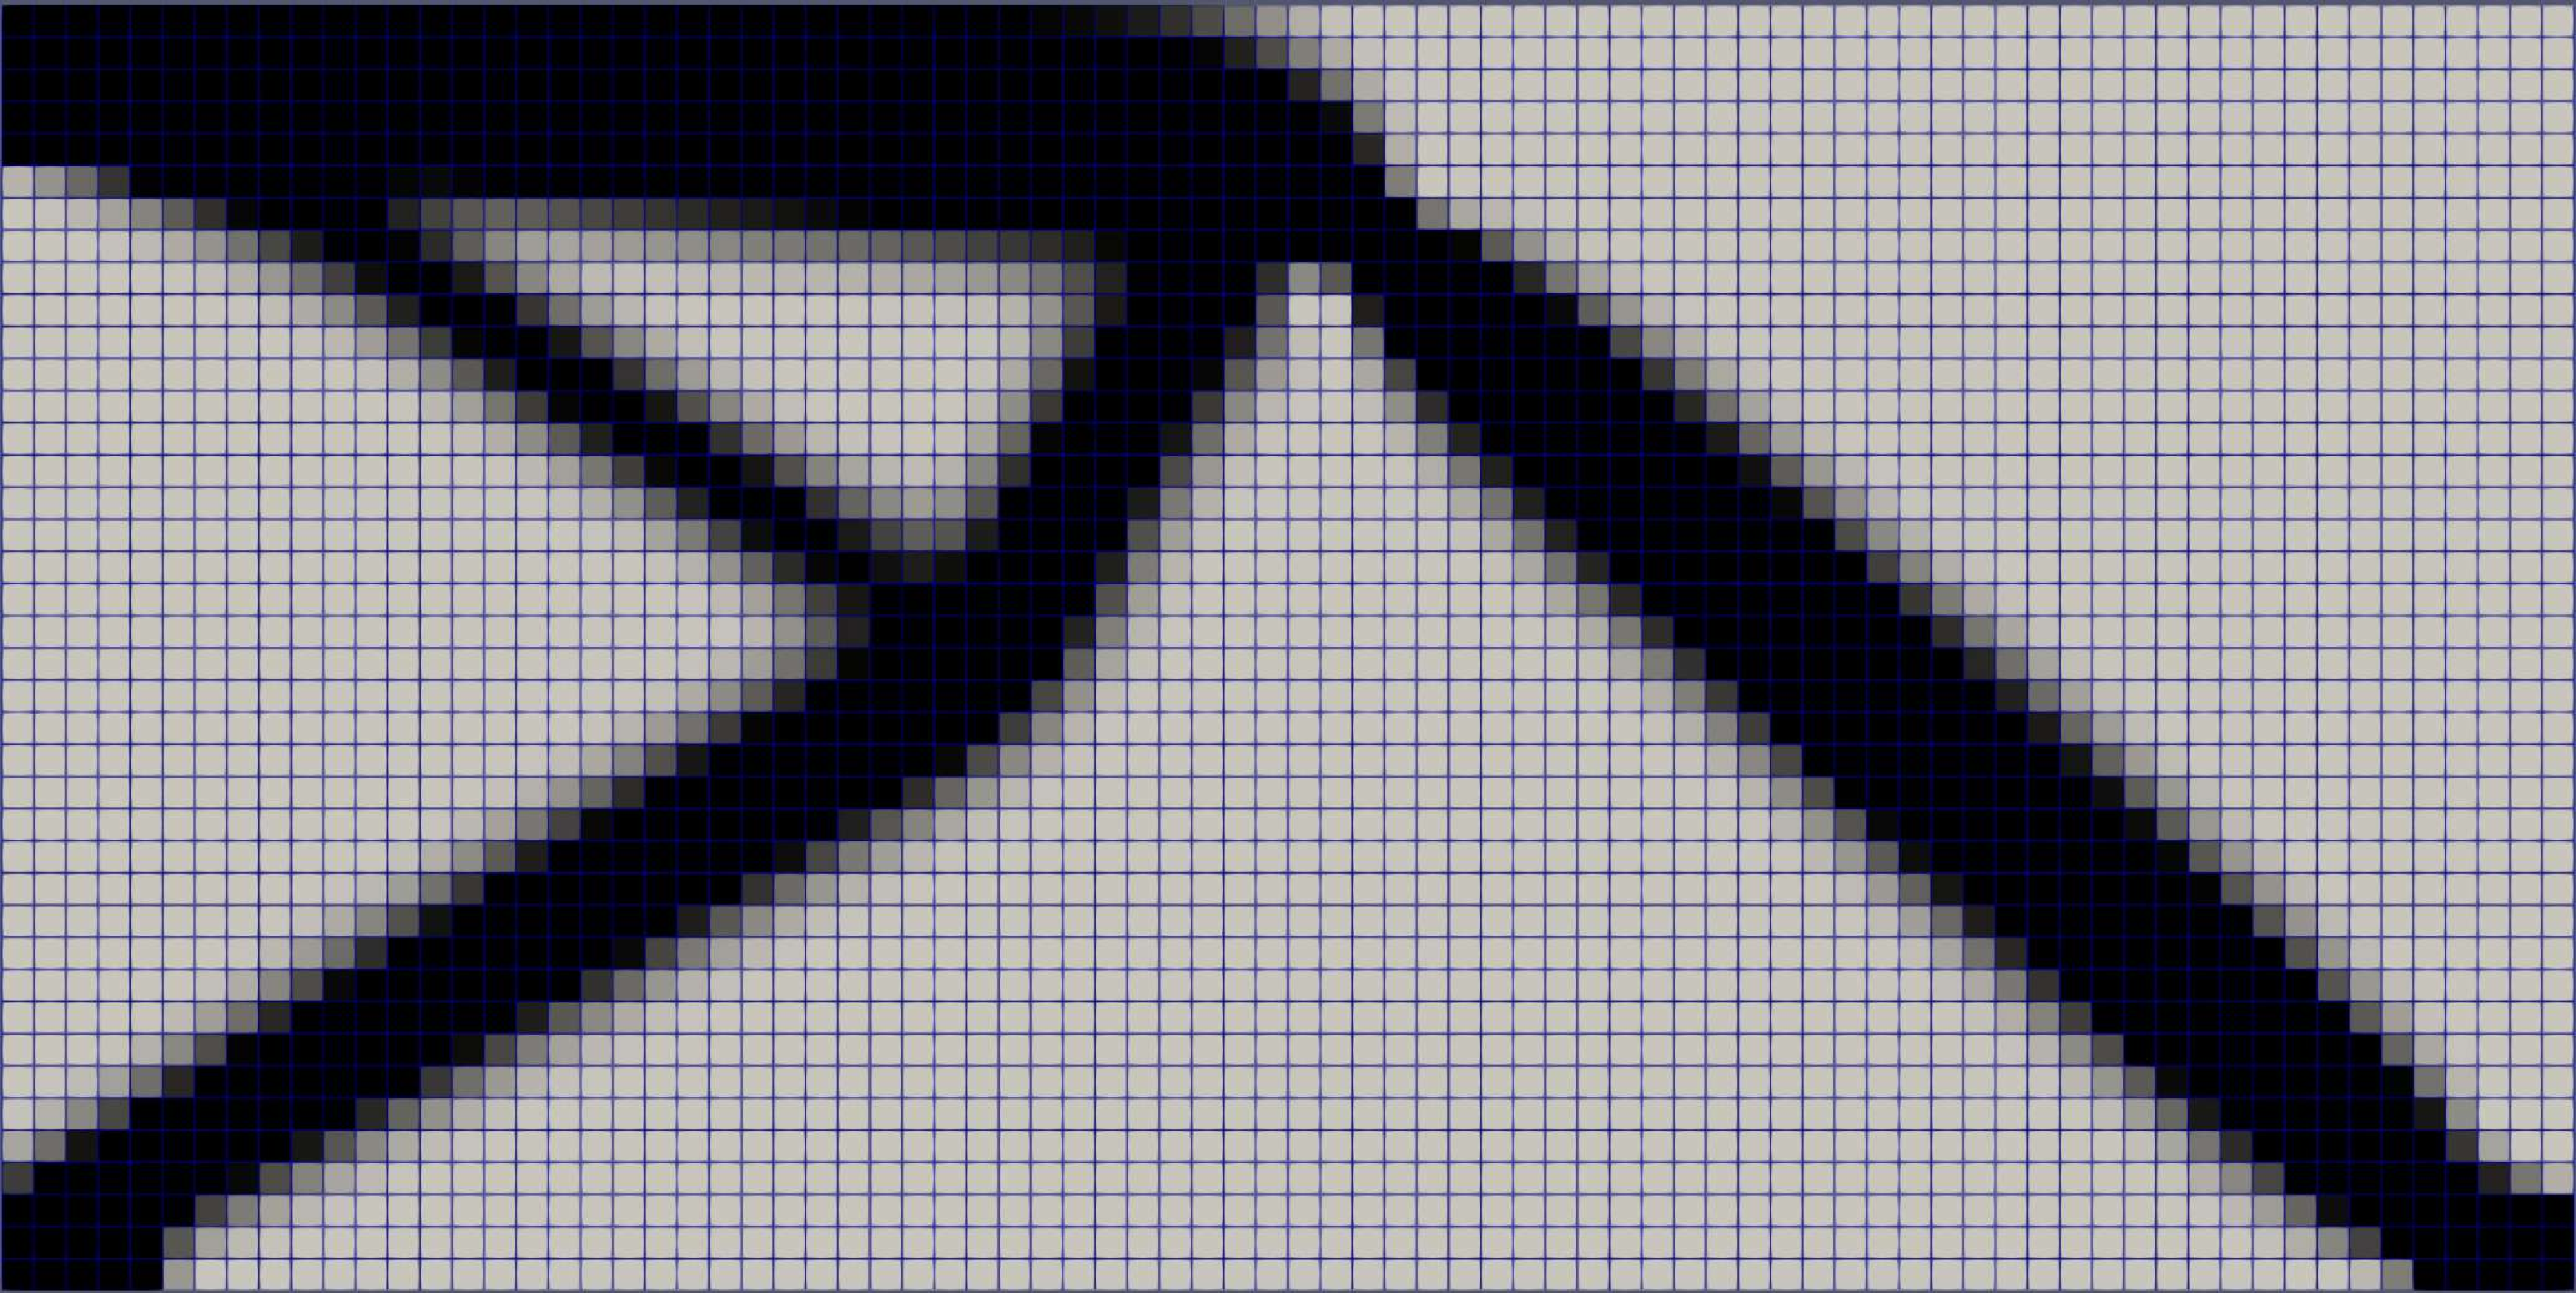
\includegraphics[
								width=0.90\linewidth,
								height=0.24\paperheight,
								keepaspectratio]{inverter_result}
							\end{center}
							
							\vspace{-0.8em}
							
							{\fontsize{7.3}{10.5}\selectfont\sffamily
								优化构型实现输入–输出位移方向转换，可推广至柔顺机构设计。}
						\end{tcolorbox}
					\end{column}
					
				\end{columns}
			}
			
		\end{overlayarea}
		
		% ── 底部结论条：随 overlay 切换 ──────────────────────────
		\begin{tcolorbox}[
			colback=structure.fg, colframe=structure.fg,
			arc=3pt, boxrule=0pt,
			top=4pt, bottom=4pt, left=8pt, right=8pt]
			\centering
			{\fontsize{8.4}{12}\selectfont\sffamily\color{white}
				\only<1>{二维简支桥梁算例验证了方法在复杂载荷与非设计域约束下的适用性}%
				\only<2>{三维悬臂梁算例表明该框架可从二维问题自然推广至三维结构拓扑优化}%
				\only<3>{位移反向器算例说明该框架不仅适用于刚度优化，也可服务于柔顺机构设计}%
			}
		\end{tcolorbox}
		
	\end{frame}
	
	
	% ============================================================
	\section{高精度的多分辨率拓扑优化架构}
	% ============================================================
	
	% ============================================================
	%  04-1  单分辨率框架的精度错配
	% ============================================================
	
	\begin{frame}
		\frametitle{单分辨率框架的精度错配}
		
		% ── 引导语 ───────────────────────────────────────────────
		\begin{tcolorbox}[
			colback=structure.fg!8, colframe=structure.fg!40,
			arc=2pt, boxrule=0.4pt,
			top=3pt, bottom=3pt, left=8pt, right=8pt]
			{\fontsize{8}{11}\selectfont\sffamily
				以二维对称 MBB 梁为例，考察单分辨率框架下分析精度与设计分辨率单侧提升导致的精度错配现象。}
		\end{tcolorbox}
		
		\vspace{-1.5em}
		
		% ── 主体三栏：基准 / 仅提分析精度 / 仅提设计分辨率 ───────
		\begin{columns}[T, totalwidth=\linewidth]
			
			% ─── 第一栏：基准情形 ─────────────────────────────
			\begin{column}{0.32\linewidth}
				\begin{tcolorbox}[
					colback=white, colframe=structure.fg!50,
					colbacktitle=structure.fg, coltitle=white,
					fonttitle=\fontsize{7.5}{10}\selectfont\bfseries\sffamily,
					title={\begin{minipage}[c][3.0em][c]{\linewidth}%
							\circnum{01}\enspace 基准情形:单分辨率框架，$k=2$%
					\end{minipage}},
					arc=3pt, boxrule=0.5pt,
					toptitle=0.25pt, bottomtitle=0.25pt,
					top=4pt, bottom=4pt, left=5pt, right=5pt,
					valign=top]
					\begin{center}
						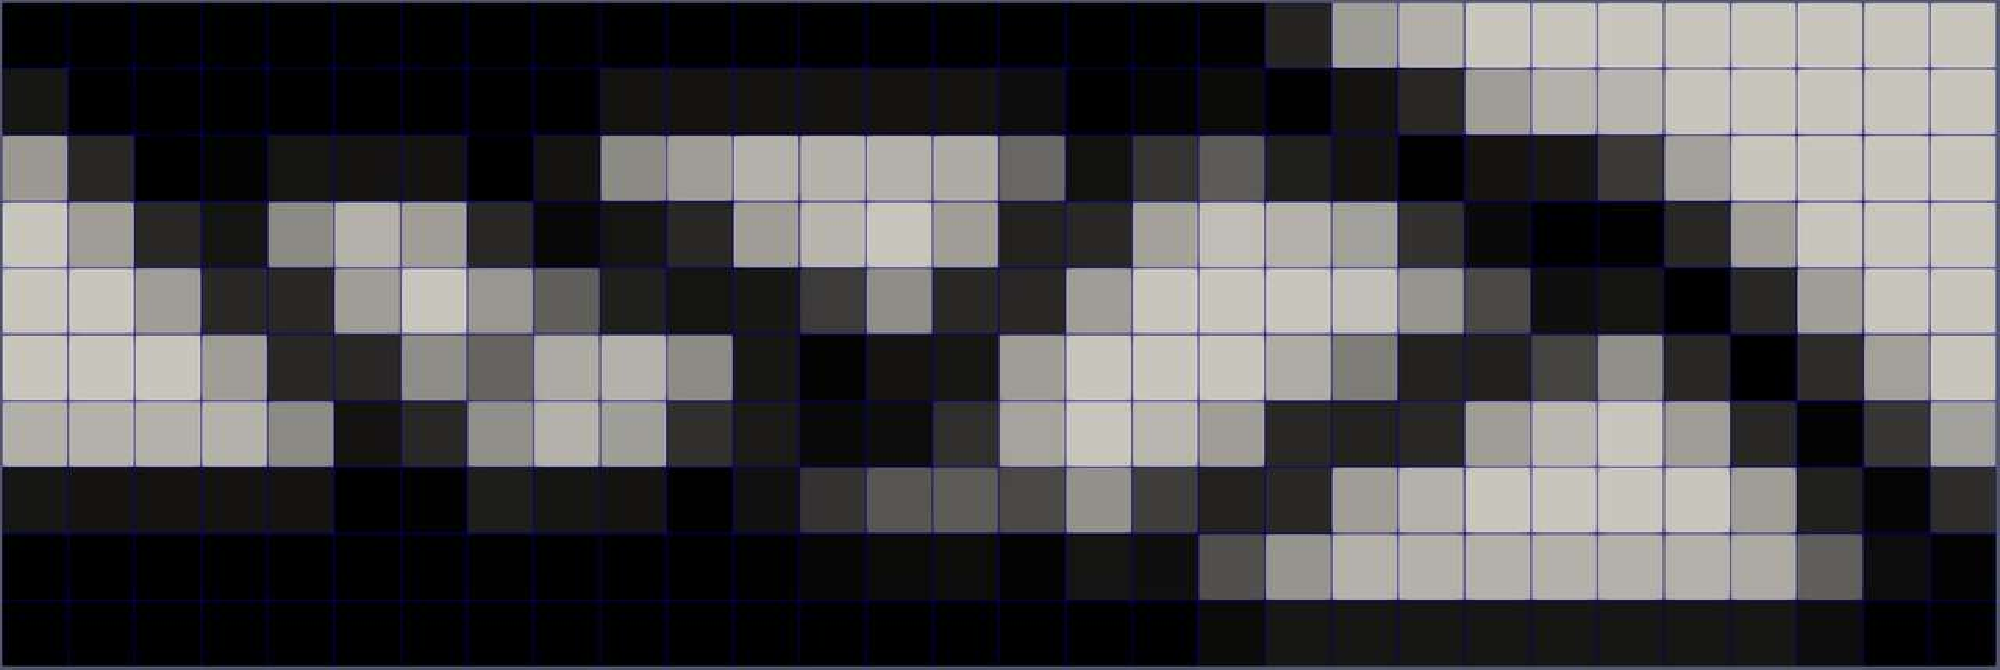
\includegraphics[width=0.92\linewidth,
						height=0.22\paperheight, keepaspectratio]{topo_baseline_k2}
					\end{center}
					{\fontsize{7}{10.5}\selectfont\sffamily\centering\par
						$\rho_{\mathrm{dof}} = 300,u_{\mathrm{dof}} = 2562$ \\[3pt]
						设计变量与分析单元绑定，限制拓扑表达分辨率}
				\end{tcolorbox}
			\end{column}
			
			% ─── 第二栏：仅提高分析精度 ───────────────────────
			\begin{column}{0.32\linewidth}
				\begin{tcolorbox}[
					colback=white, colframe=structure.fg!50,
					colbacktitle=structure.fg, coltitle=white,
					fonttitle=\fontsize{7.5}{10}\selectfont\bfseries\sffamily,
					title={\begin{minipage}[c][3.0em][c]{\linewidth}%
							\circnum{02}\enspace 仅提高分析精度：$k=2 \to 4$%
					\end{minipage}},
					arc=3pt, boxrule=0.5pt,
					toptitle=0.25pt, bottomtitle=0.25pt,
					top=4pt, bottom=4pt, left=5pt, right=5pt,
					valign=top]
					\begin{center}
						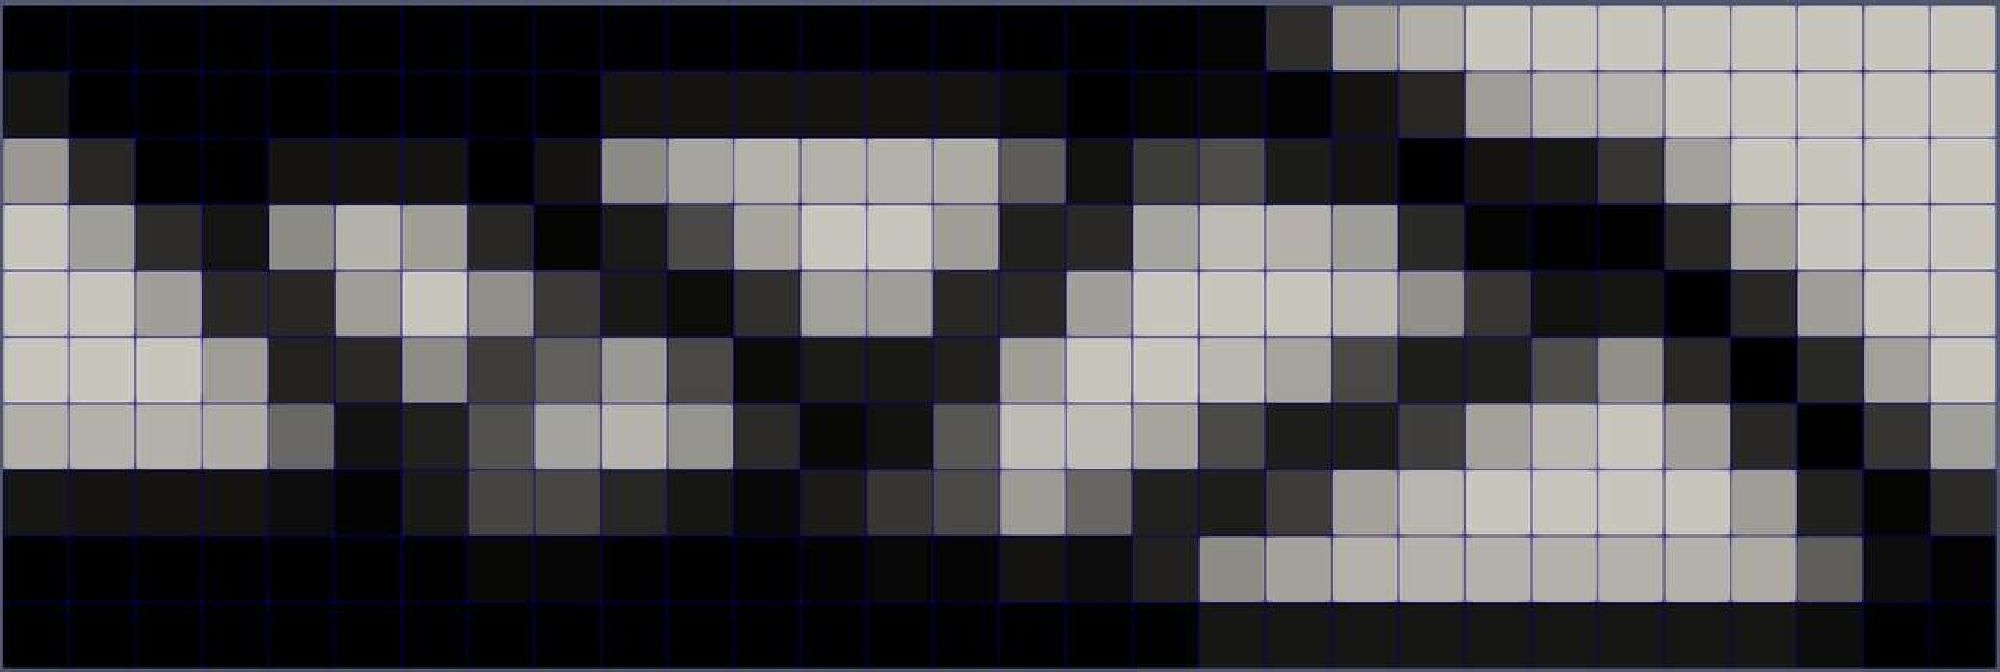
\includegraphics[width=0.92\linewidth,
						height=0.22\paperheight, keepaspectratio]{topo_ana_k4}
					\end{center}
					{\fontsize{7}{10.5}\selectfont\sffamily\centering\par
						$\rho_{\mathrm{dof}} = 300,u_{\mathrm{dof}} = 9922\;\uparrow$ \\[3pt]
						主骨架基本一致，拓扑细节无明显改善}
				\end{tcolorbox}
			\end{column}
			
			% ─── 第三栏：仅提高设计分辨率 ─────────────────────
			\begin{column}{0.32\linewidth}
				\begin{tcolorbox}[
					colback=white, colframe=structure.fg!50,
					colbacktitle=structure.fg, coltitle=white,
					fonttitle=\fontsize{7.5}{10}\selectfont\bfseries\sffamily,
					title={\begin{minipage}[c][3.0em][c]{\linewidth}%
							\circnum{03}\enspace 仅提高设计分辨率：$4\times 4$ 子密度%
					\end{minipage}},
					arc=3pt, boxrule=0.5pt,
					toptitle=0.25pt, bottomtitle=0.25pt,
					top=4pt, bottom=4pt, left=5pt, right=5pt,
					valign=top]
					\begin{center}
						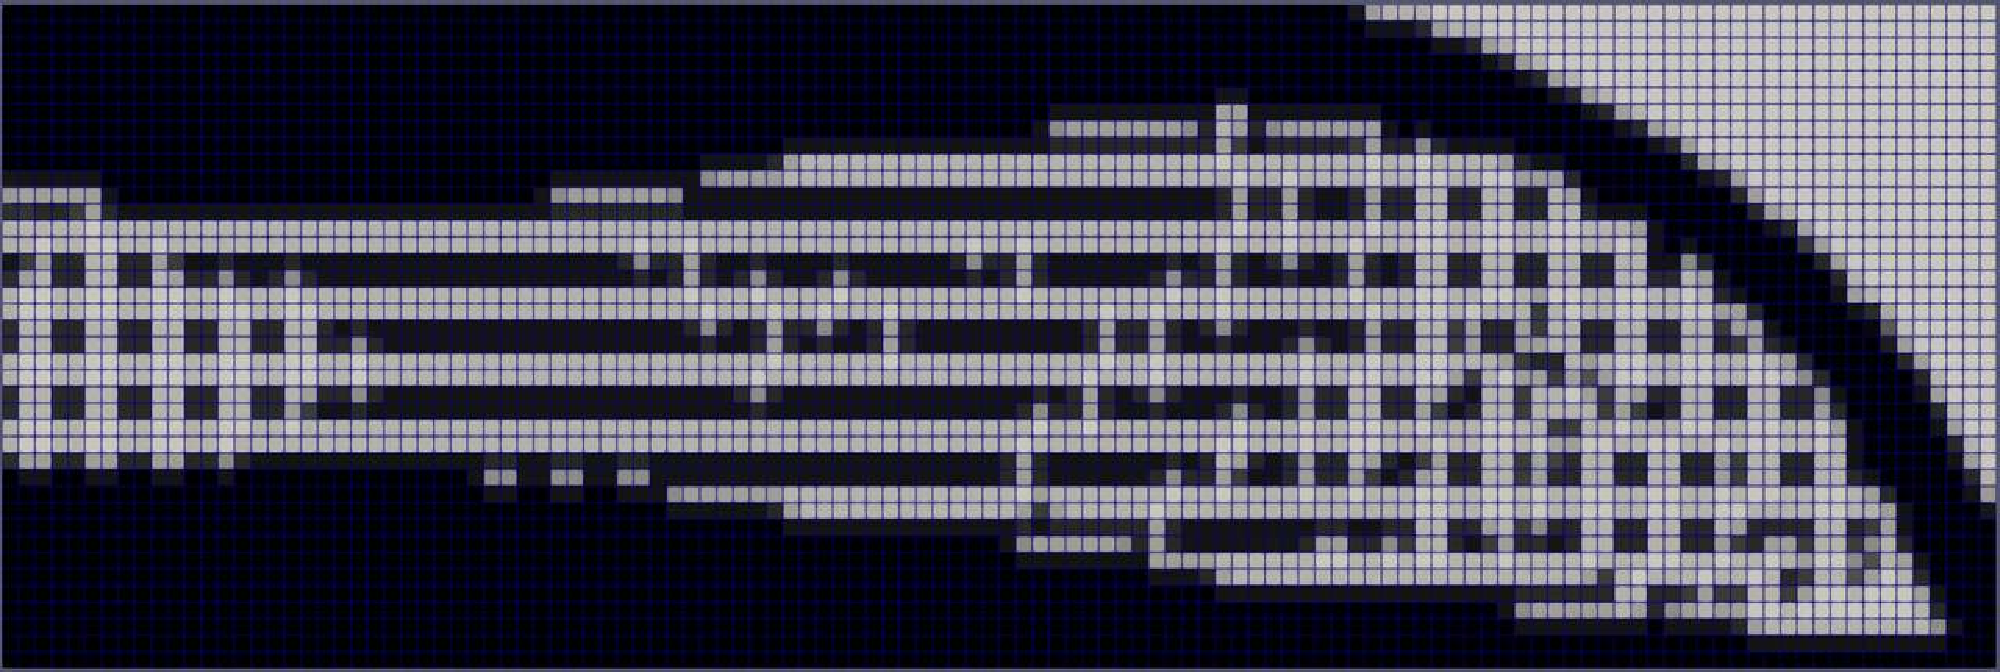
\includegraphics[width=0.92\linewidth,
						height=0.22\paperheight, keepaspectratio]{topo_design_osc}
					\end{center}
					{\fontsize{7}{10.5}\selectfont\sffamily\centering\par
						$u_{\mathrm{dof}} = 2562,\rho_{\mathrm{dof}} = 4800\uparrow$ \\[3pt]
						出现高频震荡与局部伪结构，欠解析显著}
				\end{tcolorbox}
			\end{column}
			
		\end{columns}
		
		% ── 底部总结条 ───────────────────────────────────────────
		\begin{tcolorbox}[
			colback=structure.fg, colframe=structure.fg,
			arc=3pt, boxrule=0pt,
			top=4pt, bottom=4pt, left=8pt, right=8pt]
			\centering
			{\fontsize{8.5}{12}\selectfont\sffamily\color{white}
				设计模型与分析模型刚性绑定 $\Rightarrow$ 单侧提升难以兼顾分析精度与设计分辨率，
				需引入\textbf{多分辨率解耦机制}}
		\end{tcolorbox}
		
	\end{frame}
	
	% ============================================================
	%  04-2  多分辨率空间离散策略
	% ============================================================
	
	\begin{frame}
		\frametitle{多分辨率空间离散策略}
		
		% ── 引导语 ───────────────────────────────────────────────
		\begin{tcolorbox}[
			colback=structure.fg!8, colframe=structure.fg!40,
			arc=2pt, boxrule=0.4pt,
			top=3pt, bottom=3pt, left=8pt, right=8pt]
			\centering
			{\fontsize{8}{11}\selectfont\sffamily
				引入\textbf{“位移网格 — 密度积分网格 — 设计变量网格”}三层离散体系}
		\end{tcolorbox}
		
		% ── 中部：三层网格示意图（单张图） ───────────────────────
		\begin{center}
			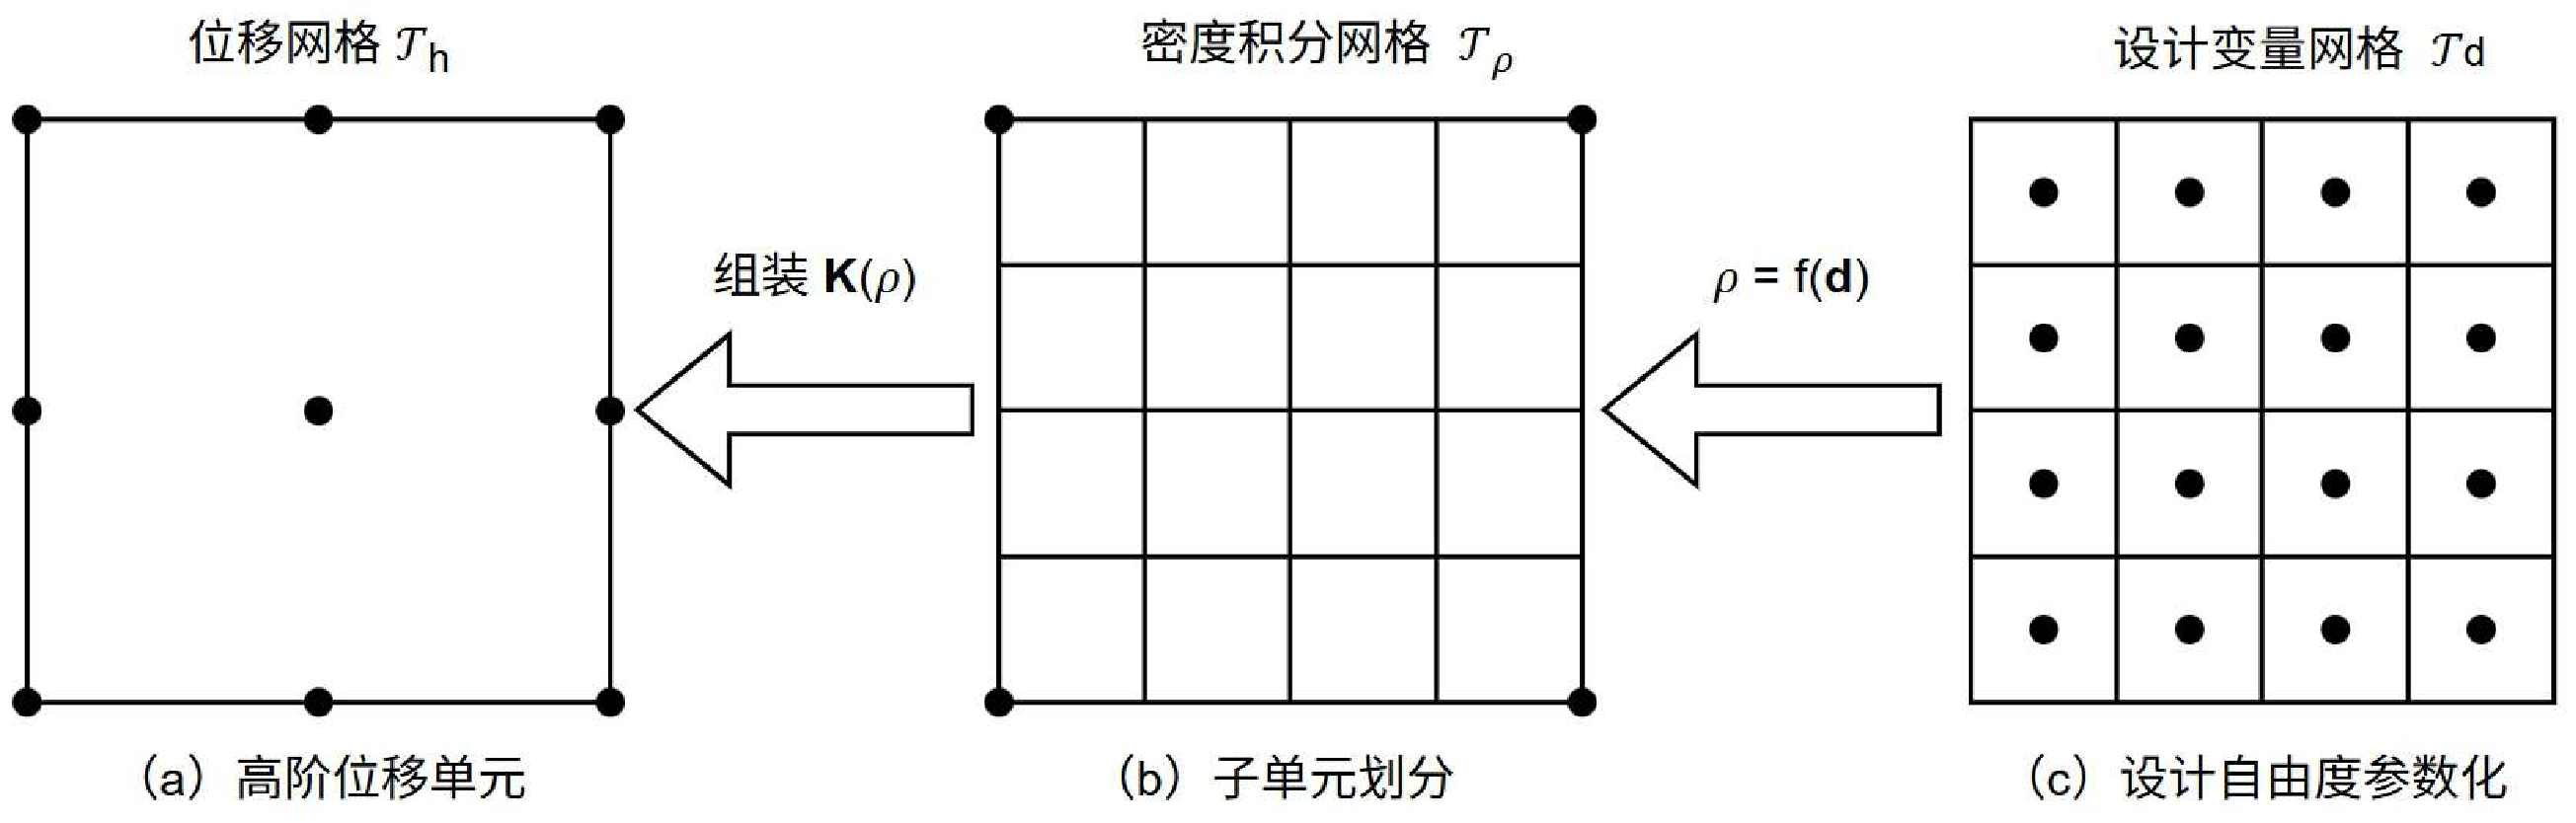
\includegraphics[width=0.88\linewidth, height=0.26\paperheight,
			keepaspectratio]{multires_framework}
		\end{center}
		
		\vspace{-1.5em}
		
		% ── 三栏说明 ─────────────────────────────────────────────
		\begin{columns}[T, totalwidth=\linewidth]
			
			\begin{column}{0.32\linewidth}
				\begin{tcolorbox}[
					colback=white, colframe=structure.fg!50,
					colbacktitle=structure.fg, coltitle=white,
					fonttitle=\fontsize{7.5}{10}\selectfont\bfseries\sffamily,
					title={\begin{minipage}[c][1.4em][c]{\linewidth}\centering
							$\mathcal{T}_h$\enspace 高阶位移网格
					\end{minipage}},
					arc=3pt, boxrule=0.5pt,
					toptitle=0.25pt, bottomtitle=0.25pt,
					top=4pt, bottom=4pt, left=5pt, right=5pt]
					{\fontsize{7}{10.5}\selectfont\sffamily
						采用\textbf{较粗高阶位移单元}，控制分析自由度规模}
				\end{tcolorbox}
			\end{column}
			
			\begin{column}{0.32\linewidth}
				\begin{tcolorbox}[
					colback=white, colframe=structure.fg!50,
					colbacktitle=structure.fg, coltitle=white,
					fonttitle=\fontsize{7.5}{10}\selectfont\bfseries\sffamily,
					title={\begin{minipage}[c][1.4em][c]{\linewidth}\centering
							$\mathcal{T}_\rho$\enspace 密度积分网格
					\end{minipage}},
					arc=3pt, boxrule=0.5pt,
					toptitle=0.25pt, bottomtitle=0.25pt,
					top=4pt, bottom=4pt, left=5pt, right=5pt]
					{\fontsize{7}{10.5}\selectfont\sffamily
						进行\textbf{子单元密度积分}，保证刚度组装一致性}
				\end{tcolorbox}
			\end{column}
			
			\begin{column}{0.32\linewidth}
				\begin{tcolorbox}[
					colback=white, colframe=structure.fg!50,
					colbacktitle=structure.fg, coltitle=white,
					fonttitle=\fontsize{7.5}{10}\selectfont\bfseries\sffamily,
					title={\begin{minipage}[c][1.4em][c]{\linewidth}\centering
							$\mathcal{T}_d$\enspace 设计变量网格
					\end{minipage}},
					arc=3pt, boxrule=0.5pt,
					toptitle=0.25pt, bottomtitle=0.25pt,
					top=4pt, bottom=4pt, left=5pt, right=5pt]
					{\fontsize{7}{10.5}\selectfont\sffamily
						承载\textbf{高分辨率设计变量}，提升拓扑表达能力}
				\end{tcolorbox}
			\end{column}
			
		\end{columns}
		
		\vspace{0.4em}
		
		% ── 底部结论条 ───────────────────────────────────────────
		\begin{tcolorbox}[
			colback=structure.fg, colframe=structure.fg,
			arc=3pt, boxrule=0pt,
			top=4pt, bottom=4pt, left=8pt, right=8pt]
			\centering
			{\fontsize{8.5}{12}\selectfont\sffamily\color{white}
				通过三层网格解耦，在控制计算规模的同时兼顾\textbf{高精度力学分析}与\textbf{高分辨率拓扑表达}}
		\end{tcolorbox}
		
	\end{frame}
		
	% ============================================================
	%  04-3  多分辨率框架：优化列式与子单元积分
	% ============================================================
	
	\begin{frame}[t] 
		\frametitle{多分辨率框架：优化列式与子单元积分}
		
		\only<1>{
			% ── 第一步：优化问题重构 ─────────────────────────────
			\begin{tcolorbox}[
				colback=structure.fg!5, colframe=structure.fg!60,
				colbacktitle=structure.fg, coltitle=white,
				title={\fontsize{9}{11}\selectfont\sffamily\bfseries 1. 多分辨率离散优化列式},
				arc=3pt, boxrule=0.6pt, left=10pt, right=10pt, top=8pt, bottom=8pt,
				toptitle=3pt, bottomtitle=3pt]
				
				{\fontsize{9}{12}\selectfont\sffamily
					通过映射算子 $\boldsymbol{\rho} = f(\boldsymbol{d})$，实现设计空间至物理空间的映射：}
				
				\vspace{0.6em}
				
				{\small
					\begin{equation*}
						\addtolength{\jot}{-2pt} % 压缩公式行间距
						\begin{aligned}
							\min_{\boldsymbol{d}} \quad & c(\boldsymbol{d}) = \boldsymbol{F}^\top \boldsymbol{U}(\boldsymbol{d}) \\
							\text{s.t.} \quad & \boldsymbol{K}(\boldsymbol{\rho}(\boldsymbol{d})) \boldsymbol{U}(\boldsymbol{d}) = \boldsymbol{F} \\
							& \frac{V(\boldsymbol{\rho}(\boldsymbol{d}))}{V_0} \le V_f \\
							& 0 \le d_i \le 1, \quad i=1,\dots,N_d
						\end{aligned}
				\end{equation*}}
				
				\vspace{0.6em}
				
				{\fontsize{9}{12}\selectfont\sffamily
					\textbf{注：} 优化变量在 $\mathcal{T}_d$ 上更新，物理密度在 $\mathcal{T}_\rho$ 上积分，状态方程在 $\mathcal{T}_h$ 上求解。
				}
			\end{tcolorbox}
		}
		
		\only<2>{
			% ── 第二步：数值积分 ──────────────
			\begin{tcolorbox}[
				colback=structure.fg!5, colframe=structure.fg!60,
				colbacktitle=structure.fg, coltitle=white,
				title={\fontsize{9}{11}\selectfont\sffamily\bfseries 2. 基于子单元的高精度数值积分},
				arc=3pt, boxrule=0.6pt, left=10pt, right=10pt, top=8pt, bottom=8pt,
				toptitle=3pt, bottomtitle=3pt]
				
				{\fontsize{9}{12}\selectfont\sffamily
					\textbf{核心挑战：} 粗位移单元内密度场高度非均匀，常规粗单元积分难以准确刻画局部刚度贡献。\\
					\textbf{解决方案：} 引入子单元分段积分策略：}
				
				{\small
					\begin{equation*}
						\addtolength{\jot}{-2pt}
						\begin{aligned}
							\boldsymbol{K}_e 
							&= \int_{\Omega_e} \boldsymbol{B}^\top \boldsymbol{D}(\rho) \boldsymbol{B} \,\mathrm{d}\boldsymbol{x} = \sum_{i=1}^{N_e} \int_{\Omega_{e,i}} \boldsymbol{B}^\top \boldsymbol{D}(\rho_{e,i}) \boldsymbol{B} \,\mathrm{d}\boldsymbol{x} \\ 
							&\approx {\sum_{i=1}^{N_e}} \sum_{g=1}^{N_g} \boldsymbol{B}_{i,g}^\top \boldsymbol{D}(\rho_{e,i}) \boldsymbol{B}_{i,g} w_g {|\det(\boldsymbol{J}_e)| J_i}
						\end{aligned}
					\end{equation*}
				}
				
				{\fontsize{9}{12}\selectfont\sffamily
					\begin{itemize}
						\item \textbf{空间细化：} 以 $N_e$ 个子单元分段求和替代粗单元整体积分，降低欠解析误差；
						\item \textbf{计算优化：} 算子 $\boldsymbol{B}$ 矩阵可预计算缓存，保障组装效率。
				\end{itemize}}
			\end{tcolorbox}
		}
		
	\end{frame}
	
	% ============================================================
	%  04-4  多分辨率框架：灵敏度分析与跨网格传导
	% ============================================================
	
	\begin{frame}[t]
		\frametitle{多分辨率框架：灵敏度分析与跨网格传导}
		
		\only<1>{
			% ── 第一步：物理密度层级的局部灵敏度 ───────────────────────────
			\begin{tcolorbox}[
				colback=structure.fg!5, colframe=structure.fg!60,
				colbacktitle=structure.fg, coltitle=white,
				title={\fontsize{9}{11}\selectfont\sffamily\bfseries 1. 物理密度层级的局部灵敏度},
				arc=3pt, boxrule=0.6pt, left=10pt, right=10pt, top=8pt, bottom=8pt,
				toptitle=3pt, bottomtitle=3pt]
				
				{\fontsize{9}{12}\selectfont\sffamily
					由柔顺度问题的自伴随性，目标函数对位移单元 $\Omega_e$ 内第 $i$ 个子单元物理密度 $\rho_{e,i}$ 的偏导数仅取决于该子单元的刚度贡献：}
				
				\vspace{0.6em}
				
				{\small
					\begin{equation*}
						\addtolength{\jot}{-2pt}
						\begin{aligned}
							\frac{\partial c}{\partial \rho_{e,i}} &= - \boldsymbol{U}_e^\top \frac{\partial \boldsymbol{K}_e}{\partial \rho_{e,i}} \boldsymbol{U}_e \\
							\frac{\partial \boldsymbol{K}_e}{\partial \rho_{e,i}} &= \int_{\Omega_{e,i}} \boldsymbol{B}^\top \frac{\partial \boldsymbol{D}}{\partial \rho}(\rho_{e,i}) \boldsymbol{B} \,\mathrm{d}\boldsymbol{x}
						\end{aligned}
				\end{equation*}}
				
				\vspace{0.4em}
				
				{\fontsize{9}{12}\selectfont\sffamily
					\textbf{物理意义：} 该灵敏度本质上表征了子单元局部的刚度（应变能）积分贡献，它是驱动高分辨率设计变量演化的根本物理依据。}
			\end{tcolorbox}
		}
		
		\only<2>{
			% ── 第二步：跨网格链式法则传导 ───────────────────────────
			\begin{tcolorbox}[
				colback=structure.fg!5, colframe=structure.fg!60,
				colbacktitle=structure.fg, coltitle=white,
				title={\fontsize{9}{11}\selectfont\sffamily\bfseries 2. 跨网格链式法则传导},
				arc=3pt, boxrule=0.6pt, left=10pt, right=10pt, top=8pt, bottom=8pt,
				toptitle=3pt, bottomtitle=3pt]
				
				{\fontsize{9}{12}\selectfont\sffamily
					定义受设计变量 $d_j$ 扰动影响的紧支撑子单元集合 $\mathcal{S}_j := \{(e,i) : \partial \rho_{e,i} / \partial d_j \ne 0\}$。利用链式法则将灵敏度从物理空间传回设计空间：}
				
				\vspace{0.6em}
				
				{\small
					\begin{equation*}
						\frac{\partial c}{\partial d_j} = {\sum_{(e,i) \in \mathcal{S}_j}} \frac{\partial c}{\partial \rho_{e,i}} {\frac{\partial \rho_{e,i}}{\partial d_j}}
				\end{equation*}}
				
				\vspace{0.4em}
				
				{\fontsize{9}{12}\selectfont\sffamily
					\begin{itemize}
						\item \textbf{雅可比项 $\frac{\partial \rho_{e,i}}{\partial d_j}$：} 取决于具体的映射算子（如密度过滤或非线性投影）；
						\item \textbf{数值一致性：} 该列式保证了多分辨率离散体系下目标函数梯度传导的准确性；
						\item \textbf{支撑集 $\mathcal{S}_j$：} 确保了计算的高效性，仅在变量影响域内进行求和累加。
				\end{itemize}}
			\end{tcolorbox}
		}
		
	\end{frame}
	
	% ============================================================
	%  04-5  多分辨率框架中的密度映射机制
	% ============================================================
	
	\begin{frame}
		\frametitle{多分辨率框架中的密度映射机制}
		
		% ─── 顶部引导语 ─────────────────────────────────
		\begin{tcolorbox}[
			colback=structure.fg!5,
			colframe=structure.fg!35,
			boxrule=0.45pt,
			arc=3pt,
			left=7pt, right=7pt, top=3pt, bottom=3pt]
			{\fontsize{8.0}{10.2}\selectfont\sffamily
				映射算子 $\rho=f(\boldsymbol d)$ 将设计变量传递到密度积分网格，
				并影响刚度矩阵组装、灵敏度传导与最终拓扑构型。
			}
		\end{tcolorbox}
		
		% ─── 中部统一流程 ─────────────────
		\begin{center}
			\resizebox{0.90\linewidth}{!}{$
				\boxed{d \in \mathcal{T}_d}
				\quad
				\xrightarrow{\ \rho=f(d)\ }
				\quad
				\boxed{\rho_{e,i}\in \mathcal{T}_{\rho}}
				\quad
				\xrightarrow{\ \text{子单元积分 / 链式传导}\ }
				\quad
				\boxed{K(\rho),\ \dfrac{\partial c}{\partial d_j}}
				$}
		\end{center}
		
		% ─── Overlay 1：灵敏度过滤 / 恒等映射 ───────────────
		\only<1>{
			\begin{center}
				\begin{tcolorbox}[
					width=0.965\paperwidth,
					colback=white,
					colframe=structure.fg!55,
					colbacktitle=structure.fg,
					coltitle=white,
					fonttitle=\fontsize{8.4}{10.2}\selectfont\bfseries\sffamily,
					title={01\quad 灵敏度过滤：恒等映射},
					arc=3pt,
					boxrule=0.5pt,
					toptitle=0.3pt,
					bottomtitle=0.3pt,
					top=8pt, bottom=8pt, left=11pt, right=11pt,
					height=0.34\paperheight]
					
					{\fontsize{8.0}{11.2}\selectfont\sffamily
						\begin{columns}[T, totalwidth=\linewidth]
							
							% ─── 左侧：核心公式 ─────────────────────
							\begin{column}{0.38\linewidth}
								\vspace{0.70em}
								
								\[
								\scalebox{1.22}{$\displaystyle \rho_{e,i}=d_{j}$}
								\]
								
								\vspace{0.9em}
								
								\begin{center}
									{\fontsize{8.1}{10.8}\selectfont\sffamily
										\textbf{设计变量与物理密度直接对应}
									}
								\end{center}
							\end{column}
							
							% ─── 右侧：机制解释 ─────────────────────
							\begin{column}{0.58\linewidth}
								\setbeamertemplate{itemize item}{\raisebox{1pt}{\tiny$\bullet$}}
								\setlength{\leftmargini}{1.0em}
								\begin{itemize}
									\setlength{\itemsep}{5pt}
									\setlength{\topsep}{1pt}
									\setlength{\parsep}{0pt}
									\setlength{\parskip}{0pt}
									\item 物理密度场不经过额外平滑或投影处理；
									\item 过滤只作用于灵敏度更新，不改变 $\rho=f(d)$ 的恒等关系；
									\item 机制最直接，可作为密度过滤与非线性投影的基准对照。
								\end{itemize}
							\end{column}
							
						\end{columns}
					}
				\end{tcolorbox}
			\end{center}
		}
		
		% ═════════════════════════════════════════════════════
		%  Overlay 2：密度过滤 / 线性映射
		% ═════════════════════════════════════════════════════
		\only<2>{
			\begin{center}
				\begin{tcolorbox}[
					width=0.965\paperwidth,
					colback=white,
					colframe=structure.fg!55,
					colbacktitle=structure.fg,
					coltitle=white,
					fonttitle=\fontsize{8.4}{10.2}\selectfont\bfseries\sffamily,
					title={02\quad 密度过滤：线性映射},
					arc=3pt,
					boxrule=0.5pt,
					toptitle=0.3pt,
					bottomtitle=0.3pt,
					top=8pt, bottom=8pt, left=11pt, right=11pt,
					height=0.34\paperheight]
					
					{\fontsize{8.0}{11.2}\selectfont\sffamily
						\begin{columns}[T, totalwidth=\linewidth]
							
							% ─── 左侧：核心公式 ─────────────────────
							\begin{column}{0.47\linewidth}
								\vspace{0.15em}
								
								\[
								\scalebox{1.02}{$\displaystyle
									\rho_{e,i}
									=
									\frac{
										\sum\limits_{j\in\mathcal{N}_{e,i}}
										H_{(e,i)j} v_j d_j
									}{
										\sum\limits_{j\in\mathcal{N}_{e,i}}
										H_{(e,i)j} v_j
									}
									$}
								\]
								
								\vspace{0.55em}
								
								\begin{center}
									{\fontsize{8.0}{10.5}\selectfont\sffamily
										\textbf{归一化加权平均得到物理密度}
									}
								\end{center}
							\end{column}
							
							% ─── 右侧：机制解释 ─────────────────────
							\begin{column}{0.49\linewidth}
								\setbeamertemplate{itemize item}{\raisebox{1pt}{\tiny$\bullet$}}
								\setlength{\leftmargini}{1.0em}
								\begin{itemize}
									\setlength{\itemsep}{5pt}
									\setlength{\topsep}{1pt}
									\setlength{\parsep}{0pt}
									\setlength{\parskip}{0pt}
									\item $\mathcal{N}_{e,i}$：子单元 $(e,i)$ 相关的设计变量邻域；
									\item $H_{(e,i)j}$：由子单元中心坐标与设计变量位置确定的过滤权重；
									\item 对邻域内 $d_j$ 归一化加权平均，实现尺度控制与密度平滑。
								\end{itemize}
							\end{column}
							
						\end{columns}
					}
				\end{tcolorbox}
			\end{center}
		}
		
		% ═════════════════════════════════════════════════════
		%  Overlay 3：非线性投影 / 复合映射
		% ═════════════════════════════════════════════════════
		\only<3>{
			\begin{center}
				\begin{tcolorbox}[
					width=0.965\paperwidth,
					colback=white,
					colframe=structure.fg!55,
					colbacktitle=structure.fg,
					coltitle=white,
					fonttitle=\fontsize{8.4}{10.2}\selectfont\bfseries\sffamily,
					title={03\quad 非线性投影：复合映射},
					arc=3pt,
					boxrule=0.5pt,
					toptitle=0.3pt,
					bottomtitle=0.3pt,
					top=8pt, bottom=8pt, left=11pt, right=11pt,
					height=0.34\paperheight]
					
					{\fontsize{8.0}{11.2}\selectfont\sffamily
						\begin{columns}[T, totalwidth=\linewidth]
							
							% ─── 左侧：核心公式 ─────────────────────
							\begin{column}{0.48\linewidth}
								\vspace{-0.10em}
								
								\[
								\scalebox{1.05}{$\displaystyle
									d_j
									\longrightarrow
									\widetilde{\rho}_{e,i}
									\longrightarrow
									\rho_{e,i}
									$}
								\]
								
								\vspace{-1.0em}
								
								\[
								\scalebox{0.88}{$\displaystyle
									\rho_{e,i}
									=
									\frac{
										\tanh(\beta\eta)
										+
										\tanh\!\bigl(\beta(\widetilde{\rho}_{e,i}-\eta)\bigr)
									}{
										\tanh(\beta\eta)
										+
										\tanh\!\bigl(\beta(1-\eta)\bigr)
									}
									$}
								\]
								
								%								\vspace{-0.10em}
								
								\begin{center}
									{\fontsize{8.0}{10.5}\selectfont\sffamily
										\textbf{线性过滤后叠加双曲正切投影}
									}
								\end{center}
							\end{column}
							
							% ─── 右侧：机制解释 ─────────────────────
							\begin{column}{0.48\linewidth}
								\setbeamertemplate{itemize item}{\raisebox{1pt}{\tiny$\bullet$}}
								\setlength{\leftmargini}{1.0em}
								\begin{itemize}
									\setlength{\itemsep}{5pt}
									\setlength{\topsep}{1pt}
									\setlength{\parsep}{0pt}
									\setlength{\parskip}{0pt}
									\item 先由密度过滤得到中间密度 $\widetilde{\rho}_{e,i}$，
									再经投影生成最终物理密度 $\rho_{e,i}$；
									\item $\eta$ 为投影阈值，$\beta$ 控制投影陡峭程度；
									\item 逐步增大 $\beta$，增强 $0$--$1$ 二值化与边界清晰度。
								\end{itemize}
							\end{column}
							
						\end{columns}
					}
				\end{tcolorbox}
			\end{center}
		}
		
		% ─── 底部标准结论框 ───────────────────────────────
		\begin{tcolorbox}[
			colback=structure.fg,
			colframe=structure.fg,
			coltext=white,
			boxrule=0.45pt,
			arc=3pt,
			left=7pt, right=7pt, top=3pt, bottom=3pt]
			\centering
			{\fontsize{7.8}{9.8}\selectfont\sffamily
				不同映射机制改变 $\rho=f(d)$ 的正则化方式，从而影响后续构型清晰度与算法鲁棒性。
			}
		\end{tcolorbox}
		
	\end{frame}
	
	% ============================================================
	%  04-6  多分辨率数值验证：基准算例与参考构型
	% ============================================================
	
	\begin{frame}
		\frametitle{多分辨率数值验证：基准算例与参考构型}
		
		% ─── 顶部引导语 ─────────────────────────────────
		\begin{tcolorbox}[
			colback=structure.fg!5,
			colframe=structure.fg!35,
			boxrule=0.45pt,
			arc=3pt,
			left=7pt, right=7pt, top=3pt, bottom=3pt]
			{\fontsize{8.0}{10.2}\selectfont\sffamily
				以二维 MBB 梁为统一基准算例，对照 Michell 型扇形桁架，检验多分辨率框架的拓扑细节表达能力。
			}
		\end{tcolorbox}
		
		\vspace{-0.5em}
		
		% ═════════════════════════════════════════════════════
		%  主体双栏：二维 MBB 梁 / Michell 型参考构型
		% ═════════════════════════════════════════════════════
		\begin{columns}[T, totalwidth=\linewidth]
			
			% ─── 左栏：二维 MBB 梁基准算例 ─────────────────
			\begin{column}{0.485\linewidth}
				\begin{tcolorbox}[
					colback=white,
					colframe=structure.fg!55,
					colbacktitle=structure.fg,
					coltitle=white,
					fonttitle=\fontsize{8.2}{10}\selectfont\bfseries\sffamily,
					title={01\quad 二维 MBB 梁基准算例},
					arc=3pt,
					boxrule=0.5pt,
					toptitle=0.3pt,
					bottomtitle=0.3pt,
					top=5pt, bottom=5pt, left=7pt, right=7pt,
					height=0.50\paperheight]
					
					{\fontsize{7.25}{10.2}\selectfont\sffamily
						\begin{center}
							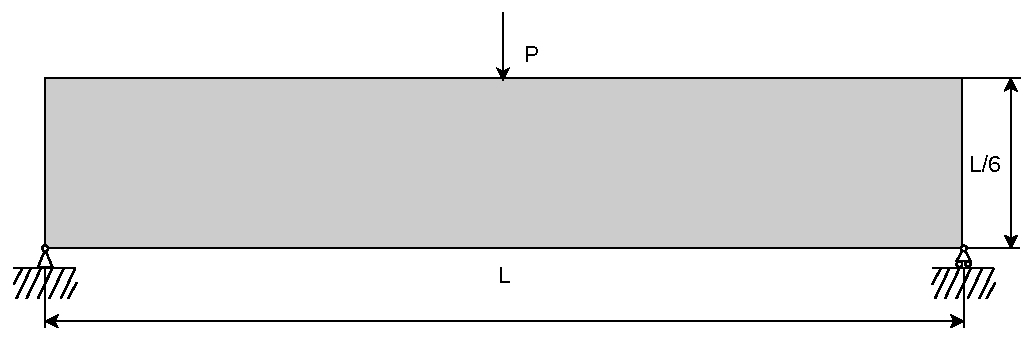
\includegraphics[
							width=0.96\linewidth,
							height=0.24\paperheight,
							keepaspectratio
							]{mbb2d_setup}
						\end{center}
						
						\vspace{0.10em}
						
						\setbeamertemplate{itemize item}{\raisebox{1pt}{\tiny$\bullet$}}
						\setlength{\leftmargini}{0.90em}
						\begin{itemize}
							\setlength{\itemsep}{2pt}
							\setlength{\topsep}{1pt}
							\setlength{\parsep}{0pt}
							\setlength{\parskip}{0pt}
							\item 几何尺寸为 $L\times L/6$；取 $L=60\,\mathrm{mm}$，$E=1\,\mathrm{MPa}$，$\nu=0.3$，$V_f=0.6$。
							\item 左下角铰支约束，右下角滑移约束，上边中点施加竖向载荷 $P=2\,\mathrm{N}$。
						\end{itemize}
					}
				\end{tcolorbox}
			\end{column}
			
			% ─── 右栏：Michell 型扇形桁架参考构型 ───────────
			\begin{column}{0.485\linewidth}
				\begin{tcolorbox}[
					colback=white,
					colframe=structure.fg!55,
					colbacktitle=structure.fg,
					coltitle=white,
					fonttitle=\fontsize{8.2}{10}\selectfont\bfseries\sffamily,
					title={02\quad Michell 型扇形桁架参考构型},
					arc=3pt,
					boxrule=0.5pt,
					toptitle=0.3pt,
					bottomtitle=0.3pt,
					top=5pt, bottom=5pt, left=7pt, right=7pt,
					height=0.50\paperheight]
					
					{\fontsize{7.25}{10.2}\selectfont\sffamily
						\begin{center}
							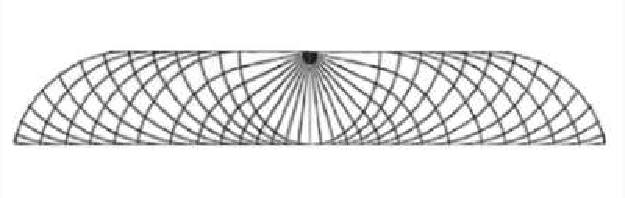
\includegraphics[
							width=0.96\linewidth,
							height=0.24\paperheight,
							keepaspectratio
							]{mbb2d_michell}
						\end{center}
						
						\vspace{0.10em}
						
						\setbeamertemplate{itemize item}{\raisebox{1pt}{\tiny$\bullet$}}
						\setlength{\leftmargini}{0.90em}
						\begin{itemize}
							\setlength{\itemsep}{2pt}
							\setlength{\topsep}{1pt}
							\setlength{\parsep}{0pt}
							\setlength{\parskip}{0pt}
							\item 体现集中载荷作用下的典型主传力路径与扇形分支结构。
							\item 为评价优化构型的拓扑细节表达与力学合理性提供参考。
						\end{itemize}
					}
				\end{tcolorbox}
			\end{column}
			
		\end{columns}
		
	\end{frame}
	
	% ============================================================
	%  04-7  多分辨率框架下的拓扑表达优势
	% ============================================================
	
	\begin{frame}
		\frametitle{多分辨率框架下的拓扑表达优势}
		
		% ── 引导语 ───────────────────────────────────────────────
		\begin{tcolorbox}[
			colback=structure.fg!8, colframe=structure.fg!40,
			arc=2pt, boxrule=0.4pt,
			top=3pt, bottom=3pt, left=8pt, right=8pt]
			\centering
			{\fontsize{8}{11}\selectfont\sffamily
				以二维 MBB 梁为例，在经典密度过滤（线性映射）下展示多分辨率框架的拓扑表达优势}
		\end{tcolorbox}
		
		% ── 主体：2×2 网格（顶部标识 + 图 + 底部数据） ────────────
		\begin{center}
			\renewcommand{\arraystretch}{1.3}
			\begin{tabular}{@{}c@{\hspace{1.5em}}c@{}}
				
				% ─── (a) STOP k=1 ─────────────────────────────
				\begin{minipage}[t]{0.46\linewidth}
					\centering
					{\fontsize{8}{11}\selectfont\sffamily
						(a)\enspace STOP:\enspace $k=1,r_{\min}=1.2$\par}
					\vspace{2pt}
					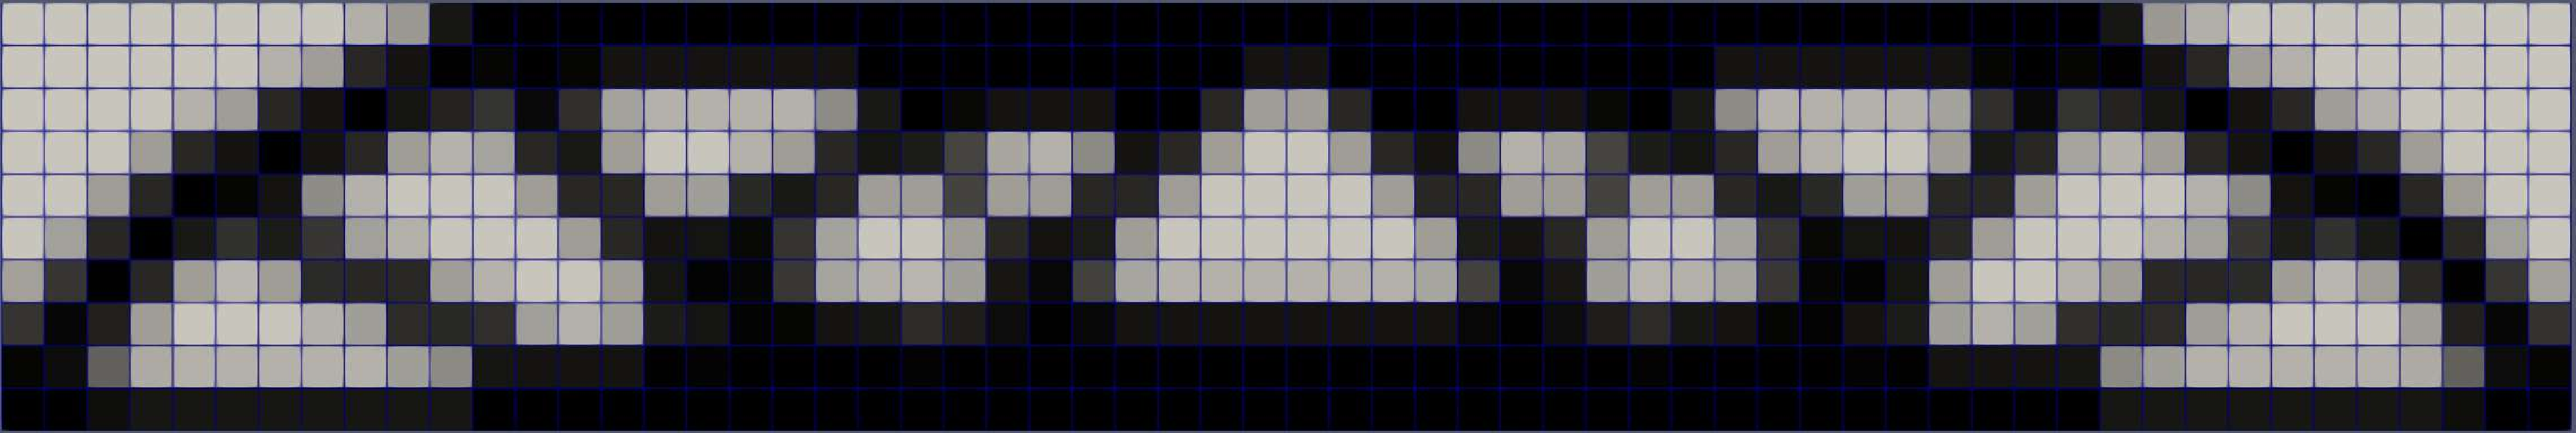
\includegraphics[width=\linewidth,
					height=0.19\paperheight, keepaspectratio]{mbb_stop_k1}\\[2pt]
					{\fontsize{7.5}{10}\selectfont\sffamily
						$\rho_{\mathrm{dof}}=600,\;u_{\mathrm{dof}}=1342$}
				\end{minipage}
				
				&
				
				% ─── (b) MTOP k=1 ─────────────────────────────
				\begin{minipage}[t]{0.46\linewidth}
					\centering
					{\fontsize{8}{11}\selectfont\sffamily
						(b)\enspace MTOP:\enspace $k=1,r_{\min}=1.0$\par}
					\vspace{2pt}
					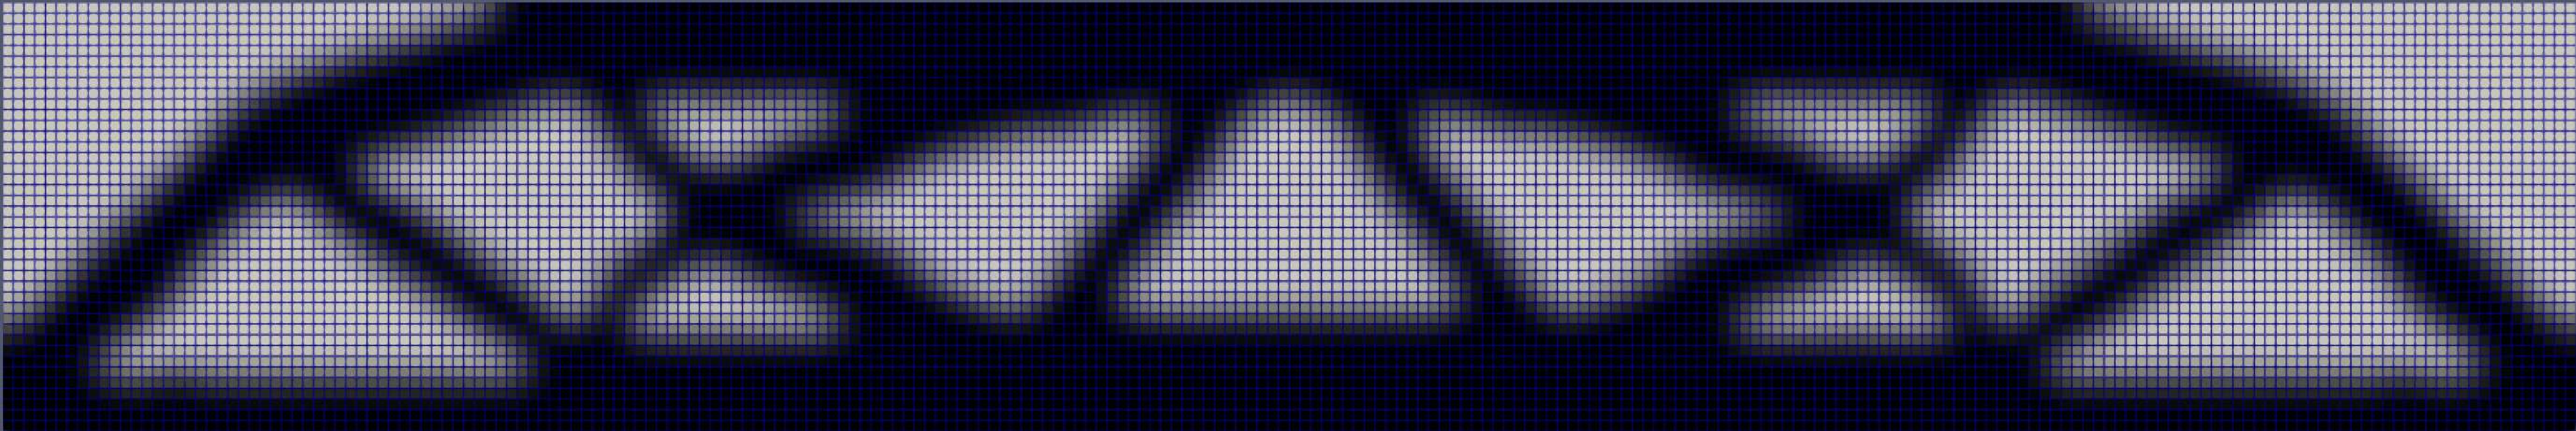
\includegraphics[width=\linewidth,
					height=0.19\paperheight, keepaspectratio]{mbb_mtop_k1}\\[2pt]
					{\fontsize{7.5}{10}\selectfont\sffamily
						$\rho_{\mathrm{dof}}=9600,\;u_{\mathrm{dof}}=1342$}
				\end{minipage}
				
				\\
				
				% ─── (c) MTOP k=2 ─────────────────────────────
				\begin{minipage}[t]{0.46\linewidth}
					\centering
					{\fontsize{8}{11}\selectfont\sffamily
						(c)\enspace MTOP:\enspace $k=2,r_{\min}=0.75$\par}
					\vspace{2pt}
					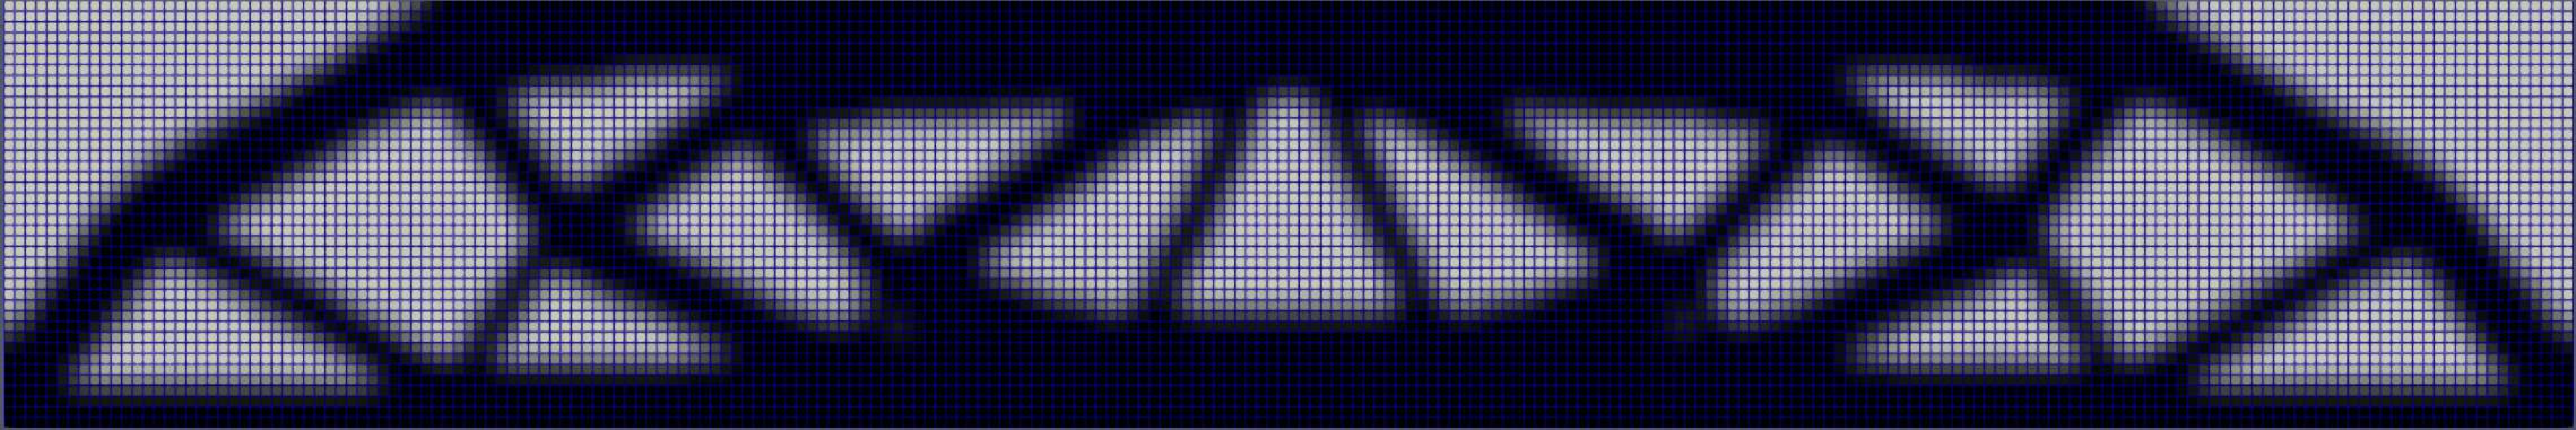
\includegraphics[width=\linewidth,
					height=0.19\paperheight, keepaspectratio]{mbb_mtop_k2}\\[2pt]
					{\fontsize{7.5}{10}\selectfont\sffamily
						$\rho_{\mathrm{dof}}=9600,\;u_{\mathrm{dof}}=5082$}
				\end{minipage}
				
				&
				
				% ─── (d) MTOP k=4 ─────────────────────────────
				\begin{minipage}[t]{0.46\linewidth}
					\centering
					{\fontsize{8}{11}\selectfont\sffamily
						(d)\enspace MTOP:\enspace $k=4,r_{\min}=0.5$\par}
					\vspace{2pt}
					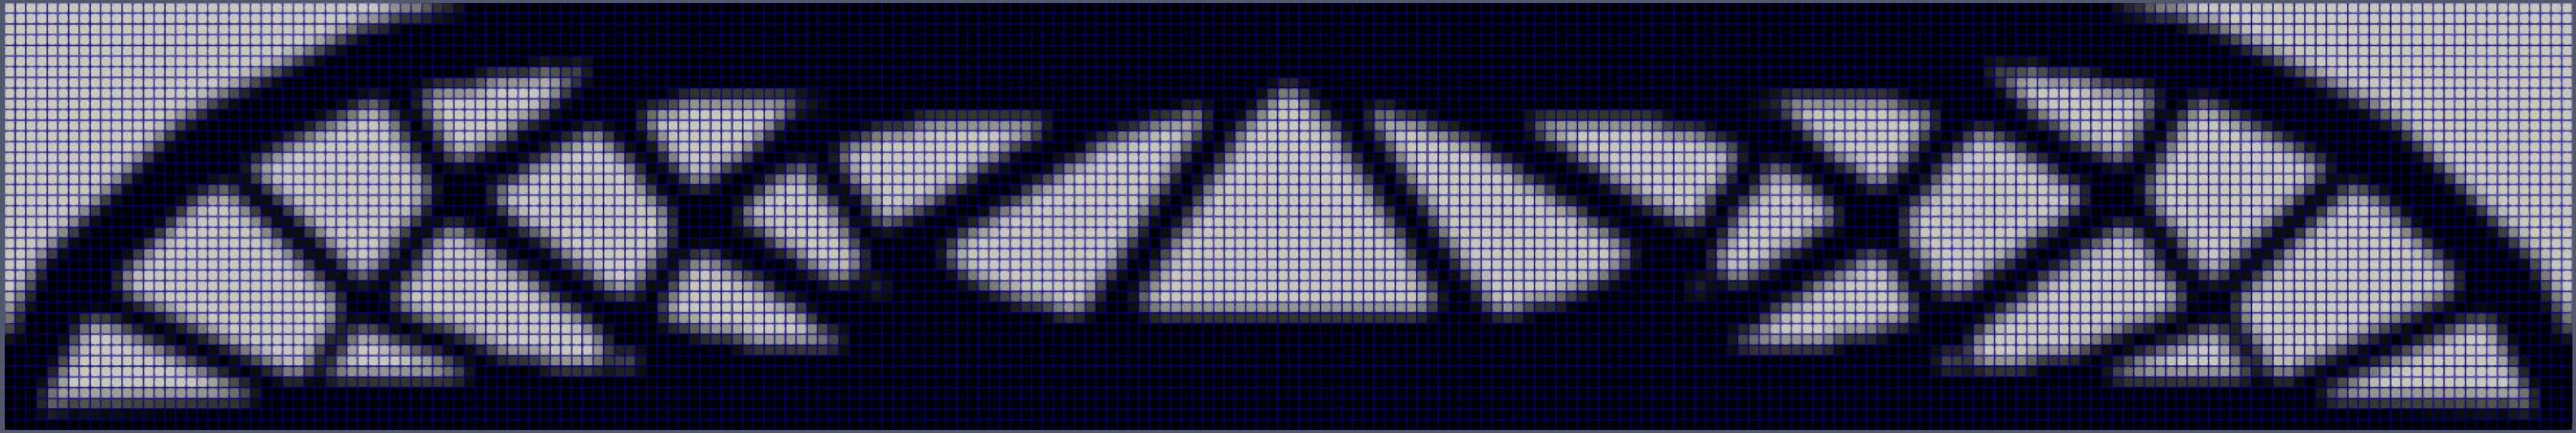
\includegraphics[width=\linewidth,
					height=0.19\paperheight, keepaspectratio]{mbb_mtop_k4}\\[2pt]
					{\fontsize{7.5}{10}\selectfont\sffamily
						$\rho_{\mathrm{dof}}=9600,\;u_{\mathrm{dof}}=19762$}
				\end{minipage}
				
			\end{tabular}
		\end{center}
		
		% ── 底部结论条 ───────────────────────────────────────────
		\begin{tcolorbox}[
			colback=structure.fg, colframe=structure.fg,
			arc=3pt, boxrule=0pt,
			top=4pt, bottom=4pt, left=8pt, right=8pt]
			\centering
			{\fontsize{8.5}{12}\selectfont\sffamily\color{white}
				多分辨率解耦释放高阶有限元分析优势，获得更清晰、细节更丰富的拓扑构型}
		\end{tcolorbox}
		
	\end{frame}
	
	% ============================================================
	%  04-8  密度映射机制与构型鲁棒性
	% ============================================================
	
	\begin{frame}
		\frametitle{密度映射机制与构型鲁棒性}
		
		% ── 引导语 ───────────────────────────────────────────────
		\begin{tcolorbox}[
			colback=structure.fg!8, colframe=structure.fg!40,
			arc=2pt, boxrule=0.4pt,
			top=3pt, bottom=3pt, left=8pt, right=8pt]
			\centering
			{\fontsize{8}{11}\selectfont\sffamily
				在三层多分辨率框架下，进一步比较不同密度映射机制对拓扑构型与算法稳定性的影响}
		\end{tcolorbox}
		
		% ── 左右两栏对照 ──────────────────────────────────────────
		\begin{columns}[T, totalwidth=\linewidth]
			
			% ─── 左栏：灵敏度过滤（恒等映射）─────────────────
			\begin{column}{0.485\linewidth}
				\centering
				% 栏目标题 
				{\fontsize{9}{10}\selectfont\sffamily\bfseries\color{structure.fg}
					灵敏度过滤：恒等映射\par}
				
				\vspace{2pt}
				
				% 子图 1：k=1
				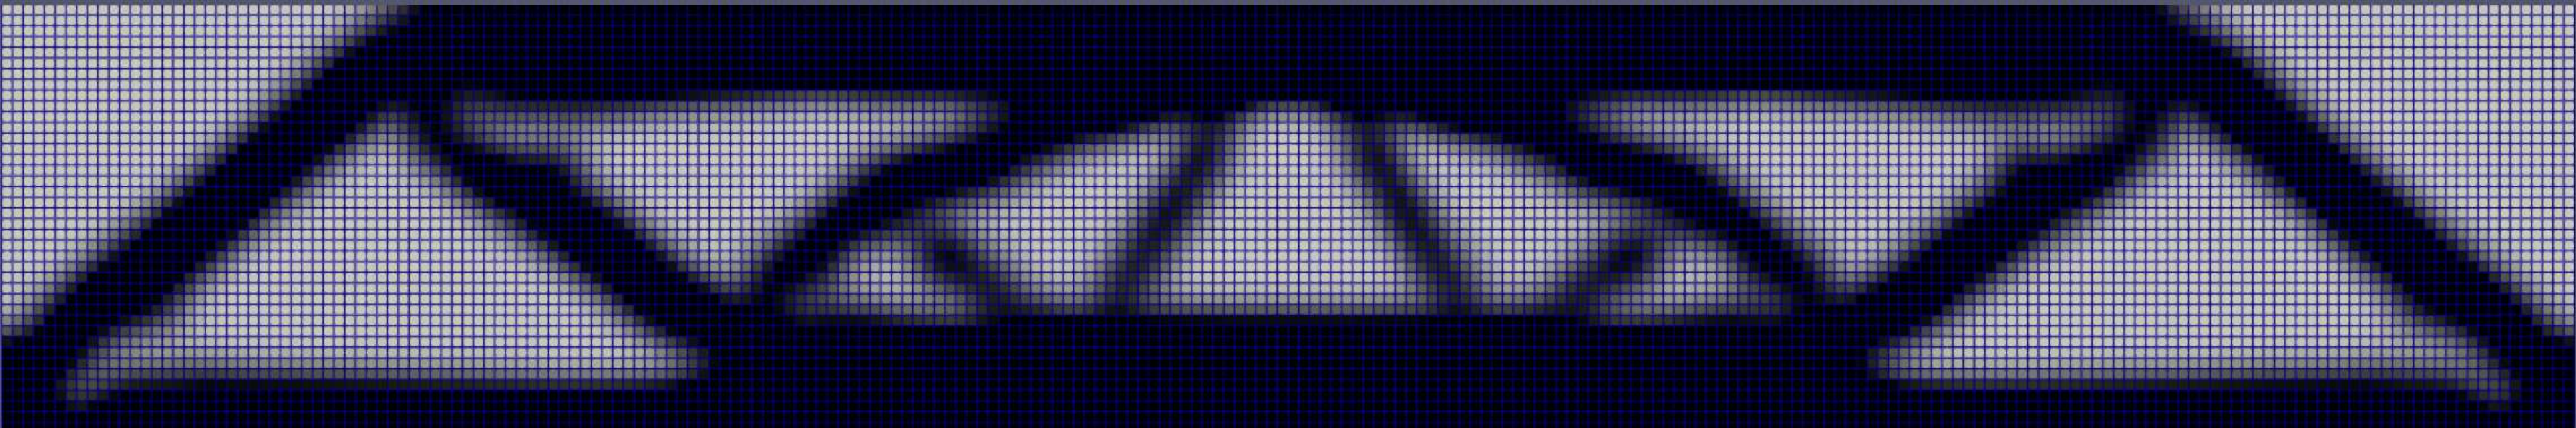
\includegraphics[width=0.92\linewidth, height=0.18\paperheight,
				keepaspectratio]{filter_identity_k1}\\[1pt]
				{\fontsize{7.5}{10}\selectfont\sffamily (a)\enspace $k=1,r_{\min}=1.0$}
				
				\vspace{4pt}
				
				% 子图 2：k=4
				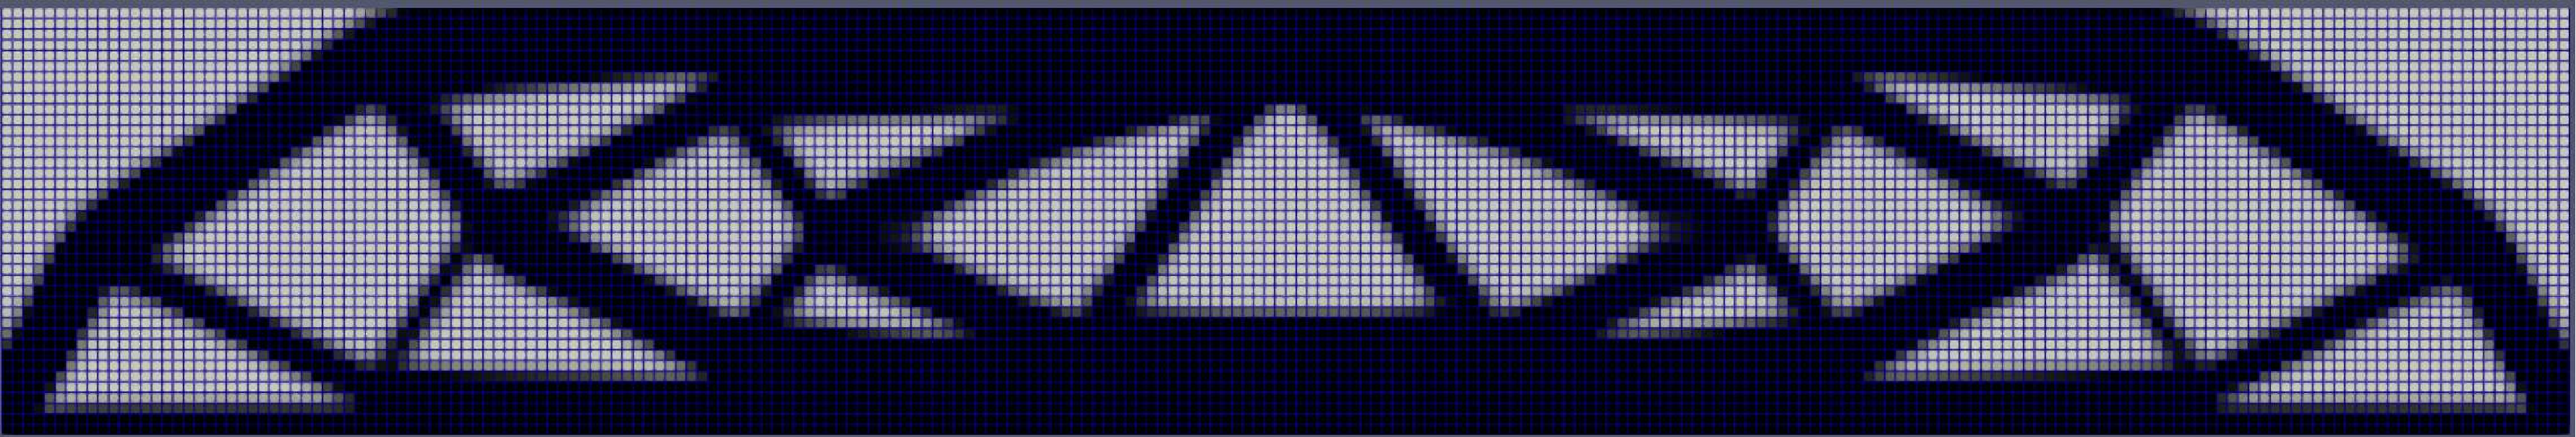
\includegraphics[width=0.92\linewidth, height=0.18\paperheight,
				keepaspectratio]{filter_identity_k4}\\[1pt]
				{\fontsize{7.5}{10}\selectfont\sffamily (b)\enspace $k=4,r_{\min}=0.5$}
				
				\vspace{6pt}
				% 说明
				{\fontsize{7.5}{11}\selectfont\sffamily
					设计变量与物理密度直接对应，构型演化较稳定，但边界灰度过渡较明显}
			\end{column}
			
			% ─── 右栏：非线性投影（复合映射）─────────────────
			\begin{column}{0.485\linewidth}
				\centering
				% 栏目标题 
				{\fontsize{9}{10}\selectfont\sffamily\bfseries\color{structure.fg}
					非线性投影：复合映射\par}
				
				\vspace{2pt}
				
				% 子图 1：k=1
				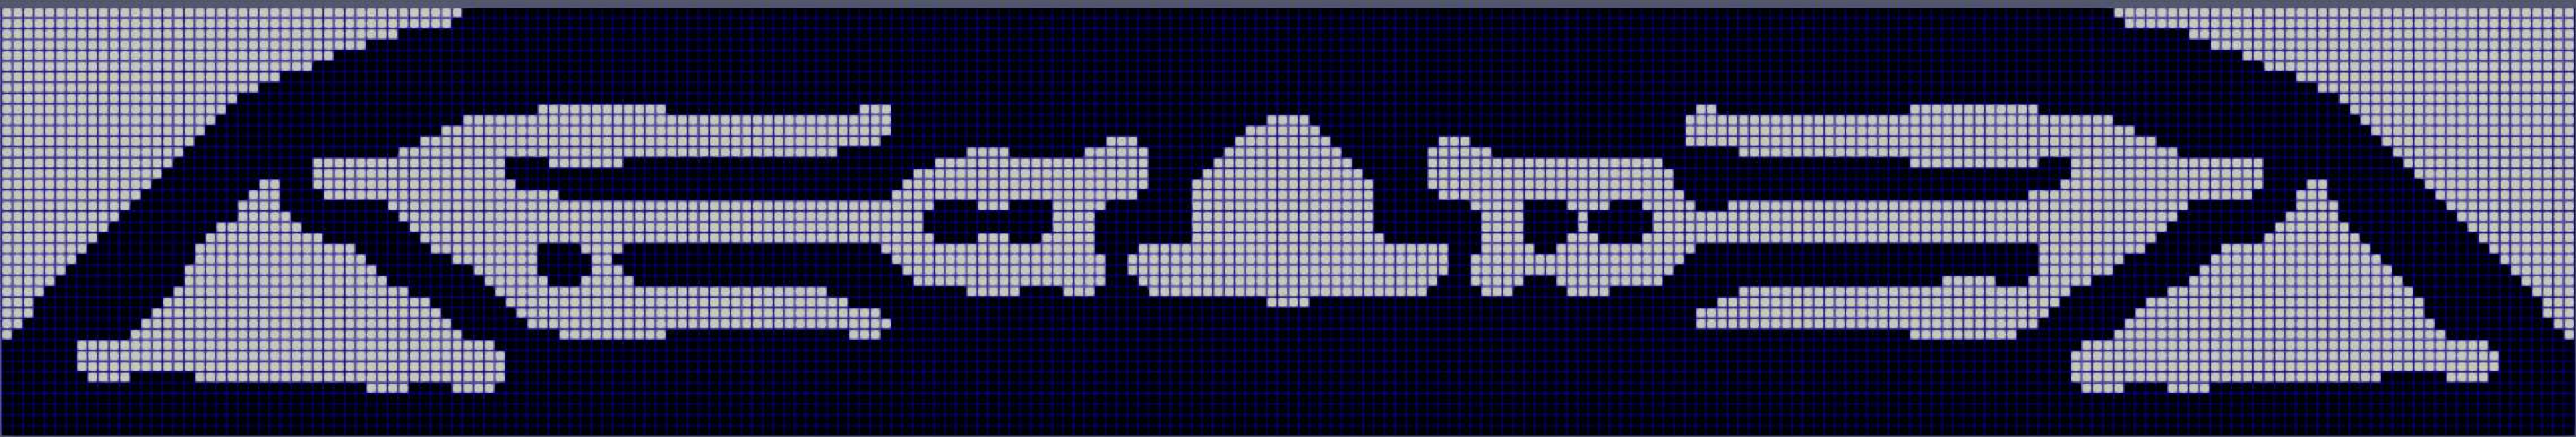
\includegraphics[width=0.92\linewidth, height=0.18\paperheight,
				keepaspectratio]{projection_composite_k1}\\[1pt]
				{\fontsize{7.5}{10}\selectfont\sffamily (c)\enspace $k=1,r_{\min}=1.0$}
				
				\vspace{4pt}
				
				% 子图 2：k=4
				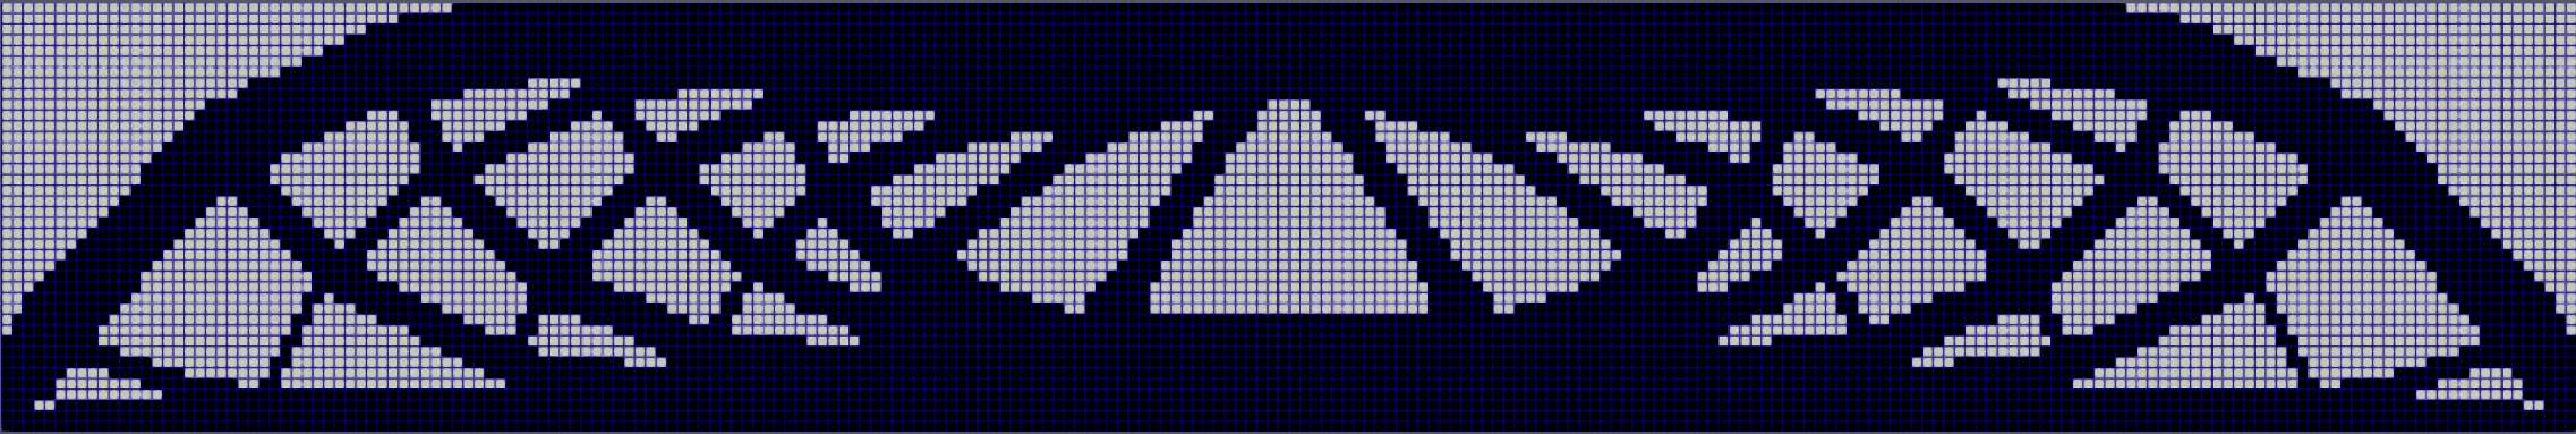
\includegraphics[width=0.92\linewidth, height=0.18\paperheight,
				keepaspectratio]{projection_composite_k4}\\[1pt]
				{\fontsize{7.5}{10}\selectfont\sffamily (d)\enspace $k=4,r_{\min}=0.5$}
				
				\vspace{6pt}
				% 说明
				{\fontsize{7.5}{11}\selectfont\sffamily
					投影增强 0–1 二值化特征，高阶分析下边界更清晰、细节更丰富}
			\end{column}
			
		\end{columns}
		
		% ── 底部结论条 ───────────────────────────────────────────
		\begin{tcolorbox}[
			colback=structure.fg, colframe=structure.fg,
			arc=3pt, boxrule=0pt,
			top=4pt, bottom=4pt, left=8pt, right=8pt]
			\centering
			{\fontsize{8.5}{12}\selectfont\sffamily\color{white}
				将过滤、投影与高阶分析协同耦合，提升了多分辨率拓扑优化的构型质量与算法鲁棒性}
		\end{tcolorbox}
		
	\end{frame}
	
	% ============================================================
	%  04-9  多分辨率应力约束模型
	% ============================================================
	
	\begin{frame}
		\frametitle{多分辨率应力约束模型}
		
		% ─── 顶部引导语 ─────────────────────────────────
		\begin{tcolorbox}[
			colback=structure.fg!5,
			colframe=structure.fg!35,
			boxrule=0.45pt,
			arc=3pt,
			left=7pt, right=7pt, top=3pt, bottom=3pt]
			{\fontsize{8.0}{10.2}\selectfont\sffamily
				在多分辨率框架下，将局部应力约束下沉到密度积分子单元层级，
				从而把高分辨率拓扑表达扩展到局部强度约束设计。
			}
		\end{tcolorbox}
		
		% ═════════════════════════════════════════════════════
		%  Overlay 1：应力约束优化模型
		% ═════════════════════════════════════════════════════
		\only<1>{
			\begin{center}
				\begin{tcolorbox}[
					width=0.965\paperwidth,
					colback=white,
					colframe=structure.fg!55,
					colbacktitle=structure.fg,
					coltitle=white,
					fonttitle=\fontsize{8.4}{10.2}\selectfont\bfseries\sffamily,
					title={01\quad 应力约束优化模型},
					arc=3pt,
					boxrule=0.5pt,
					toptitle=0.3pt,
					bottomtitle=0.3pt,
					top=8pt, bottom=7pt, left=12pt, right=12pt,
					height=0.50\paperheight]
					
					{\fontsize{8.0}{11.2}\selectfont\sffamily
						
						\vspace{-0.25em}
						
						\[
						\begin{aligned}
							\min_{\boldsymbol d}\quad
							& f(\boldsymbol d)
							=
							\frac{V(\rho(\boldsymbol d))}{V_0}
							\\[0.35em]
							\mathrm{s.t.}\quad
							&
							\boldsymbol K(\rho(\boldsymbol d))
							\boldsymbol U(\boldsymbol d)
							=
							\boldsymbol F,
							\\[0.35em]
							&
							\hat g_{e,i}(\boldsymbol d,\boldsymbol U)
							=
							\sigma^{\mathrm{vM}}_{e,i}
							(\boldsymbol U,\rho_{e,i})
							-
							\bar{\sigma}
							\leq 0,
							\qquad
							e\in\mathcal{T}_h,\ i=1,\ldots,N_e,
							\\[0.35em]
							&
							0\leq d_j\leq 1,
							\qquad
							j=1,\ldots,N_d .
						\end{aligned}
						\]
						
						\setbeamertemplate{itemize item}{\raisebox{1pt}{\tiny$\bullet$}}
						\setlength{\leftmargini}{1.0em}
						\begin{itemize}
							\setlength{\itemsep}{2.5pt}
							\setlength{\topsep}{1pt}
							\setlength{\parsep}{0pt}
							\setlength{\parskip}{0pt}
							\item 优化目标由柔顺度最小化转为材料用量最小化；
							\item 局部 von Mises 应力约束下沉至密度积分子单元 $(e,i)$ 层级评估。
						\end{itemize}
						
					}
				\end{tcolorbox}
			\end{center}
			
			% ─── 底部结论框 ───────────────────────────────
			\begin{tcolorbox}[
				colback=structure.fg,
				colframe=structure.fg,
				coltext=white,
				boxrule=0.45pt,
				arc=3pt,
				left=7pt, right=7pt, top=3pt, bottom=3pt]
				\centering
				{\fontsize{7.8}{9.8}\selectfont\sffamily
					从柔顺度驱动的构型优化，扩展为高分辨率密度积分层级上的局部强度约束设计。
				}
			\end{tcolorbox}
		}
		
		% ═════════════════════════════════════════════════════
		%  Overlay 2：局部应力约束的数值困难
		% ═════════════════════════════════════════════════════
		\only<2>{
			\begin{center}
				\begin{tcolorbox}[
					width=0.965\paperwidth,
					colback=white,
					colframe=structure.fg!55,
					colbacktitle=structure.fg,
					coltitle=white,
					fonttitle=\fontsize{8.4}{10.2}\selectfont\bfseries\sffamily,
					title={02\quad 局部应力约束的数值困难},
					arc=3pt,
					boxrule=0.5pt,
					toptitle=0.3pt,
					bottomtitle=0.3pt,
					top=10pt, bottom=9pt, left=18pt, right=18pt,
					height=0.45\paperheight]
					
					{\fontsize{8.0}{11.4}\selectfont\sffamily
						
						\begin{columns}[T, totalwidth=\linewidth]
							
							% ─── 左侧：应力奇异性 ───────────────────
							\begin{column}{0.47\linewidth}
								{\fontsize{8.3}{10.5}\selectfont\bfseries\sffamily
									\circnum{01}\enspace 应力奇异性}
								
								\vspace{0.65em}
								
								\setbeamertemplate{itemize item}{\raisebox{1pt}{\tiny$\bullet$}}
								\setlength{\leftmargini}{1.0em}
								\begin{itemize}
									\setlength{\itemsep}{5pt}
									\setlength{\topsep}{1pt}
									\setlength{\parsep}{0pt}
									\setlength{\parskip}{0pt}
									\item 当 $\rho_{e,i}\rightarrow 0$ 时，应力约束可能失去物理意义；
									\item 引入消失约束，削弱低密度区域中的非物理应力贡献。
								\end{itemize}
							\end{column}
							
							% ─── 右侧：大规模局部约束 ───────────────
							\begin{column}{0.47\linewidth}
								{\fontsize{8.3}{10.5}\selectfont\bfseries\sffamily
									\circnum{02}\enspace 大规模局部约束}
								
								\vspace{0.65em}
								
								\setbeamertemplate{itemize item}{\raisebox{1pt}{\tiny$\bullet$}}
								\setlength{\leftmargini}{1.0em}
								\begin{itemize}
									\setlength{\itemsep}{5pt}
									\setlength{\topsep}{1pt}
									\setlength{\parsep}{0pt}
									\setlength{\parskip}{0pt}
									\item 每个密度积分子单元均对应一个局部应力约束；
									\item 采用增广拉格朗日方法处理大量局部约束。
								\end{itemize}
							\end{column}
							
						\end{columns}
						
						\begin{center}
							{\fontsize{7.8}{10.0}\selectfont\sffamily
								\textbf{核心矛盾：}
								局部应力约束提高了强度控制精度，但同时带来奇异性与约束规模问题。
							}
						\end{center}
					}
				\end{tcolorbox}
			\end{center}
			
			% ─── 底部结论框 ───────────────────────────────
			\begin{tcolorbox}[
				colback=structure.fg,
				colframe=structure.fg,
				coltext=white,
				boxrule=0.45pt,
				arc=3pt,
				left=7pt, right=7pt, top=3pt, bottom=3pt]
				\centering
				{\fontsize{7.8}{9.8}\selectfont\sffamily
					低密度奇异性与大规模局部约束要求专门的应力约束算法：
					消失约束缓解奇异性，增广拉格朗日方法处理大量局部约束。
				}
			\end{tcolorbox}
		}
		
	\end{frame}
	
	% ============================================================
	%  04-10  增广拉格朗日应力约束框架
	% ============================================================
	
	\begin{frame}
		\frametitle{增广拉格朗日应力约束框架}
		
		\begin{tcolorbox}[
			colback=structure.fg!5,
			colframe=structure.fg!35,
			boxrule=0.45pt,
			arc=3pt,
			left=7pt, right=7pt, top=3pt, bottom=3pt]
			{\fontsize{8.0}{10.2}\selectfont\sffamily
				针对大规模局部应力约束，采用消失约束削弱非物理应力奇异性，
				并通过增广拉格朗日方法构造可迭代求解的优化子问题。
			}
		\end{tcolorbox}
		
		% ============================================================
		% Overlay 1：消失约束机制
		% ============================================================
		\only<1>{
			\begin{tcolorbox}[
				colback=white,
				colframe=structure.fg!55,
				colbacktitle=structure.fg,
				coltitle=white,
				fonttitle=\fontsize{8.4}{10.2}\selectfont\bfseries\sffamily,
				title={01\quad 消失约束机制},
				arc=3pt,
				boxrule=0.5pt,
				toptitle=0.3pt,
				bottomtitle=0.3pt,
				top=7pt, bottom=7pt, left=11pt, right=11pt,
				height=0.45\paperheight]
				
				{\fontsize{8.0}{11.2}\selectfont\sffamily
					\begin{columns}[T, totalwidth=\linewidth]
						
						\begin{column}{0.48\linewidth}
							{\bfseries\color{structure.fg}
								归一化应力因子
							}
							
							\vspace{-0.2em}
							
							\[
							\Lambda_{e,i}
							=
							\frac{\sigma^{\mathrm{vM}}_{e,i}}{\bar{\sigma}} - 1
							\]
							
							\vspace{0.5em}
							
							{\bfseries\color{structure.fg}
								多项式消失约束
							}
							
							\vspace{-1.2em}
							
							\[
							g_{e,i}(\boldsymbol{d},\boldsymbol{U})
							=
							m_E(\rho_{e,i})
							\Lambda_{e,i}
							\bigl(\Lambda_{e,i}^{2}+1\bigr)
							\le 0
							\]
						\end{column}
						
						\begin{column}{0.48\linewidth}
							{\bfseries\color{structure.fg}
								松弛机制
							}
							
							\vspace{0.4em}
							
							\setbeamertemplate{itemize item}{\raisebox{1pt}{\tiny$\bullet$}}
							\setlength{\leftmargini}{1.0em}
							\begin{itemize}
								\setlength{\itemsep}{5pt}
								\setlength{\topsep}{1pt}
								\setlength{\parsep}{0pt}
								\setlength{\parskip}{0pt}
								\item 通过材料插值函数 $m_E(\rho_{e,i})$，使应力约束与刚度退化机制保持一致;
								\item 当 \(\rho_{e,i}\to 0\) 时，\(m_E(\rho_{e,i})\to 0\)，抑制孔洞区虚假应力；
								\item 当 \(\rho_{e,i}\approx 1\) 时，\(m_E(\rho_{e,i})\approx 1\)，约束退化为真实屈服准则。
								
							\end{itemize}
						\end{column}
						
					\end{columns}
				}
			\end{tcolorbox}
			
			\begin{tcolorbox}[
				colback=structure.fg,
				colframe=structure.fg,
				coltext=white,
				boxrule=0.45pt,
				arc=3pt,
				left=7pt, right=7pt, top=3pt, bottom=3pt]
				\centering
				{\fontsize{8.0}{11.2}\selectfont\sffamily
					\textbf{核心作用：}
					消消失约束通过材料插值因子抑制低密度区域中的非物理应力贡献。
				}
			\end{tcolorbox}
		}
		
		% ============================================================
		% Overlay 2：增广拉格朗日方法
		% ============================================================
		\only<2>{
			\begin{tcolorbox}[
				colback=white,
				colframe=structure.fg!55,
				colbacktitle=structure.fg,
				coltitle=white,
				fonttitle=\fontsize{8.4}{10.2}\selectfont\bfseries\sffamily,
				title={02\quad 增广拉格朗日方法},
				arc=3pt,
				boxrule=0.5pt,
				toptitle=0.3pt,
				bottomtitle=0.3pt,
				top=6pt, bottom=6pt, left=11pt, right=11pt,
				height=0.50\paperheight]
				
				{\fontsize{7.8}{10.8}\selectfont\sffamily
					\setlength{\abovedisplayskip}{4pt}
					\setlength{\belowdisplayskip}{4pt}
					\setlength{\abovedisplayshortskip}{3pt}
					\setlength{\belowdisplayshortskip}{3pt}
					
					\begin{columns}[T, totalwidth=\linewidth]
						
						% ─── 左栏：增广拉格朗日子问题 ─────────────────
						\begin{column}{0.54\linewidth}
							{\bfseries\color{structure.fg}
								归一化无约束子问题
							}
							
							\[
							\min_{\boldsymbol d}\ 
							\mathcal J^{(k)}(\boldsymbol d,\boldsymbol U)
							=
							f(\boldsymbol d)
							+
							\frac{1}{N_{\rho}}
							P^{(k)}(\boldsymbol d,\boldsymbol U)
							\]
							
							\vspace{0.25em}
							
							{\bfseries\color{structure.fg}
								增广拉格朗日惩罚项
							}
							
							{\fontsize{6.8}{8.0}\selectfont
								\[
								P^{(k)}(\boldsymbol d,\boldsymbol U)
								=
								\sum_{e\in\mathcal T_h}
								\sum_{i=1}^{N_e}
								\left[
								\lambda^{(k)}_{e,i}h_{e,i}(\boldsymbol d,\boldsymbol U)
								+
								\frac{\mu^{(k)}}{2}h_{e,i}^{2}(\boldsymbol d,\boldsymbol U)
								\right]
								\]
								
								\[
								h_{e,i}(\boldsymbol d,\boldsymbol U) = \max\left[g_{e,i}(\boldsymbol{d},\boldsymbol{U}), -\lambda^{(k)}_{e,i} / \mu^{(k)}\right]
								\]
							}
						\end{column}
						
						% ─── 右栏：构造机制 ───────────────────────────
						\begin{column}{0.42\linewidth}
							{\bfseries\color{structure.fg}
								构造机制
							}
							
							\vspace{0.35em}
							
							\setbeamertemplate{itemize item}{\raisebox{1pt}{\tiny$\bullet$}}
							\setlength{\leftmargini}{1.0em}
							\begin{itemize}
								\setlength{\itemsep}{4.5pt}
								\setlength{\topsep}{1pt}
								\setlength{\parsep}{0pt}
								\setlength{\parskip}{0pt}
								\item 通过 \(\max\) 截断将原始约束 \(g_{e,i}\) 转化为有效约束残量 \(h_{e,i}\)；
								\item 对所有密度积分子单元上的 \(h_{e,i}\) 进行双重求和，构造增广拉格朗日惩罚项；
								\item 子问题求解后，更新拉格朗日乘子 $\lambda_{e,i}$ 与罚参数 $\mu$，
								逐步增强局部应力约束的满足程度。
							\end{itemize}
						\end{column}
						
					\end{columns}
				}
			\end{tcolorbox}
			
			\begin{tcolorbox}[
				colback=structure.fg,
				colframe=structure.fg,
				coltext=white,
				boxrule=0.45pt,
				arc=3pt,
				left=7pt, right=7pt, top=3pt, bottom=3pt]
				\centering
				{\fontsize{8.0}{10.5}\selectfont\sffamily
					\textbf{核心作用：}
					增广拉格朗日方法将大规模局部应力约束转化为可迭代求解的无约束子问题。
				}
			\end{tcolorbox}
		}
		
		% ============================================================
		% Overlay 3：增广拉格朗日灵敏度分析
		% ============================================================
		\only<3>{
			\begin{tcolorbox}[
				colback=white,
				colframe=structure.fg!55,
				colbacktitle=structure.fg,
				coltitle=white,
				fonttitle=\fontsize{8.4}{10.2}\selectfont\bfseries\sffamily,
				title={03\quad 增广拉格朗日灵敏度分析},
				arc=3pt,
				boxrule=0.5pt,
				toptitle=0.3pt,
				bottomtitle=0.3pt,
				top=6pt, bottom=6pt, left=11pt, right=11pt,
				height=0.50\paperheight]
				
				{\fontsize{7.75}{10.6}\selectfont\sffamily
					\setlength{\abovedisplayskip}{4pt}
					\setlength{\belowdisplayskip}{4pt}
					\setlength{\abovedisplayshortskip}{3pt}
					\setlength{\belowdisplayshortskip}{3pt}
					
					\begin{columns}[T, totalwidth=\linewidth]
						
						% ─── 左栏：关键灵敏度公式 ─────────────────────
						\begin{column}{0.50\linewidth}
							{\bfseries\color{structure.fg}
								增广目标函数灵敏度
							}
							
							\vspace{-1.0em}
							
							{\fontsize{7.0}{8.8}\selectfont
								\[
								\frac{\mathrm d\mathcal J^{(k)}}{\mathrm d d_j}
								=
								\frac{\partial f}{\partial d_j}
								+
								\frac{1}{N_\rho}
								\frac{\mathrm dP^{(k)}}{\mathrm d d_j}
								\]
							}
							
							\vspace{0.15em}
							
							{\bfseries\color{structure.fg}
								跨网格链式传导
							}
							
							\vspace{-1.0em}
							
							{\fontsize{7.0}{8.8}\selectfont
								\[
								\frac{\mathrm dP^{(k)}}{\mathrm d d_j}
								=
								\sum_{(e,i)\in\mathcal S_j}
								\frac{\partial \rho_{e,i}}{\partial d_j}
								\frac{\mathrm dP^{(k)}}{\mathrm d\rho_{e,i}}
								\]
							}
							
							{\bfseries\color{structure.fg}
								伴随灵敏度
							}
							
							\vspace{-1.0em}
							
							{\fontsize{7.0}{8.8}\selectfont
								\[
								\frac{\mathrm dP^{(k)}}{\mathrm d\rho_{e,i}}
								=
								\frac{\partial P^{(k)}}{\partial\rho_{e,i}}
								+
								\boldsymbol\psi_e^{\top}
								\frac{\partial\boldsymbol K_e}{\partial\rho_{e,i}}
								\boldsymbol U_e
								\]
							}
						\end{column}
						
						% ─── 右栏：算法含义 ───────────────────────────
						\begin{column}{0.46\linewidth}
							{\bfseries\color{structure.fg}
								灵敏度传导结构
							}
							
							\vspace{0.25em}
							
							\setbeamertemplate{itemize item}{\raisebox{1pt}{\tiny$\bullet$}}
							\setlength{\leftmargini}{1.0em}
							\begin{itemize}
								\setlength{\itemsep}{4pt}
								\setlength{\topsep}{1pt}
								\setlength{\parsep}{0pt}
								\setlength{\parskip}{0pt}
								\item 总灵敏度由体积分数目标项与增广惩罚项共同组成；
								\item 设计变量 \(d_j\) 通过过滤/投影映射影响子单元物理密度 \(\rho_{e,i}\)；
								\item 伴随法消除位移场 \(\boldsymbol U\) 对局部密度的隐式导数，并形成局部刚度导数项。
							\end{itemize}
						\end{column}
						
					\end{columns}
				}
			\end{tcolorbox}
			
			\begin{tcolorbox}[
				colback=structure.fg,
				colframe=structure.fg,
				coltext=white,
				boxrule=0.45pt,
				arc=3pt,
				left=7pt, right=7pt, top=3pt, bottom=3pt]
				\centering
				{\fontsize{8.0}{10.5}\selectfont\sffamily
					\textbf{核心作用：}
					通过伴随法消除位移场隐式导数，并将局部应力惩罚项灵敏度回传至设计变量。
				}
			\end{tcolorbox}
		}
		
	\end{frame}
	
	% ============================================================
	%  04-11  算例设置：L 型支架应力约束问题
	% ============================================================
	
	\begin{frame}
		\frametitle{算例设置：L 型支架应力约束问题}
		
		% ── 顶部引导语 ─────────────────────────────────────
		\begin{tcolorbox}[
			colback=structure.fg!7,
			colframe=structure.fg!35,
			arc=2pt,
			boxrule=0.35pt,
			top=3pt, bottom=3pt, left=8pt, right=8pt]
			{\fontsize{8.0}{10.6}\selectfont\sffamily
				考虑应力约束下的体积最小化问题，检验多分辨率框架对内凹角应力集中区域的处理能力。}
		\end{tcolorbox}
		
		\vspace{-1.0em}
		
		% ═════════════════════════════════════════════════════
		%  主体双栏：几何与边界载荷 / 算例特征与参数设置
		% ═════════════════════════════════════════════════════
		\begin{columns}[T, totalwidth=\linewidth]
			
			% ─── 左栏：几何与边界载荷 ─────────────────────
			\begin{column}{0.485\linewidth}
				\begin{tcolorbox}[
					colback=white,
					colframe=structure.fg!55,
					colbacktitle=structure.fg,
					coltitle=white,
					fonttitle=\fontsize{8.2}{10}\selectfont\bfseries\sffamily,
					title={01\quad 设计域、载荷与边界条件},
					arc=3pt,
					boxrule=0.5pt,
					toptitle=0.3pt,
					bottomtitle=0.3pt,
					top=5pt, bottom=5pt, left=7pt, right=7pt,
					height=0.50\paperheight]
					
					\centering
					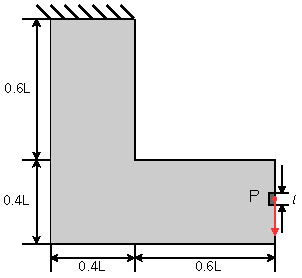
\includegraphics[
								width=0.94\linewidth,
								height=0.40\paperheight,
								keepaspectratio]{lbracket_bc}
								
				\end{tcolorbox}
				
			\end{column}
			
			% ─── 右栏：算例特征与参数设置 ─────────────────
			\begin{column}{0.485\linewidth}
				\begin{tcolorbox}[
					colback=white,
					colframe=structure.fg!55,
					colbacktitle=structure.fg,
					coltitle=white,
					fonttitle=\fontsize{8.2}{10}\selectfont\bfseries\sffamily,
					title={02\quad 算例参数与应力特征},
					arc=3pt,
					boxrule=0.5pt,
					toptitle=0.3pt,
					bottomtitle=0.3pt,
					top=6pt, bottom=5pt, left=9pt, right=9pt,
					height=0.50\paperheight]
					
					{\fontsize{7.55}{10.6}\selectfont\sffamily
						\setbeamertemplate{itemize item}{\raisebox{1pt}{\tiny$\bullet$}}
						\setlength{\leftmargini}{0.95em}
						\begin{itemize}
							\setlength{\itemsep}{4pt}
							\setlength{\topsep}{1pt}
							\setlength{\parsep}{0pt}
							\setlength{\parskip}{0pt}
							\item 外包围尺寸取 $L=200\,\mathrm{mm}$，水平臂与垂直臂宽度均为 $2L/5$。
							\item 左侧垂直臂顶端全固支，右侧水平臂末端中点施加竖向向下载荷 $P=400\,\mathrm{N}$。
							\item 材料参数取 $E=70000\,\mathrm{MPa}$，$\nu=0.25$ 和 $\bar{\sigma}=100\,\mathrm{MPa}$。
							\item 内凹角区域是典型的局部应力集中源。
							\item 用于考察应力约束对凹角应力集中区域的调控效果。
						\end{itemize}
						
					}
					
				\end{tcolorbox}
				
			\end{column}
			
		\end{columns}
		
	\end{frame}
	
	% ============================================================
	%  04-12  多分辨率框架在应力约束问题中的应用
	% ============================================================
	
	\begin{frame}
		\frametitle{多分辨率框架在应力约束问题中的应用}
		
		% ── 引导语 ───────────────────────────────────────────────
		\begin{tcolorbox}[
			colback=structure.fg!8, colframe=structure.fg!40,
			arc=2pt, boxrule=0.4pt,
			top=3pt, bottom=3pt, left=8pt, right=8pt]
			{\fontsize{8}{11}\selectfont\sffamily
				以 L 型支架为例，在多分辨率框架下比较不同有限元阶次对应力约束体积最小化结果的影响。}
		\end{tcolorbox}
		
		%		\vspace{0.5em}
		
		% ── 双主列嵌套布局 ───────────────────────────────────────
		\begin{columns}[T, totalwidth=\linewidth]
			
			% ════════════ 左主列：最终优化拓扑构型 ════════════
			\begin{column}{0.48\linewidth}\centering
				{\fontsize{9}{11}\selectfont\sffamily\bfseries\color{structure.fg}
					最终优化拓扑构型\par}
				
				% 嵌套子列：并排展示 k=1 和 k=4
				\begin{columns}[T, totalwidth=\linewidth]
					\begin{column}{0.48\linewidth}\centering
						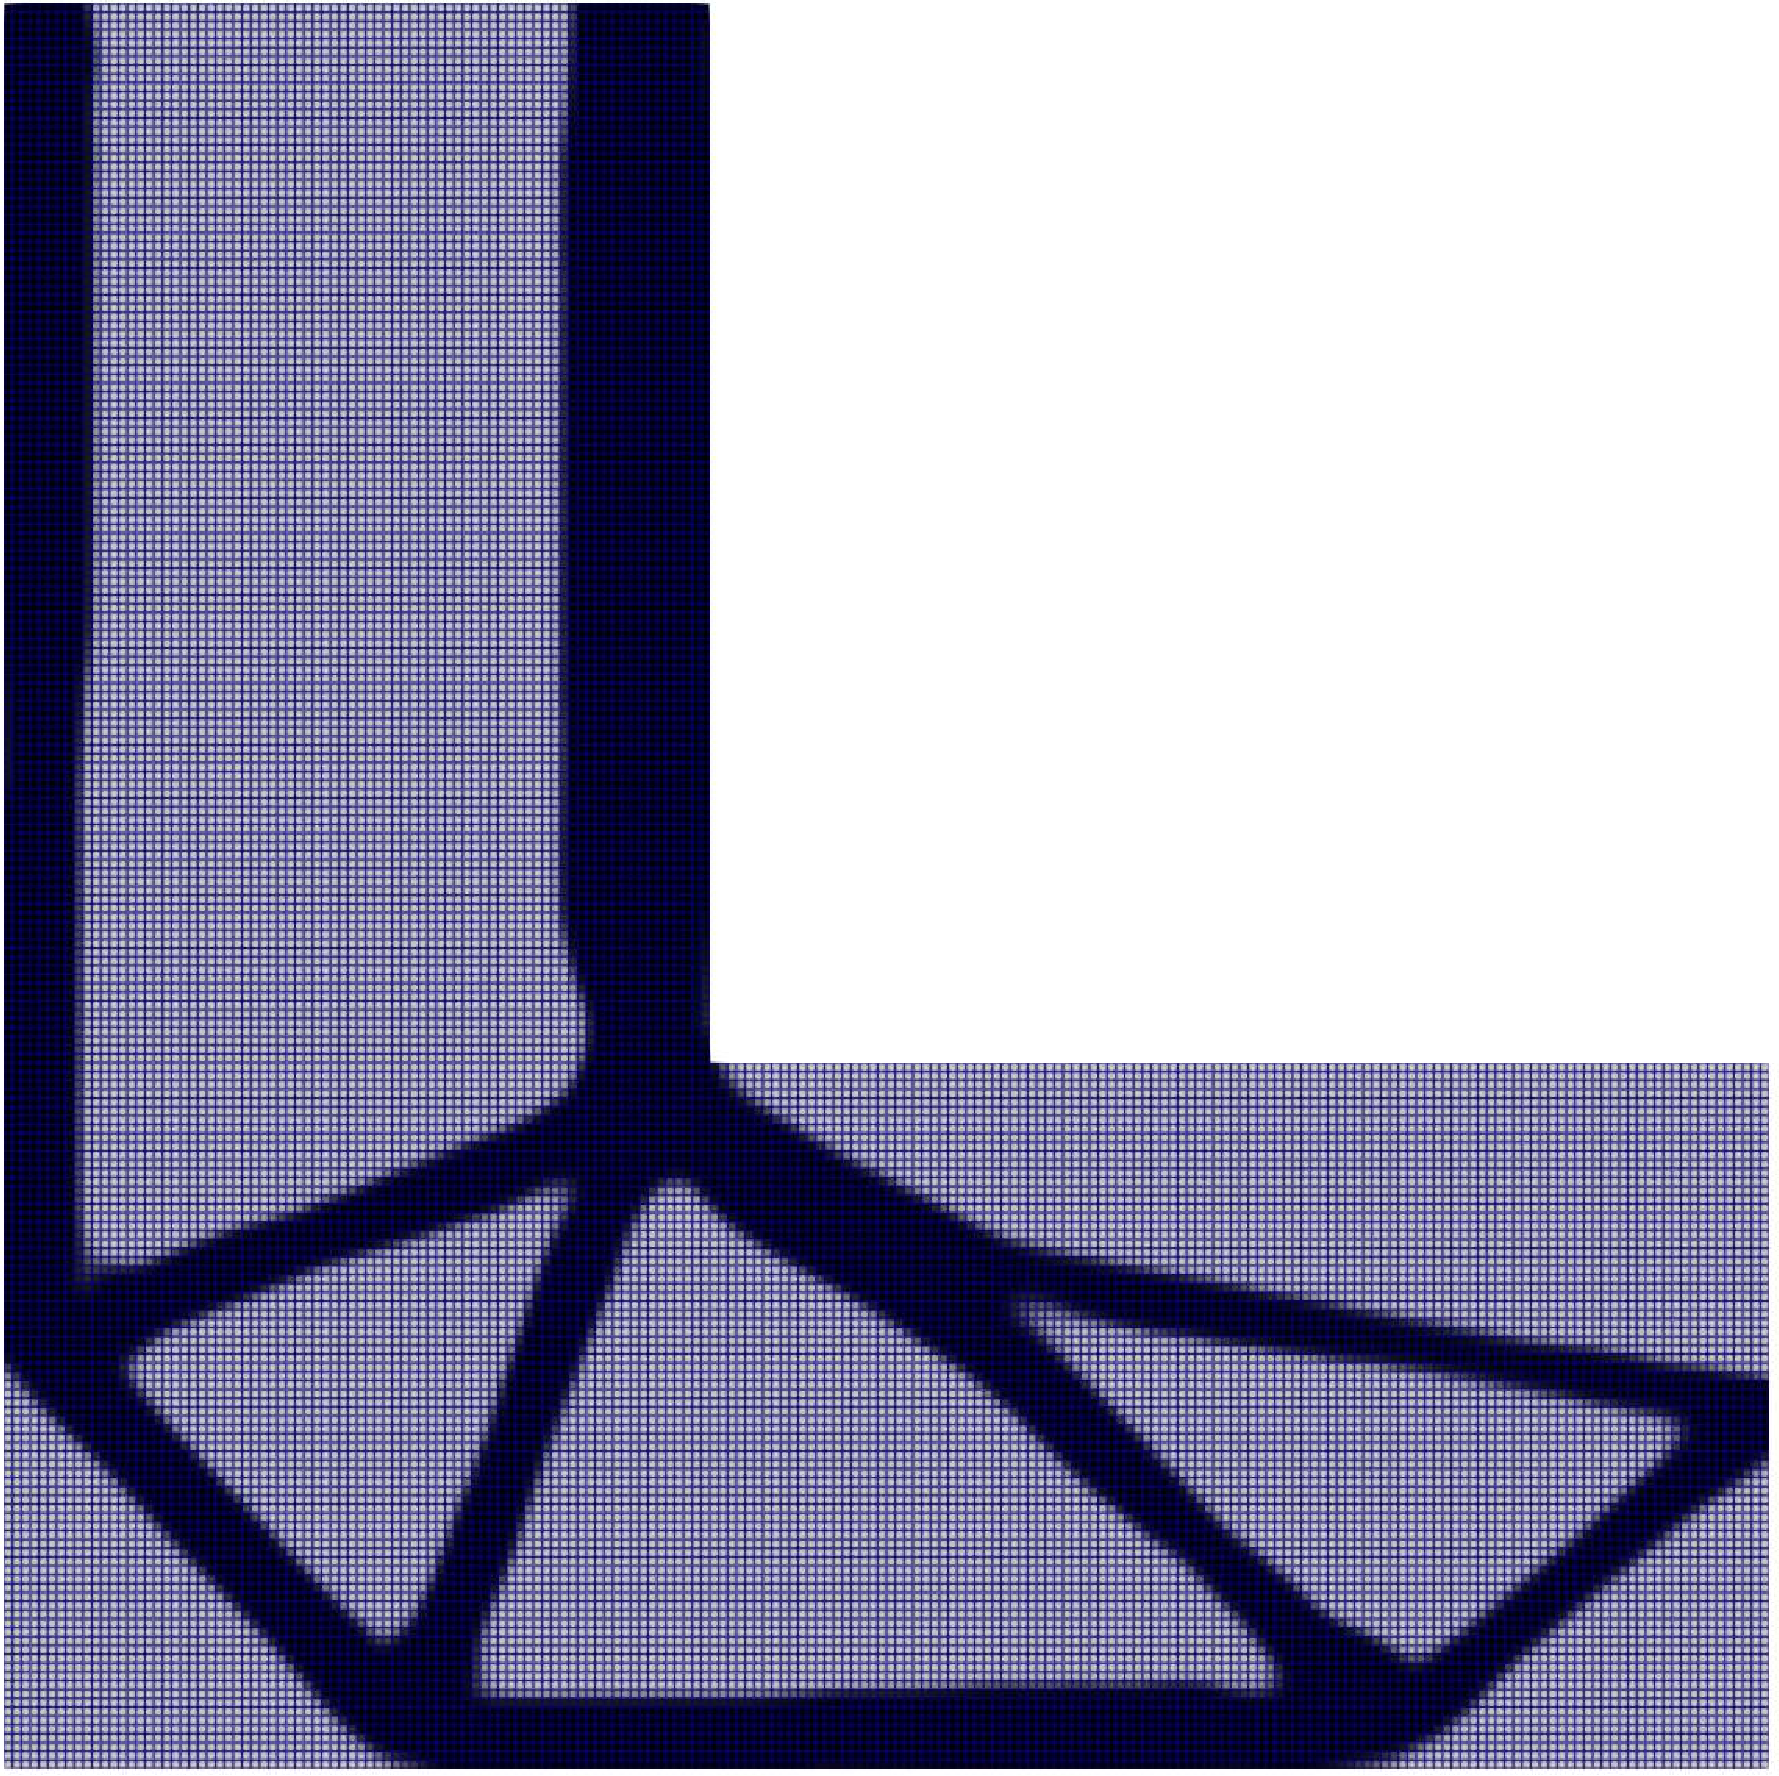
\includegraphics[width=\linewidth, keepaspectratio]{lbracket_topo_k1}\vspace{2pt}
						{\fontsize{8}{10}\selectfont\sffamily $k=1,r_{\min}=10.0$\par}
					\end{column}
					\begin{column}{0.48\linewidth}\centering
						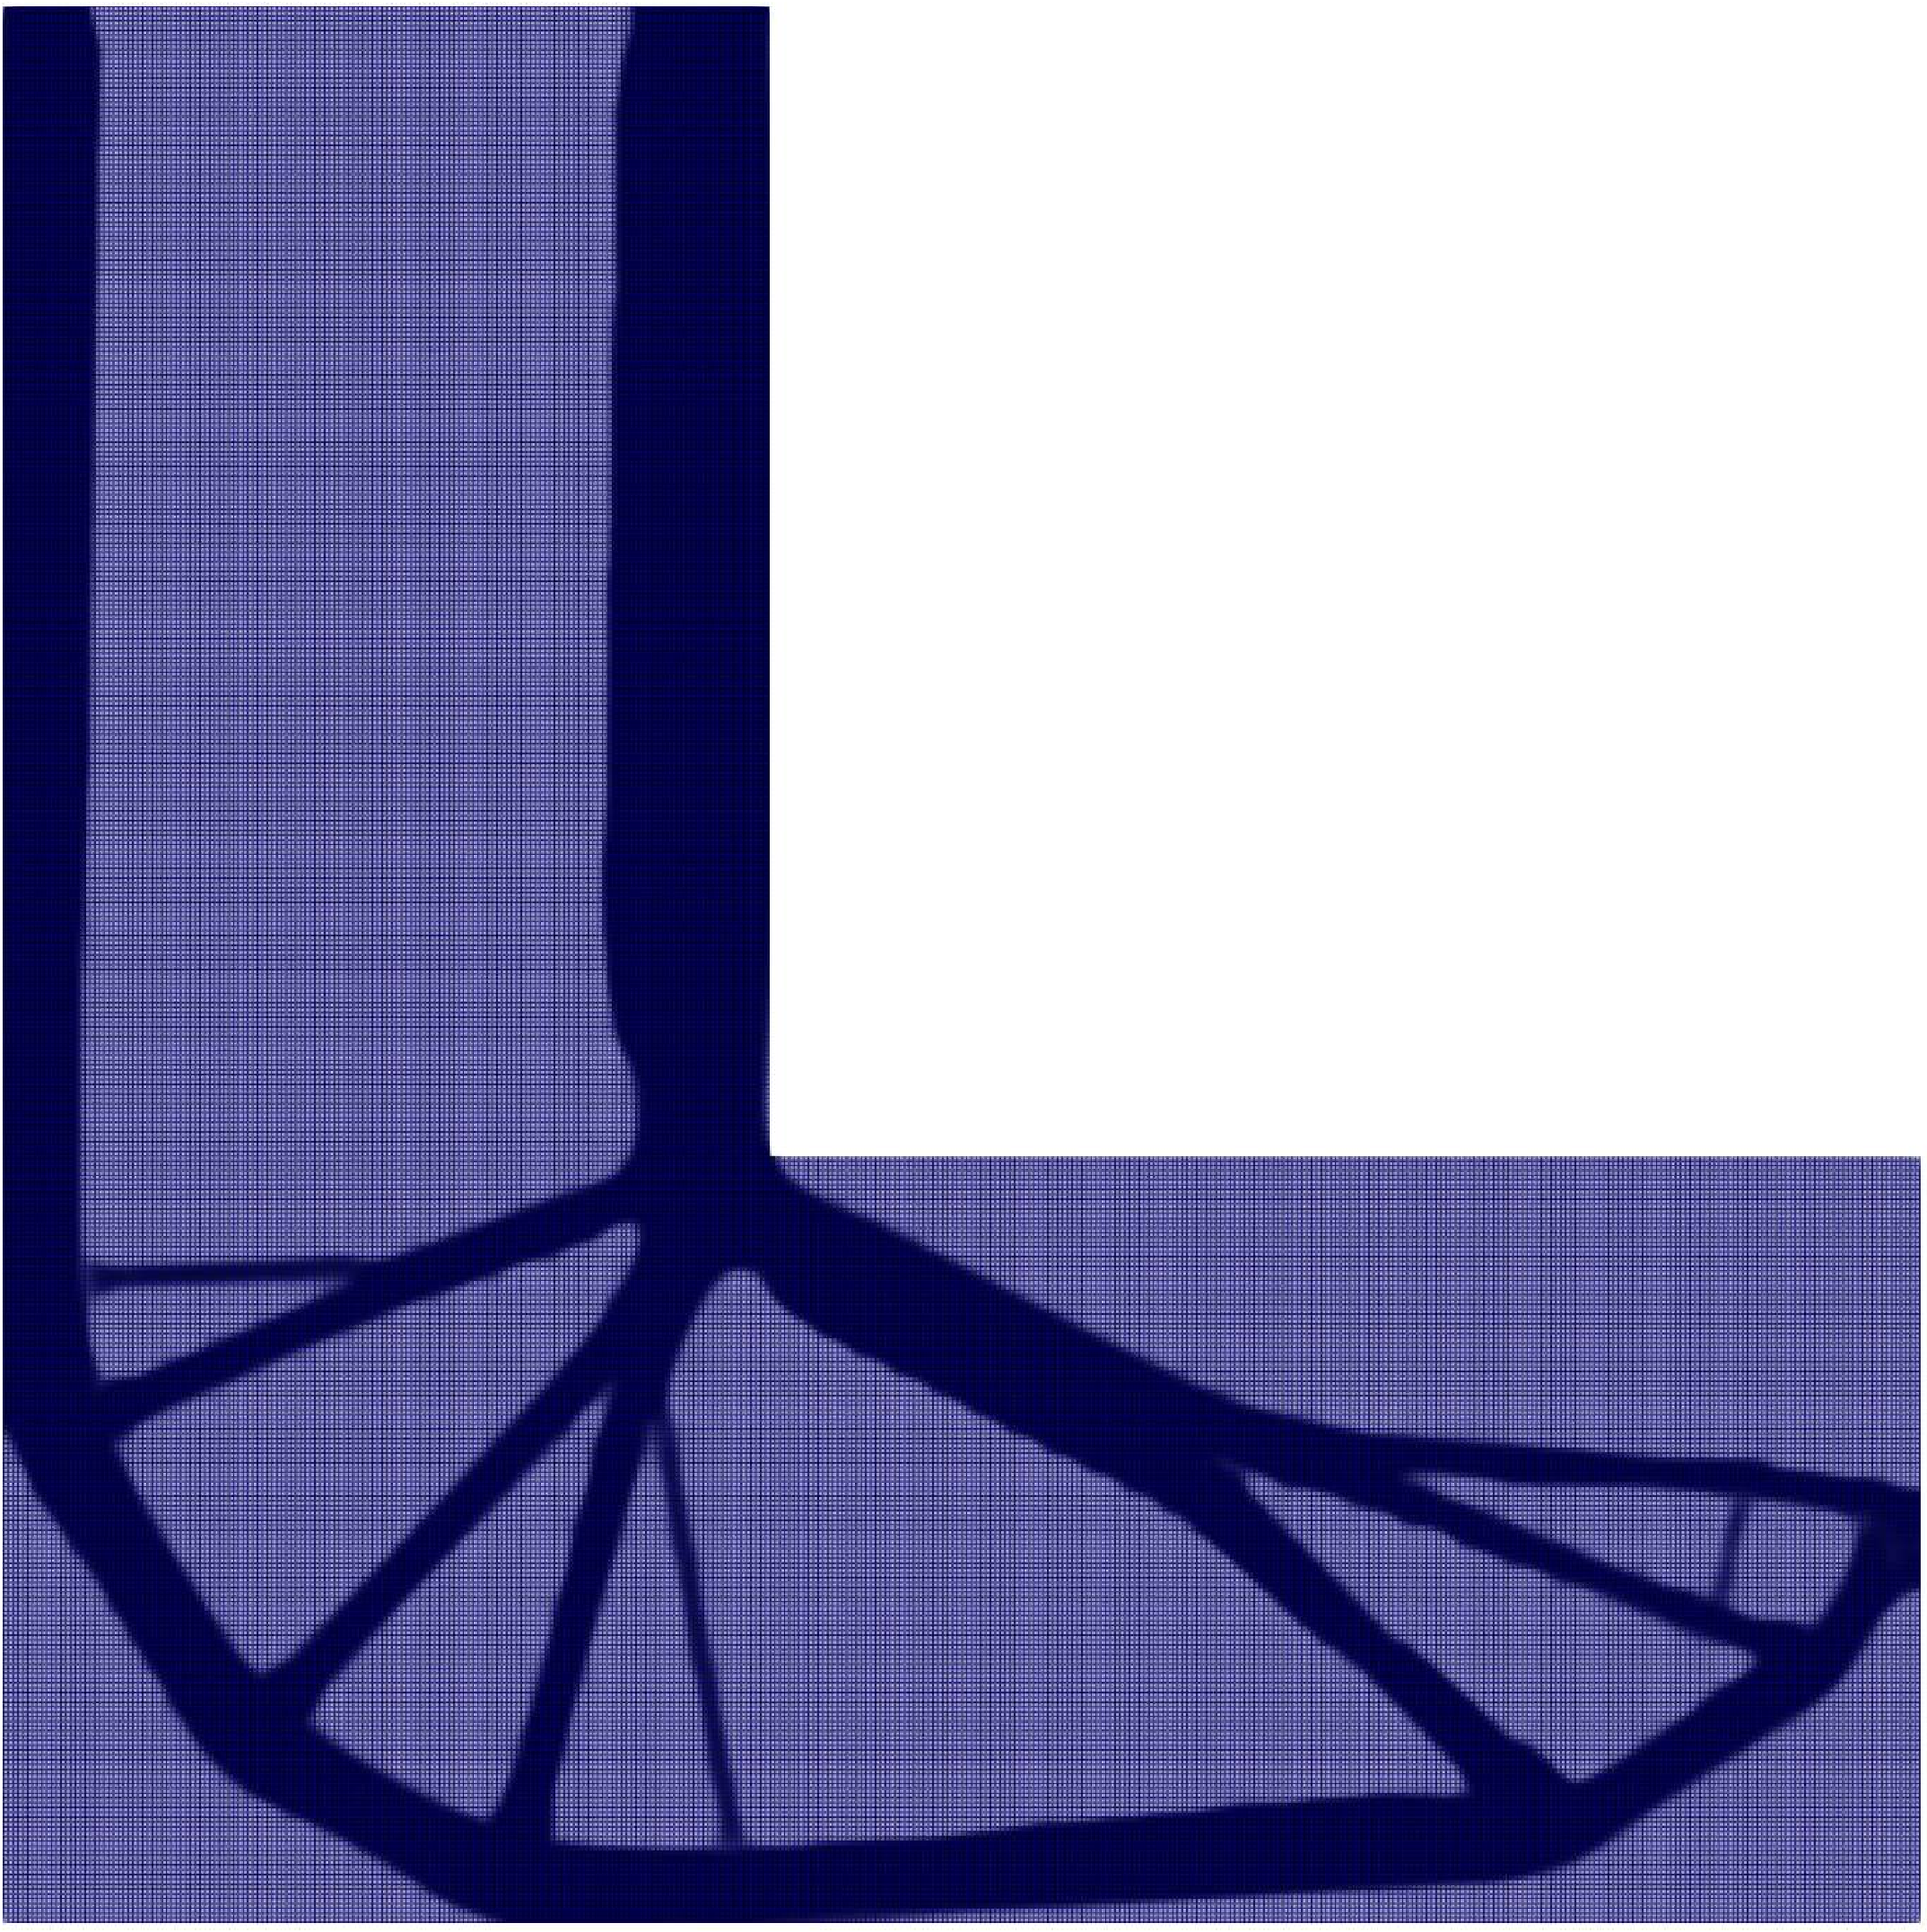
\includegraphics[width=\linewidth, keepaspectratio]{lbracket_topo_k4}\vspace{2pt}
						{\fontsize{8}{10}\selectfont\sffamily $k=4,r_{\min}=5.0$\par}
					\end{column}
				\end{columns}
			\end{column}
			
			% 中间间距
			\begin{column}{0.02\linewidth}\end{column}
			
			% ════════════ 右主列：归一化 von Mises 等效应力 ════════════
			\begin{column}{0.48\linewidth}\centering
				{\fontsize{9}{11}\selectfont\sffamily\bfseries\color{structure.fg}
					归一化 von Mises 等效应力\par}
				
				% 嵌套子列：并排展示 k=1 和 k=4
				\begin{columns}[T, totalwidth=\linewidth]
					\begin{column}{0.48\linewidth}\centering
						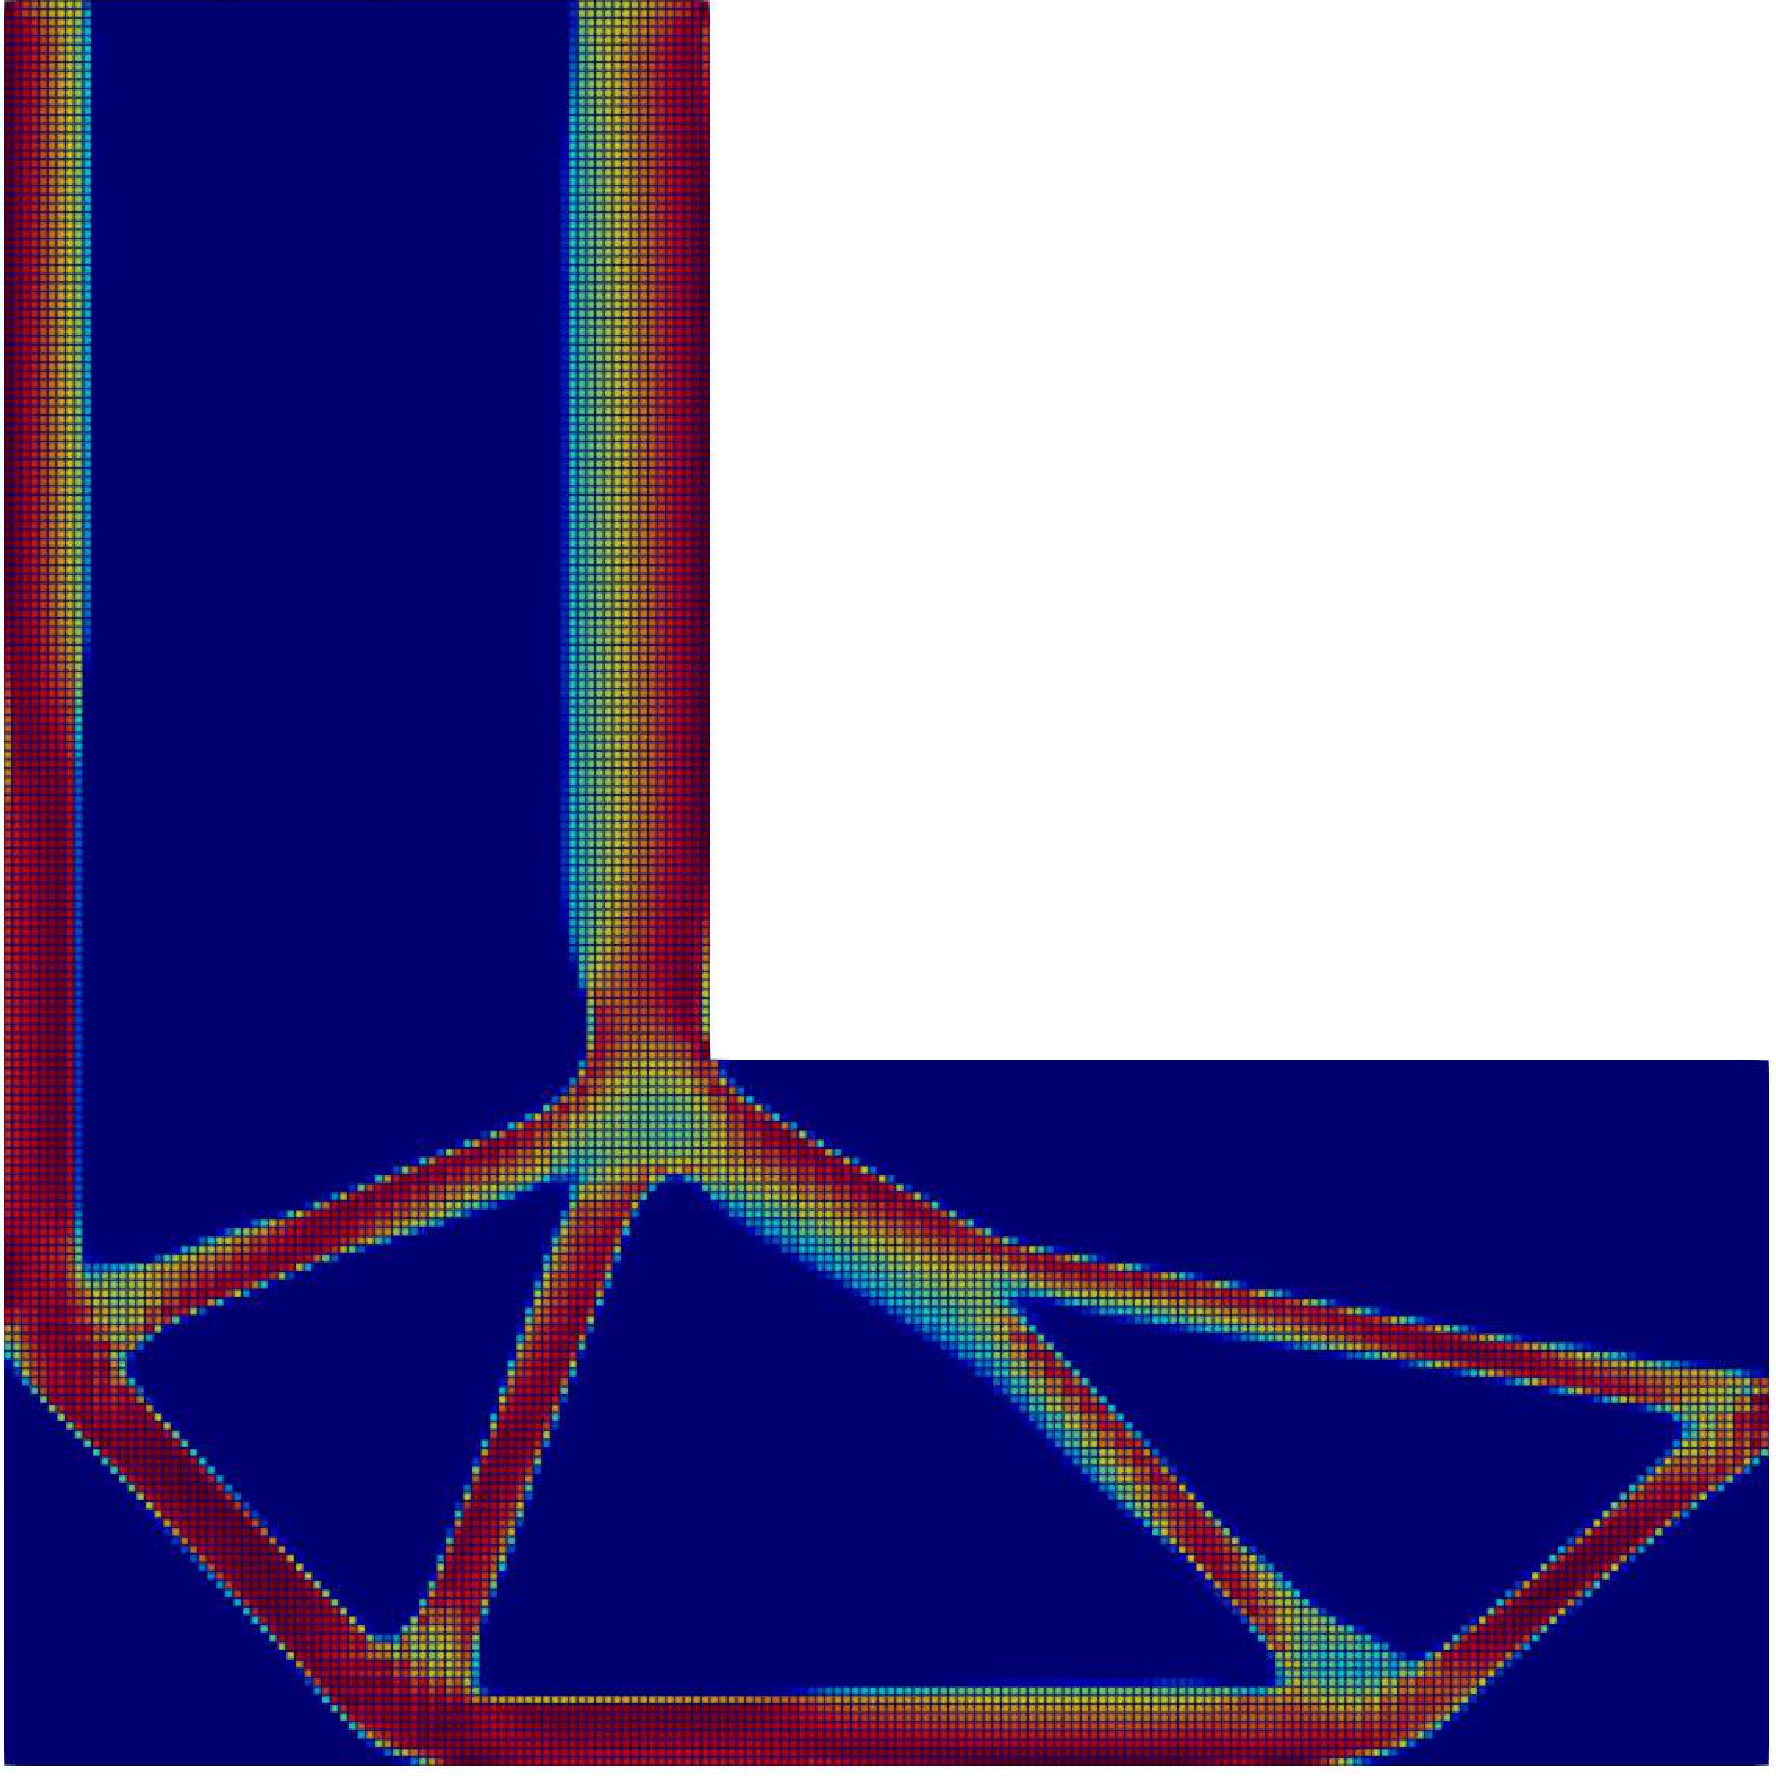
\includegraphics[width=\linewidth, keepaspectratio]{lbracket_stress_k1}\vspace{2pt}
						{\fontsize{8}{10}\selectfont\sffamily $k=1,r_{\min}=10.0$\par}
					\end{column}
					\begin{column}{0.48\linewidth}\centering
						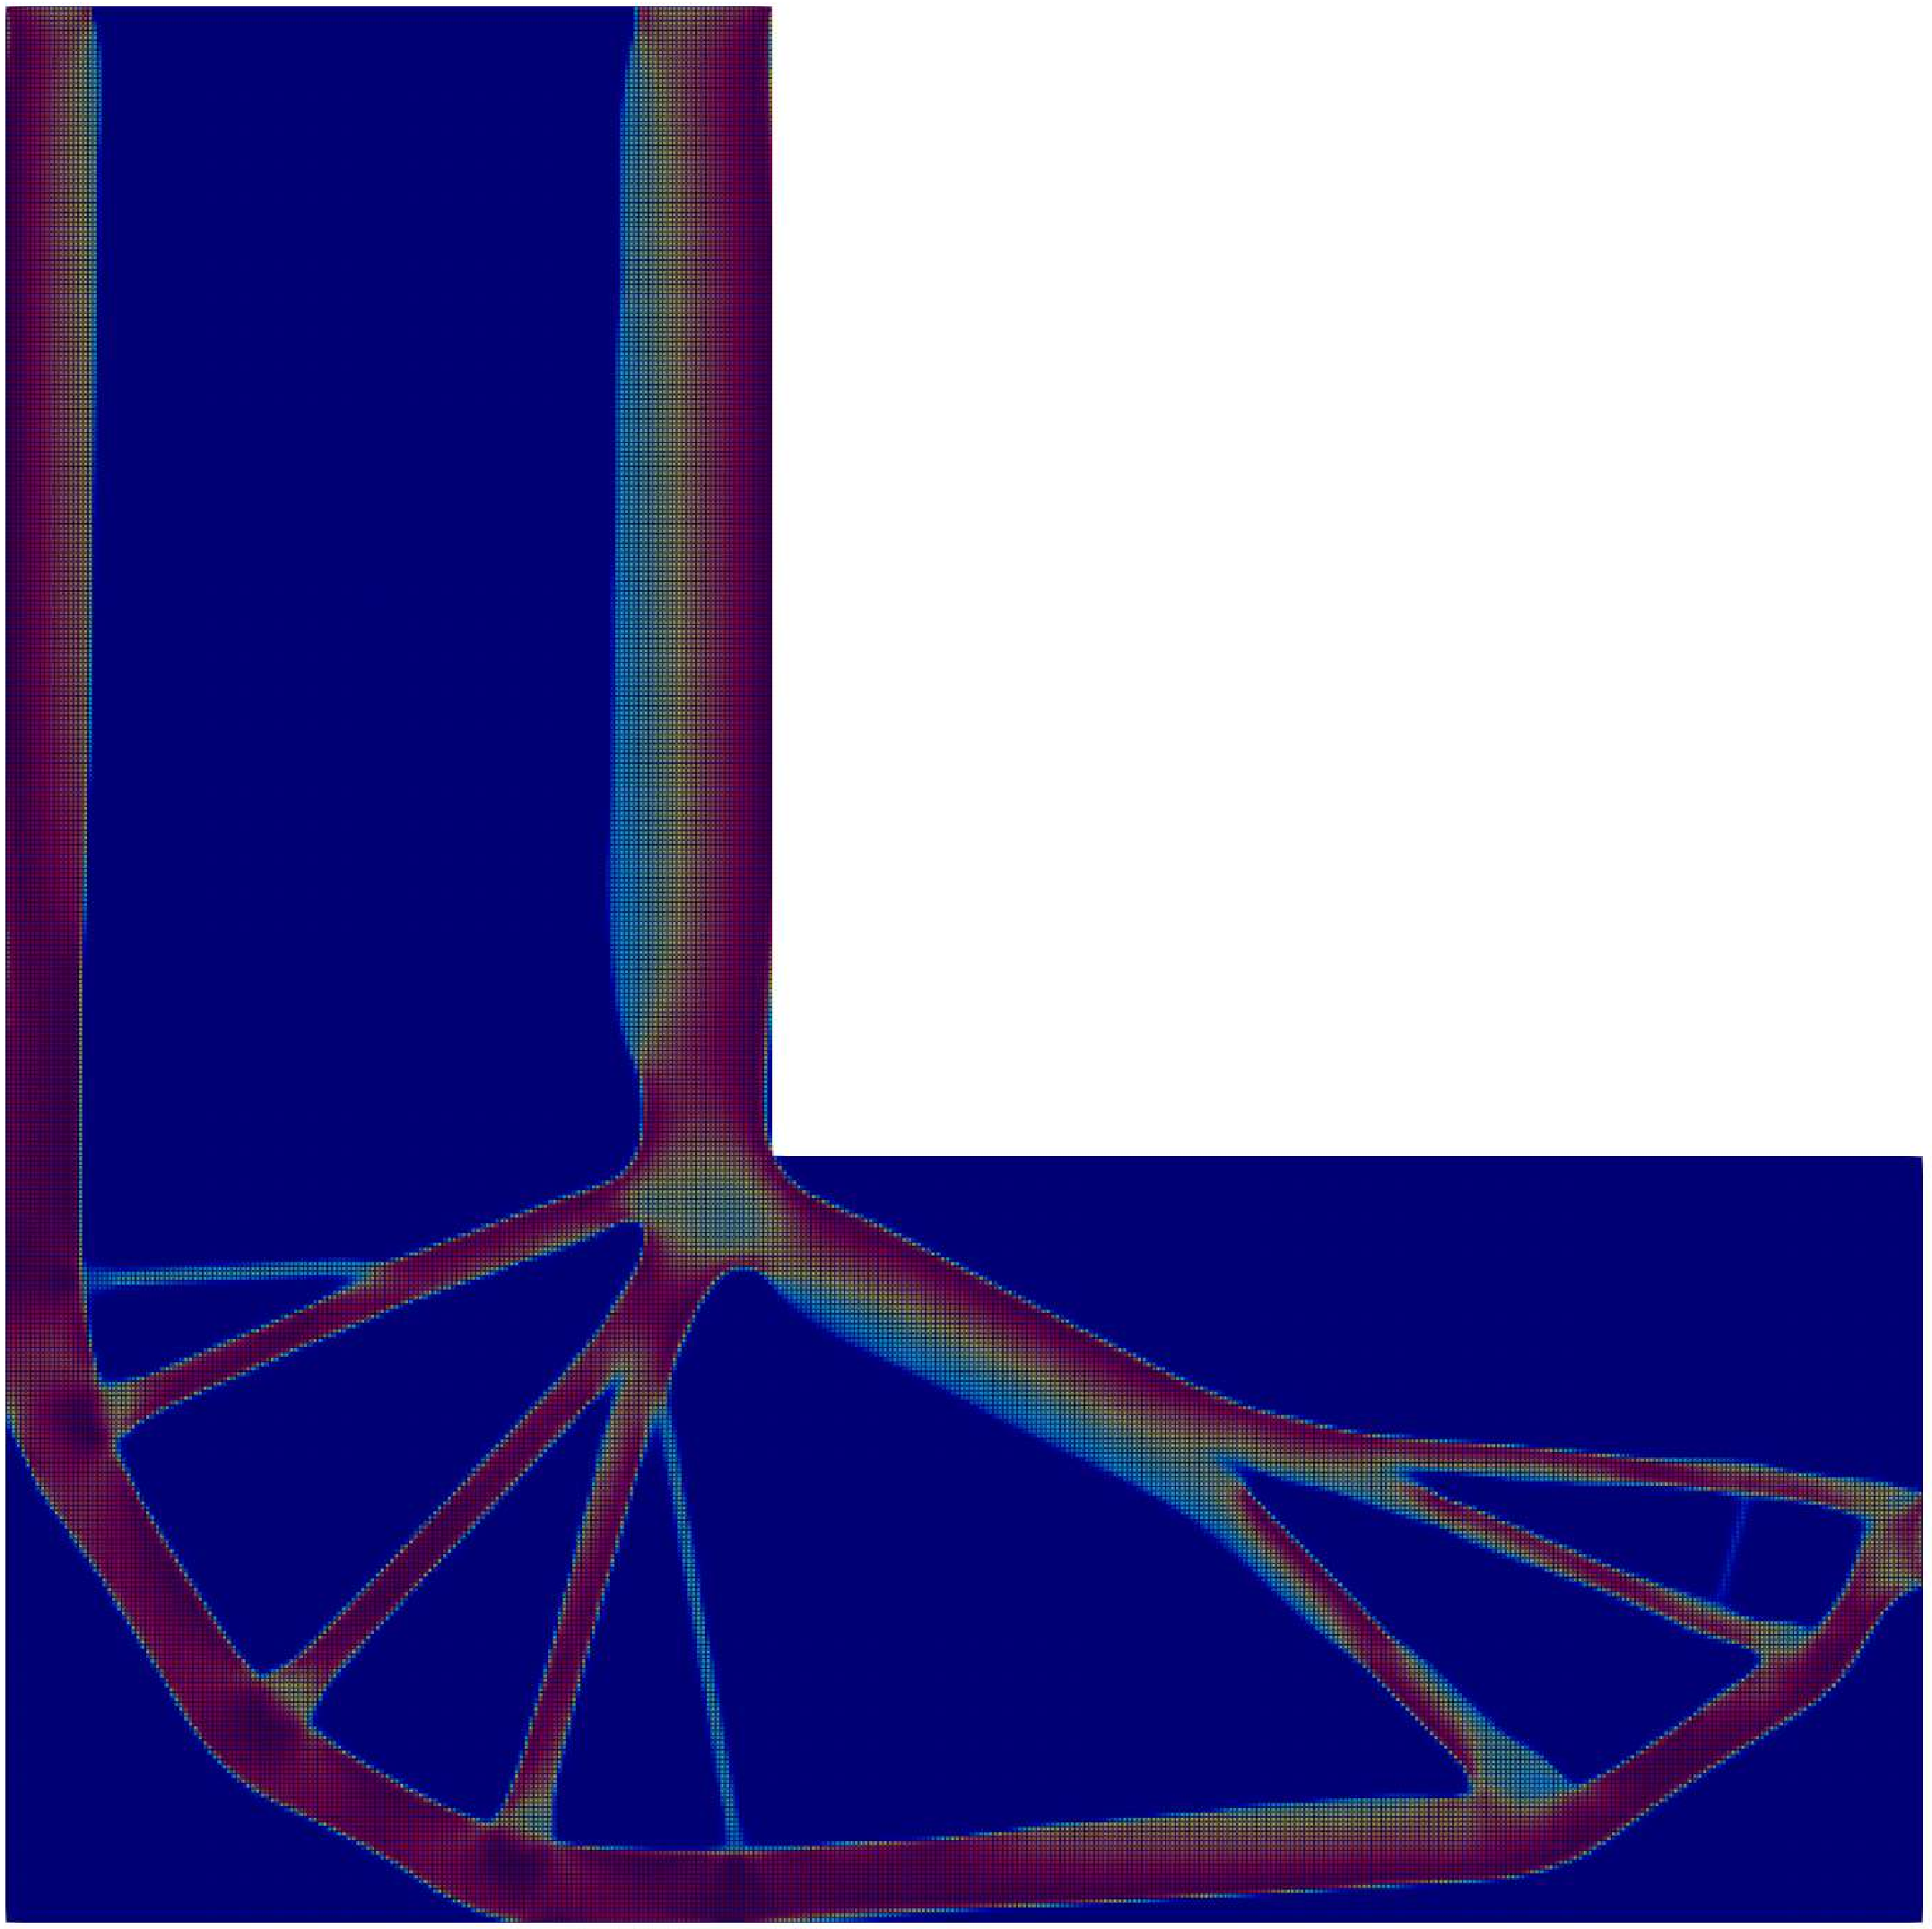
\includegraphics[width=\linewidth, keepaspectratio]{lbracket_stress_k4}\vspace{2pt}
						{\fontsize{8}{10}\selectfont\sffamily $k=4,r_{\min}=5.0$\par}
					\end{column}
				\end{columns}
			\end{column}
			
		\end{columns}
		
		\vspace{1em}
		
		% ── 底部结论条 ───────────────────────────────────────────
		\begin{tcolorbox}[
			colback=structure.fg, colframe=structure.fg,
			arc=3pt, boxrule=0pt,
			top=4pt, bottom=4pt, left=8pt, right=8pt]
			\centering
			{\fontsize{8}{11}\selectfont\sffamily\color{white}
				多分辨率框架可用于 L 型支架局部应力约束优化；
				进一步提升应力场逼近质量，需要引入混合有限元方法}
		\end{tcolorbox}
		
	\end{frame}
	
	
	% ============================================================
	\section{任意次胡张混合有限元拓扑优化方法}
	% ============================================================
	
	% ============================================================
	%  05-1  从位移法到混合应力建模：问题动机
	% ============================================================
	
	\begin{frame}
		\frametitle{从位移法到混合应力建模：问题动机}
		
		\vspace{-0.2em}
		
		% ── 顶部引导语 ───────────────────────────────────────────────
		\begin{tcolorbox}[
			colback=structure.fg!8, colframe=structure.fg!40,
			arc=2pt, boxrule=0.4pt,
			top=3pt, bottom=3pt, left=8pt, right=8pt]
			{\fontsize{8}{11}\selectfont\sffamily
				高阶有限元与多分辨率框架提升了位移场分析精度；
				但在近不可压缩材料和局部应力约束中，
				仍需更可靠的应力场建模方法。}
		\end{tcolorbox}
		
		\vspace{-1.0em}
		
		% ── 主体双栏 ───────────────────────────────────────────────
		\begin{columns}[T, totalwidth=\linewidth]
			
			% ════════ 左栏：近不可压缩材料中的体积闭锁 ════════
			\begin{column}{0.485\linewidth}
				\begin{tcolorbox}[
					colback=white, colframe=structure.fg!50,
					colbacktitle=structure.fg, coltitle=white,
					fonttitle=\fontsize{8}{10}\selectfont\bfseries\sffamily,
					title={近不可压缩材料中的体积闭锁},
					arc=3pt, boxrule=0.5pt,
					toptitle=3pt, bottomtitle=3pt,
					top=5pt, bottom=5pt, left=7pt, right=7pt,
					height=0.48\paperheight, valign=top]
					{\fontsize{7.25}{10.2}\selectfont\sffamily
						
						\textbf{\circnum{01}\enspace 材料极限情形}\par
						
						\vspace{2pt}
						
						当 $\nu\to 0.5$ 时，拉梅参数趋于无穷：
						
						\vspace{-2pt}
						
						\[
						\lambda
						=
						\frac{E\nu}{(1+\nu)(1-2\nu)}
						\ \longrightarrow\ \infty .
						\]
						
						\vspace{-2pt}
						
						\textbf{\circnum{02}\enspace 位移型有限元局限}\par
						
						\vspace{2pt}
						
						位移型有限元易出现体积闭锁，
						表现为数值刚度高估、位移场被过度约束，
						并影响拓扑演化。
					}
				\end{tcolorbox}
			\end{column}
			
			% ════════ 右栏：局部应力场评估的局限 ════════
			\begin{column}{0.485\linewidth}
				\begin{tcolorbox}[
					colback=white, colframe=structure.fg!50,
					colbacktitle=structure.fg, coltitle=white,
					fonttitle=\fontsize{8}{10}\selectfont\bfseries\sffamily,
					title={局部应力场评估的局限},
					arc=3pt, boxrule=0.5pt,
					toptitle=3pt, bottomtitle=3pt,
					top=5pt, bottom=5pt, left=7pt, right=7pt,
					height=0.48\paperheight, valign=top]
					{\fontsize{7.25}{10.2}\selectfont\sffamily
						
						\textbf{\circnum{01}\enspace 应力由位移梯度后处理}\par
						
						\vspace{2pt}
						
						位移型有限元中，应力由离散位移导出：
						
						\vspace{-12pt}
						
						\[
						\boldsymbol{\sigma}_h
						=
						\mathbb{C}(\rho):
						\boldsymbol{\varepsilon}(\boldsymbol{u}_h),
						\quad
						\boldsymbol{\varepsilon}(\boldsymbol{u}_h)
						=
						\tfrac12
						(\nabla\boldsymbol{u}_h+\nabla\boldsymbol{u}_h^{T}).
						\]
						
						\vspace{-4pt}
						
						\textbf{\circnum{02}\enspace 局部约束评估受限}\par
						
						\vspace{2pt}
						由于 $\boldsymbol{\sigma}_h$ 依赖
						$\nabla\boldsymbol{u}_h$，
						跨单元通常不连续；
						应力集中区域的局部约束评估精度受限。
					}
				\end{tcolorbox}
			\end{column}
			
		\end{columns}
		
		% ── 底部结论条 ───────────────────────────────────────────
		\begin{tcolorbox}[
			colback=structure.fg, colframe=structure.fg,
			arc=3pt, boxrule=0pt,
			top=3pt, bottom=3pt, left=8pt, right=8pt]
			\centering
			{\fontsize{7.8}{11}\selectfont\sffamily\color{white}
				位移法以 $\boldsymbol{u}_h$ 为主变量、应力场依赖后处理；
				混合应力建模是提升局部应力评估可靠性的关键。}
		\end{tcolorbox}
		
	\end{frame}
	
	% ============================================================
	%  05-2  从位移导出应力到应力--位移混合求解
	%        Overlay 1: 强形式 / Overlay 2: 弱形式
	% ============================================================
	
	\begin{frame}
		\frametitle{从位移导出应力到应力--位移混合求解}
		
		% ── 顶部引导语 ───────────────────────────────────────────────
		\begin{tcolorbox}[
			colback=structure.fg!8, colframe=structure.fg!40,
			arc=2pt, boxrule=0.4pt,
			top=3pt, bottom=3pt, left=8pt, right=8pt]
			{\fontsize{8}{11}\selectfont\sffamily
				为避免应力场完全依赖位移梯度后处理，
				引入 Hellinger--Reissner 混合变分原理，
				将应力 $\boldsymbol{\sigma}$ 与位移 $\boldsymbol{u}$ 同时作为未知量求解。}
		\end{tcolorbox}
		
		% ============================================================
		% Overlay 1：应力--位移混合强形式
		% ============================================================
		\only<1>{
			\begin{tcolorbox}[
				colback=white, colframe=structure.fg!50,
				colbacktitle=structure.fg, coltitle=white,
				fonttitle=\fontsize{8}{10}\selectfont\bfseries\sffamily,
				title={\circnum{01}\enspace 应力--位移混合强形式},
				arc=3pt, boxrule=0.5pt,
				toptitle=3pt, bottomtitle=3pt,
				top=8pt, bottom=6pt, left=12pt, right=12pt,
				height=0.52\paperheight, valign=top]
				{\fontsize{7.65}{10.6}\selectfont\sffamily
					
					\vspace{0.15em}
					
					\begin{columns}[T, totalwidth=\linewidth]
						
						% ── 左侧：本构关系与柔度算子 ─────────────────────
						\begin{column}{0.48\linewidth}
							\centering
							{\fontsize{7.6}{9.6}\selectfont\bfseries\sffamily
								本构互逆关系}
							
							\vspace{-1.5em}
							
							\[
							\mathcal{A}
							=
							\mathbb{C}^{-1},
							\qquad
							\boldsymbol{\varepsilon}(\boldsymbol{u})
							=
							\mathcal{A}\boldsymbol{\sigma},
							\qquad
							\boldsymbol{\sigma}
							=
							\mathbb{C}:
							\boldsymbol{\varepsilon}(\boldsymbol{u}).
							\]
							
							\vspace{-0.15em}
							
							{\fontsize{7.6}{9.6}\selectfont\bfseries\sffamily
								各向同性材料下的柔度算子}
							
							\vspace{-1.5em}
							
							\[
							\mathcal{A}\boldsymbol{\tau}
							=
							\frac{1}{2\mu}
							\left(
							\boldsymbol{\tau}
							-
							\frac{\lambda}{2\mu+d\lambda}
							\operatorname{tr}(\boldsymbol{\tau})\boldsymbol{I}
							\right),
							\qquad
							\forall\,\boldsymbol{\tau}\in\mathbb{S}.
							\]
						\end{column}
						
						% ── 右侧：混合强形式 ─────────────────────────────
						\begin{column}{0.48\linewidth}
							\centering
							{\fontsize{7.6}{9.6}\selectfont\bfseries\sffamily
								混合强解 $(\boldsymbol{\sigma},\boldsymbol{u})$ 满足}
							
							\vspace{-1.5em}
							
							\[
							\left\{
							\begin{aligned}
								-\operatorname{div}\boldsymbol{\sigma}
								&=
								\boldsymbol{b},
								&& \text{in } \Omega,
								\\[3pt]
								\mathcal{A}\boldsymbol{\sigma}
								&=
								\boldsymbol{\varepsilon}(\boldsymbol{u}),
								&& \text{in } \Omega,
								\\[3pt]
								\boldsymbol{u}
								&=
								\boldsymbol{u}_{D},
								&& \text{on } \Gamma_D,
								\\[3pt]
								\boldsymbol{\sigma}\boldsymbol{n}
								&=
								\boldsymbol{g},
								&& \text{on } \Gamma_N .
							\end{aligned}
							\right.
							\]
						\end{column}
						
					\end{columns}
					
					\vspace{1.0em}
					
					{\fontsize{7.15}{9.6}\selectfont
						其中，$\mathcal{A}$ 为柔度算子；
						应力张量 $\boldsymbol{\sigma}$ 作为主要未知量，
						与位移 $\boldsymbol{u}$ 共同描述线弹性体的内部力学状态。}
				}
			\end{tcolorbox}
			
			\begin{tcolorbox}[
				colback=structure.fg, colframe=structure.fg,
				arc=3pt, boxrule=0pt,
				top=3pt, bottom=3pt, left=8pt, right=8pt]
				\centering
				{\fontsize{8.0}{11}\selectfont\sffamily\color{white}
					混合强形式通过平衡方程与柔度型本构关系，刻画应力场与位移场的耦合。}
			\end{tcolorbox}
		}
		
		% ============================================================
		% Overlay 2：Hellinger--Reissner 混合弱形式
		% ============================================================
		\only<2>{
			\begin{tcolorbox}[
				colback=white, colframe=structure.fg!50,
				colbacktitle=structure.fg, coltitle=white,
				fonttitle=\fontsize{8}{10}\selectfont\bfseries\sffamily,
				title={\circnum{02}\enspace Hellinger--Reissner 混合弱形式},
				arc=3pt, boxrule=0.5pt,
				toptitle=3pt, bottomtitle=3pt,
				top=8pt, bottom=6pt, left=12pt, right=12pt,
				height=0.50\paperheight, valign=top]
				{\fontsize{7.65}{10.6}\selectfont\sffamily
					
					\vspace{0.15em}
					
					\centering
					{\fontsize{7.6}{9.6}\selectfont\bfseries\sffamily
						应力空间与位移空间：$\boldsymbol{\Sigma}
						=
						H(\operatorname{div};\Omega;\mathbb{S}),
						\quad
						\boldsymbol{V}
						=
						L^2(\Omega;\mathbb{R}^{d}).$
					}
					
					\vspace{1.5em}
					
					{\fontsize{7.6}{9.6}\selectfont\bfseries\sffamily
						混合弱形式：求
						$(\boldsymbol{\sigma},\boldsymbol{u})
						\in
						\boldsymbol{\Sigma}_{\boldsymbol{g}}
						\times
						\boldsymbol{V}$，
						使得对任意
						$(\boldsymbol{\tau},\boldsymbol{v})
						\in
						\boldsymbol{\Sigma}_{0}
						\times
						\boldsymbol{V}$，}
					
					\vspace{-1.5em}
					
					\[
					\left\{
					\begin{aligned}
						(\mathcal{A}\boldsymbol{\sigma},
						\boldsymbol{\tau})
						+
						(\operatorname{div}\boldsymbol{\tau},
						\boldsymbol{u})
						&=
						\langle
						\boldsymbol{u}_{D},
						\boldsymbol{\tau}\boldsymbol{n}
						\rangle_{\Gamma_D},
						\\[4pt]
						(\operatorname{div}\boldsymbol{\sigma},
						\boldsymbol{v})
						&=
						-(\boldsymbol{b},\boldsymbol{v}).
					\end{aligned}
					\right.
					\]
					
					{\fontsize{7.6}{9.6}\selectfont
						其中，$\boldsymbol{\Sigma}_{\boldsymbol{g}}$ 与 $\boldsymbol{\Sigma}_{0}$
						分别表示满足非齐次和齐次牵引边界条件的应力空间。}
				}
			\end{tcolorbox}

			\begin{tcolorbox}[
				colback=structure.fg, colframe=structure.fg,
				arc=3pt, boxrule=0pt,
				top=3pt, bottom=3pt, left=8pt, right=8pt]
				\centering
				{\fontsize{8.0}{11}\selectfont\sffamily\color{white}
					明确了应力空间的 $H(\operatorname{div})$ 协调要求，
					为构造胡张应力空间及相应混合有限元奠定基础。}
			\end{tcolorbox}
		}
		
	\end{frame}
	
	% ============================================================
	%  05-3  任意次胡张混合有限元方法
	%        Overlay 1: 应力空间 / Overlay 2: 位移空间与空间配对
	% ============================================================
	
	\begin{frame}
		\frametitle{任意次胡张混合有限元方法}

		% ── 顶部引导语 ───────────────────────────────────────────────
		\begin{tcolorbox}[
			colback=structure.fg!8, colframe=structure.fg!40,
			arc=2pt, boxrule=0.4pt,
			top=3pt, bottom=3pt, left=8pt, right=8pt]
			% ── 顶部引导语 ───────────────────────────────────────────────
			{\fontsize{8}{11}\selectfont\sffamily
				基于任意次单纯形 Hu--Zhang 元，构造满足
				$H(\operatorname{div})$ 协调性的对称张量值应力空间
				$\boldsymbol{\Sigma}_h^k$，
				并与低一阶全不连续位移空间 $\boldsymbol{V}_h^{k-1}$ 配对；
				标准格式主要适用于高阶情形。}
		\end{tcolorbox}
		
		\only<1>{
			\begin{tcolorbox}[
				colback=white, colframe=structure.fg!50,
				colbacktitle=structure.fg, coltitle=white,
				fonttitle=\fontsize{8}{10}\selectfont\bfseries\sffamily,
				title={\circnum{01}\enspace 单纯形胡张应力空间构造},
				arc=3pt, boxrule=0.5pt,
				toptitle=3pt, bottomtitle=3pt,
				top=7pt, bottom=6pt, left=12pt, right=12pt,
				height=0.47\paperheight, valign=center]
				{\fontsize{7.55}{10.4}\selectfont\sffamily
					
					\centering
					{\fontsize{7.9}{10}\selectfont\bfseries\sffamily
						全局离散胡张应力空间}
					
					\vspace{-0.75em}
					
					\[
					\boldsymbol{\Sigma}_h^k
					:=
					\left\{
					\begin{aligned}
						\boldsymbol{\sigma}_h\in L^2(\Omega;\mathbb{S})\ :\ 
						&\boldsymbol{\sigma}_h|_T\in P_k(T;\mathbb{S}),
						\quad \forall T\in\mathcal{T}_h,\\[-1pt]
						&\mathcal{N}\text{-型自由度在共享 }(d-1)\text{-面上单值}
					\end{aligned}
					\right\}.
					\]
					
					\vspace{-0.35em}
					
					{\fontsize{7.9}{10}\selectfont\bfseries\sffamily
						协调性机制}
					
					\vspace{-1.35em}
					
					\[
					\mathcal{N}\text{-型自由度单值}
					\Longrightarrow
					\boldsymbol{\sigma}_h\boldsymbol{n}\text{ 的法向迹连续}
					\Longrightarrow
					\boldsymbol{\Sigma}_h^k
					\subset
					H(\operatorname{div};\Omega;\mathbb{S}).
					\]
				}
			\end{tcolorbox}
			
			\vspace{-0.15em}
			
			\begin{tcolorbox}[
				colback=structure.fg, colframe=structure.fg,
				arc=3pt, boxrule=0pt,
				top=3pt, bottom=3pt, left=8pt, right=8pt]
				\centering
				{\fontsize{8.0}{11}\selectfont\sffamily\color{white}
					核心是通过法向迹连续性，构造 $H(\operatorname{div})$ 协调的对称应力空间。}
			\end{tcolorbox}
		}
	
		% ============================================================
		% Overlay 2：位移空间选取与高阶稳定配对
		% ============================================================
		\only<2>{
			\begin{tcolorbox}[
				colback=white, colframe=structure.fg!50,
				colbacktitle=structure.fg, coltitle=white,
				fonttitle=\fontsize{8}{10}\selectfont\bfseries\sffamily,
				title={\circnum{02}\enspace 位移空间选取与高阶稳定配对},
				arc=3pt, boxrule=0.5pt,
				toptitle=3pt, bottomtitle=3pt,
				top=6pt, bottom=6pt, left=12pt, right=12pt,
				height=0.47\paperheight, valign=center]
				{\fontsize{7.45}{10.3}\selectfont\sffamily
					
					\centering
					{\fontsize{7.8}{9.8}\selectfont\bfseries\sffamily
						低一阶全不连续位移空间}
					
					\vspace{-1.5em}
					
					\[
					\boldsymbol{V}_h^{k-1}
					:=
					\left\{
					\boldsymbol{v}_h\in L^2(\Omega;\mathbb{R}^{d})
					:
					\boldsymbol{v}_h|_T\in P_{k-1}(T;\mathbb{R}^{d}),
					\ \forall T\in\mathcal{T}_h
					\right\}.
					\]
					
					\vspace{-0.65em}
					
					\begin{columns}[T, totalwidth=\linewidth]
						
						\begin{column}{0.48\linewidth}
							{\fontsize{7.8}{9.8}\selectfont\bfseries\sffamily
								空间配对}
							
							\vspace{-0.9em}
							\[
							\boldsymbol{\Sigma}_h^k
							\times
							\boldsymbol{V}_h^{k-1}
							\]
							\vspace{-1.05em}
							
							{\fontsize{7.2}{9.4}\selectfont\sffamily
								应力空间承担跨单元法向牵引连续性，
								位移空间仅需 $L^2$ 离散。}
						\end{column}
						
						\begin{column}{0.48\linewidth}
							{\fontsize{7.8}{9.8}\selectfont\bfseries\sffamily
								离散 inf-sup 条件限制}
							
							\vspace{-0.9em}
							\[
							\boldsymbol{k\ge d+1}
							\]
							\vspace{-1.1em}
							
							低阶情形 $1\le k\le d$ 不满足离散 inf-sup 条件，
							因此需要在后续引入额外稳定化处理。
							
						\end{column}
						
					\end{columns}

				}
			\end{tcolorbox}
			
			\vspace{-0.15em}
			
			\begin{tcolorbox}[
				colback=structure.fg, colframe=structure.fg,
				arc=3pt, boxrule=0pt,
				top=3pt, bottom=3pt, left=8pt, right=8pt]
				\centering
				{\fontsize{8.0}{11}\selectfont\sffamily\color{white}
					标准 Hu--Zhang 混合配对主要适用于高阶情形，
					低阶应用需进一步引入稳定化扩展。}
			\end{tcolorbox}
		}
		
		% ============================================================
		% Overlay 3：离散混合变分格式
		% ============================================================
		\only<3>{
			\begin{tcolorbox}[
				colback=white, colframe=structure.fg!50,
				colbacktitle=structure.fg, coltitle=white,
				fonttitle=\fontsize{8}{10}\selectfont\bfseries\sffamily,
				title={\circnum{03}\enspace 离散混合变分格式},
				arc=3pt, boxrule=0.5pt,
				toptitle=3pt, bottomtitle=3pt,
				top=8pt, bottom=6pt, left=12pt, right=12pt,
				height=0.50\paperheight, valign=top]
				{\fontsize{7.65}{10.6}\selectfont\sffamily
					
					\vspace{0.15em}
					
					\centering
					{\fontsize{7.6}{9.6}\selectfont\bfseries\sffamily
						离散空间配对：
						$\boldsymbol{\Sigma}_h^{k}
						\subset
						H(\operatorname{div};\Omega;\mathbb{S}),
						\quad
						\boldsymbol{V}_h^{k-1}
						\subset
						L^2(\Omega;\mathbb{R}^{d}).$
					}
					
					\vspace{1.45em}
					
					{\fontsize{7.6}{9.6}\selectfont\bfseries\sffamily
						离散混合格式：求
						$(\boldsymbol{\sigma}_h,\boldsymbol{u}_h)
						\in
						\boldsymbol{\Sigma}_{h,g_N}^{k}
						\times
						\boldsymbol{V}_h^{k-1}$，
						使得对任意
						$(\boldsymbol{\tau}_h,\boldsymbol{v}_h)
						\in
						\boldsymbol{\Sigma}_{h,0}^{k}
						\times
						\boldsymbol{V}_h^{k-1}$，}
					
					\vspace{-1.45em}
					
					\[
					\left\{
					\begin{aligned}
						a(\boldsymbol{\sigma}_h,\boldsymbol{\tau}_h)
						+
						b(\boldsymbol{\tau}_h,\boldsymbol{u}_h)
						&=
						\ell(\boldsymbol{\tau}_h),
						\\[4pt]
						b(\boldsymbol{\sigma}_h,\boldsymbol{v}_h)
						&=
						f(\boldsymbol{v}_h).
					\end{aligned}
					\right.
					\]
					
					{\fontsize{7.6}{9.6}\selectfont
						其中，$\boldsymbol{\Sigma}_{h,g_N}^{k}$ 与
						$\boldsymbol{\Sigma}_{h,0}^{k}$
						分别表示满足非齐次和齐次牵引边界条件的离散应力空间。}
				}
			\end{tcolorbox}
			
			\begin{tcolorbox}[
				colback=structure.fg, colframe=structure.fg,
				arc=3pt, boxrule=0pt,
				top=3pt, bottom=3pt, left=8pt, right=8pt]
				\centering
				{\fontsize{8.0}{11}\selectfont\sffamily\color{white}
					该离散格式形成应力--位移混合鞍点系统，
					为低阶稳定化处理和拓扑优化列式奠定基础。}
			\end{tcolorbox}
		}
		
	\end{frame}
	
	% ============================================================
	%  05-4  复杂边界下顶点应力连续性部分松弛
	% ============================================================
	
	\begin{frame}
		\frametitle{复杂边界下顶点应力连续性部分松弛}
		
		\vspace{-0.25em}
		
		\begin{tcolorbox}[
			colback=structure.fg!8, colframe=structure.fg!40,
			arc=2pt, boxrule=0.4pt,
			top=2pt, bottom=2pt, left=8pt, right=8pt]
			{\fontsize{7.8}{10.5}\selectfont\sffamily
				复杂边界角点处若强制顶点应力完全连续，容易形成局部过约束；
				通过松弛切向相关自由度并保持法向迹单值，可兼顾复杂边界适配与
				$H(\operatorname{div})$ 协调性。}
		\end{tcolorbox}
		
		\vspace{-0.45em}
		
		\begin{center}
			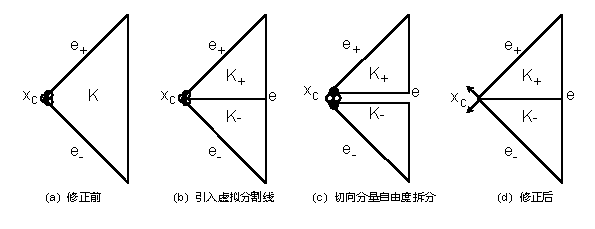
\includegraphics[width=0.70\linewidth]{vertex_relaxation.pdf}
			
			\vspace{-0.65em}
			
			{\fontsize{7.2}{9.0}\selectfont\sffamily\bfseries
				复杂边界角点处顶点应力连续性的部分松弛示意}
		\end{center}
		
		\begin{tcolorbox}[
			colback=structure.fg, colframe=structure.fg,
			coltext=white, boxrule=0pt, arc=3pt,
			top=4pt, bottom=4pt, left=8pt, right=8pt]
			{\fontsize{7.5}{11}\selectfont\sffamily
				\setlength{\parskip}{0pt}
				\textbf{\circnum{1} 局部拆分：}松弛角点 $x_c$ 处切向应力分量自由度，分别适配 $K^+$ 与 $K^-$ 两侧边界条件。
				
				\textbf{\circnum{2} 协调保持：}与法向迹相关的自由度仍保持单值，不破坏全局 $H(\operatorname{div})$ 协调性。
				
				\textbf{\circnum{3} 作用机制：}在保持法向迹连续的前提下，解除复杂边界角点处的局部过约束。
			}
		\end{tcolorbox}
		
	\end{frame}
	
	% ============================================================
	%  05-5  低阶胡张混合元的稳定化扩展
	% ============================================================
	
	\begin{frame}
		\frametitle{低阶胡张混合元的稳定化扩展}
		
		\begin{tcolorbox}[
			colback=structure.fg!8, colframe=structure.fg!40,
			arc=2pt, boxrule=0.4pt,
			top=2pt, bottom=2pt, left=8pt, right=8pt]
			{\fontsize{7.8}{10.5}\selectfont\sffamily
				标准 Hu--Zhang 混合格式主要适用于高阶情形；
				为降低拓扑优化迭代中的状态求解规模，
				需要通过跳量稳定化将方法拓展到低阶情形。}
		\end{tcolorbox}
		
		% ============================================================
		% Overlay 1：为什么需要低阶稳定化
		% ============================================================
		\only<1>{
			\begin{tcolorbox}[
				colback=white, colframe=structure.fg!50,
				colbacktitle=structure.fg, coltitle=white,
				fonttitle=\fontsize{8}{10}\selectfont\bfseries\sffamily,
				title={\circnum{01}\enspace 低阶化动机与稳定性限制},
				arc=3pt, boxrule=0.5pt,
				toptitle=3pt, bottomtitle=3pt,
				top=7pt, bottom=7pt, left=12pt, right=12pt,
				height=0.47\paperheight, valign=center]
				{\fontsize{7.45}{10.2}\selectfont\sffamily
					\begin{columns}[T, totalwidth=\linewidth]
						
						\begin{column}{0.48\linewidth}
							\centering
							{\bfseries 高阶标准格式}
							
							\vspace{-2.2em}
							
							\[
							k\ge d+1
							\]
							
							\vspace{-0.5em}
							
							{\fontsize{7.25}{9.6}\selectfont
								满足离散 inf-sup 条件，\\
								可直接使用标准 Hu--Zhang 混合格式。}
							
							\vspace{0.5em}
							
							{\fontsize{7.25}{9.6}\selectfont
								但应力空间阶次较高，\\
								状态方程求解规模相对较大。}
						\end{column}
						
						\begin{column}{0.48\linewidth}
							\centering
							{\bfseries 低阶高效格式}
							
							\vspace{-2.2em}
							
							\[
							1\le k\le d
							\]
							
							\vspace{-0.5em}
							
							{\fontsize{7.25}{9.6}\selectfont
								自由度规模更小，\\
								更适合嵌入拓扑优化迭代。}
							
							\vspace{0.5em}
							
							{\fontsize{7.25}{9.6}\selectfont
								但 $\operatorname{div}\boldsymbol{\Sigma}_h^k$
								与 $\boldsymbol{V}_h^{k-1}$ 相容性不足，\\
								需通过稳定化恢复离散 inf-sup 稳定性。}
						\end{column}
						
					\end{columns}
					
					\vspace{0.3em}
					
					\[
					\text{高阶稳定但代价较高}
					\quad\Longrightarrow\quad
					\text{低阶高效但需稳定化}
					\]
				}
			\end{tcolorbox}
			
			\begin{tcolorbox}[
				colback=structure.fg, colframe=structure.fg,
				coltext=white, boxrule=0pt, arc=3pt,
				top=2pt, bottom=2pt, left=8pt, right=8pt]
				{\fontsize{7.2}{9.6}\selectfont\sffamily
					\setlength{\parskip}{0pt}
					\textbf{\circnum{1} 低阶动机：}降低状态求解规模，适配拓扑优化迭代。\\[-2pt]
					\textbf{\circnum{2} 核心障碍：}低阶区间需通过稳定化恢复离散 inf-sup 稳定性。
				}
			\end{tcolorbox}
		}
		
		% ============================================================
		% Overlay 2：矩阵型跳量稳定化格式
		% ============================================================
		\only<2>{
			\begin{tcolorbox}[
				colback=white, colframe=structure.fg!50,
				colbacktitle=structure.fg, coltitle=white,
				fonttitle=\fontsize{8}{10}\selectfont\bfseries\sffamily,
				title={\circnum{02}\enspace 矩阵型跳量稳定化格式},
				arc=3pt, boxrule=0.5pt,
				toptitle=3pt, bottomtitle=3pt,
				top=5pt, bottom=5pt, left=12pt, right=12pt]
				{\fontsize{7.15}{9.4}\selectfont\sffamily
					
					\centering
					{\bfseries 矩阵型跳量稳定化项}
					
					\vspace{-2.0em}
					
					\[
					c_{\mathrm{mat}}(\boldsymbol{u}_h,\boldsymbol{v}_h)
					:=
					\sum_{F\in\mathcal{F}_h}
					h_F\int_F
					[\![\boldsymbol{u}_h]\!]:
					[\![\boldsymbol{v}_h]\!]\,\mathrm{d}s,
					\qquad
					\mathcal{F}_h=\mathcal{F}_h^{i}\cup\mathcal{F}_h^{D}.
					\]
					
					\vspace{-1.0em}
					
					{\fontsize{7.0}{9.2}\selectfont
						其中 $[\![\cdot]\!]$ 为法向耦合的矩阵型位移跳量；
						稳定化项仅作用于内部面与位移边界面，不作用于牵引边界。}
					
					\vspace{0.15em}
					
					\begin{columns}[T, totalwidth=\linewidth]
						
						\begin{column}{0.43\linewidth}
							\centering
							{\bfseries 阶次处理}
							
							\vspace{-2.5em}
							
							\[
							\begin{cases}
								k\ge d+1, & c_{\mathrm{mat}}=0,\\[1pt]
								1\le k\le d, & c_{\mathrm{mat}}\ne 0.
							\end{cases}
							\]

						\end{column}
						
						\begin{column}{0.53\linewidth}
							\centering
							{\bfseries 稳定化后的混合格式}
							
							\vspace{-2.5em}
							
							\[
							\left\{
							\begin{aligned}
								a(\boldsymbol{\sigma}_h,\boldsymbol{\tau}_h)
								+
								b(\boldsymbol{\tau}_h,\boldsymbol{u}_h)
								&=
								\ell(\boldsymbol{\tau}_h),
								\\
								b(\boldsymbol{\sigma}_h,\boldsymbol{v}_h)
								-
								c_{\mathrm{mat}}(\boldsymbol{u}_h,\boldsymbol{v}_h)
								&=
								f(\boldsymbol{v}_h)
								-
								c_{\mathrm{bdy}}(\boldsymbol{u}_D,\boldsymbol{v}_h).
							\end{aligned}
							\right.
							\]
						\end{column}
						
					\end{columns}
				}
			\end{tcolorbox}
			
			\begin{tcolorbox}[
				colback=structure.fg, colframe=structure.fg,
				coltext=white, boxrule=0pt, arc=3pt,
				top=2pt, bottom=2pt, left=8pt, right=8pt]
				{\fontsize{7.0}{9.2}\selectfont\sffamily
					\textbf{\circnum{1} 稳定机制：}矩阵型跳量项惩罚界面非协调跳跃，恢复低阶离散 inf-sup 稳定性。\\[-2pt]
					\textbf{\circnum{2} 边界补偿：}$c_{\mathrm{bdy}}(\boldsymbol{u}_D,\boldsymbol{v}_h)$ 表示非齐次位移边界数据诱导的右端补偿项。
				}
			\end{tcolorbox}
		}
		
	\end{frame}
	
	% ============================================================
	%  05-5  最小柔顺度问题的互补能列式
	% ============================================================
	
	\begin{frame}
		\frametitle{最小柔顺度问题的互补能列式}
		
		% ── 顶部引导语 ─────────────────────────────────────────────
		\begin{tcolorbox}[
			colback=structure.fg!7,
			colframe=structure.fg!35,
			arc=2pt,
			boxrule=0.35pt,
			top=3pt, bottom=3pt, left=8pt, right=8pt]
			{\fontsize{8.0}{11.2}\selectfont\sffamily
				胡张混合有限元将应力作为独立求解变量，
				因此最小柔顺度问题可直接转化为基于互补应变能的应力--柔度型优化模型。}
		\end{tcolorbox}
		
		% ── 中心模型框 ─────────────────────────────────────────────
		\begin{tcolorbox}[
			colback=white,
			colframe=structure.fg!55,
			colbacktitle=structure.fg,
			coltitle=white,
			fonttitle=\fontsize{8.2}{10.2}\selectfont\bfseries\sffamily,
			title={\enspace 应力--柔度型互补能优化模型},
			arc=3pt,
			boxrule=0.5pt,
			toptitle=2.5pt, bottomtitle=2.5pt,
			top=8pt, bottom=8pt, left=14pt, right=14pt,
			height=0.53\paperheight,
			valign=center]
			
			{\fontsize{8.0}{10.2}\selectfont\sffamily
				
				\centering
				{\bfseries
					从位移--刚度型柔顺度
					\(\boldsymbol{U}^{\top}\boldsymbol{K}(\rho)\boldsymbol{U}\)
					转为应力--柔度型互补能
					\(\boldsymbol{\Sigma}^{\top}
					\boldsymbol{A}_{\sigma\sigma}(\rho)
					\boldsymbol{\Sigma}\)}
				
				\vspace{-1.0em}
				
				\begingroup
				\setlength{\jot}{1.5pt}
				\[
				\left\{
				\begin{aligned}
					\min_{\rho}\quad
					& c(\boldsymbol{\Sigma},\rho)
					=
					\boldsymbol{\Sigma}^{\top}
					\boldsymbol{A}_{\sigma\sigma}(\rho)
					\boldsymbol{\Sigma},
					\\[-1pt]
					\mathrm{s.t.}\quad
					&
					\begin{bmatrix}
						\boldsymbol{A}_{\sigma\sigma}(\rho) 
						& \boldsymbol{B}_{\sigma u}\\
						\boldsymbol{B}_{u\sigma} 
						& \boldsymbol{0}
					\end{bmatrix}
					\begin{Bmatrix}
						\boldsymbol{\Sigma}\\
						\boldsymbol{U}
					\end{Bmatrix}
					=
					\begin{Bmatrix}
						\boldsymbol{0}\\
						\boldsymbol{0}
					\end{Bmatrix},
					\\[-1pt]
					&
					g_V(\rho)
					=
					\frac{V(\rho)}{V_0}
					-
					V_f
					\le 0,
					\\[-1pt]
					&
					\rho_e\in[\rho_{\min},1],
					\qquad
					e=1,\ldots,N_c .
				\end{aligned}
				\right.
				\]
				\endgroup
				
				\vspace{-0.65em}
				
				其中 \(\boldsymbol{A}_{\sigma\sigma}(\rho)\) 为柔度矩阵，
				牵引外载荷通过应力边界自由度施加，系统右端为零向量。
			
			}
			
		\end{tcolorbox}
		
		% ── 底部结论条 ───────────────────────────────────────────
		\begin{tcolorbox}[
			colback=structure.fg,
			colframe=structure.fg,
			coltext=white,
			boxrule=0pt,
			arc=3pt,
			top=3pt, bottom=3pt, left=8pt, right=8pt]
			\centering
			{\fontsize{7.6}{10.2}\selectfont\sffamily
				互补能列式使胡张混合元的“原生应力变量”直接进入拓扑优化目标函数。}
		\end{tcolorbox}
		
	\end{frame}
	
	% ============================================================
	%  05-6  近不可压缩材料情形下的插值模型修正
	% ============================================================
	
	\begin{frame}
		\frametitle{近不可压缩材料情形下的插值模型修正}
		
		% ── 顶部引导语 ─────────────────────────────────────────────
		\begin{tcolorbox}[
			colback=structure.fg!7,
			colframe=structure.fg!35,
			arc=2pt,
			boxrule=0.35pt,
			top=3pt, bottom=3pt, left=8pt, right=8pt]
			{\fontsize{8.0}{11.2}\selectfont\sffamily
				近不可压缩材料拓扑优化中，低密度弱材料不应继承实体材料的近不可压缩属性；
				因此需要对 \(E(\rho)\) 与 \(\nu(\rho)\) 进行联合插值。}
		\end{tcolorbox}
		
		\vspace{-1.5em}
		
		% ── 主体双栏 ─────────────────────────────────────────────
		\begin{columns}[T, totalwidth=\linewidth]
			
			% ─── 左栏：问题来源 ─────────────────────────────────
			\begin{column}{0.48\linewidth}
				\begin{tcolorbox}[
					colback=white,
					colframe=structure.fg!55,
					colbacktitle=structure.fg,
					coltitle=white,
					fonttitle=\fontsize{8.2}{10}\selectfont\bfseries\sffamily,
					title={01\quad 问题来源},
					arc=3pt,
					boxrule=0.5pt,
					toptitle=0.3pt,
					bottomtitle=0.3pt,
					top=5pt, bottom=5pt, left=7pt, right=7pt,
					height=0.45\paperheight,
					valign=top]
					
					{\fontsize{8.0}{10.8}\selectfont\sffamily
						
						\vspace{0.5em}
												
						\centering
						{\bfseries 近不可压缩极限}
						
						\vspace{0.5em}
						
						\setbeamertemplate{itemize item}{\raisebox{1pt}{\tiny$\bullet$}}
						\setlength{\leftmargini}{1.0em}
						\begin{itemize}
							\setlength{\itemsep}{5pt}
							\setlength{\topsep}{1pt}
							\setlength{\parsep}{0pt}
							\setlength{\parskip}{0pt}
							\item 实体材料近不可压缩时，位移型有限元易出现体积闭锁；
							\item 若孔洞弱材料仍取 \(\nu_0\approx 0.5\)，会引入非物理静水压力；
							\item 因此低密度区应表现为可压缩弱材料。
						\end{itemize}
						
					}
					
				\end{tcolorbox}
			\end{column}
			
			% ─── 右栏：联合插值策略 ─────────────────────────────
			\begin{column}{0.48\linewidth}
				\begin{tcolorbox}[
					colback=white,
					colframe=structure.fg!55,
					colbacktitle=structure.fg,
					coltitle=white,
					fonttitle=\fontsize{8.2}{10}\selectfont\bfseries\sffamily,
					title={02\quad 联合插值策略},
					arc=3pt,
					boxrule=0.5pt,
					toptitle=0.3pt,
					bottomtitle=0.3pt,
					top=5pt, bottom=5pt, left=9pt, right=9pt,
					height=0.45\paperheight,
					valign=center]
					
					{\fontsize{8.0}{10.8}\selectfont\sffamily
						
						\vspace{-0.5em}
						
						\centering
						{\bfseries \(E(\rho)\) 与 \(\nu(\rho)\) 的密度相关插值}
						
						\vspace{-1.5em}
						
						\[
						\begin{aligned}
							E(\rho_e)
							&=
							E_{\min}
							+
							\rho_e^{p}
							\bigl(E_0-E_{\min}\bigr),
							\\[3pt]
							\nu(\rho_e)
							&=
							\nu_{\mathrm{void}}
							+
							\rho_e^{p_{\nu}}
							\bigl(\nu_0-\nu_{\mathrm{void}}\bigr).
						\end{aligned}
						\]
						
						\vspace{-1.5em}
						
						\[
						\begin{aligned}
							&\rho_e\to0:
							(E,\nu)\to(E_{\min},\nu_{\mathrm{void}}),\\
							&\rho_e\to1:
							(E,\nu)\to(E_0,\nu_0).
						\end{aligned}
						\]
					
					}
					
				\end{tcolorbox}
				
			\end{column}
			
		\end{columns}
		
		\vspace{0.35em}
		
		% ── 底部结论条 ───────────────────────────────────────────
		\begin{tcolorbox}[
			colback=structure.fg,
			colframe=structure.fg,
			coltext=white,
			boxrule=0pt,
			arc=3pt,
			top=3pt, bottom=3pt, left=8pt, right=8pt]
			\centering
			{\fontsize{7.55}{10.1}\selectfont\sffamily
				近不可压缩情形下，互补能优化模型保持不变；
				只需更新
				\(\boldsymbol{A}_{\sigma\sigma}(\rho_e)
				=
				\boldsymbol{A}_{\sigma\sigma}(E(\rho_e),\nu(\rho_e))\)，
				以排除低密度区非物理压力干扰。}
		\end{tcolorbox}
		
	\end{frame}
	
	% ============================================================
	%  05-7  基于独立表观应力的应力约束列式
	% ============================================================
	
	\begin{frame}
		\frametitle{基于独立表观应力的应力约束列式}
		
		% ── 顶部引导语 ─────────────────────────────────────────────
		\begin{tcolorbox}[
			colback=structure.fg!7,
			colframe=structure.fg!35,
			arc=2pt,
			boxrule=0.35pt,
			top=3pt, bottom=3pt, left=8pt, right=8pt]
			{\fontsize{8.0}{11.2}\selectfont\sffamily
				胡张混合元将全局应力场作为原生求解变量；
				因此局部应力约束可直接建立在独立表观应力
				\(\boldsymbol{\Sigma}\) 上，并进一步构造无奇异约束函数。}
		\end{tcolorbox}
		
		\vspace{-0.65em}
		
		% ============================================================
		% Overlay 1：应力约束体积最小化模型
		% ============================================================
		\only<1>{
			\begin{tcolorbox}[
				colback=white,
				colframe=structure.fg!55,
				colbacktitle=structure.fg,
				coltitle=white,
				fonttitle=\fontsize{8.2}{10.2}\selectfont\bfseries\sffamily,
				title={\enspace 应力约束体积最小化模型},
				arc=3pt,
				boxrule=0.5pt,
				toptitle=2.5pt,
				bottomtitle=2.5pt,
				top=7pt, bottom=7pt, left=12pt, right=12pt,
				height=0.52\paperheight,
				valign=center]
				
				{\fontsize{7.85}{10.4}\selectfont\sffamily
					\setlength{\abovedisplayskip}{4pt}
					\setlength{\belowdisplayskip}{4pt}
					\setlength{\abovedisplayshortskip}{3pt}
					\setlength{\belowdisplayshortskip}{3pt}
					
					\noindent
					{\bfseries\color{structure.fg}
						从位移后处理应力约束，转为独立应力自由度约束}
					
					\vspace{-0.80em}
					
					\begingroup
					\setlength{\jot}{2pt}
					\[
					\left\{
					\begin{aligned}
						\min_{\rho}\quad
						&
						f(\rho)
						=
						\frac{V(\rho)}{V_0},
						\\[2pt]
						\mathrm{s.t.}\quad
						&
						\begin{bmatrix}
							\boldsymbol{A}_{\sigma\sigma}(\rho)
							&
							\boldsymbol{B}_{\sigma u}
							\\
							\boldsymbol{B}_{u\sigma}
							&
							\boldsymbol{0}
						\end{bmatrix}
						\begin{Bmatrix}
							\boldsymbol{\Sigma}\\
							\boldsymbol{U}
						\end{Bmatrix}
						=
						\begin{Bmatrix}
							\boldsymbol{0}\\
							\boldsymbol{0}
						\end{Bmatrix},
						\\[3pt]
						&
						g_{\sigma,e}(\boldsymbol{\Sigma})
						=
						\sigma^{\mathrm{vM}}_{e}(\boldsymbol{\Sigma})
						-
						\bar{\sigma}
						\le 0,
						\qquad
						e=1,\ldots,N_e,
						\\[2pt]
						&
						\rho_e\in[\rho_{\min},1],
						\qquad
						e=1,\ldots,N_e .
					\end{aligned}
					\right.
					\]
					\endgroup
					
					{\fontsize{7.15}{9.5}\selectfont
						其中 \(\sigma^{\mathrm{vM}}_e(\boldsymbol{\Sigma})\)
						由胡张混合元原生求解的独立应力场提取。}
				}
			\end{tcolorbox}
			
			\begin{tcolorbox}[
				colback=structure.fg,
				colframe=structure.fg,
				coltext=white,
				boxrule=0pt,
				arc=3pt,
				top=3pt, bottom=3pt, left=8pt, right=8pt]
				\centering
				{\fontsize{7.55}{10.1}\selectfont\sffamily
					局部应力约束由位移场
					\(\boldsymbol{U}\) 的后处理应力，
					转为直接依赖胡张混合元的独立应力自由度
					\(\boldsymbol{\Sigma}\)。}
			\end{tcolorbox}
		}
		
		% ============================================================
		% Overlay 2：基于独立表观应力的无奇异约束
		% ============================================================
		\only<2>{
			\begin{columns}[T, totalwidth=\linewidth]
				
				% ─── 左栏：表观应力含义 ─────────────────────────────
				\begin{column}{0.485\linewidth}
					\begin{tcolorbox}[
						colback=white,
						colframe=structure.fg!55,
						colbacktitle=structure.fg,
						coltitle=white,
						fonttitle=\fontsize{8.2}{10}\selectfont\bfseries\sffamily,
						title={01\quad 表观应力的物理含义},
						arc=3pt,
						boxrule=0.5pt,
						toptitle=0.3pt,
						bottomtitle=0.3pt,
						top=6pt, bottom=6pt, left=9pt, right=9pt,
						height=0.47\paperheight,
						valign=center]
						
						{\fontsize{7.8}{10.5}\selectfont\sffamily
							
							\centering
							{\bfseries 表观应力与实体应力的关系}
							
							\vspace{-0.8em}
							
							\[
							\boldsymbol{\Sigma}
							\approx
							m_E(\rho)\,
							\boldsymbol{\sigma}_0 .
							\]
							
							\vspace{-0.3em}
							
							\raggedright
							\setbeamertemplate{itemize item}{\raisebox{1pt}{\tiny$\bullet$}}
							\setlength{\leftmargini}{1.0em}
							\begin{itemize}
								\setlength{\itemsep}{4pt}
								\setlength{\topsep}{1pt}
								\setlength{\parsep}{0pt}
								\setlength{\parskip}{0pt}
								\item \(\boldsymbol{\Sigma}\) 是混合元原生求解的宏观表观应力；
								\item \(\boldsymbol{\sigma}_0\) 表示材料内部真实实体应力；
								\item 当 \(\rho_e\to0\) 时，\(\boldsymbol{\Sigma}\to\boldsymbol{0}\)，
								直接校核会误判低密度区“绝对安全”。
							\end{itemize}
						}
					\end{tcolorbox}
				\end{column}
				
				% ─── 右栏：无奇异约束函数 ─────────────────────────
				\begin{column}{0.485\linewidth}
					\begin{tcolorbox}[
						colback=white,
						colframe=structure.fg!55,
						colbacktitle=structure.fg,
						coltitle=white,
						fonttitle=\fontsize{8.2}{10}\selectfont\bfseries\sffamily,
						title={02\quad 无奇异约束函数},
						arc=3pt,
						boxrule=0.5pt,
						toptitle=0.3pt,
						bottomtitle=0.3pt,
						top=6pt, bottom=6pt, left=9pt, right=9pt,
						height=0.47\paperheight,
						valign=center]
						
						{\fontsize{7.75}{10.2}\selectfont\sffamily
							\setlength{\abovedisplayskip}{4pt}
							\setlength{\belowdisplayskip}{4pt}
							
							\centering
							{\bfseries 基于表观应力的归一化约束}
							
							\vspace{-0.9em}
							
							\[
							g_e(\rho,\boldsymbol{\Sigma})
							=
							\frac{
								\sigma^{\mathrm{vM}}_e(\boldsymbol{\Sigma})
							}{\bar{\sigma}}
							-
							\eta(\rho_e)
							\le 0 .
							\]
							
							\vspace{-0.9em}
							
							\[
							\eta(\rho_e)
							=
							m_E(\rho_e)
							+
							\varepsilon
							\bigl(1-m_E(\rho_e)\bigr).
							\]
							
							\vspace{-0.5em}
							
							\[
							\begin{array}{ll}
								\rho_e\to0:
								&
								\eta(\rho_e)\to\varepsilon,\quad
								g_e\to-\varepsilon\le0,
								\\[2pt]
								\rho_e\approx1:
								&
								\eta(\rho_e)\approx1,\quad
								\sigma^{\mathrm{vM}}_e(\boldsymbol{\Sigma})
								\le\bar{\sigma}.
							\end{array}
							\]
							
							{\fontsize{7.2}{10.2}\selectfont
								约束中不含密度分母，避免低密度应力奇异。}
						}
					\end{tcolorbox}
				\end{column}
				
			\end{columns}
			
%			\vspace{0.30em}
			
			% ── 底部结论条 ───────────────────────────────────────────
			\begin{tcolorbox}[
				colback=structure.fg,
				colframe=structure.fg,
				coltext=white,
				boxrule=0pt,
				arc=3pt,
				top=3pt, bottom=3pt, left=8pt, right=8pt]
				\centering
				{\fontsize{7.45}{10.0}\selectfont\sffamily
					第四章通过消失约束处理位移法后处理应力；
					本章基于原生表观应力
					\(\boldsymbol{\Sigma}\)
					重构阈值函数
					\(\eta(\rho_e)\)。}
			\end{tcolorbox}
		}
		
	\end{frame}
	
	% ============================================================
	%  05-8  最小柔顺度基准算例：两端固支梁
	% ============================================================
	
	\begin{frame}
		\frametitle{最小柔顺度基准算例：两端固支梁}
		
		% ── 顶部引导语 ─────────────────────────────────────────────
		\begin{tcolorbox}[
			colback=structure.fg!8,
			colframe=structure.fg!40,
			arc=2pt,
			boxrule=0.4pt,
			top=3pt, bottom=3pt, left=8pt, right=8pt]
			{\fontsize{8}{11}\selectfont\sffamily
				以两端固支梁为基准算例，对比标准位移法与胡张混合法，
				验证混合元拓扑优化闭环的正确性与稳定性。}
		\end{tcolorbox}
		
		\vspace{-0.45em}
		
		% ============================================================
		% Overlay 1：算例设置
		% ============================================================
		\only<1>{
			\begin{tcolorbox}[
				colback=white,
				colframe=structure.fg!55,
				colbacktitle=structure.fg,
				coltitle=white,
				fonttitle=\fontsize{8.4}{10.4}\selectfont\bfseries\sffamily,
				title={\enspace 算例设置},
				arc=3pt,
				boxrule=0.5pt,
				toptitle=2.5pt,
				bottomtitle=2.5pt,
				top=6pt,
				bottom=6pt,
				left=13pt,
				right=13pt,
				height=0.55\paperheight,
				valign=top]
				
				\centering
				
				\vspace{0.75em}
				
				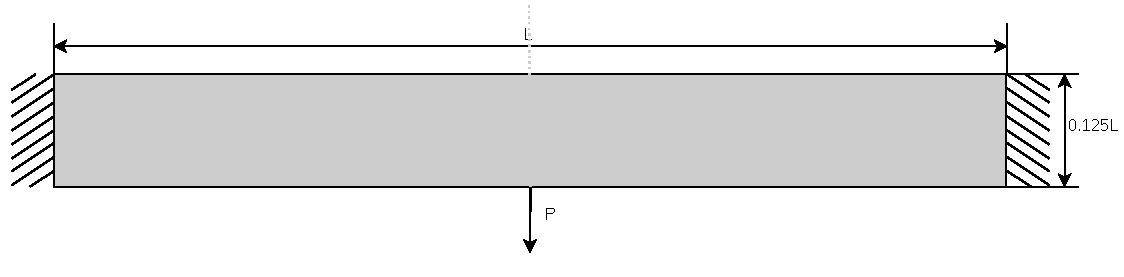
\includegraphics[
				width=0.80\linewidth,
				height=0.255\paperheight,
				keepaspectratio]{fixed_beam_setup}
				
				\vspace{0.75em}
				
				{\fontsize{7.8}{10.6}\selectfont\sffamily
					\setbeamertemplate{itemize item}{\raisebox{1pt}{\tiny$\bullet$}}
					\setlength{\leftmargini}{1.2em}
					
					\begin{minipage}{0.88\linewidth}
						\begin{itemize}
							\setlength{\itemsep}{3pt}
							\setlength{\topsep}{0pt}
							\setlength{\parsep}{0pt}
							\setlength{\parskip}{0pt}
							
							\item 几何尺寸为
							\(\Omega=L\times 0.125L\)；取
							\(L=160\,\mathrm{mm}\)，
							\(E=30\,\mathrm{MPa}\)，
							\(\nu=0.4\)，
							\(V_f=0.4\)。
							
							\item 左右两端完全固支；下边界中点施加竖向集中载荷
							\(P=3\,\mathrm{N}\)。
						\end{itemize}
					\end{minipage}
				}
				
			\end{tcolorbox}
	
		}
		
		% ============================================================
		% Overlay 2：优化结果与构型一致性
		% ============================================================
		\only<2>{
			% ── 列标题行 ─────────────────────────────────────────────
			\begin{columns}[T, totalwidth=\linewidth]
				\begin{column}{0.48\linewidth}\centering
					{\fontsize{8.8}{10.5}\selectfont\sffamily\bfseries\color{structure.fg}
						标准位移法\par}
				\end{column}
				
				\begin{column}{0.48\linewidth}\centering
					{\fontsize{8.8}{10.5}\selectfont\sffamily\bfseries\color{structure.fg}
						胡张混合法\par}
				\end{column}
			\end{columns}
			
			\vspace{0.25em}
			
			% ── 第一行：k = 2 ───────────────────────────────────────
			\begin{columns}[c, totalwidth=\linewidth]
				\begin{column}{0.48\linewidth}\centering
					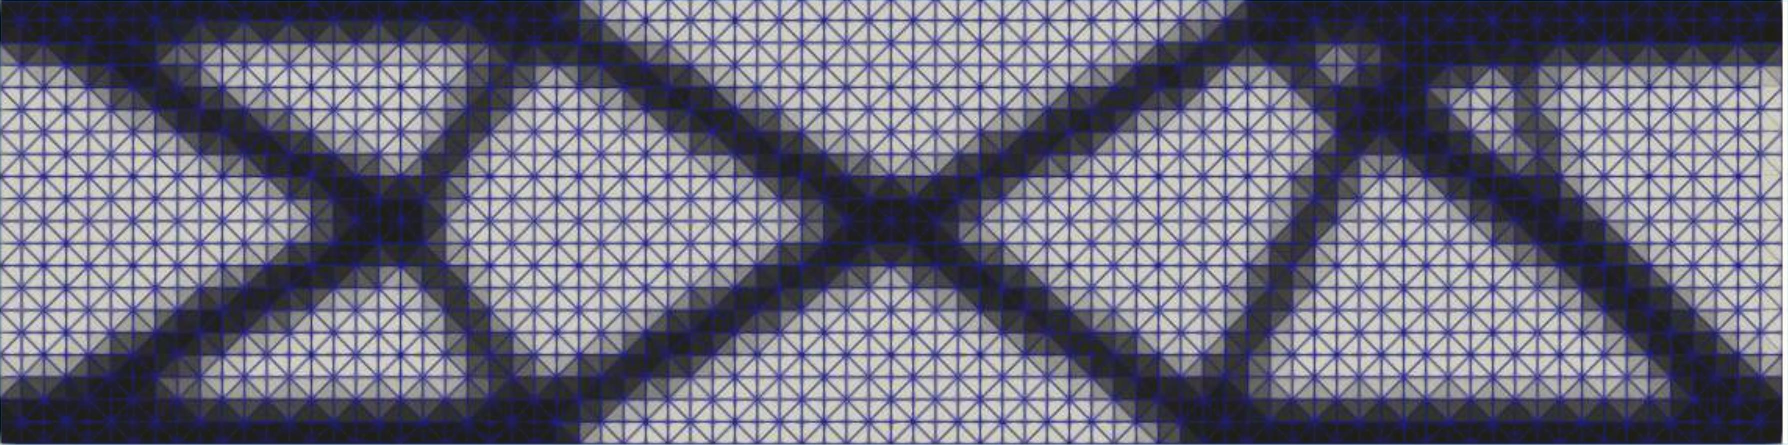
\includegraphics[
					width=0.97\linewidth,
					height=0.195\paperheight,
					keepaspectratio]{fixed_beam_disp_k2}
					
					\vspace{0.10em}
					
					{\fontsize{7.0}{8.8}\selectfont\sffamily
						\(k=2\)：交叉承载路径清晰}
				\end{column}
				
				\begin{column}{0.48\linewidth}\centering
					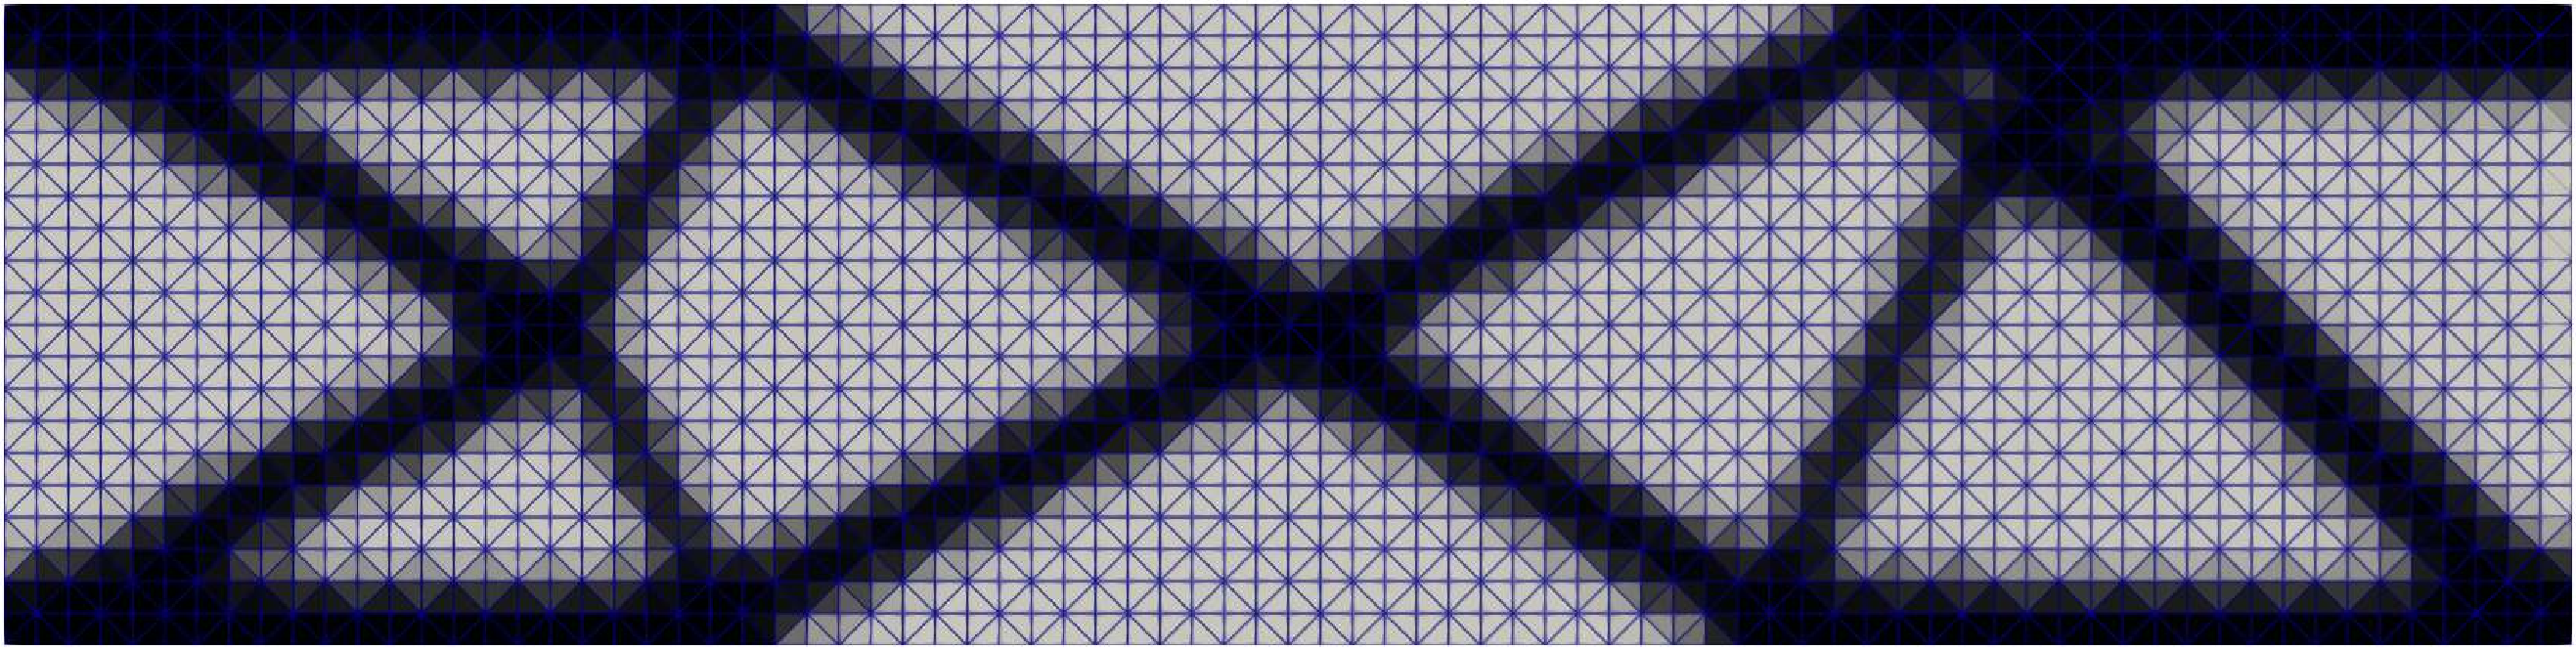
\includegraphics[
					width=0.97\linewidth,
					height=0.195\paperheight,
					keepaspectratio]{fixed_beam_mixed_k2}
					
					\vspace{0.10em}
					
					{\fontsize{7.0}{8.8}\selectfont\sffamily
						\(k=2\)：主拓扑特征保持一致}
				\end{column}
			\end{columns}
			
			\vspace{0.45em}
			
			% ── 第二行：k = 4 ───────────────────────────────────────
			\begin{columns}[c, totalwidth=\linewidth]
				\begin{column}{0.48\linewidth}\centering
					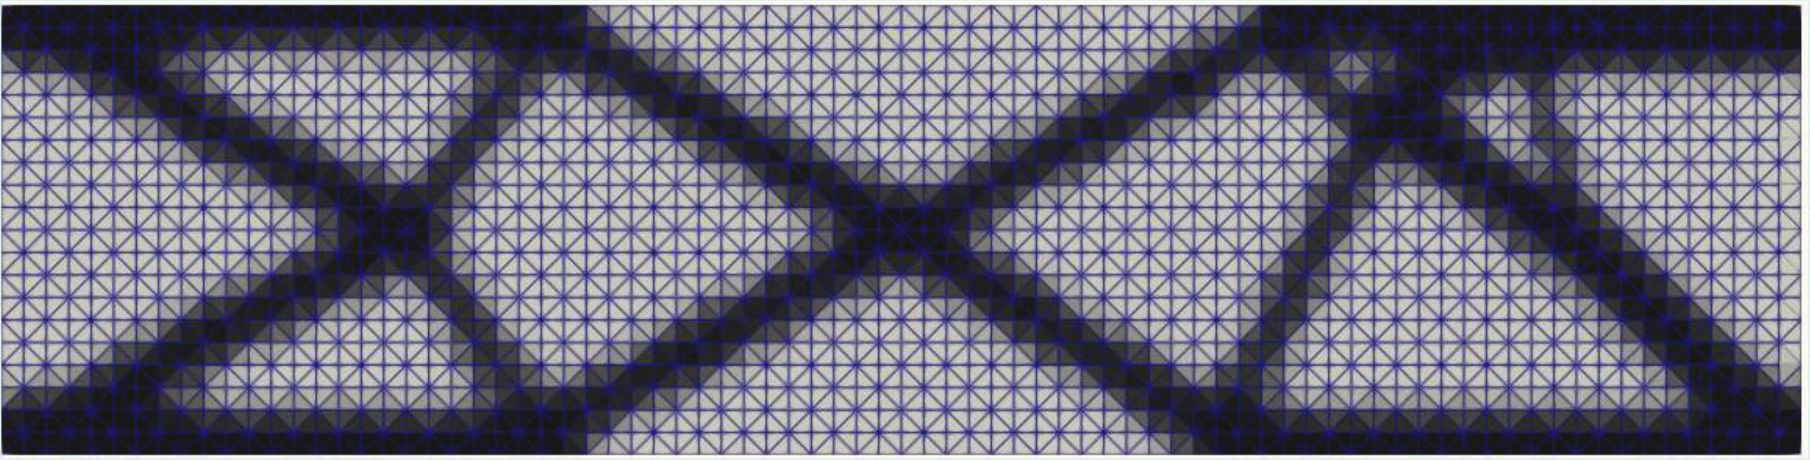
\includegraphics[
					width=0.97\linewidth,
					height=0.195\paperheight,
					keepaspectratio]{fixed_beam_disp_k4}
					
					\vspace{0.10em}
					
					{\fontsize{7.0}{8.8}\selectfont\sffamily
						\(k=4\)：高阶下构型稳定}
				\end{column}
				
				\begin{column}{0.48\linewidth}\centering
					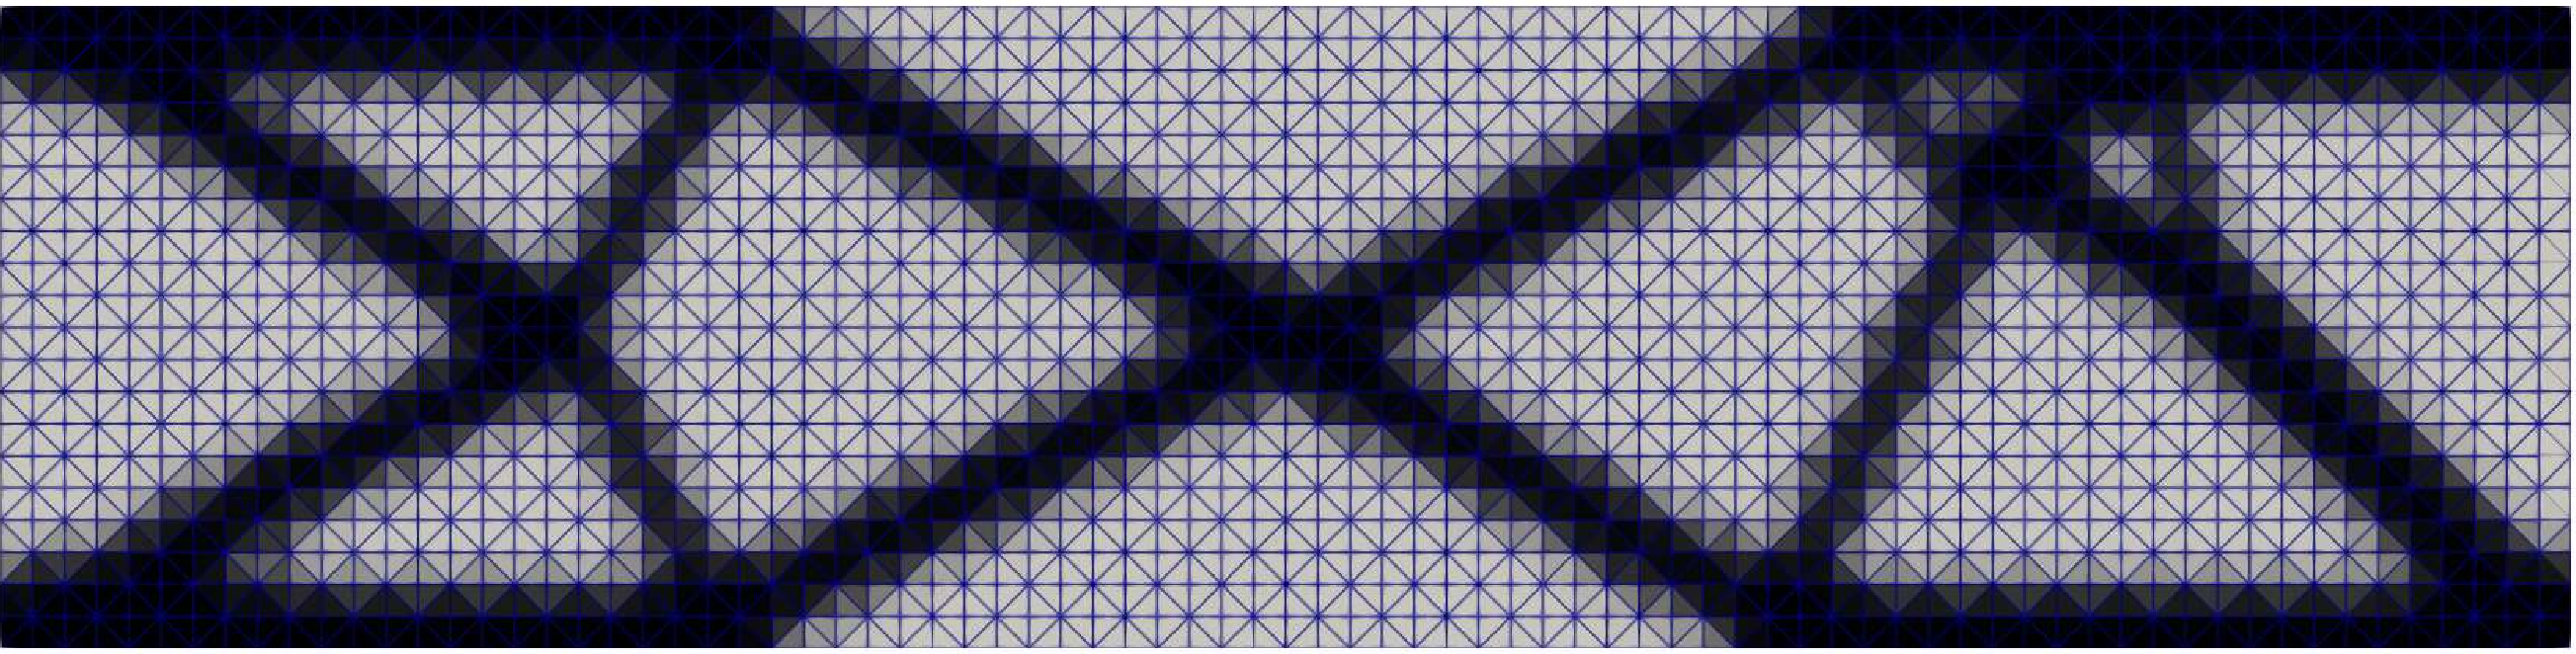
\includegraphics[
					width=0.97\linewidth,
					height=0.195\paperheight,
					keepaspectratio]{fixed_beam_mixed_k4}
					
					\vspace{0.10em}
					
					{\fontsize{7.0}{8.8}\selectfont\sffamily
						\(k=4\)：与位移法结果物理一致}
				\end{column}
			\end{columns}
			
			\vspace{0.35em}
			
			% ── 底部结论：统一蓝色样式 ───────────────────────────────
			\begin{tcolorbox}[
				colback=structure.fg,
				colframe=structure.fg,
				coltext=white,
				boxrule=0pt,
				arc=3pt,
				top=3pt,
				bottom=3pt,
				left=8pt,
				right=8pt]
				\centering
				{\fontsize{7.45}{10.0}\selectfont\sffamily
					胡张混合法与标准位移法均获得物理一致的交叉承载构型，
					说明胡张混合有限元可稳定嵌入柔顺度最小化拓扑优化闭环。}
			\end{tcolorbox}
		}
		
	\end{frame}
	
	% ============================================================
	%  05-9  近不可压缩材料下的抗闭锁能力
	% ============================================================
	
	\begin{frame}
		\frametitle{近不可压缩材料下的抗闭锁能力}
	
		% ============================================================
		% Overlay 1：算例设置
		% ============================================================
		
		\only<1>{		
			\begin{tcolorbox}[
				colback=structure.fg!8,
				colframe=structure.fg!40,
				arc=2pt,
				boxrule=0.4pt,
				top=3pt,
				bottom=3pt,
				left=8pt,
				right=8pt]
				{\fontsize{8}{11}\selectfont\sffamily
					以二维轴承装置为例，在统一几何、载荷与优化参数下仅改变实体材料泊松比，
					检验胡张混合有限元在近不可压缩极限下的抗闭锁能力。}
			\end{tcolorbox}
			
			\vspace{-0.25em}
			
			\begin{tcolorbox}[
				colback=white,
				colframe=structure.fg!55,
				colbacktitle=structure.fg,
				coltitle=white,
				fonttitle=\fontsize{8.4}{10.4}\selectfont\bfseries\sffamily,
				title={算例设置：二维轴承装置},
				arc=3pt,
				boxrule=0.5pt,
				toptitle=2.5pt,
				bottomtitle=2.5pt,
				top=8pt,
				bottom=8pt,
				left=12pt,
				right=12pt,
				height=0.50\paperheight,
				valign=center]
				
				\begin{columns}[c, totalwidth=\linewidth]
					
					% ─── 左侧：算例示意图 ─────────────────────────────
					\begin{column}{0.57\linewidth}
						\centering
						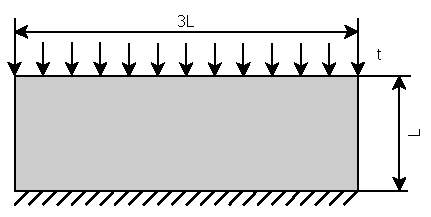
\includegraphics[
						width=0.98\linewidth,
						height=0.34\paperheight,
						keepaspectratio]{bearing_setup}
					\end{column}
					
					% ─── 右侧：基本参数 ───────────────────────────────
					\begin{column}{0.40\linewidth}
						{\fontsize{7.7}{10.5}\selectfont\sffamily
							\setbeamertemplate{itemize item}{\raisebox{1pt}{\tiny$\bullet$}}
							\setlength{\leftmargini}{1.15em}
							
							\begin{itemize}
								\setlength{\itemsep}{8pt}
								\setlength{\topsep}{0pt}
								\setlength{\parsep}{0pt}
								\setlength{\parskip}{0pt}
								
								\item 几何尺寸为 \(3L\times L\)；取 $L=40\,\mathrm{mm}$，$E=1\,\mathrm{MPa}$，$V_f=0.35$;
								
								\item 底部边界完全固支；顶部施加竖向均布牵引 $\boldsymbol{t}=(0,-t_0)^{\mathrm T}$，其中 $t_0=8\times 10^{-2}\,\mathrm{N/mm}$。

							\end{itemize}
						}
					\end{column}
					
				\end{columns}
				
			\end{tcolorbox}

		}
		
		% ============================================================
		% Overlay 2：结果对比
		% ============================================================
		\only<2>{
			% ── 列标题行 ─────────────────────────────────────────────
			\begin{columns}[T, totalwidth=\linewidth]
				\begin{column}{0.10\linewidth}\end{column}
				
				\begin{column}{0.42\linewidth}\centering
					{\fontsize{8.5}{10.2}\selectfont\sffamily\bfseries\color{structure.fg}
						可压缩材料 \enspace \(\nu_0=0.3\)\par}
				\end{column}
				
				\begin{column}{0.42\linewidth}\centering
					{\fontsize{8.5}{10.2}\selectfont\sffamily\bfseries\color{structure.fg}
						近不可压缩材料 \enspace \(\nu_0=0.4999\)\par}
				\end{column}
			\end{columns}
			
			\vspace{0.20em}
			
			% ── 第一行：标准位移法 ─────────────────────────────────
			\begin{columns}[c, totalwidth=\linewidth]
				\begin{column}{0.10\linewidth}\centering
					{\fontsize{8.3}{10.0}\selectfont\sffamily\bfseries\color{structure.fg}
						标准\\[2pt]位移法\\[-1pt]
						{\fontsize{6.5}{8}\selectfont \(k=2\)}}
				\end{column}
				
				\begin{column}{0.42\linewidth}\centering
					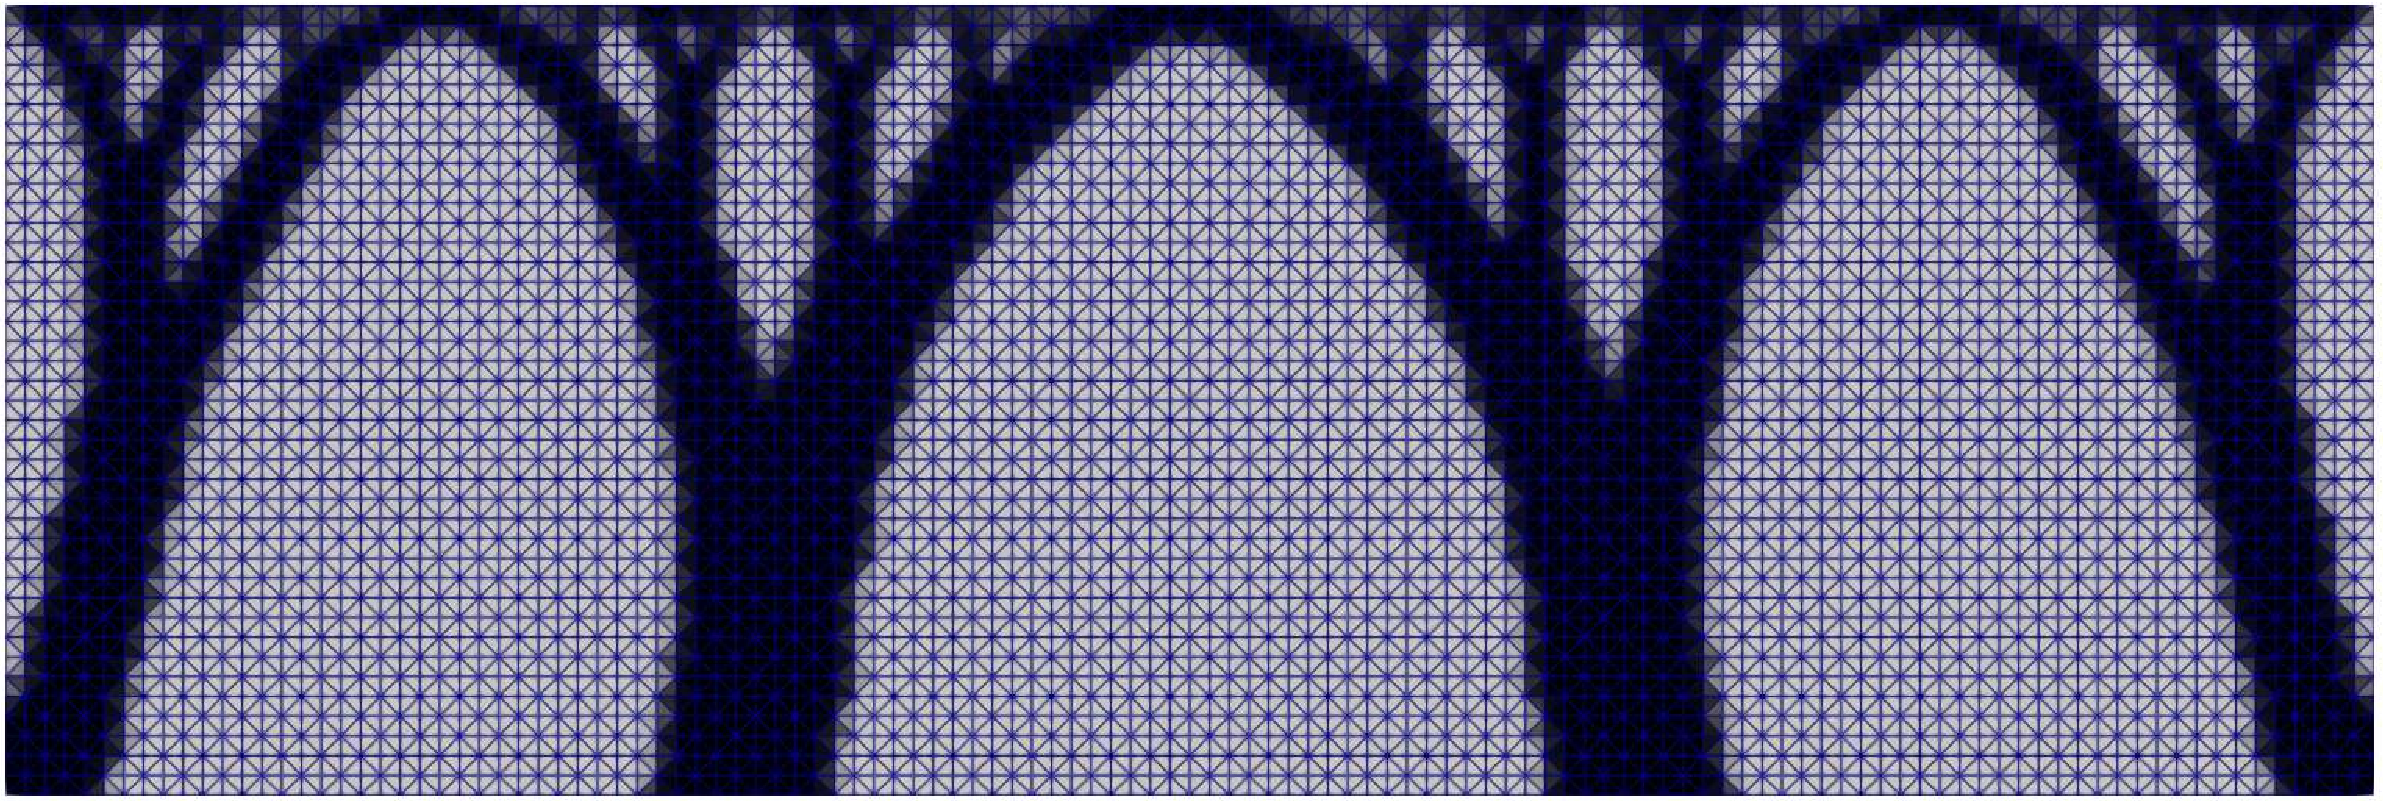
\includegraphics[
					width=0.96\linewidth,
					height=0.19\paperheight,
					keepaspectratio]{bearing_disp_nu03}
					
					\vspace{0.10em}
					
					{\fontsize{7.0}{8.8}\selectfont\sffamily
						\(c=123.3753\)：结构清晰，正常收敛}
				\end{column}
				
				\begin{column}{0.42\linewidth}\centering
					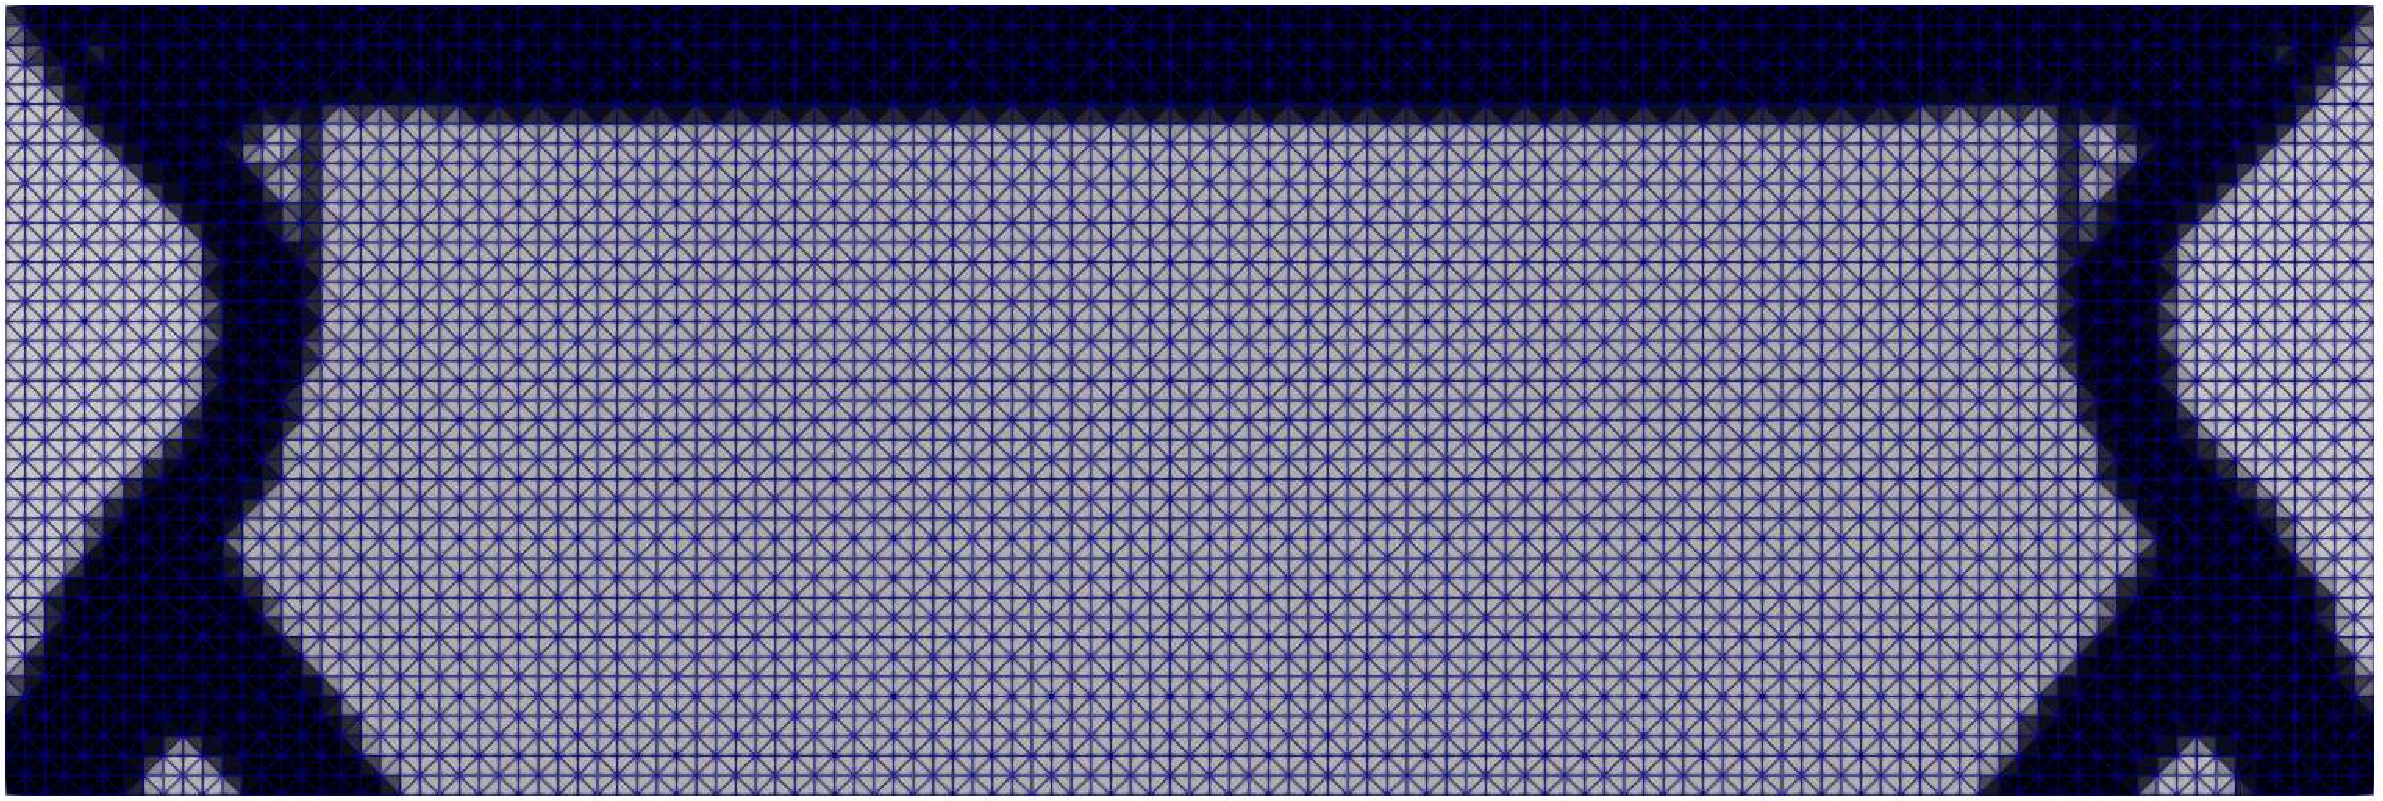
\includegraphics[
					width=0.96\linewidth,
					height=0.19\paperheight,
					keepaspectratio]{bearing_disp_nu4999}
					
					\vspace{0.10em}
					
					{\fontsize{7.0}{8.8}\selectfont\sffamily
						\(c=55.7879\)：刚度高估，构型异常}
				\end{column}
			\end{columns}
			
			\vspace{0.38em}
			
			% ── 第二行：胡张混合法 ─────────────────────────────────
			\begin{columns}[c, totalwidth=\linewidth]
				\begin{column}{0.10\linewidth}\centering
					{\fontsize{8.3}{10.0}\selectfont\sffamily\bfseries\color{structure.fg}
						胡张\\[2pt]混合法\\[-1pt]
						{\fontsize{6.5}{8}\selectfont \(k=2\)}}
				\end{column}
				
				\begin{column}{0.42\linewidth}\centering
					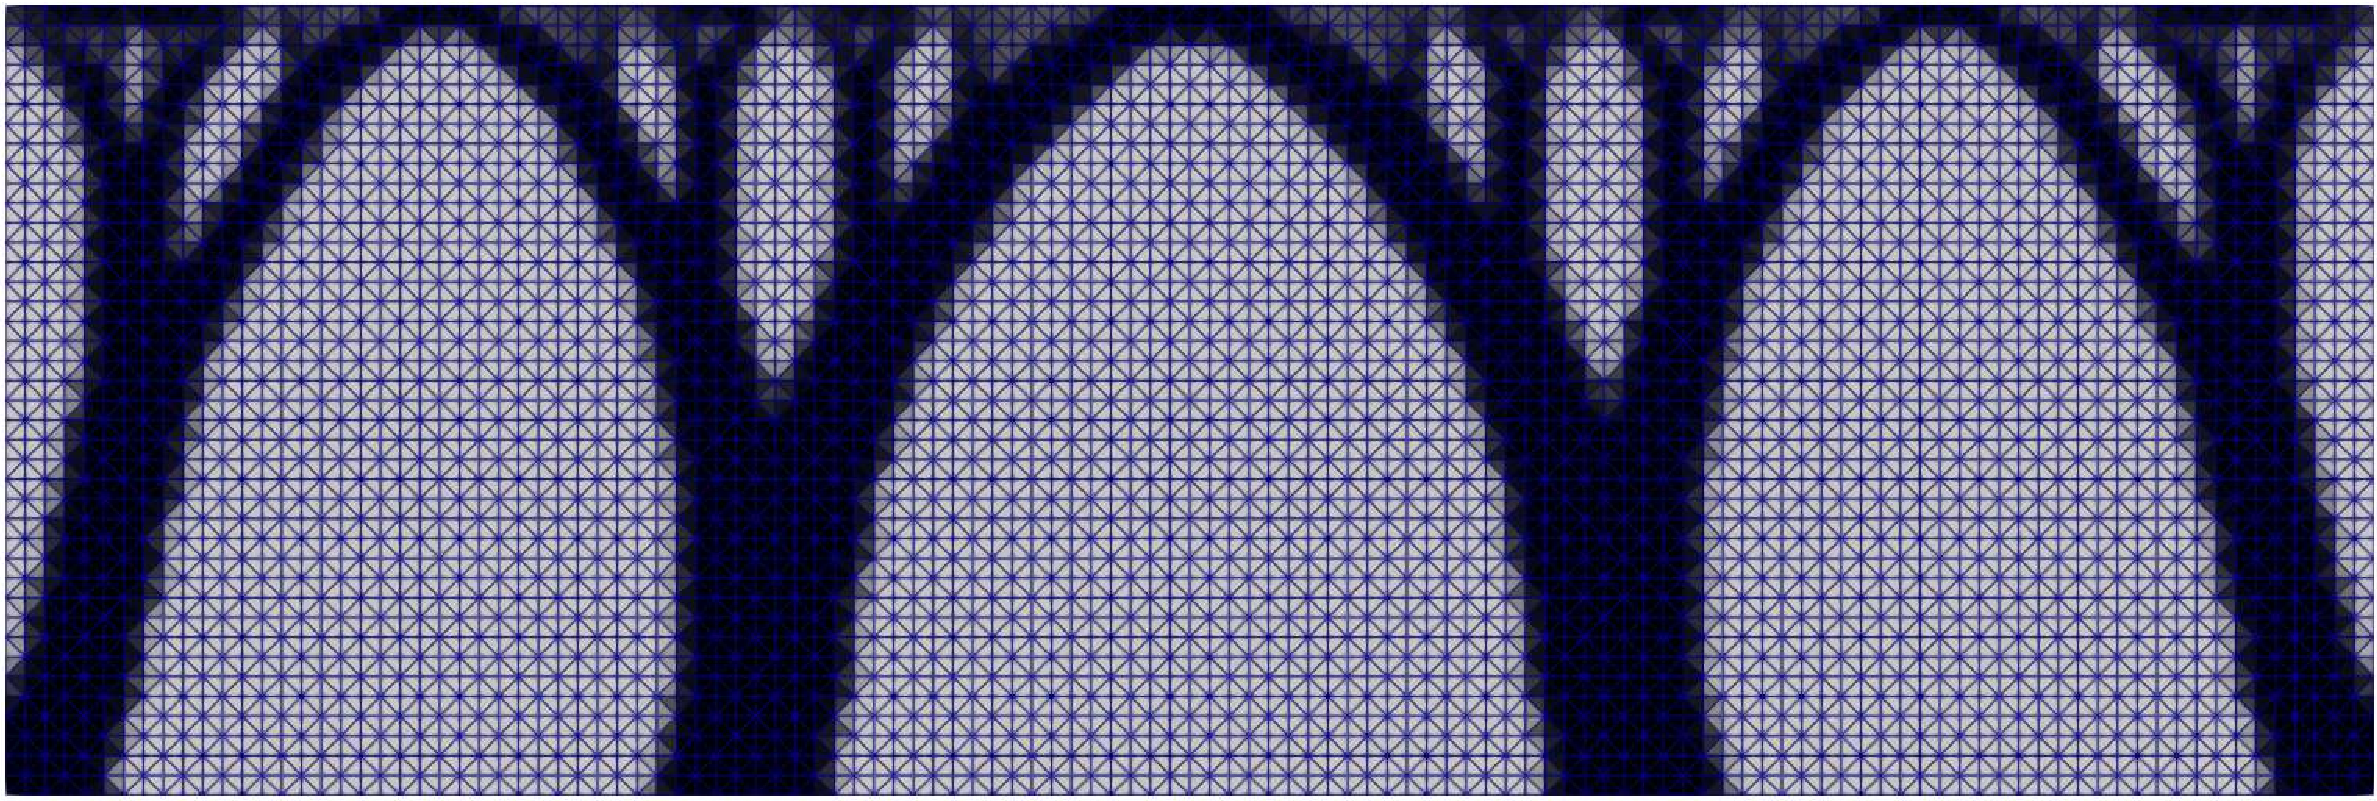
\includegraphics[
					width=0.96\linewidth,
					height=0.19\paperheight,
					keepaspectratio]{bearing_mixed_nu03}
					
					\vspace{0.10em}
					
					{\fontsize{7.0}{8.8}\selectfont\sffamily
						\(c=128.4504\)：结构清晰，结果接近}
				\end{column}
				
				\begin{column}{0.42\linewidth}\centering
					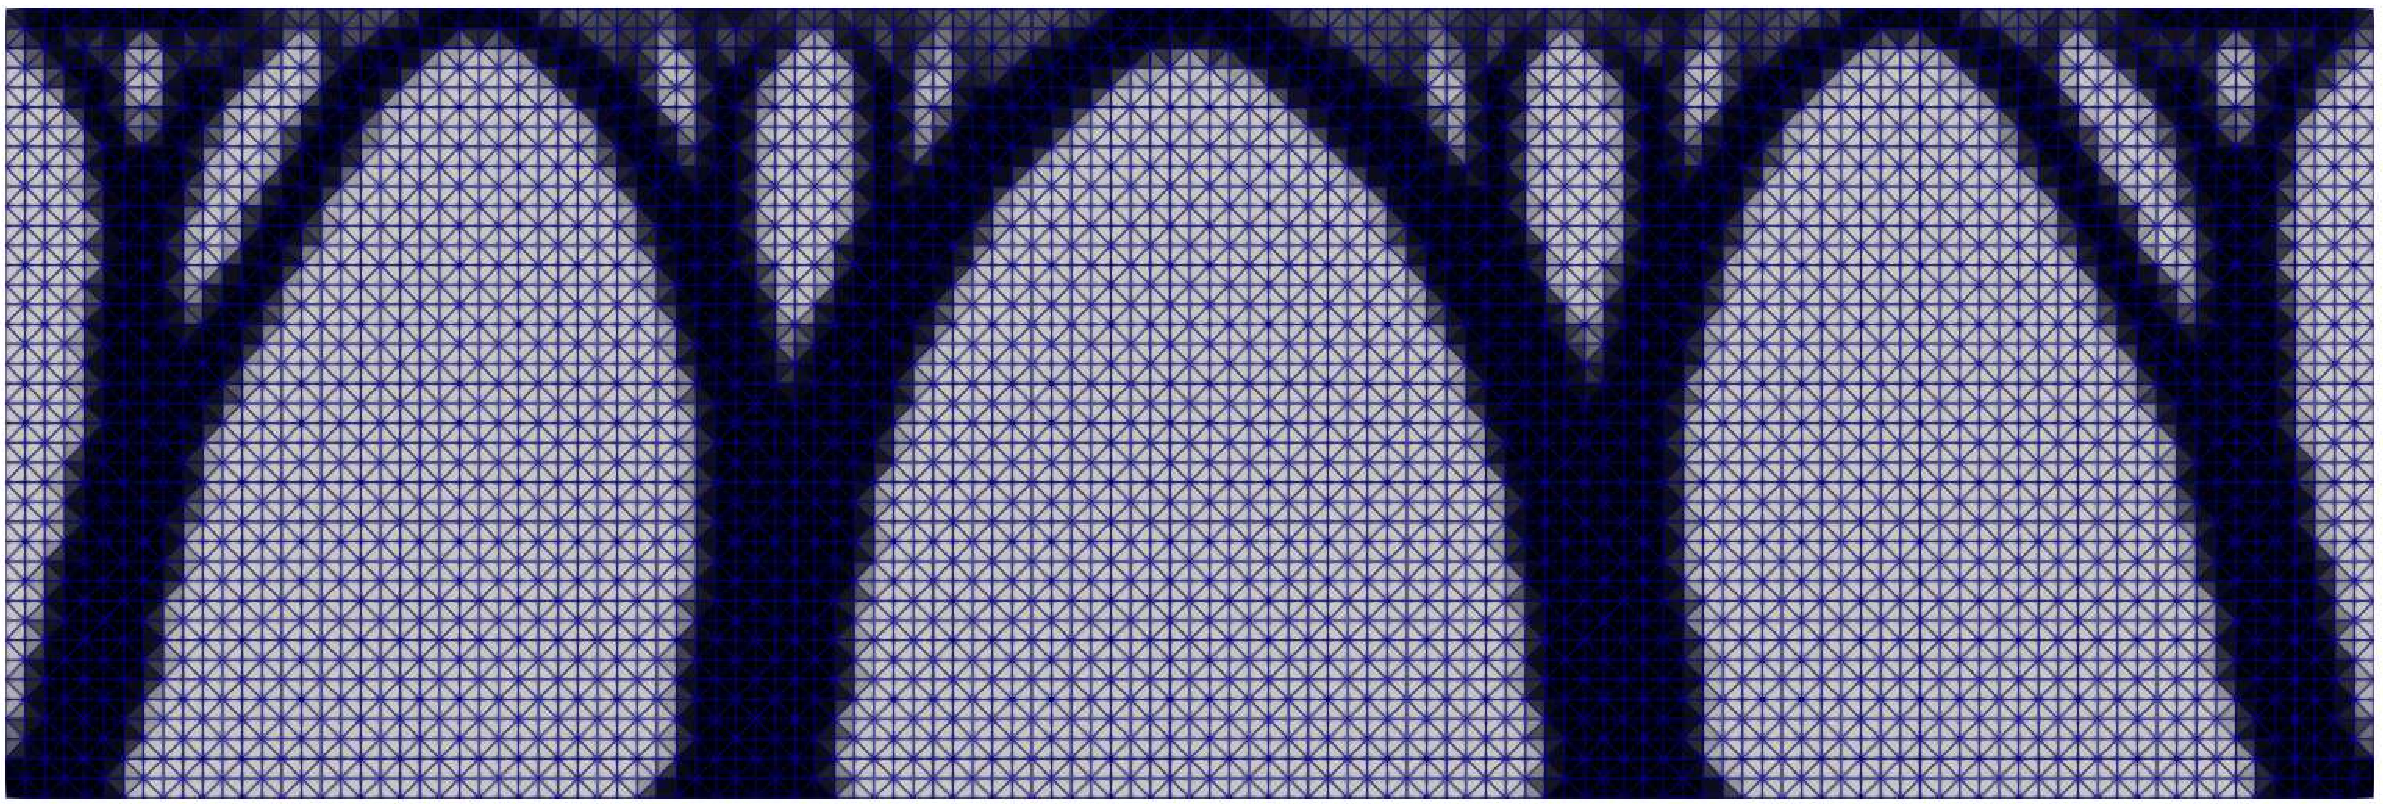
\includegraphics[
					width=0.96\linewidth,
					height=0.19\paperheight,
					keepaspectratio]{bearing_mixed_nu4999}
					
					\vspace{0.10em}
					
					{\fontsize{7.0}{8.8}\selectfont\sffamily
						\(c=102.7948\)：抗体积闭锁，构型稳定}
				\end{column}
			\end{columns}
			
			\vspace{0.32em}
			
			% ── 底部结论条 ───────────────────────────────────────────
			\begin{tcolorbox}[
				colback=structure.fg,
				colframe=structure.fg,
				coltext=white,
				boxrule=0pt,
				arc=3pt,
				top=3pt,
				bottom=3pt,
				left=8pt,
				right=8pt]
				\centering
				{\fontsize{7.45}{10.0}\selectfont\sffamily
					可压缩材料下两类方法均可得到清晰构型；近不可压缩极限下，
					胡张混合有限元有效缓解体积闭锁，避免刚度高估诱发的非物理拓扑演化。}
			\end{tcolorbox}
		}
		
	\end{frame}
	
	% ============================================================
	%  05-10  局部应力约束下的应力场评估能力
	% ============================================================
	
	\begin{frame}
		\frametitle{局部应力约束下的应力场评估能力}
		
		% ============================================================
		% Overlay 1：算例设置
		% ============================================================
		\only<1>{
			% ── 顶部引导语：仅 Overlay 1 使用 ─────────────────────────
			\begin{tcolorbox}[
				colback=structure.fg!8,
				colframe=structure.fg!40,
				arc=2pt,
				boxrule=0.4pt,
				top=3pt,
				bottom=3pt,
				left=8pt,
				right=8pt]
				{\fontsize{8}{11}\selectfont\sffamily
					以端部中点受载的二维悬臂梁为例，对比标准位移法与胡张混合法
					在局部应力约束下的拓扑构型与应力场评估效果。}
			\end{tcolorbox}
			
			\vspace{0.35em}
			
			\begin{tcolorbox}[
				colback=white,
				colframe=structure.fg!55,
				colbacktitle=structure.fg,
				coltitle=white,
				fonttitle=\fontsize{8.4}{10.4}\selectfont\bfseries\sffamily,
				title={算例设置：端部中点受载二维悬臂梁},
				arc=3pt,
				boxrule=0.5pt,
				toptitle=2.5pt,
				bottomtitle=2.5pt,
				top=8pt,
				bottom=8pt,
				left=12pt,
				right=12pt,
				height=0.50\paperheight,
				valign=center]
				
				\begin{columns}[c, totalwidth=\linewidth]
					
					% ─── 左侧：算例示意图 ─────────────────────────────
					\begin{column}{0.55\linewidth}
						\centering
						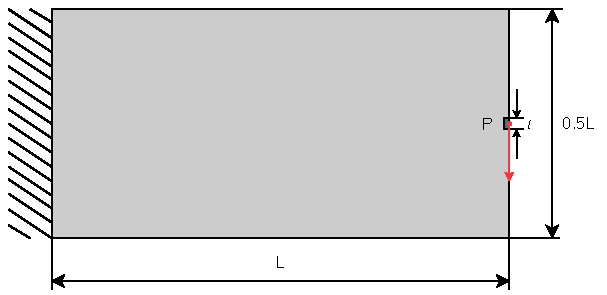
\includegraphics[
						width=0.98\linewidth,
						height=0.34\paperheight,
						keepaspectratio]{stress_cantilever_setup}
					\end{column}
					
					% ─── 右侧：基本参数 ───────────────────────────────
					\begin{column}{0.42\linewidth}
						{\fontsize{7.45}{10.2}\selectfont\sffamily
							\setbeamertemplate{itemize item}{\raisebox{1pt}{\tiny$\bullet$}}
							\setlength{\leftmargini}{1.15em}
							
							\begin{itemize}
								\setlength{\itemsep}{7pt}
								\setlength{\topsep}{0pt}
								\setlength{\parsep}{0pt}
								\setlength{\parskip}{0pt}
								
								\item 几何尺寸为 \(\Omega=L\times 0.5L\)；取
								\(L=80\,\mathrm{mm}\)，
								\(E=70000\,\mathrm{MPa}\)，
								\(\nu=0.25\)，
								\(\bar{\sigma}=180\,\mathrm{MPa}\)。
								
								\item 左侧边缘完全固支；右侧中点施加竖向载荷
								\(P=400\,\mathrm{N}\)，并按长度
								\(l=6\,\mathrm{mm}\) 分布化处理。
							\end{itemize}
						}
					\end{column}
					
				\end{columns}
				
			\end{tcolorbox}
	
		}
		
		% ============================================================
		% Overlay 2：结果对比
		% ============================================================
		\only<2>{
			% ── 列标题行：指标分类 ──────────────────────────────────
			\begin{columns}[T, totalwidth=\linewidth]
				\begin{column}{0.10\linewidth}\end{column}
				
				\begin{column}{0.42\linewidth}\centering
					{\fontsize{9}{11}\selectfont\sffamily\bfseries\color{structure.fg}
						最终拓扑构型\par}
				\end{column}
				
				\begin{column}{0.42\linewidth}\centering
					{\fontsize{9}{11}\selectfont\sffamily\bfseries\color{structure.fg}
						归一化 von Mises 等效应力\par}
				\end{column}
			\end{columns}
			
			\vspace{0.25em}
			
			% ── 第一行：标准位移法 ────────────────────────────────────
			\begin{columns}[c, totalwidth=\linewidth]
				\begin{column}{0.10\linewidth}\centering
					{\fontsize{8.4}{10}\selectfont\sffamily\bfseries\color{structure.fg}
						标准\\[2pt]位移法\\[-1pt]
						{\fontsize{6.5}{8}\selectfont \(k=2\)}}
				\end{column}
				
				\begin{column}{0.42\linewidth}\centering
					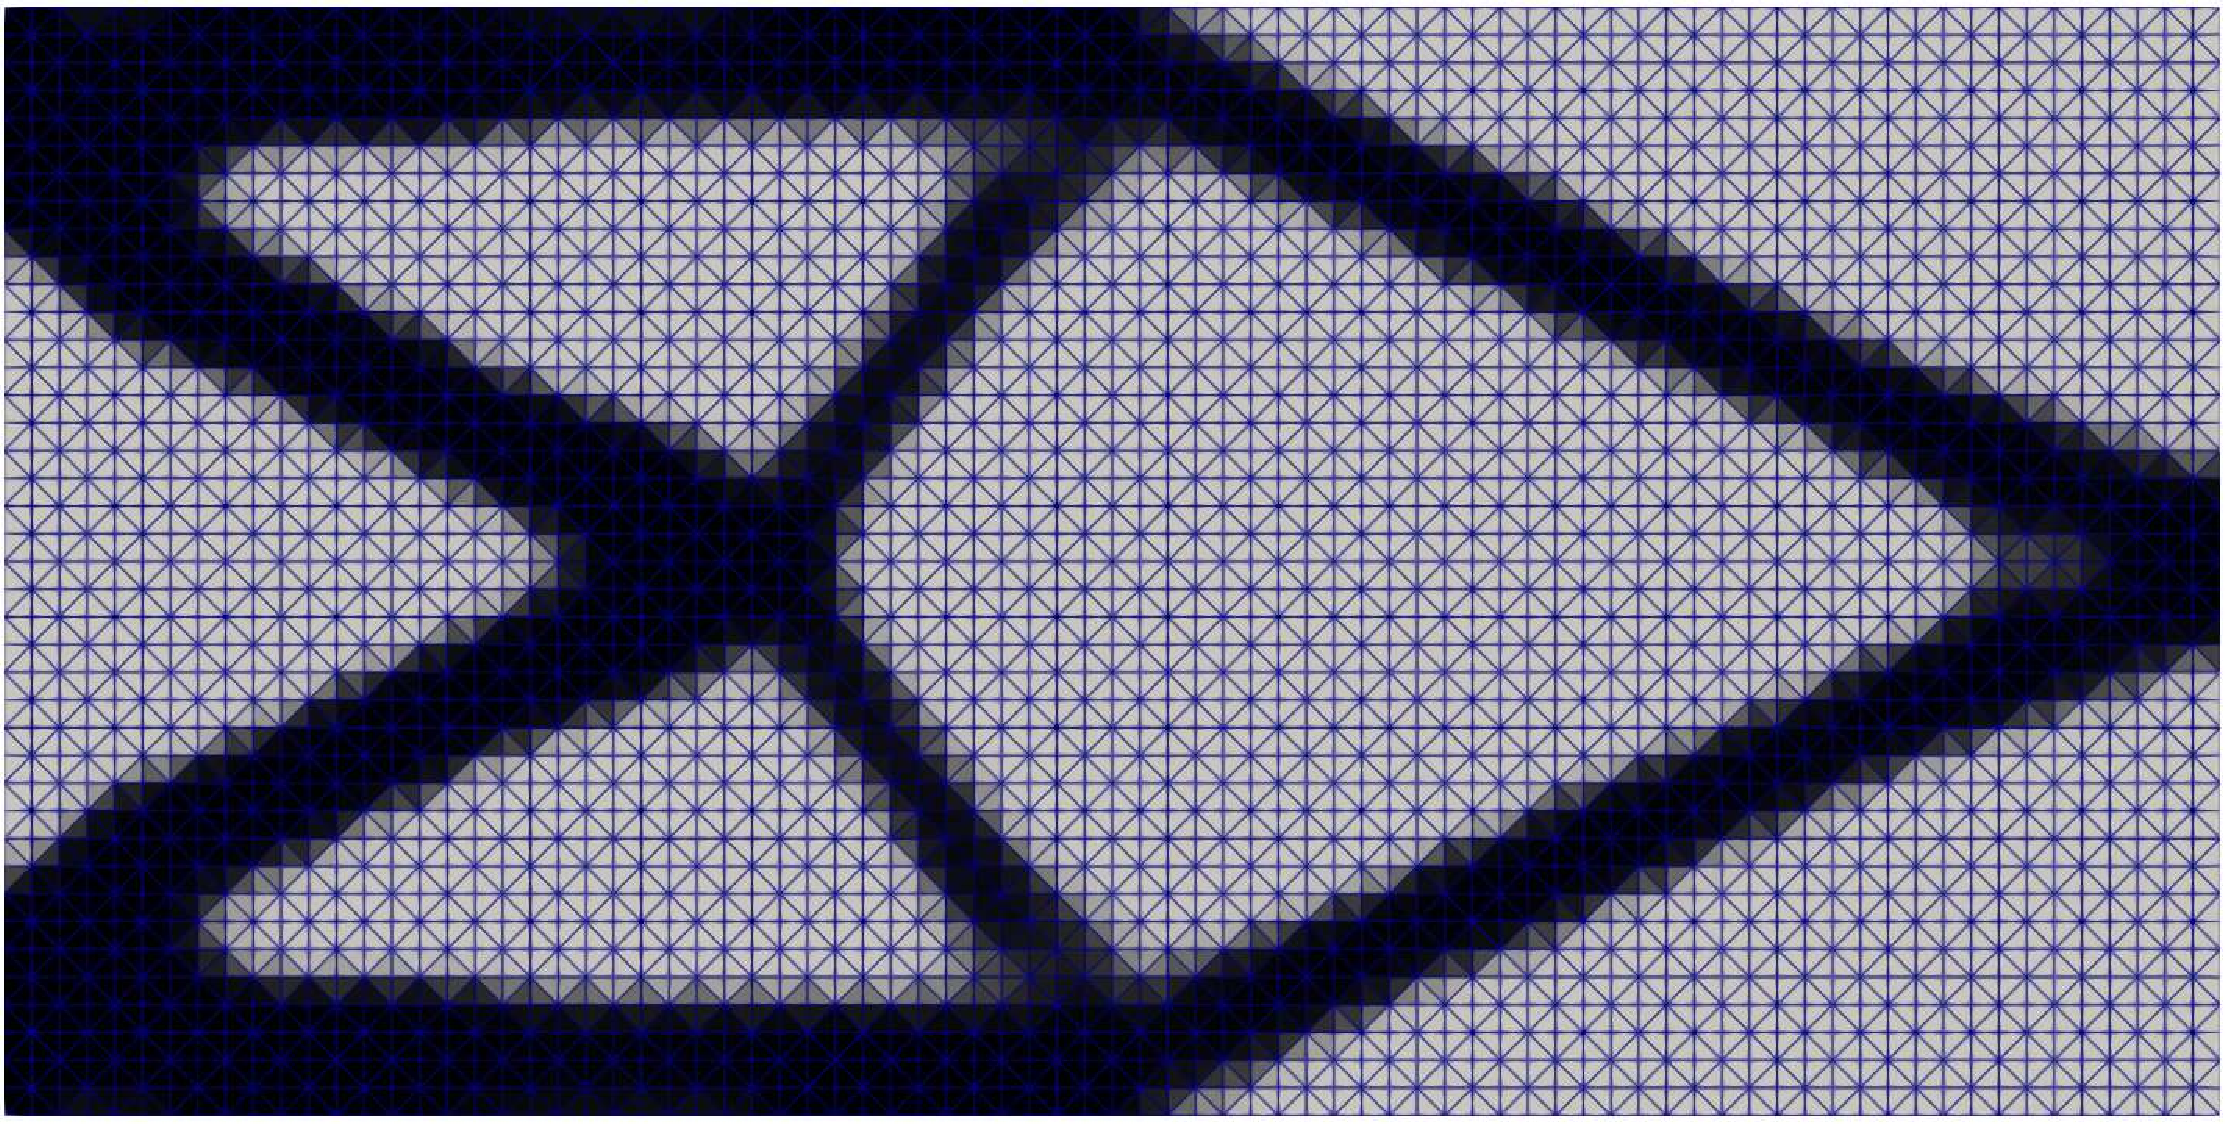
\includegraphics[
					width=0.96\linewidth,
					height=0.205\paperheight,
					keepaspectratio]{stress_topo_disp}
					
					\vspace{0.10em}
					
					{\fontsize{7.0}{8.8}\selectfont\sffamily
						形成清晰 V 型交叉承载构型}
				\end{column}
				
				\begin{column}{0.42\linewidth}\centering
					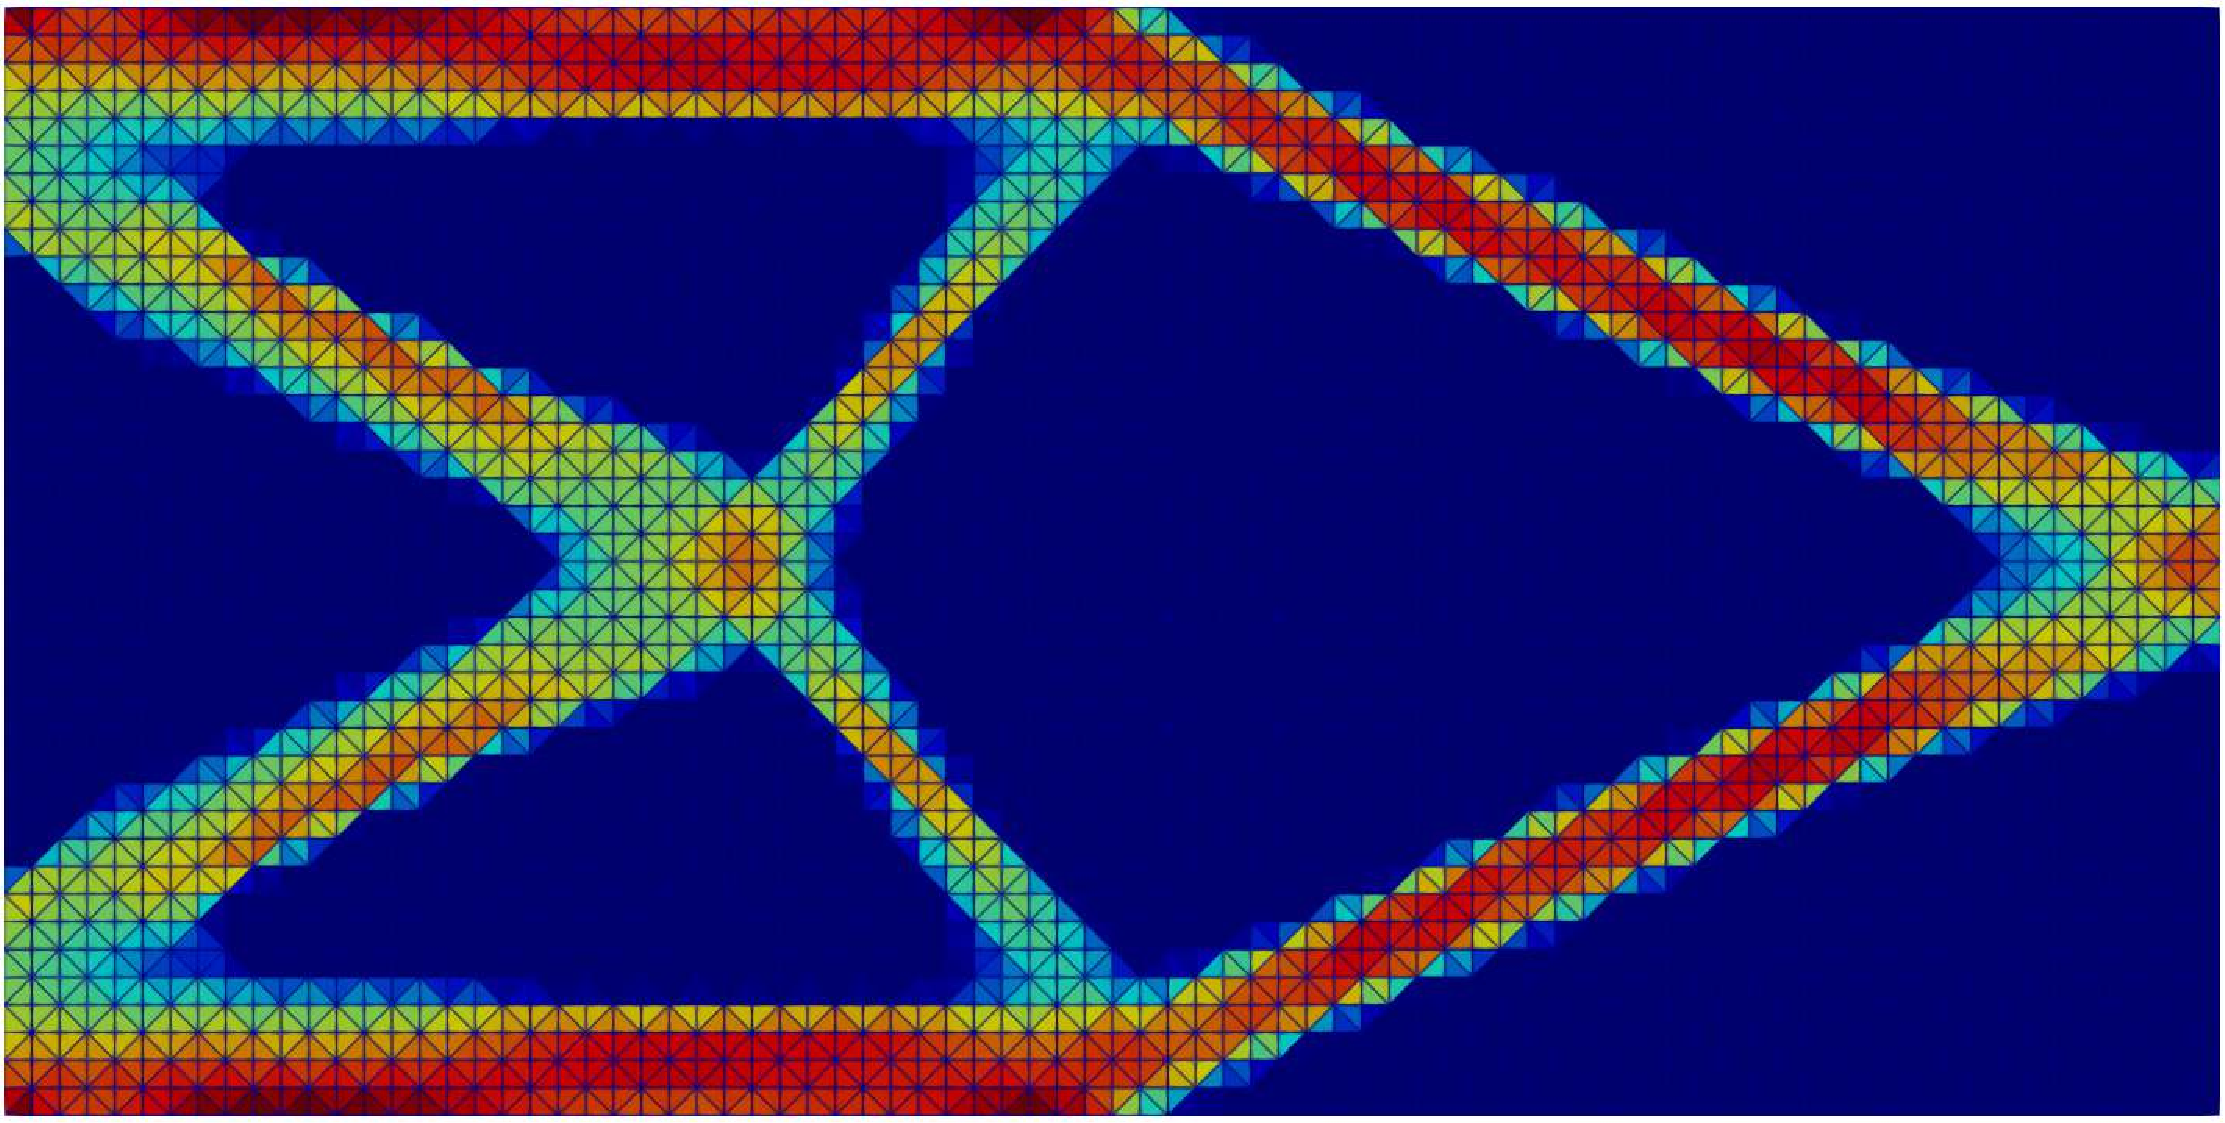
\includegraphics[
					width=0.96\linewidth,
					height=0.205\paperheight,
					keepaspectratio]{stress_vm_disp}
					
					\vspace{0.10em}
					
					{\fontsize{7.0}{8.8}\selectfont\sffamily
						单元间应力跳跃较明显}
				\end{column}
			\end{columns}
			
			\vspace{0.42em}
			
			% ── 第二行：胡张混合法 ────────────────────────────────────
			\begin{columns}[c, totalwidth=\linewidth]
				\begin{column}{0.10\linewidth}\centering
					{\fontsize{8.4}{10}\selectfont\sffamily\bfseries\color{structure.fg}
						胡张\\[2pt]混合法\\[-1pt]
						{\fontsize{6.5}{8}\selectfont \(k=2\)}}
				\end{column}
				
				\begin{column}{0.42\linewidth}\centering
					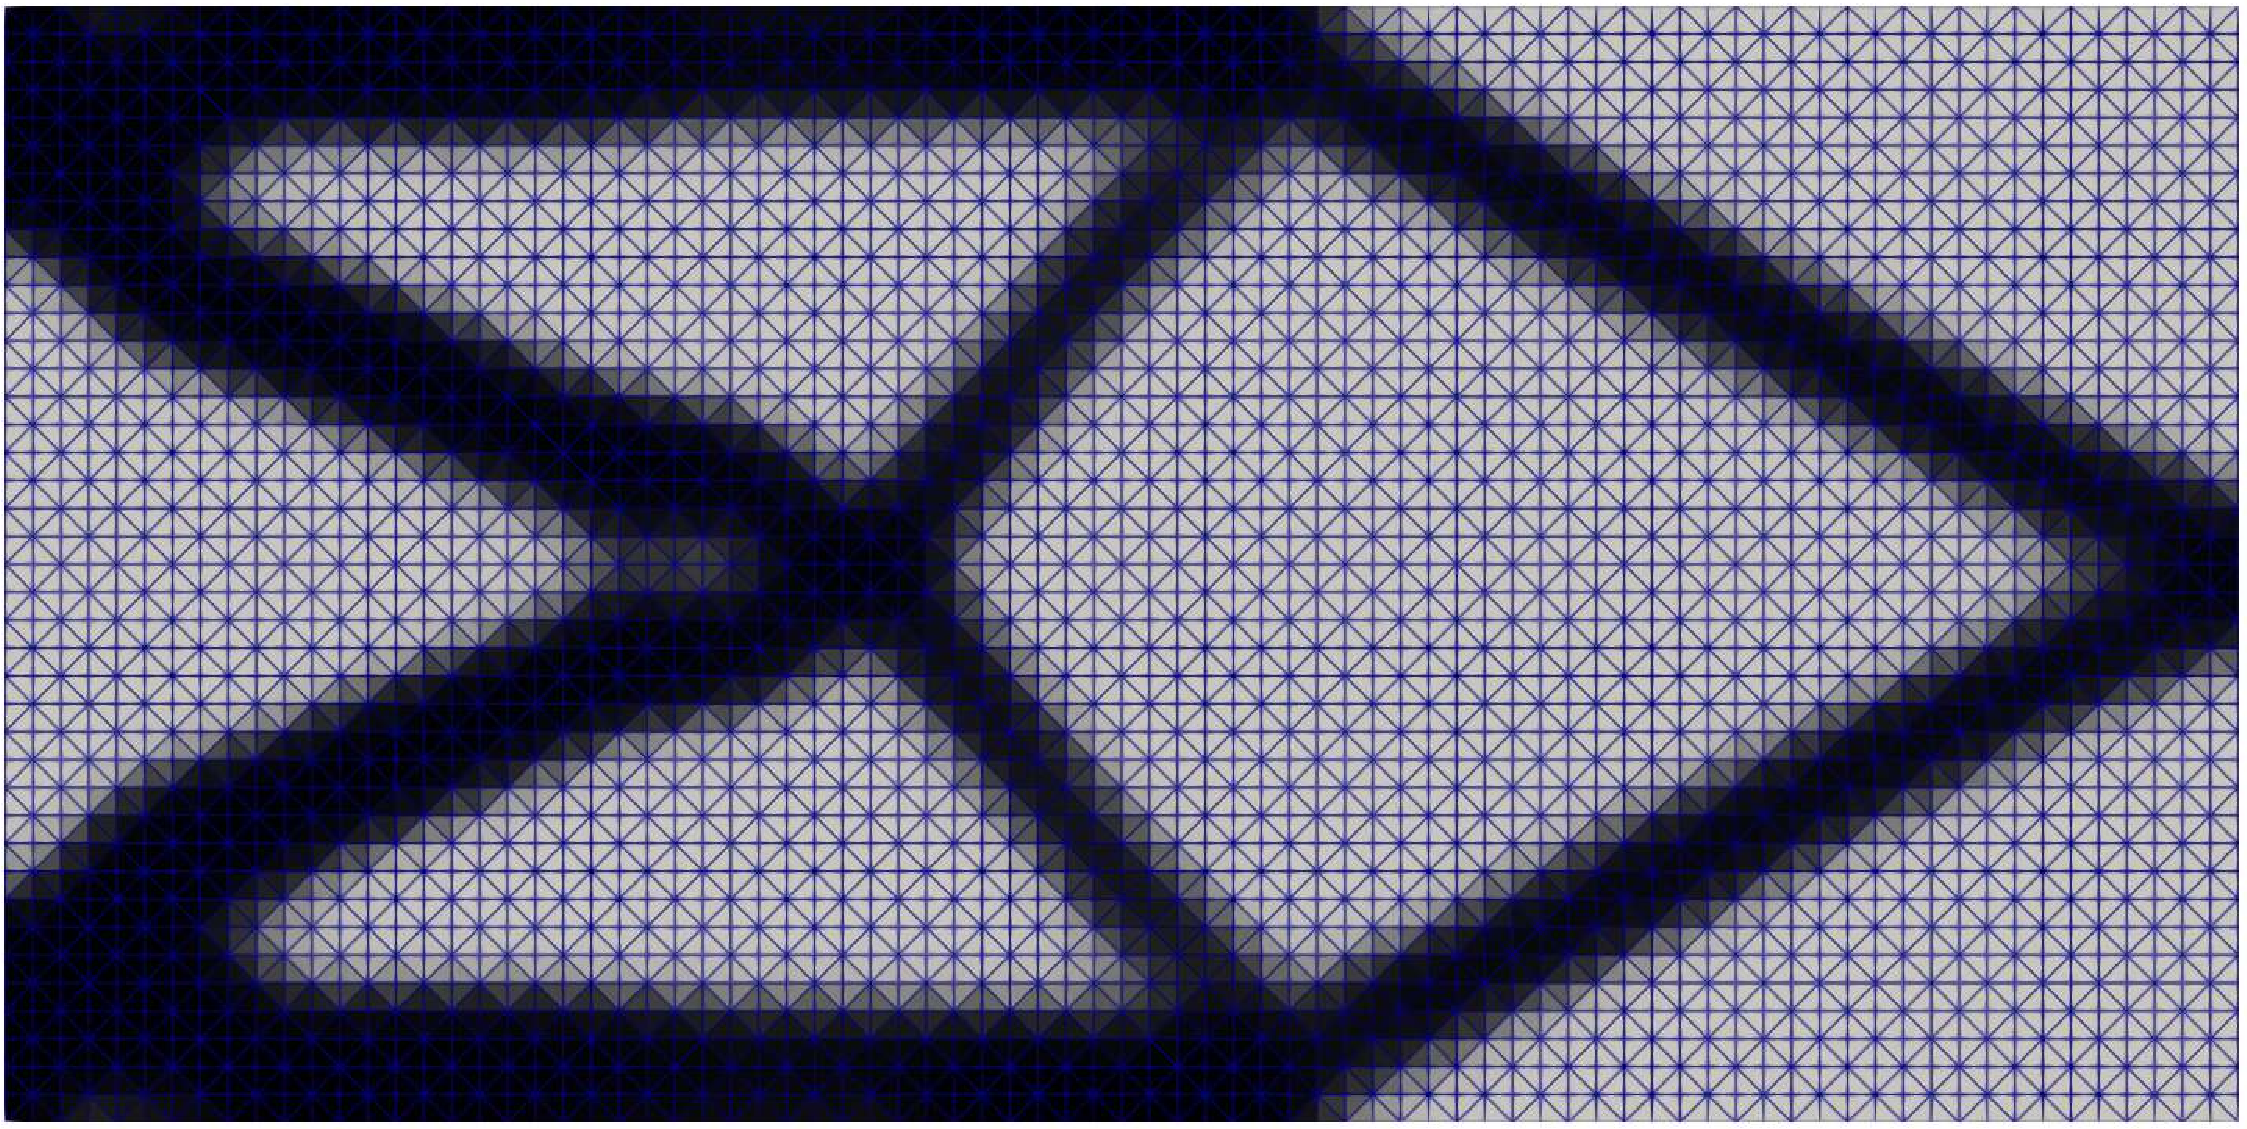
\includegraphics[
					width=0.96\linewidth,
					height=0.205\paperheight,
					keepaspectratio]{stress_topo_mixed}
					
					\vspace{0.10em}
					
					{\fontsize{7.0}{8.8}\selectfont\sffamily
						宏观拓扑构型保持一致}
				\end{column}
				
				\begin{column}{0.42\linewidth}\centering
					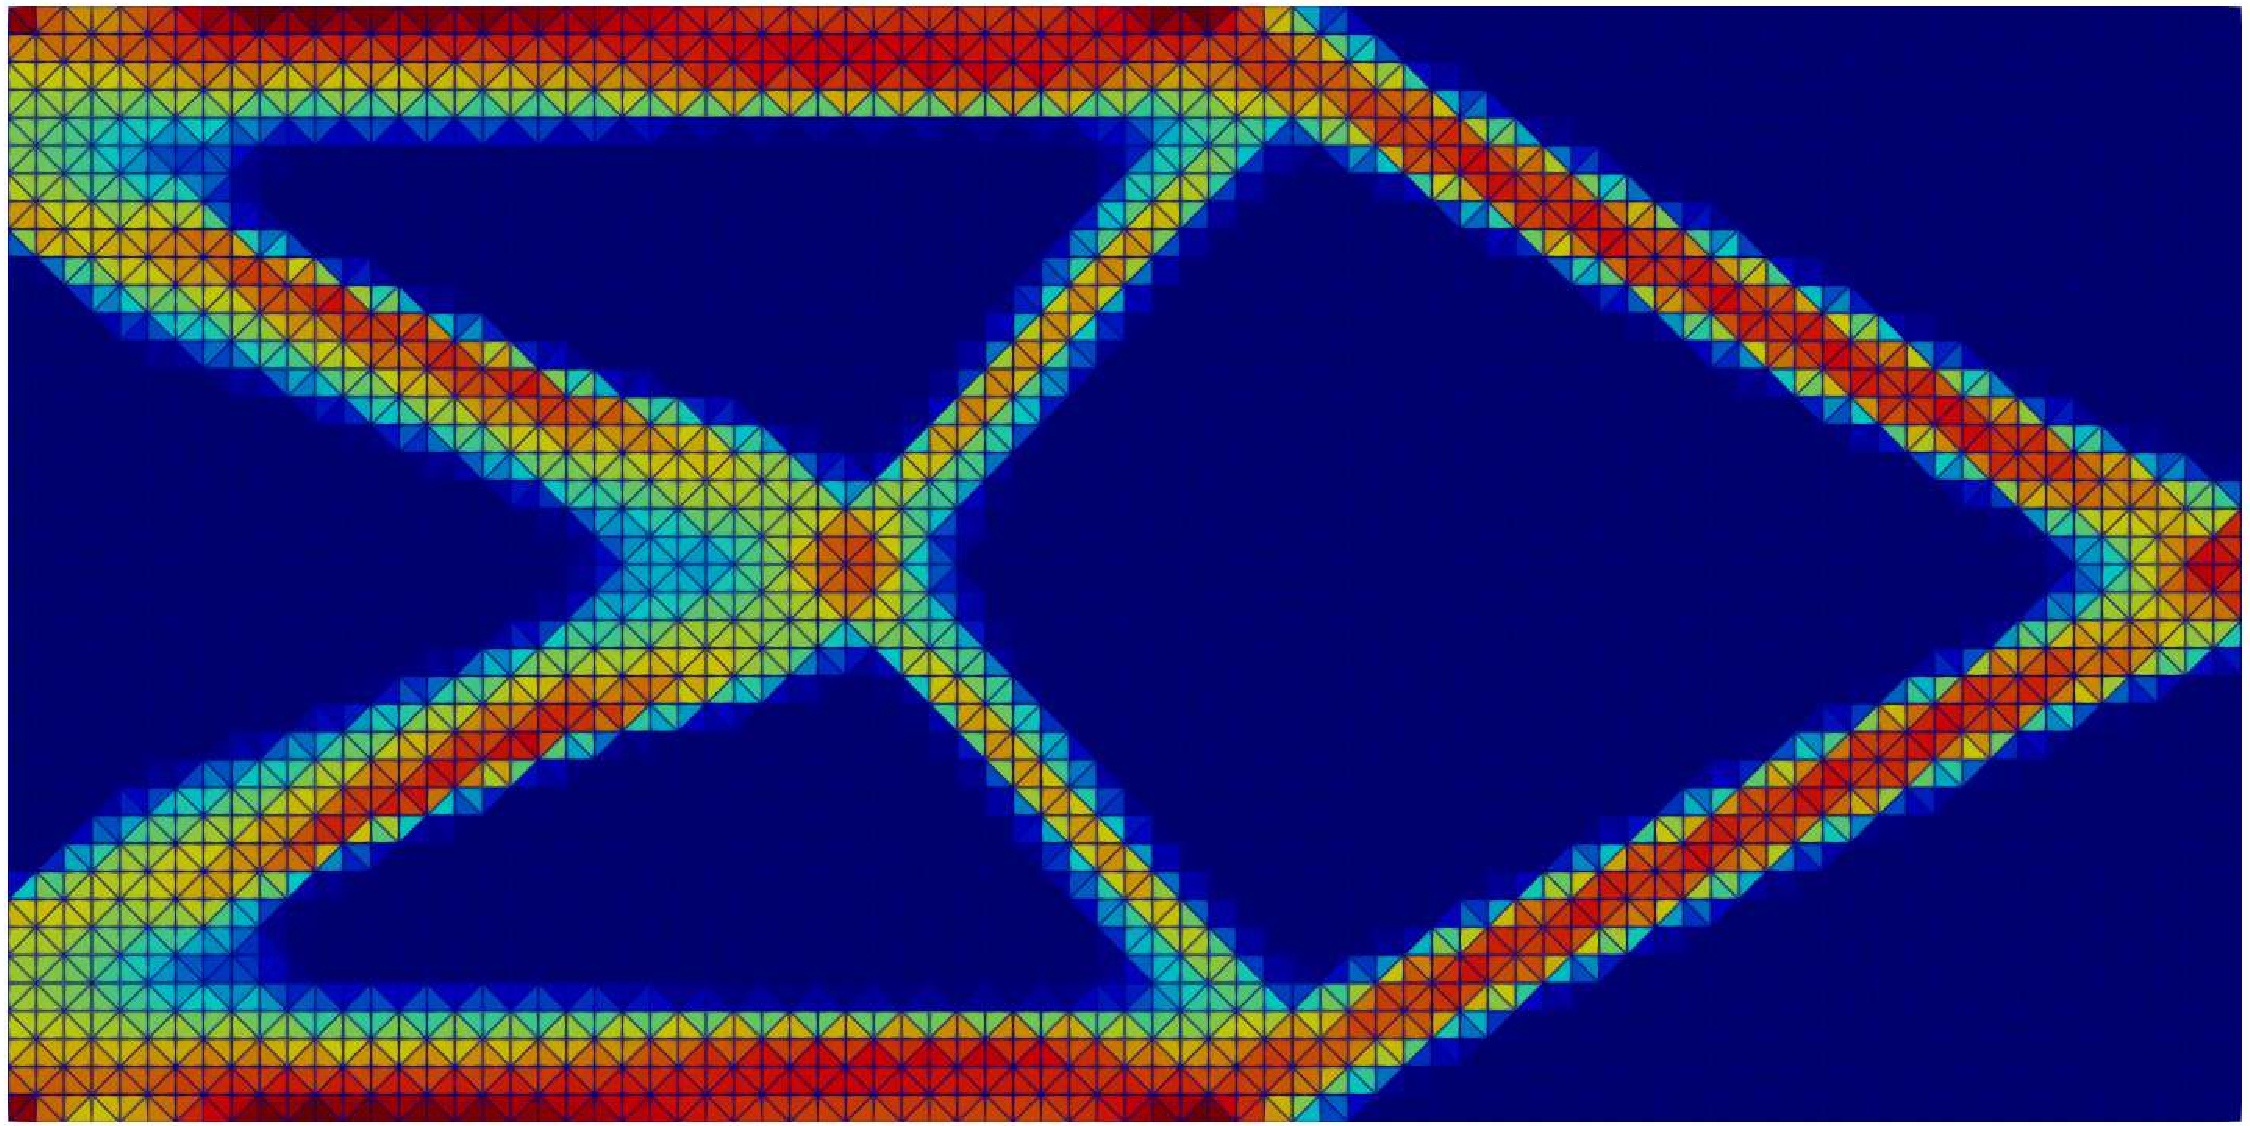
\includegraphics[
					width=0.96\linewidth,
					height=0.205\paperheight,
					keepaspectratio]{stress_vm_mixed}
					
					\vspace{0.10em}
					
					{\fontsize{7.0}{8.8}\selectfont\sffamily
						应力场更平滑，约束评估更可靠}
				\end{column}
			\end{columns}
			
			\vspace{0.35em}
			
			% ── 底部结论条 ───────────────────────────────────────────
			\begin{tcolorbox}[
				colback=structure.fg,
				colframe=structure.fg,
				coltext=white,
				boxrule=0pt,
				arc=3pt,
				top=3pt,
				bottom=3pt,
				left=8pt,
				right=8pt]
				\centering
				{\fontsize{7.35}{9.8}\selectfont\sffamily
					两类方法均得到清晰的 V 型交叉承载构型；但标准位移法应力场易出现单元间非物理跳跃，\\
					胡张混合法基于$H(\text{div})$ 协调应力空间，可获得更平滑连续、约束评估更可靠的局部应力场。}
			\end{tcolorbox}
		}
		
	\end{frame}
	
	
	% ============================================================
	\section{多后端拓扑优化模块化框架 SOPTX}
	% ============================================================
	
	% ============================================================
	%  06-1  研发背景与设计理念
	% ============================================================
	\begin{frame}
		\frametitle{研发背景与设计理念}
		
		\vspace{-2em}
		
		\begin{columns}[t, totalwidth=\linewidth]
			
			% ══════════════════════════════════════════════════════
			%  左列：传统实现瓶颈
			% ══════════════════════════════════════════════════════
			\begin{column}{0.48\linewidth}
				\begin{tcolorbox}[
					title=传统实现瓶颈,
					colback=panelbg, colframe=structure.fg!50,
					colbacktitle=structure.fg, coltitle=white,
					fonttitle=\bfseries, halign title=center,
					boxrule=0.5pt, arc=2pt,
					top=6pt, bottom=6pt, left=6pt, right=6pt,
					toptitle=3pt, bottomtitle=3pt,
					]
					{\fontsize{7.5}{11}\selectfont\sffamily
						\setlength{\parskip}{0pt}
						\textbf{\circnum{1}~架构耦合}\par
						\vspace{2pt}
						物理分析、灵敏度计算与优化更新高度耦合，新模型、新约束与新算法接入成本较高。
						
						\par\vspace{6pt}
						\textbf{\circnum{2}~计算瓶颈}\par
						\vspace{2pt}
						高分辨率与大规模问题中，矩阵组装、方程求解与迭代更新带来显著计算开销。
						
						\par\vspace{6pt}
						\textbf{\circnum{3}~灵敏度实现复杂}\par
						\vspace{2pt}
						局部应力等复杂约束涉及大量梯度计算，手工推导与程序维护成本较高。
					}
				\end{tcolorbox}
			\end{column}
			
			\hfill
			
			% ══════════════════════════════════════════════════════
			%  右列：SOPTX 设计理念
			% ══════════════════════════════════════════════════════
			\begin{column}{0.48\linewidth}
				\begin{tcolorbox}[
					title=SOPTX 设计理念,
					colback=panelbg, colframe=structure.fg!50,
					colbacktitle=structure.fg, coltitle=white,
					fonttitle=\bfseries, halign title=center,
					boxrule=0.5pt, arc=2pt,
					top=6pt, bottom=6pt, left=6pt, right=6pt,
					toptitle=3pt, bottomtitle=3pt,
					]
					{\fontsize{7.5}{11}\selectfont\sffamily
						\setlength{\parskip}{0pt}
						\textbf{\circnum{1}~模块化封装}\par
						\vspace{2pt}
						将材料插值、物理分析、正则化、目标/约束与优化更新封装为独立模块。
						
						\par\vspace{6pt}
						\textbf{\circnum{2}~标准化数据流}\par
						\vspace{2pt}
						设计变量 $\boldsymbol{d}\!\to\!$ 物理密度 $\boldsymbol{\rho}\!\to\!$ 状态变量 $\mathbf{s}\!\to\!$\\ 
						目标/约束 $(J,g)\!\to\!$ 灵敏度 $(\nabla J,\nabla g)$
						
						\par\vspace{6pt}
						\textbf{\circnum{3}~策略可替换}\par
						\vspace{2pt}
						在统一接口下灵活切换有限元离散、过滤策略、灵敏度计算方式与优化算法。
					}
				\end{tcolorbox}
			\end{column}
			
		\end{columns}
		
		\vspace{0.4em}
		
		% ── 底部核心结论强调条 ───────────────────────────────
		\begin{tcolorbox}[
			colback=structure.fg, colframe=structure.fg,
			coltext=white, boxrule=0pt, arc=2pt,
			top=4pt, bottom=4pt, left=8pt, right=8pt,
			]
			\centering\fontsize{8}{11}\selectfont\sffamily\bfseries
			以“分析—优化解耦”为核心，构建面向高阶有限元拓扑优化的模块化软件平台
		\end{tcolorbox}
		
	\end{frame}
	
	% ============================================================
	%  06-2  总体架构与关键技术
	% ============================================================
	\begin{frame}
		\frametitle{总体架构与关键技术}
		
		\vspace{-1.5em}
		
		\begin{columns}[t, totalwidth=\linewidth]
			
			% ══════════════════════════════════════════════════════
			%  左列：总体架构（三层）
			% ══════════════════════════════════════════════════════
			\begin{column}{0.48\linewidth}
				\begin{tcolorbox}[
					title=总体架构,
					equal height group=row032,       
					colback=panelbg, colframe=structure.fg!50,
					colbacktitle=structure.fg, coltitle=white,
					fonttitle=\bfseries, halign title=center,
					boxrule=0.5pt, arc=2pt,
					top=6pt, bottom=6pt, left=6pt, right=6pt,
					toptitle=3pt, bottomtitle=3pt,
					]
					{\fontsize{7.5}{11}\selectfont\sffamily
						\setlength{\parskip}{0pt}
						\textbf{\circnum{1}~用户交互层}\par
						\vspace{2pt}
						Python API / 脚本入口；算例模型与参数配置；结果后处理、可视化与导出。
						
						\par\vspace{4pt}
						\textbf{\circnum{2}~核心算法层}\par
						\vspace{2pt}
						围绕拓扑优化闭环组织插值、分析、正则化与优化模块，实现平台主流程编排。
						
						\par\vspace{4pt}
						\textbf{\circnum{3}~基础后端层}\par
						\vspace{2pt}
						依托 FEALPy 的网格、函数空间、数值积分、矩阵组装、求解器与多后端张量计算能力。
					}
				\end{tcolorbox}
			\end{column}
			
			\hfill
			
			% ══════════════════════════════════════════════════════
			%  右列：关键技术
			% ══════════════════════════════════════════════════════
			\begin{column}{0.48\linewidth}
				\begin{tcolorbox}[
					title=关键技术,
					equal height group=row032,  
					colback=panelbg, colframe=structure.fg!50,
					colbacktitle=structure.fg, coltitle=white,
					fonttitle=\bfseries, halign title=center,
					boxrule=0.5pt, arc=2pt,
					top=6pt, bottom=6pt, left=6pt, right=6pt,
					toptitle=3pt, bottomtitle=3pt,
					]
					{\fontsize{7.5}{11}\selectfont\sffamily
						\setlength{\parskip}{0pt}
						\textbf{\circnum{1}~高效矩阵组装}\par
						\vspace{2pt}
						通过解析预计算、张量收缩与算子缓存，降低拓扑优化迭代中的重复装配开销。
						
						\par\vspace{4pt}
						\textbf{\circnum{2}~自动微分灵敏度}\par
						\vspace{2pt}
						依托 PyTorch / JAX 后端，实现复杂目标与约束的梯度自动计算。
						
						\par\vspace{4pt}
						\textbf{\circnum{3}~多后端与异构执行}\par
						\vspace{2pt}
						支持 NumPy / PyTorch / JAX 后端切换，支撑 CPU / GPU 可移植计算。
					}
				\end{tcolorbox}
			\end{column}
			
		\end{columns}
		
		\vspace{0.4em}
		
		% ── 底部核心结论强调条 ───────────────────────────────
		\begin{tcolorbox}[
			colback=structure.fg, colframe=structure.fg,
			coltext=white, boxrule=0pt, arc=2pt,
			top=4pt, bottom=4pt, left=8pt, right=8pt,
			]
			\centering\fontsize{8}{11}\selectfont\sffamily\bfseries
			通过分层架构与关键技术集成，为高阶有限元拓扑优化提供高效、可扩展的软件支撑。
		\end{tcolorbox}
		
	\end{frame}
	
	% ============================================================
	%  06-3  核心模块与计算闭环
	% ============================================================
	\begin{frame}
		\frametitle{核心模块与计算闭环}
		
		\vspace{-0.5em}
		
		% ── 主体内容：2x2 模块卡片排版 ──────────────────────────────────
		\begin{columns}[T, totalwidth=\linewidth]
			
			% ─── 左列：模块 01 与 03 ──────────────────────────────
			\begin{column}{0.485\linewidth}
				
				% 模块 01
				\begin{tcolorbox}[
					colback=white, colframe=structure.fg!50,
					colbacktitle=structure.fg, coltitle=white,
					fonttitle=\fontsize{8}{10}\selectfont\bfseries\sffamily,
					title={\circnum{01}\enspace 插值模块},
					arc=3pt, boxrule=0.5pt,
					toptitle=1pt, bottomtitle=1pt,
					top=6pt, bottom=6pt, left=8pt, right=8pt,
					height=0.28\paperheight, valign=center]
					{\fontsize{7.5}{11}\selectfont\sffamily
						建立设计变量到材料属性的映射，\par
						\vspace{3pt}
						为有限元分析提供物理密度与材料刚度。}
				\end{tcolorbox}
				
				% 模块 03
				\begin{tcolorbox}[
					colback=white, colframe=structure.fg!50,
					colbacktitle=structure.fg, coltitle=white,
					fonttitle=\fontsize{8}{10}\selectfont\bfseries\sffamily,
					title={\circnum{03}\enspace 正则化模块},
					arc=3pt, boxrule=0.5pt,
					toptitle=1pt, bottomtitle=1pt,
					top=6pt, bottom=6pt, left=8pt, right=8pt,
					height=0.28\paperheight, valign=center]
					{\fontsize{7.5}{11}\selectfont\sffamily
						通过过滤与投影控制最小特征尺度，\par
						\vspace{3pt}
						改善拓扑稳定性与边界清晰度。}
				\end{tcolorbox}
				
			\end{column}
			
			% ─── 右列：模块 02 与 04 ──────────────────────────────
			\begin{column}{0.485\linewidth}
				
				% 模块 02
				\begin{tcolorbox}[
					colback=white, colframe=structure.fg!50,
					colbacktitle=structure.fg, coltitle=white,
					fonttitle=\fontsize{8}{10}\selectfont\bfseries\sffamily,
					title={\circnum{02}\enspace 分析模块},
					arc=3pt, boxrule=0.5pt,
					toptitle=1pt, bottomtitle=1pt,
					top=6pt, bottom=6pt, left=8pt, right=8pt,
					height=0.28\paperheight, valign=center]
					{\fontsize{7.5}{11}\selectfont\sffamily
						封装有限元离散、矩阵组装与状态求解，\par
						\vspace{3pt}
						获得位移、应力等状态场量。}
				\end{tcolorbox}
				
				% 模块 04
				\begin{tcolorbox}[
					colback=white, colframe=structure.fg!50,
					colbacktitle=structure.fg, coltitle=white,
					fonttitle=\fontsize{8}{10}\selectfont\bfseries\sffamily,
					title={\circnum{04}\enspace 优化模块},
					arc=3pt, boxrule=0.5pt,
					toptitle=1pt, bottomtitle=1pt,
					top=6pt, bottom=6pt, left=8pt, right=8pt,
					height=0.28\paperheight, valign=center]
					{\fontsize{7.5}{11}\selectfont\sffamily
						统一管理目标、约束、灵敏度与设计更新，\par
						\vspace{3pt}
						驱动拓扑构型迭代演化。}
				\end{tcolorbox}
				
			\end{column}
			
		\end{columns}
		
		% ── 底部核心结论强调条 ───────────────────────────────
		\begin{tcolorbox}[
			colback=structure.fg, colframe=structure.fg,
			coltext=white, boxrule=0pt, arc=3pt,
			top=4pt, bottom=4pt, left=8pt, right=8pt,
			]
			\centering\fontsize{8}{10}\selectfont\sffamily
			四大模块共同支撑“正则化映射—材料插值—状态分析—灵敏度反馈—优化更新”
			的拓扑优化计算闭环。
		\end{tcolorbox}
		
	\end{frame}
	
	% ============================================================
	%  06-4  高效矩阵组装与性能提升
	% ============================================================
	
	\begin{frame}
		\frametitle{高效矩阵组装与算子缓存机制}
		
		% ── 顶部总述条 ──────────────────────────────────────
		\begin{tcolorbox}[
			colback=panelbg, colframe=structure.fg!40,
			arc=3pt, boxrule=0.5pt,
			top=3pt, bottom=3pt, left=8pt, right=8pt]
			{\fontsize{8}{12}\selectfont\sffamily
				针对拓扑优化迭代中的重复矩阵装配，SOPTX 通过快速组装与算子缓存机制，
				将局部刚度计算转化为可复用的张量化过程。}
		\end{tcolorbox}
		
		% ══════════════════════════════════════════════════════════
		%  中部：表 6.1（裸表）
		% ══════════════════════════════════════════════════════════
		\begin{center}
			{\fontsize{8.5}{11}\selectfont\sffamily\bfseries
				三维悬臂梁算例中不同矩阵组装策略的性能对比（单位：s）}
			
			\vspace{6pt}
			
			{\fontsize{8.5}{12}\selectfont\sffamily
				\renewcommand{\arraystretch}{1.30}
				\begin{tabular}{@{}l@{\hspace{2.8em}}c@{\hspace{2.8em}}c@{\hspace{2.8em}}c@{}}
					\toprule
					\textbf{矩阵组装方式} & \textbf{首次组装} & \textbf{后续平均组装} & \textbf{总耗时} \\
					\midrule
					标准组装（基线）       & 1.053 & 0.787          & 92.109          \\
					数值求积快速组装       & 0.281 & 0.182          & \textbf{57.538} \\
					解析预计算快速组装     & 28.909 & \textbf{0.177} & 113.720          \\
					\bottomrule
			\end{tabular}}
		\end{center}
		
		% ══════════════════════════════════════════════════════════
		%  底部：关键结论（一栏三点）
		% ══════════════════════════════════════════════════════════
		\begin{tcolorbox}[
			colback=structure.fg, colframe=structure.fg,
			coltext=white, boxrule=0pt, arc=3pt,
			top=4pt, bottom=4pt, left=8pt, right=8pt]
			{\fontsize{7.5}{11}\selectfont\sffamily
				\setlength{\parskip}{0pt}
				\textbf{\circnum{1} 总耗时最优：}数值求积快速组装总耗时由 \textbf{92.109\,s} 降至 \textbf{57.538\,s}，整体加速约 \textbf{1.6 倍}。
				
				\textbf{\circnum{2} 后续装配加速：}数值求积组装平均耗时降至 \textbf{0.182\,s}，较标准组装的 \textbf{0.787\,s} 提升约 \textbf{4.3 倍}。
				
				\textbf{\circnum{3} 缓存复用优势：}解析预计算后续组装最低，为 \textbf{0.177\,s}，提升约 \textbf{4.4 倍}；但首次开销为 \textbf{28.909\,s}。
			}
		\end{tcolorbox}
		
	\end{frame}
	
	% ============================================================
	%  06-5  自动微分灵敏度分析
	% ============================================================
	
	\begin{frame}
		\frametitle{自动微分灵敏度分析}
		
		% ── 顶部总述条 ──────────────────────────────────────
		\begin{tcolorbox}[
			colback=panelbg, colframe=structure.fg!40,
			arc=3pt, boxrule=0.5pt,
			top=3pt, bottom=3pt, left=8pt, right=8pt]
			{\fontsize{8}{12}\selectfont\sffamily
				SOPTX 提供手动解析与自动微分两类灵敏度路径，
				并从拓扑结果与计算开销两方面验证自动微分机制的可用性。}
		\end{tcolorbox}
		
		% ============================================================
		% Overlay 1：拓扑构型一致性
		% ============================================================
		\only<1>{
			
			\begin{center}
				{\fontsize{8.5}{11}\selectfont\sffamily\bfseries
					不同灵敏度计算路径下三维悬臂梁最终拓扑构型}
			\end{center}
			
			\begin{columns}[T, totalwidth=\linewidth]
				
				\begin{column}{0.48\linewidth}
					\centering
					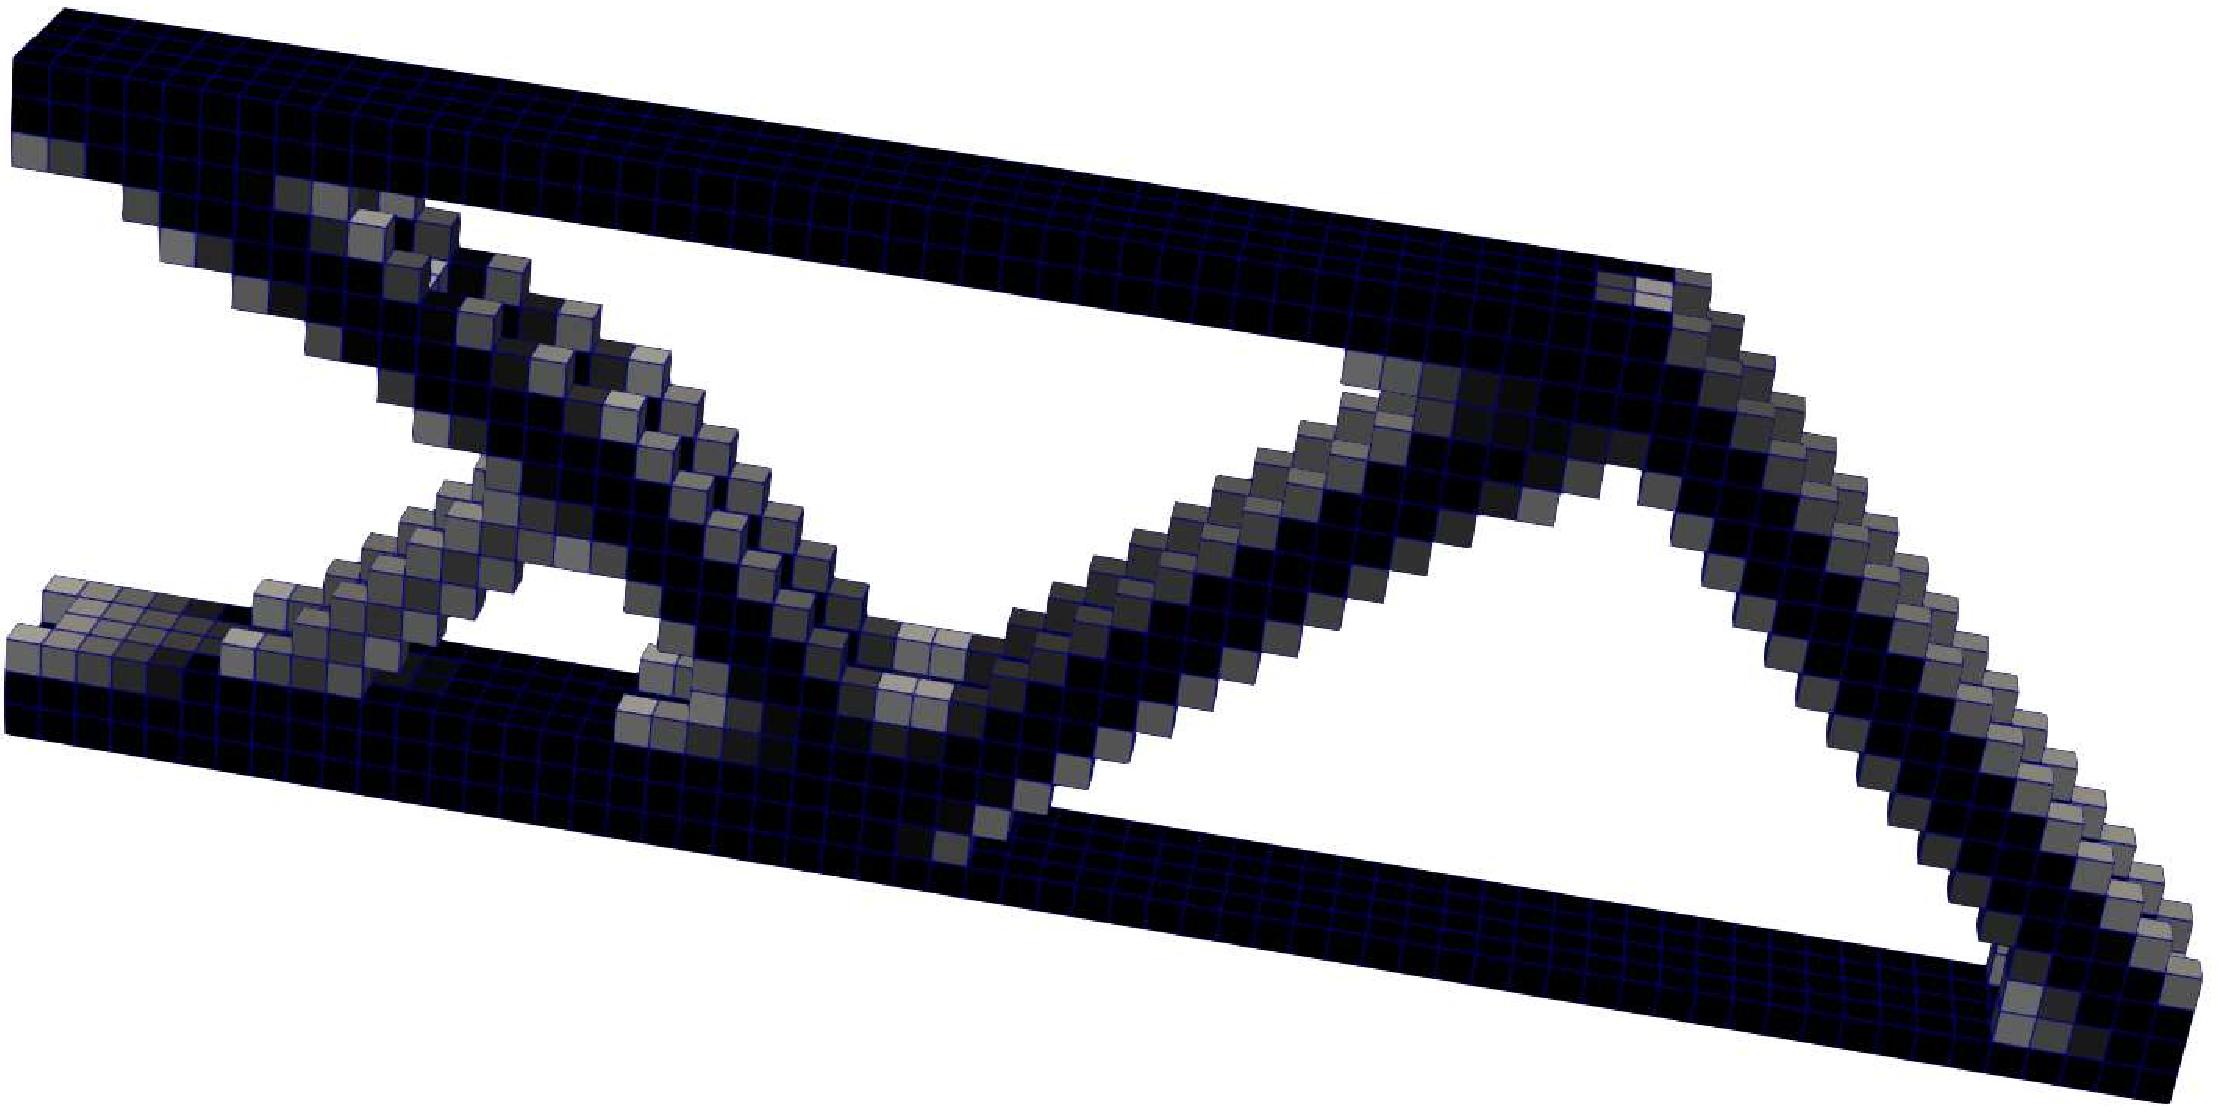
\includegraphics[width=0.75\linewidth,
					height=0.32\paperheight, keepaspectratio]{topo_sens_manual}
					
					{\fontsize{8}{11}\selectfont\sffamily (a)\enspace 手动解析}
				\end{column}
				
				\begin{column}{0.48\linewidth}
					\centering
					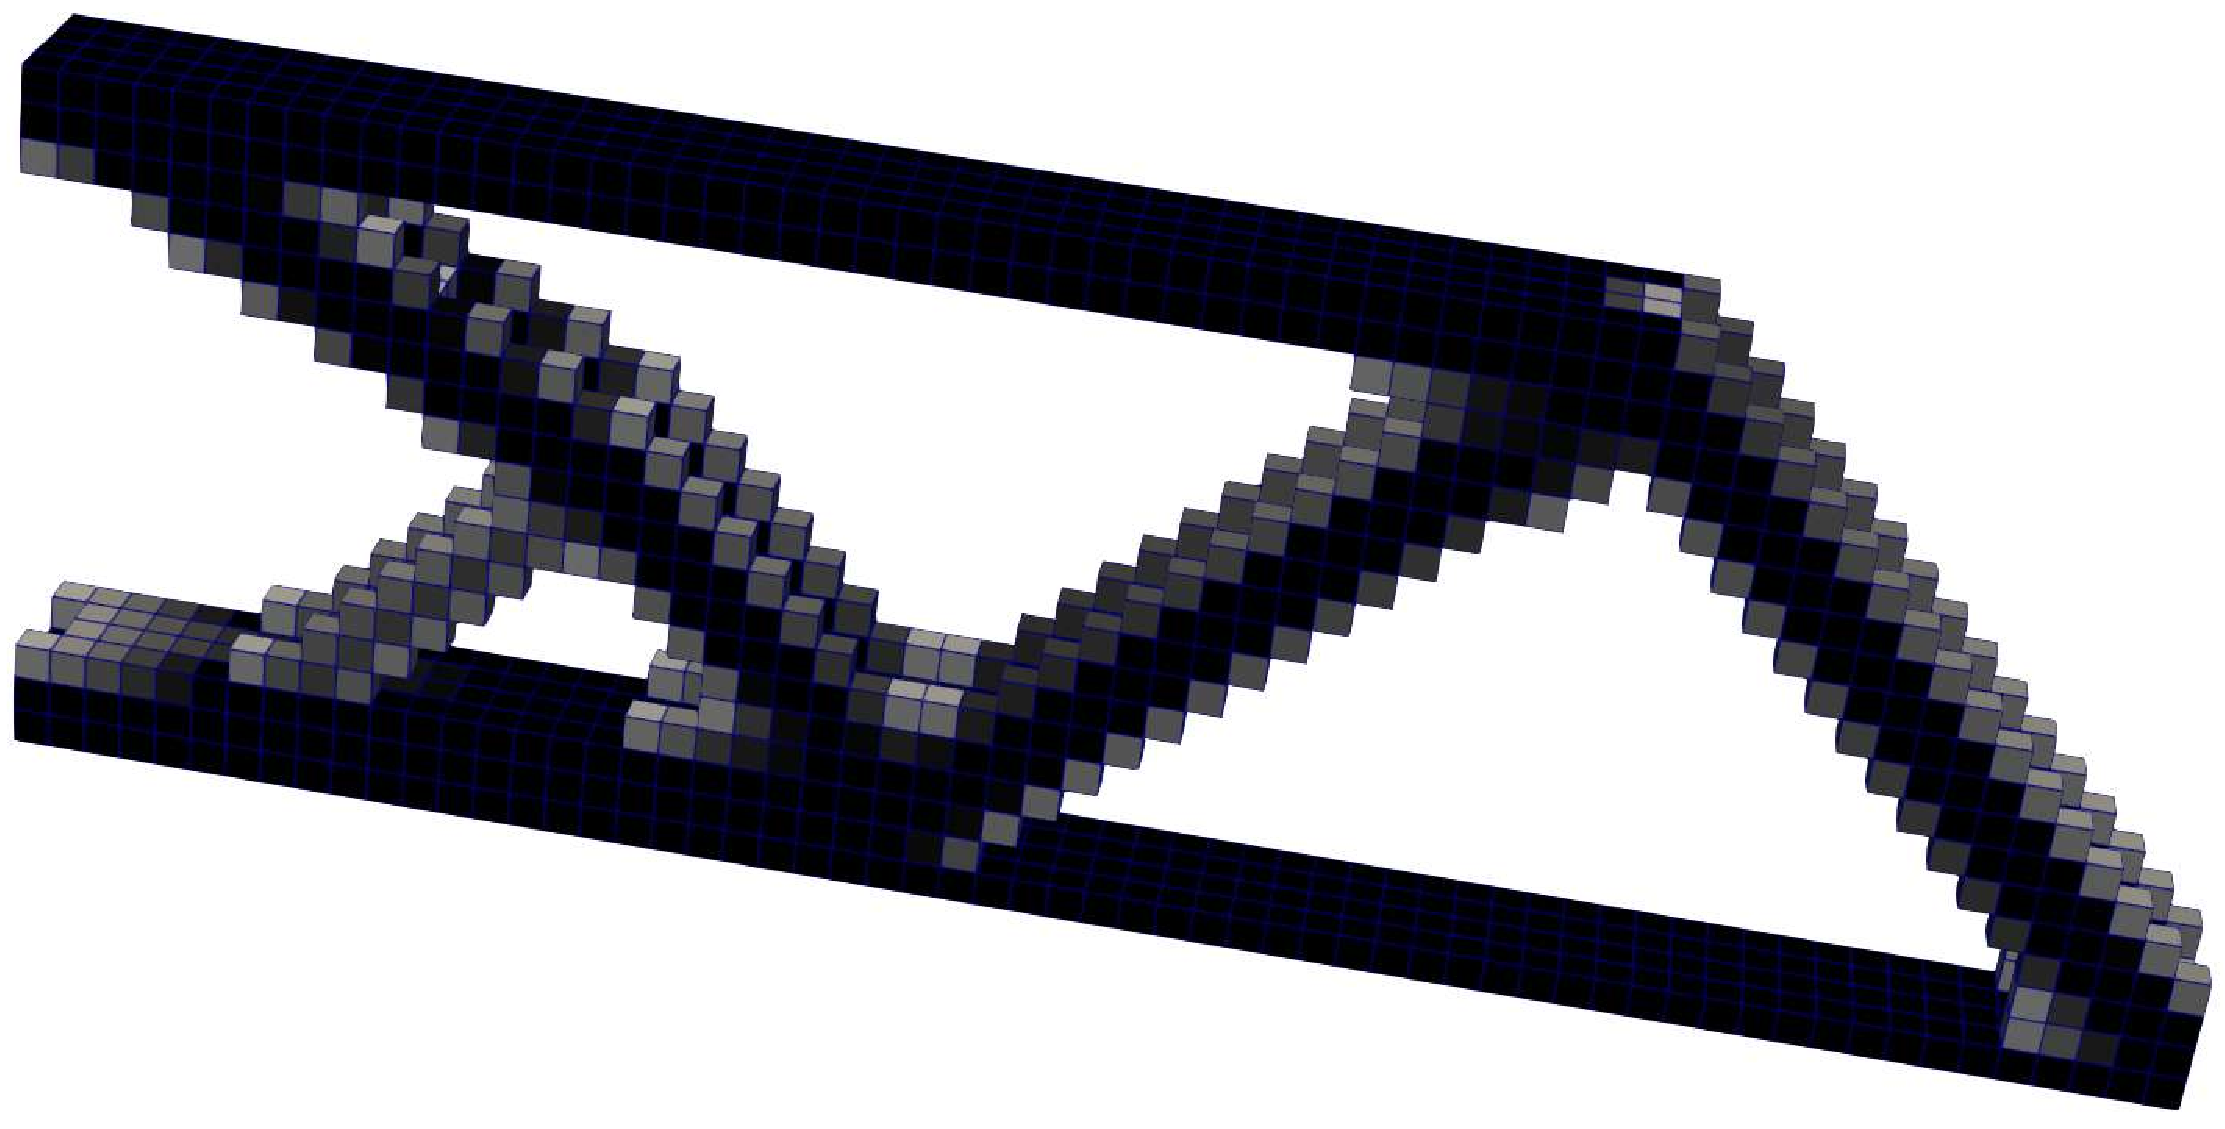
\includegraphics[width=0.75\linewidth,
					height=0.32\paperheight, keepaspectratio]{topo_sens_auto}
					
					{\fontsize{8}{11}\selectfont\sffamily (b)\enspace 自动微分}
				\end{column}
				
			\end{columns}
			
			\begin{tcolorbox}[
				colback=structure.fg, colframe=structure.fg,
				coltext=white, boxrule=0pt, arc=3pt,
				top=4pt, bottom=4pt, left=8pt, right=8pt]
				{\fontsize{7.5}{11}\selectfont\sffamily
					\setlength{\parskip}{0pt}
					\textbf{\circnum{1} 构型一致：}手动解析与自动微分得到主承载路径高度一致的三维拓扑构型。
					
					\textbf{\circnum{2} 扩展便捷：}自动微分降低复杂目标与约束泛函的梯度推导、编码与维护成本。
				}
				
			\end{tcolorbox}
		}
		
		% ============================================================
		% Overlay 2：计算耗时一致性
		% ============================================================
		\only<2>{
			
			\begin{center}
				{\fontsize{8.5}{12}\selectfont\sffamily\bfseries
					不同灵敏度计算路径下三维悬臂梁优化问题耗时对比（单位：s）}
			\end{center}
				
				\centering
				{\fontsize{8.5}{12}\selectfont\sffamily
					\begin{tabular}{lcccc}
						\toprule
						\textbf{灵敏度路径}
						& \textbf{迭代次数}
						& \textbf{总耗时}
						& \textbf{首次迭代耗时}
						& \textbf{后续平均耗时} \\
						\midrule
						手动解析
						& 54
						& 36.627
						& 1.264
						& 0.667 \\
						自动微分
						& 54
						& 36.873
						& 1.460
						& 0.668 \\
						\bottomrule
					\end{tabular}
				}
			
			\begin{tcolorbox}[
				colback=structure.fg, colframe=structure.fg,
				coltext=white, boxrule=0pt, arc=3pt,
				top=4pt, bottom=4pt, left=8pt, right=8pt]
				{\fontsize{7.5}{11}\selectfont\sffamily
					\setlength{\parskip}{0pt}
					\textbf{\circnum{1} 总耗时接近：}自动微分总耗时仅由 \textbf{36.627\,s} 增至 \textbf{36.873\,s}，额外开销约 \textbf{0.246\,s}，约 \textbf{0.67\%}。
					
					\textbf{\circnum{2} 稳态开销一致：}后续平均迭代耗时分别为 \textbf{0.667\,s} 与 \textbf{0.668\,s}，差异约 \textbf{0.15\%}。
				}
				
			\end{tcolorbox}
		}
		
	\end{frame}
	
	% ============================================================
	%  06-6  多后端拓扑结果一致性
	% ============================================================
	
	\begin{frame}
		\frametitle{多后端拓扑结果一致性}
		
		% ── 顶部总述条 ──────────────────────────────────────
		\begin{tcolorbox}[
			colback=panelbg, colframe=structure.fg!40,
			arc=3pt, boxrule=0.5pt,
			top=3pt, bottom=3pt, left=8pt, right=8pt]
			{\fontsize{8}{12}\selectfont\sffamily
				SOPTX 依托统一张量抽象接口，实现 NumPy、PyTorch 与 JAX 后端切换，
				并从最终构型与收敛历程两方面验证跨后端结果一致性。}
		\end{tcolorbox}
		
		% ============================================================
		% Overlay 1：最终拓扑构型一致性
		% ============================================================
		\only<1>{
			
			\begin{center}
				{\fontsize{8.5}{11}\selectfont\sffamily\bfseries
					不同张量后端下三维悬臂梁最终拓扑构型}
			\end{center}
			
			\vspace{-0.2em}
			
			\begin{columns}[T, totalwidth=\linewidth]
				
				\begin{column}{0.32\linewidth}
					\centering
					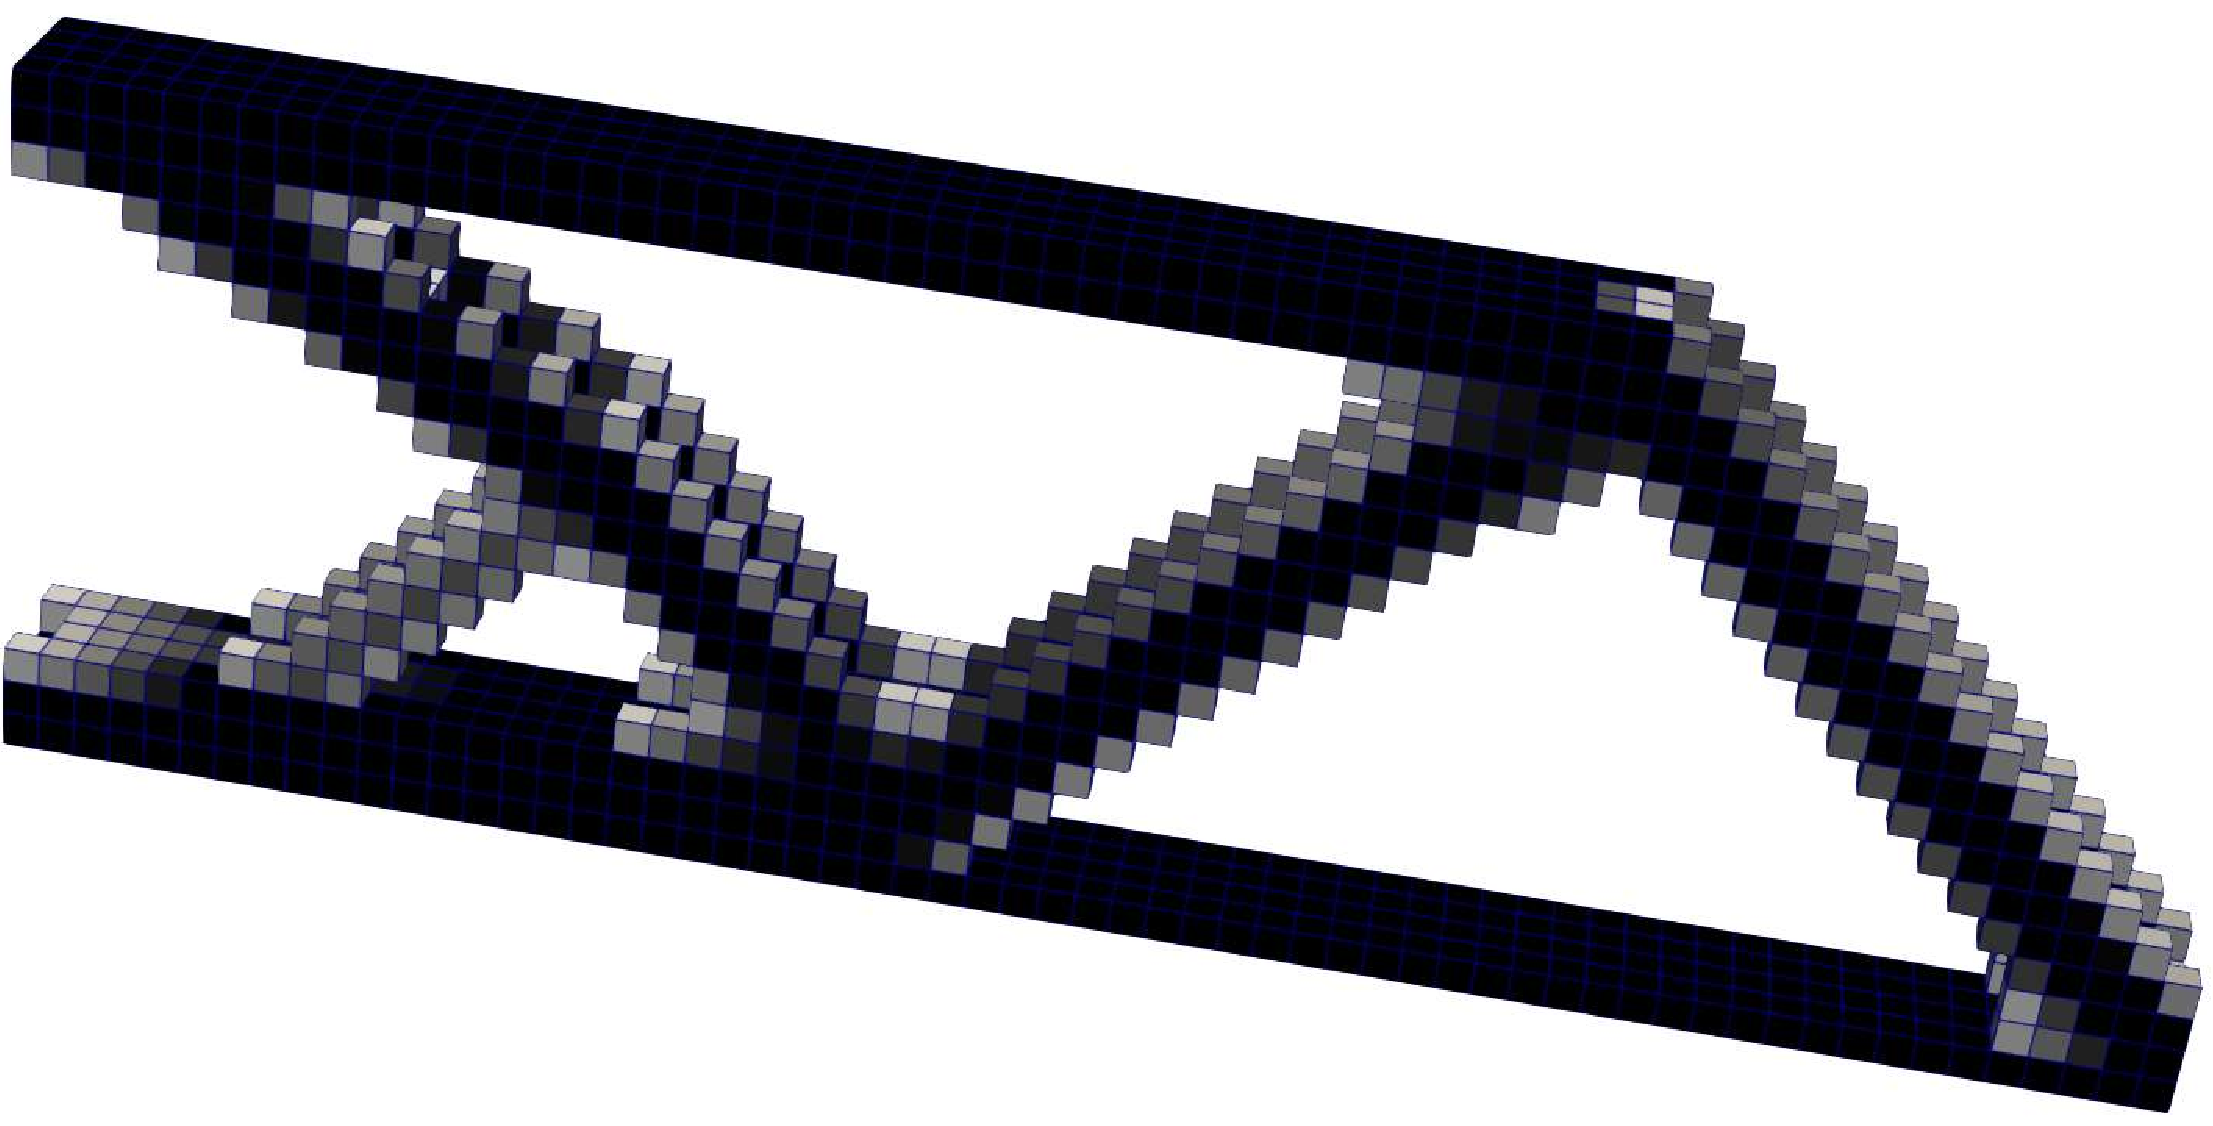
\includegraphics[width=0.95\linewidth,
					height=0.30\paperheight, keepaspectratio]{topo_backend_numpy}
					
					{\fontsize{8}{11}\selectfont\sffamily (a)\enspace NumPy}
				\end{column}
				
				\begin{column}{0.32\linewidth}
					\centering
					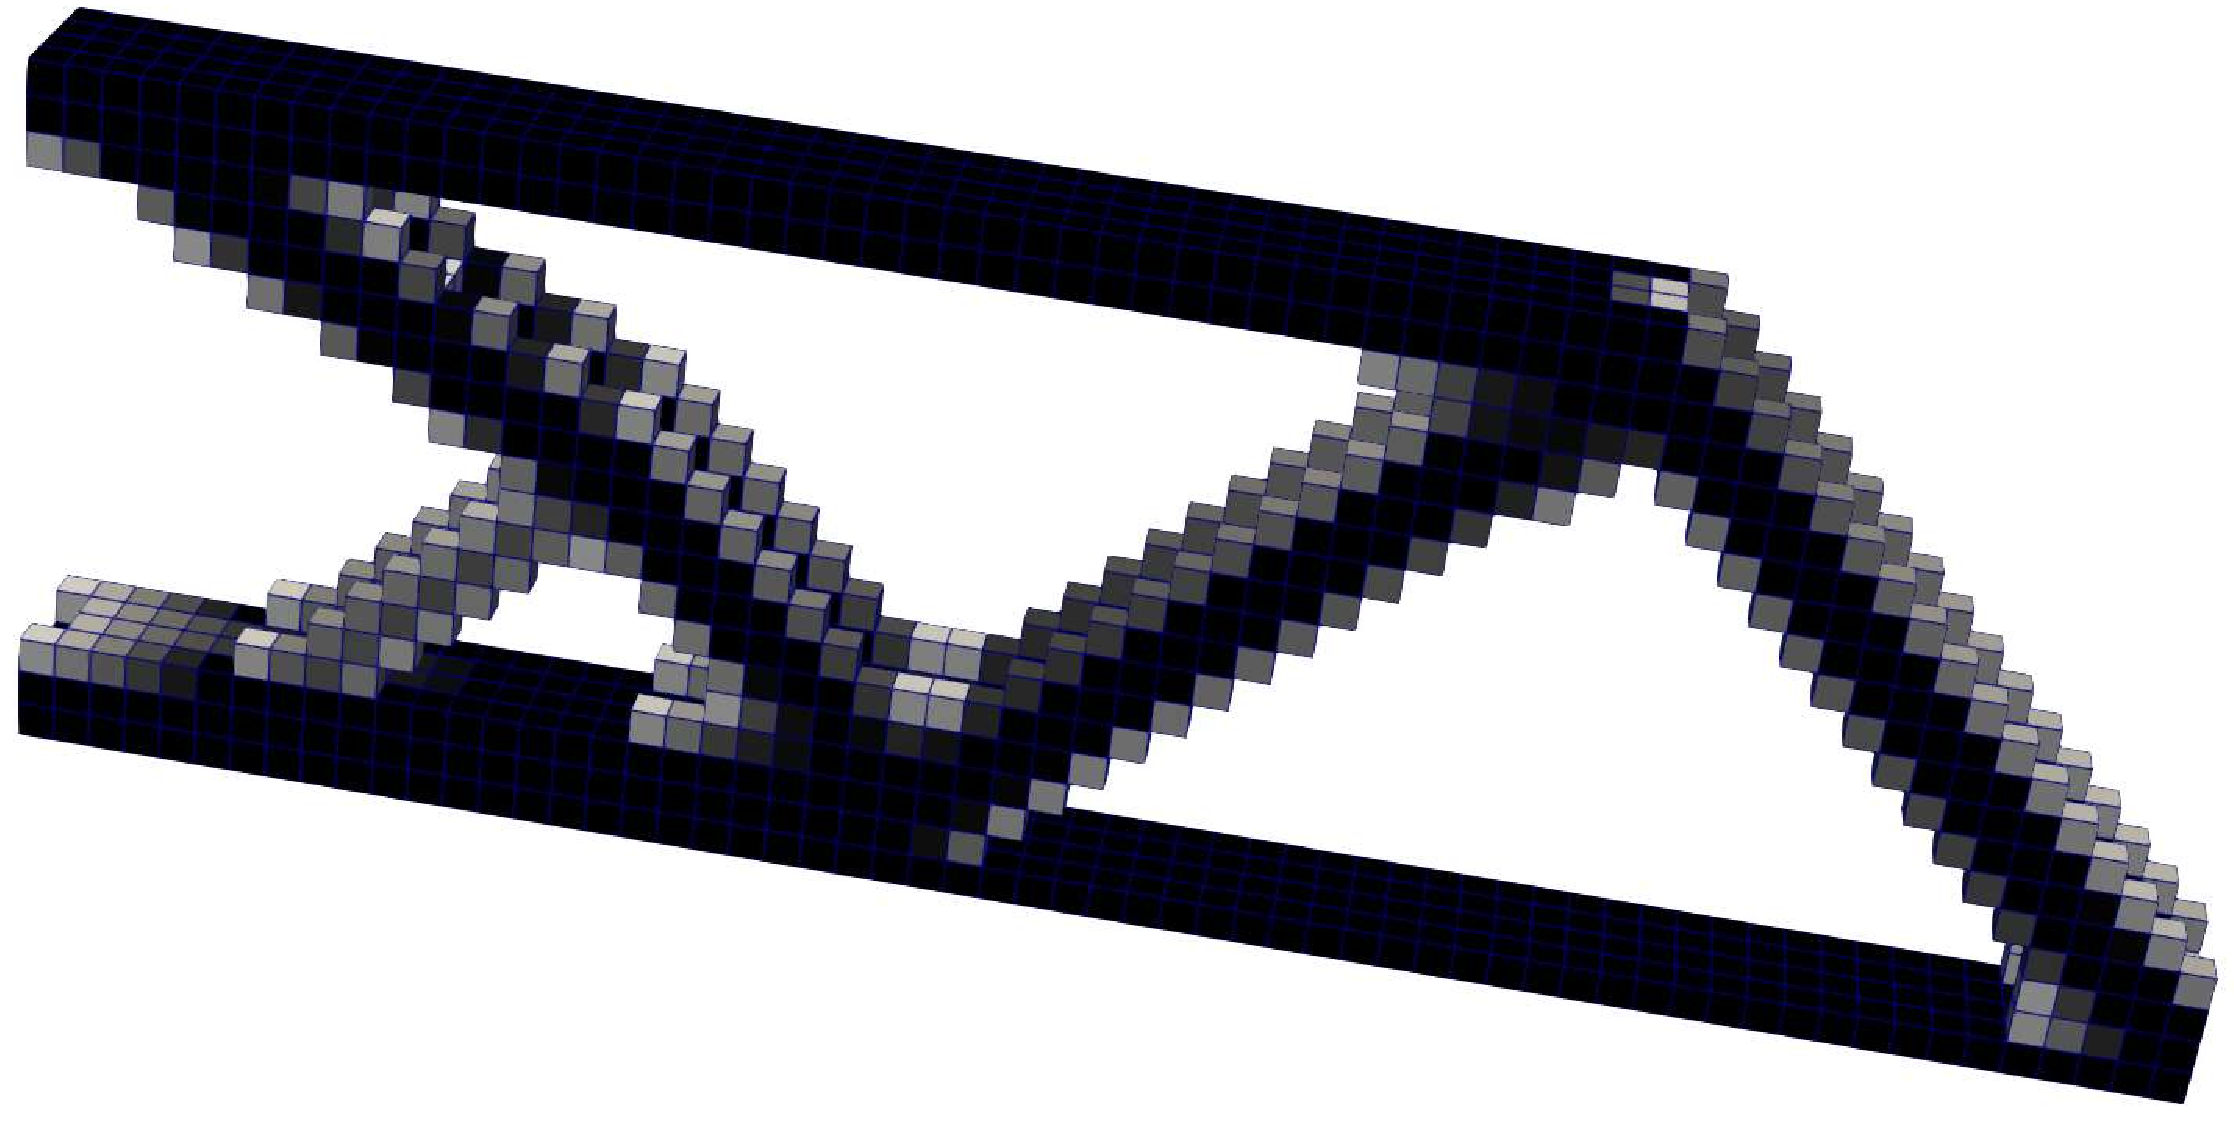
\includegraphics[width=0.95\linewidth,
					height=0.30\paperheight, keepaspectratio]{topo_backend_pytorch}
					
					{\fontsize{8}{11}\selectfont\sffamily (b)\enspace PyTorch}
				\end{column}
				
				\begin{column}{0.32\linewidth}
					\centering
					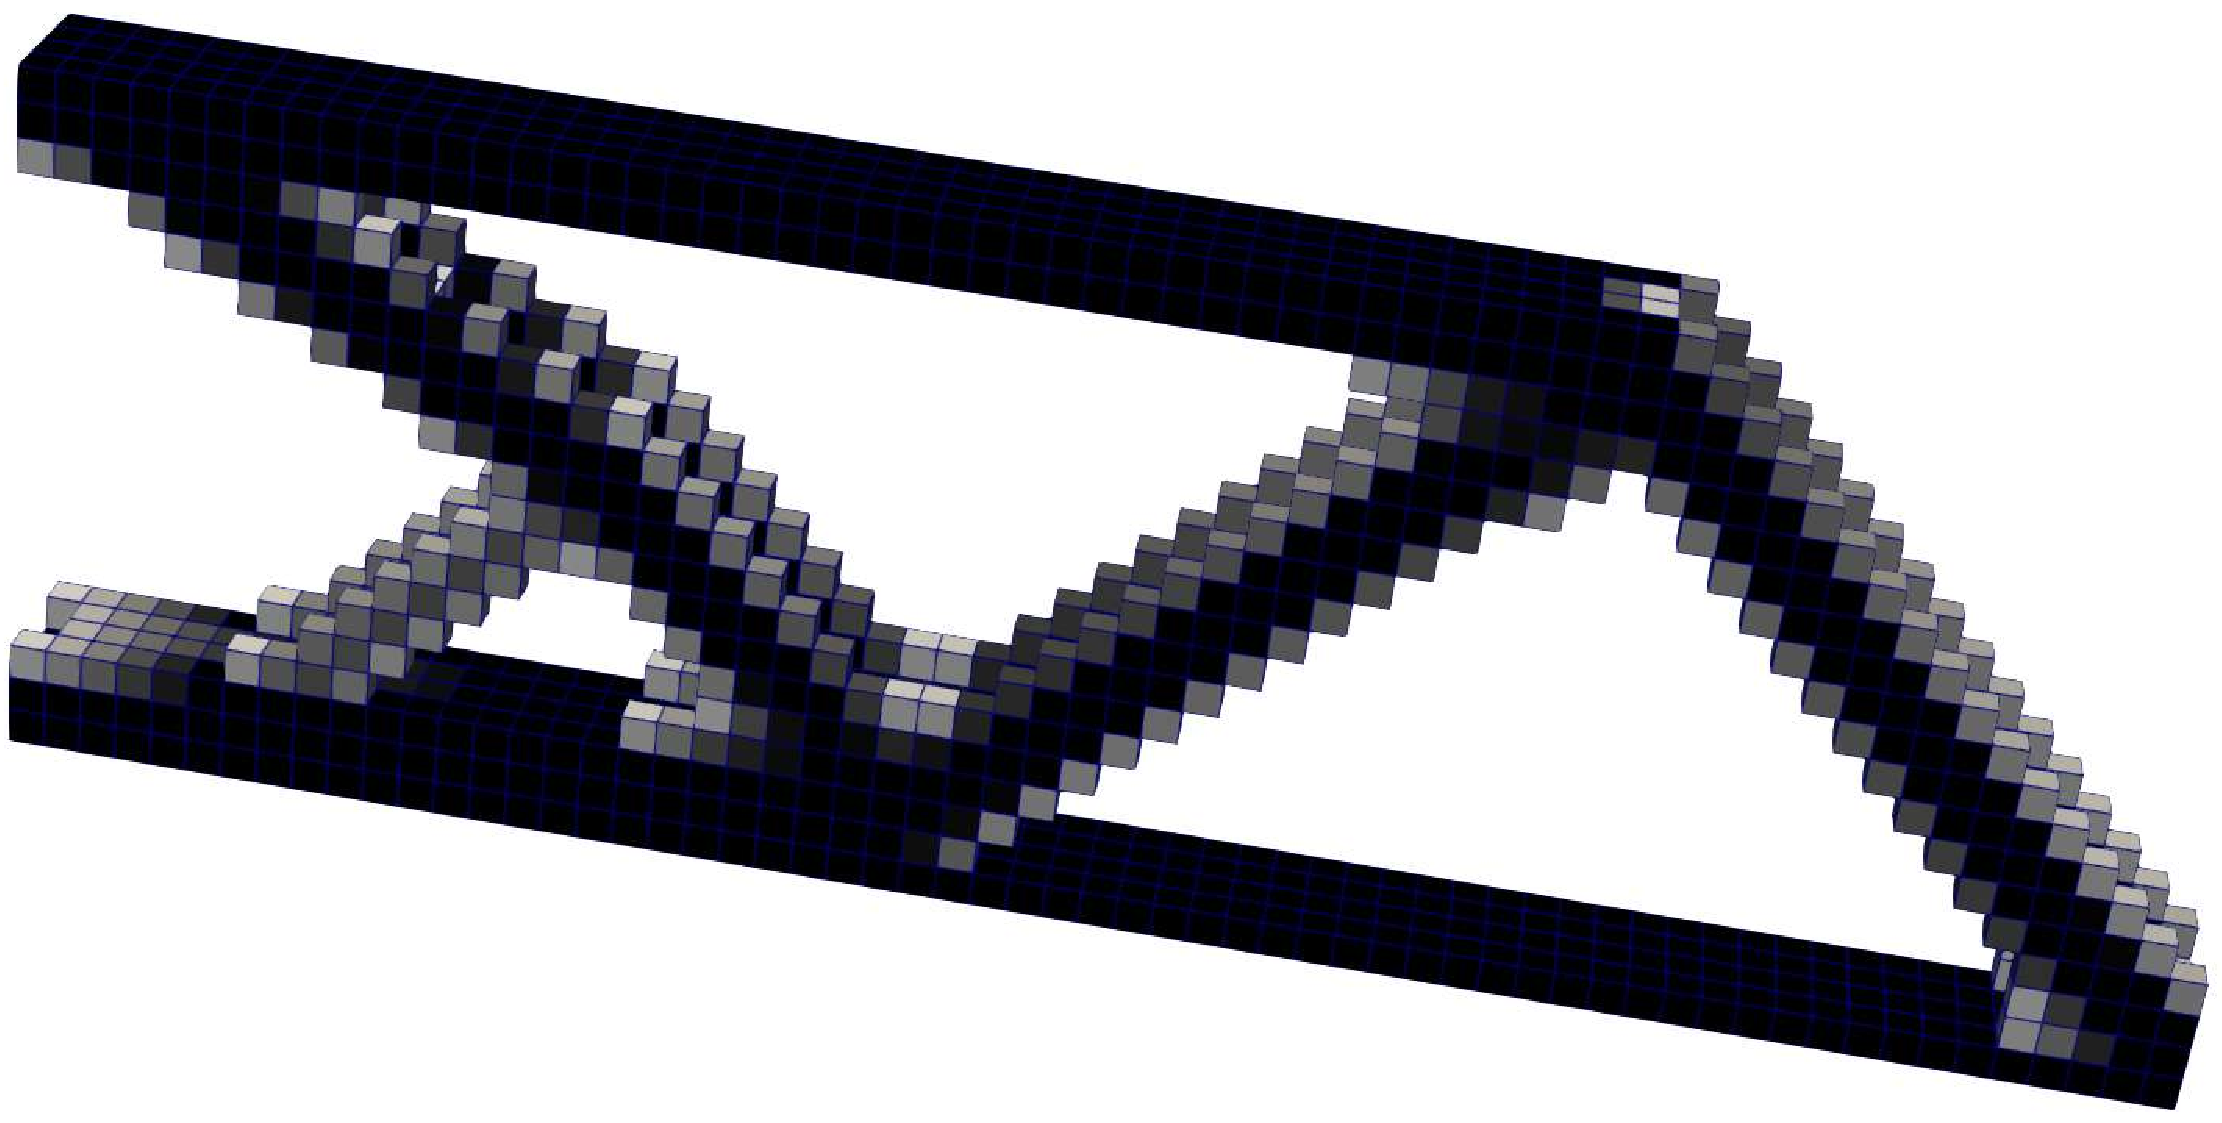
\includegraphics[width=0.95\linewidth,
					height=0.30\paperheight, keepaspectratio]{topo_backend_jax}
					
					{\fontsize{8}{11}\selectfont\sffamily (c)\enspace JAX}
				\end{column}
				
			\end{columns}
			
			\vspace{0.4em}
			
			\begin{tcolorbox}[
				colback=structure.fg, colframe=structure.fg,
				coltext=white, boxrule=0pt, arc=3pt,
				top=4pt, bottom=4pt, left=8pt, right=8pt]
				{\fontsize{7.5}{11}\selectfont\sffamily
					\setlength{\parskip}{0pt}
					\textbf{\circnum{1} 构型一致：}三种后端均获得主承载路径高度一致的三维拓扑构型。
					
					\textbf{\circnum{2} 后端可切换：}同一套高层优化流程可在 \textbf{NumPy}、\textbf{PyTorch} 与 \textbf{JAX} 后端下稳定执行。
				}
			\end{tcolorbox}
		}
		
		% ============================================================
		% Overlay 2：收敛历程一致性
		% ============================================================
		\only<2>{
			
			\begin{center}
				{\fontsize{8.5}{11}\selectfont\sffamily\bfseries
					不同张量后端下三维悬臂梁柔顺度收敛历程}
			\end{center}
			
			\vspace{-0.2em}
			
			\begin{center}
				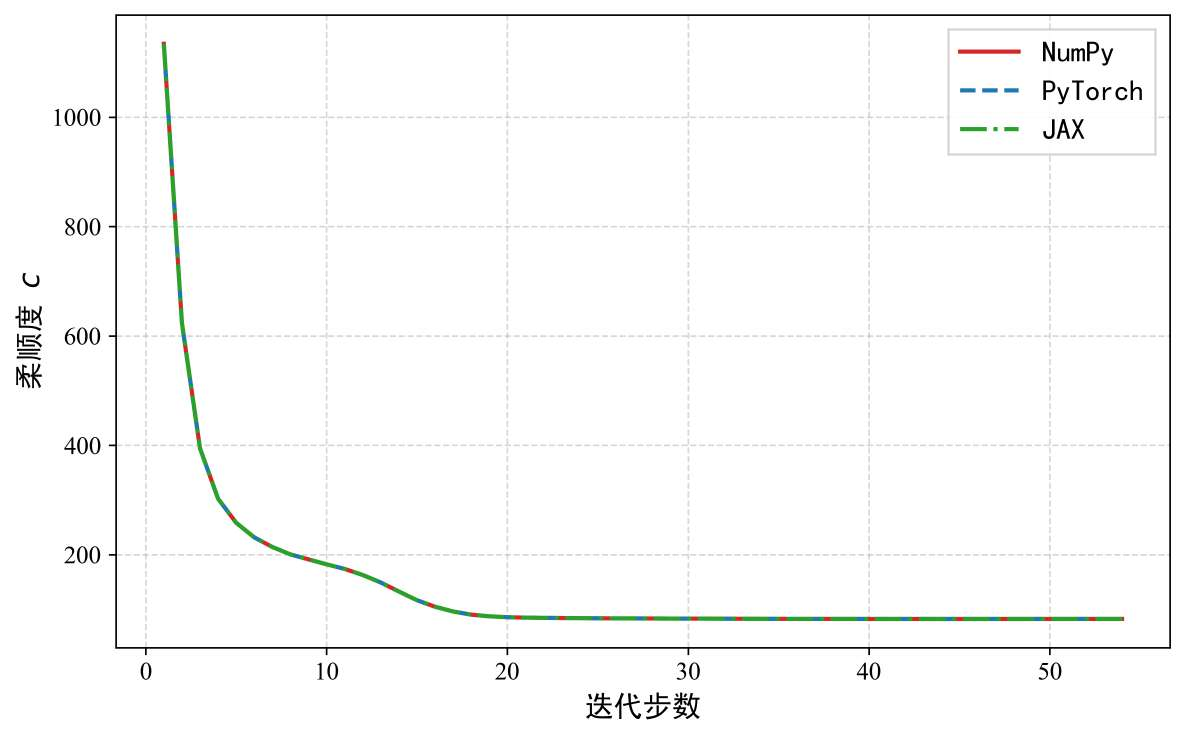
\includegraphics[width=0.78\linewidth,
				height=0.38\paperheight, keepaspectratio]{backend_convergence}
			\end{center}
			
			\vspace{-1.0em}
			
			\begin{tcolorbox}[
				colback=structure.fg, colframe=structure.fg,
				coltext=white, boxrule=0pt, arc=3pt,
				top=4pt, bottom=4pt, left=8pt, right=8pt]
				{\fontsize{7.5}{11}\selectfont\sffamily
					\setlength{\parskip}{0pt}
					\textbf{\circnum{1} 收敛曲线重合：}三条柔顺度下降曲线在全迭代过程中几乎完全重合。
					
					\textbf{\circnum{2} 终止步数一致：}三种后端均在相同终止准则下于第 \textbf{54 步}触发收敛。
				}
			\end{tcolorbox}
		}
		
	\end{frame}
	
	% ============================================================
	%  06-7  CPU/GPU 异构执行与加速性能
	% ============================================================
	
	\begin{frame}
		\frametitle{CPU/GPU 异构执行与加速性能}
		
		% ── 顶部总述条 ──────────────────────────────────────
		\begin{tcolorbox}[
			colback=panelbg, colframe=structure.fg!40,
			arc=3pt, boxrule=0.5pt,
			top=3pt, bottom=3pt, left=8pt, right=8pt]
			{\fontsize{8}{12}\selectfont\sffamily
				依托统一张量抽象接口，SOPTX 可在 CPU/GPU 异构设备间切换，
				并利用 GPU 并行计算能力提升大规模三维拓扑优化效率。}
		\end{tcolorbox}
		
		% ══════════════════════════════════════════════════════════
		%  中部：表格
		% ══════════════════════════════════════════════════════════
		\begin{center}
			{\fontsize{8.5}{11}\selectfont\sffamily\bfseries
				不同设备下三维悬臂梁优化问题的耗时与加速比对比}
			
			\vspace{6pt}
			
			{\fontsize{7.5}{12}\selectfont\sffamily
				\renewcommand{\arraystretch}{1.30}
				\begin{tabular}{@{}l@{\hspace{2em}}c@{\hspace{2em}}c@{\hspace{2em}}c@{\hspace{2em}}c@{\hspace{2em}}c@{}}
					\toprule
					\textbf{设备} & \textbf{总耗时\,/\,s} & \textbf{端到端加速比} & \textbf{首次迭代\,/\,s} & \textbf{后续平均迭代\,/\,s} & \textbf{稳态加速比} \\
					\midrule
					CPU & 2789.927 & --- & 6.443 & 21.087 & --- \\
					GPU & \textbf{636.741} & \textbf{4.38$\times$} & 1.821 & \textbf{4.841} & \textbf{4.36$\times$} \\
					\bottomrule
			\end{tabular}}
		\end{center}
		
		% ══════════════════════════════════════════════════════════
		%  底部：关键结论（一栏三点）
		% ══════════════════════════════════════════════════════════
		\begin{tcolorbox}[
			colback=structure.fg, colframe=structure.fg,
			coltext=white, boxrule=0pt, arc=3pt,
			top=4pt, bottom=4pt, left=8pt, right=8pt]
			{\fontsize{7.5}{11}\selectfont\sffamily
				\setlength{\parskip}{0pt}
				\textbf{\circnum{1} 端到端加速：}GPU 将总耗时由 \textbf{2789.927\,s} 降至 \textbf{636.741\,s}，实现约 \textbf{4.38$\times$} 加速。
				
				\textbf{\circnum{2} 稳态迭代加速：}后续平均迭代耗时由 \textbf{21.087\,s} 降至 \textbf{4.841\,s}，稳态加速比约 \textbf{4.36$\times$}。
				
				\textbf{\circnum{3} 异构计算支撑：}统一张量抽象支持同一优化流程迁移至 GPU 并行执行，为大规模三维问题求解提供支撑。
			}
		\end{tcolorbox}
		
	\end{frame}
	
	
	% ============================================================
	\section{总结与研究展望}
	% ============================================================
	
	% ============================================================
	%  07-1  主要工作与创新贡献
	% ============================================================
	
	\begin{frame}
		\frametitle{主要工作与创新贡献}
		
		% ── 顶部总述条 ──────────────────────────────────────
		\begin{tcolorbox}[
			colback=panelbg, colframe=structure.fg!40,
			arc=3pt, boxrule=0.5pt,
			top=3pt, bottom=3pt, left=8pt, right=8pt]
			{\fontsize{8.0}{11.2}\selectfont\sffamily
				本文围绕连续体结构变密度拓扑优化，形成了
				高阶离散—多分辨率计算—混合建模—软件实现
				的系统研究链条。}
		\end{tcolorbox}
		
		\vspace{-1.0em}
		
		% ══════════════════════════════════════════════════════════
		%  第一行：贡献 01-02
		% ══════════════════════════════════════════════════════════
		\begin{columns}[T, totalwidth=\linewidth]
			
			\begin{column}{0.49\linewidth}
				\begin{tcolorbox}[
					colback=white, colframe=structure.fg!50,
					colbacktitle=structure.fg, coltitle=white,
					fonttitle=\fontsize{7.8}{9.6}\selectfont\bfseries\sffamily,
					title={\circnum{01}\enspace 任意次拉格朗日有限元拓扑优化方法},
					arc=3pt, boxrule=0.5pt,
					toptitle=2pt, bottomtitle=2pt,
					top=4pt, bottom=4pt, left=7pt, right=7pt,
					height=0.28\paperheight]
					{\fontsize{7.1}{9.6}\selectfont\sffamily
						\setbeamertemplate{itemize item}{\raisebox{1pt}{\tiny$\bullet$}}
						\setlength{\leftmargini}{1.0em}
						\begin{itemize}
							\setlength{\itemsep}{2.0pt}
							\setlength{\topsep}{1pt}
							\setlength{\parsep}{0pt}
							\item 建立任意次多单元族拉格朗日有限元离散框架；
							\item 比较单元类型、离散阶次与密度表征方式的影响。
						\end{itemize}
					}
				\end{tcolorbox}
			\end{column}
			
			\begin{column}{0.49\linewidth}
				\begin{tcolorbox}[
					colback=white, colframe=structure.fg!50,
					colbacktitle=structure.fg, coltitle=white,
					fonttitle=\fontsize{7.8}{9.6}\selectfont\bfseries\sffamily,
					title={\circnum{02}\enspace 高阶有限元多分辨率拓扑优化框架},
					arc=3pt, boxrule=0.5pt,
					toptitle=2pt, bottomtitle=2pt,
					top=4pt, bottom=4pt, left=7pt, right=7pt,
					height=0.28\paperheight]
					{\fontsize{7.1}{9.6}\selectfont\sffamily
						\setbeamertemplate{itemize item}{\raisebox{1pt}{\tiny$\bullet$}}
						\setlength{\leftmargini}{1.0em}
						\begin{itemize}
							\setlength{\itemsep}{2.0pt}
							\setlength{\topsep}{1pt}
							\setlength{\parsep}{0pt}
							\item 构建分析网格、密度积分网格与设计网格解耦机制；
							\item 在可控计算规模下兼顾分析精度与拓扑表达分辨率。
						\end{itemize}
					}
				\end{tcolorbox}
			\end{column}
			
		\end{columns}
		
		\vspace{0.35em}
		
		% ══════════════════════════════════════════════════════════
		%  第二行：贡献 03-04
		% ══════════════════════════════════════════════════════════
		\begin{columns}[T, totalwidth=\linewidth]
			
			\begin{column}{0.49\linewidth}
				\begin{tcolorbox}[
					colback=white, colframe=structure.fg!50,
					colbacktitle=structure.fg, coltitle=white,
					fonttitle=\fontsize{7.8}{9.6}\selectfont\bfseries\sffamily,
					title={\circnum{03}\enspace 任意次胡张混合有限元拓扑优化方法},
					arc=3pt, boxrule=0.5pt,
					toptitle=2pt, bottomtitle=2pt,
					top=4pt, bottom=4pt, left=7pt, right=7pt,
					height=0.28\paperheight]
					{\fontsize{7.1}{9.6}\selectfont\sffamily
						\setbeamertemplate{itemize item}{\raisebox{1pt}{\tiny$\bullet$}}
						\setlength{\leftmargini}{1.0em}
						\begin{itemize}
							\setlength{\itemsep}{2.0pt}
							\setlength{\topsep}{1pt}
							\setlength{\parsep}{0pt}
							\item 建立应力--位移混合拓扑优化列式与离散格式；
							\item 提升近不可压缩与局部应力约束问题的计算可靠性。
						\end{itemize}
					}
				\end{tcolorbox}
			\end{column}
			
			\begin{column}{0.49\linewidth}
				\begin{tcolorbox}[
					colback=white, colframe=structure.fg!50,
					colbacktitle=structure.fg, coltitle=white,
					fonttitle=\fontsize{7.8}{9.6}\selectfont\bfseries\sffamily,
					title={\circnum{04}\enspace 多后端拓扑优化软件平台 SOPTX},
					arc=3pt, boxrule=0.5pt,
					toptitle=2pt, bottomtitle=2pt,
					top=4pt, bottom=4pt, left=7pt, right=7pt,
					height=0.28\paperheight]
					{\fontsize{7.1}{9.6}\selectfont\sffamily
						\setbeamertemplate{itemize item}{\raisebox{1pt}{\tiny$\bullet$}}
						\setlength{\leftmargini}{1.0em}
						\begin{itemize}
							\setlength{\itemsep}{2.0pt}
							\setlength{\topsep}{1pt}
							\setlength{\parsep}{0pt}
							\item 依托 FEALPy 构建拓扑优化模块化计算闭环；
							\item 支持自动微分、多后端切换与 CPU/GPU 异构执行。
						\end{itemize}
					}
				\end{tcolorbox}
			\end{column}
			
		\end{columns}
		
	\end{frame}
	
	% ============================================================
	%  07-2  下一步研究安排
	% ============================================================
	
	\begin{frame}
		\frametitle{下一步研究安排}
		
		% ── 顶部总述条 ──────────────────────────────────────
		\begin{tcolorbox}[
			colback=panelbg, colframe=structure.fg!40,
			arc=3pt, boxrule=0.5pt,
			top=3pt, bottom=3pt, left=8pt, right=8pt]
			{\fontsize{8.0}{11.2}\selectfont\sffamily
				在现有高阶有限元、多分辨率计算与 SOPTX 平台基础上，
				后续将面向大规模三维优化、显式几何建模与智能化分析加速，
				构建高性能、可扩展的拓扑优化计算框架。}
		\end{tcolorbox}
		
		\vspace{-1.0em}
		
		% ══════════════════════════════════════════════════════════
		%  第一行：方向 01-02
		% ══════════════════════════════════════════════════════════
		\begin{columns}[T, totalwidth=\linewidth]
			
			% ─── 01 Matrix-free ─────────────────────────────────
			\begin{column}{0.49\linewidth}
				\begin{tcolorbox}[
					colback=white, colframe=structure.fg!50,
					colbacktitle=structure.fg, coltitle=white,
					fonttitle=\fontsize{7.8}{9.6}\selectfont\bfseries\sffamily,
					title={\circnum{01}\enspace GPU 与并行支撑的 Matrix-free 计算},
					arc=3pt, boxrule=0.5pt,
					toptitle=2pt, bottomtitle=2pt,
					top=4pt, bottom=4pt, left=7pt, right=7pt,
					height=0.28\paperheight]
					{\fontsize{7.1}{9.6}\selectfont\sffamily
						\setbeamertemplate{itemize item}{\raisebox{1pt}{\tiny$\bullet$}}
						\setlength{\leftmargini}{1.0em}
						\begin{itemize}
							\setlength{\itemsep}{2.0pt}
							\setlength{\topsep}{1pt}
							\setlength{\parsep}{0pt}
							\item 面向大规模三维拓扑优化，避免反复显式组装全局刚度矩阵；
							\item 结合 GPU 并行算子作用与迭代求解，提升优化闭环计算效率。
						\end{itemize}
					}
				\end{tcolorbox}
			\end{column}
			
			% ─── 02 MMC/MMV ─────────────────────────────────────
			\begin{column}{0.49\linewidth}
				\begin{tcolorbox}[
					colback=white, colframe=structure.fg!50,
					colbacktitle=structure.fg, coltitle=white,
					fonttitle=\fontsize{7.8}{9.6}\selectfont\bfseries\sffamily,
					title={\circnum{02}\enspace 显式拓扑优化方法 MMC/MMV},
					arc=3pt, boxrule=0.5pt,
					toptitle=2pt, bottomtitle=2pt,
					top=4pt, bottom=4pt, left=7pt, right=7pt,
					height=0.28\paperheight]
					{\fontsize{7.1}{9.6}\selectfont\sffamily
						\setbeamertemplate{itemize item}{\raisebox{1pt}{\tiny$\bullet$}}
						\setlength{\leftmargini}{1.0em}
						\begin{itemize}
							\setlength{\itemsep}{2.0pt}
							\setlength{\topsep}{1pt}
							\setlength{\parsep}{0pt}
							\item 引入移动可变形组件/孔洞方法，直接描述结构边界与几何构型；
							\item 探索显式几何表达与高阶有限元、多分辨率框架的结合。
						\end{itemize}
					}
				\end{tcolorbox}
			\end{column}
			
		\end{columns}
		
		\vspace{0.35em}
		
		% ══════════════════════════════════════════════════════════
		%  第二行：方向 03-04
		% ══════════════════════════════════════════════════════════
		\begin{columns}[T, totalwidth=\linewidth]
			
			% ─── 03 PIML ────────────────────────────────────────
			\begin{column}{0.49\linewidth}
				\begin{tcolorbox}[
					colback=white, colframe=structure.fg!50,
					colbacktitle=structure.fg, coltitle=white,
					fonttitle=\fontsize{7.8}{9.6}\selectfont\bfseries\sffamily,
					title={\circnum{03}\enspace 问题无关机器学习 PIML},
					arc=3pt, boxrule=0.5pt,
					toptitle=2pt, bottomtitle=2pt,
					top=4pt, bottom=4pt, left=7pt, right=7pt,
					height=0.28\paperheight]
					{\fontsize{7.1}{9.6}\selectfont\sffamily
						\setbeamertemplate{itemize item}{\raisebox{1pt}{\tiny$\bullet$}}
						\setlength{\leftmargini}{1.0em}
						\begin{itemize}
							\setlength{\itemsep}{2.0pt}
							\setlength{\topsep}{1pt}
							\setlength{\parsep}{0pt}
							\item 构建与边界条件、载荷和设计域弱相关的局部算子学习模型；
							\item 加速高频重复的局部分析过程，提升拓扑优化计算效率。
						\end{itemize}
					}
				\end{tcolorbox}
			\end{column}
			
			% ─── 04 融合框架 ─────────────────────────────────
			\begin{column}{0.49\linewidth}
				\begin{tcolorbox}[
					colback=white, colframe=structure.fg!50,
					colbacktitle=structure.fg, coltitle=white,
					fonttitle=\fontsize{7.8}{9.6}\selectfont\bfseries\sffamily,
					title={\circnum{04}\enspace 高性能智能拓扑优化融合框架},
					arc=3pt, boxrule=0.5pt,
					toptitle=2pt, bottomtitle=2pt,
					top=4pt, bottom=4pt, left=7pt, right=7pt,
					height=0.28\paperheight]
					{\fontsize{7.1}{9.6}\selectfont\sffamily
						\setbeamertemplate{itemize item}{\raisebox{1pt}{\tiny$\bullet$}}
						\setlength{\leftmargini}{1.0em}
						\begin{itemize}
							\setlength{\itemsep}{2.0pt}
							\setlength{\topsep}{1pt}
							\setlength{\parsep}{0pt}
							\item 将 Matrix-free、MMC/MMV 与 PIML 统一到 SOPTX 框架中；
							\item 面向复杂三维结构设计，形成可扩展的智能优化工具链。
						\end{itemize}
					}
				\end{tcolorbox}
			\end{column}
			
		\end{columns}
		
	\end{frame}
	
	
	% ============================================================
	%  结束页：致谢
	% ============================================================
	
	\begin{frame}[plain]
		
		\vspace*{0.75cm}
		
		\begin{center}
			% ── 标题 ─────────────────────────────────────
			{\fontsize{28}{34}\selectfont
				\bfseries\sffamily\color{structure.fg}
				致\hspace{1.2em}谢}
			
			\vspace{1.55cm}
			
			% ── 主体感谢语 ───────────────────────────────
			\begin{minipage}{0.82\linewidth}
				\centering
				
				{\fontsize{16}{25}\selectfont\sffamily
					衷心感谢各位答辩委员会专家、教授}
				
				\vspace{0.45cm}
				
				{\fontsize{16}{25}\selectfont\sffamily
					对本论文的审阅、指导与宝贵建议！}
				
				\vspace{1.00cm}
				
				{\fontsize{12}{19}\selectfont\sffamily\color{black!55}
					感谢导师、同门以及团队在论文工作中的帮助与支持。}
				
				\vspace{0.95cm}
				
				{\fontsize{18}{25}\selectfont
					\bfseries\sffamily\color{structure.fg}
					敬请各位专家批评指正！}
				
			\end{minipage}
			
		\end{center}
		
	\end{frame}
	
	
\end{document}